% Options for packages loaded elsewhere
\PassOptionsToPackage{unicode}{hyperref}
\PassOptionsToPackage{hyphens}{url}
\PassOptionsToPackage{dvipsnames,svgnames,x11names}{xcolor}
%
\documentclass[
  12pt,
  letterpaper,
  twoside]{book}
\usepackage{amsmath,amssymb}
\usepackage[]{times}
\usepackage{setspace}
\usepackage{iftex}
\ifPDFTeX
  \usepackage[T1]{fontenc}
  \usepackage[utf8]{inputenc}
  \usepackage{textcomp} % provide euro and other symbols
\else % if luatex or xetex
  \usepackage{unicode-math}
  \defaultfontfeatures{Scale=MatchLowercase}
  \defaultfontfeatures[\rmfamily]{Ligatures=TeX,Scale=1}
\fi
% Use upquote if available, for straight quotes in verbatim environments
\IfFileExists{upquote.sty}{\usepackage{upquote}}{}
\IfFileExists{microtype.sty}{% use microtype if available
  \usepackage[]{microtype}
  \UseMicrotypeSet[protrusion]{basicmath} % disable protrusion for tt fonts
}{}
\makeatletter
\@ifundefined{KOMAClassName}{% if non-KOMA class
  \IfFileExists{parskip.sty}{%
    \usepackage{parskip}
  }{% else
    \setlength{\parindent}{0pt}
    \setlength{\parskip}{6pt plus 2pt minus 1pt}}
}{% if KOMA class
  \KOMAoptions{parskip=half}}
\makeatother
\usepackage{xcolor}
\usepackage[tmargin=2.5cm,bmargin=2.5cm,lmargin=2.5cm,rmargin=2.5cm,headheight=2.5cm,bottom=2.5cm]{geometry}
\usepackage{color}
\usepackage{fancyvrb}
\newcommand{\VerbBar}{|}
\newcommand{\VERB}{\Verb[commandchars=\\\{\}]}
\DefineVerbatimEnvironment{Highlighting}{Verbatim}{commandchars=\\\{\}}
% Add ',fontsize=\small' for more characters per line
\usepackage{framed}
\definecolor{shadecolor}{RGB}{248,248,248}
\newenvironment{Shaded}{\begin{snugshade}}{\end{snugshade}}
\newcommand{\AlertTok}[1]{\textcolor[rgb]{0.94,0.16,0.16}{#1}}
\newcommand{\AnnotationTok}[1]{\textcolor[rgb]{0.00,0.00,0.00}{\textit{#1}}}
\newcommand{\AttributeTok}[1]{\textcolor[rgb]{0.48,0.12,0.64}{#1}}
\newcommand{\BaseNTok}[1]{\textcolor[rgb]{0.28,0.53,0.93}{#1}}
\newcommand{\BuiltInTok}[1]{#1}
\newcommand{\CharTok}[1]{\textcolor[rgb]{0.87,0.29,0.22}{#1}}
\newcommand{\CommentTok}[1]{\textcolor[rgb]{0.24,0.58,0.00}{\textit{#1}}}
\newcommand{\CommentVarTok}[1]{\textcolor[rgb]{0.24,0.58,0.00}{\textit{#1}}}
\newcommand{\ConstantTok}[1]{\textcolor[rgb]{0.00,0.00,0.00}{#1}}
\newcommand{\ControlFlowTok}[1]{\textcolor[rgb]{0.00,0.00,0.00}{\textbf{#1}}}
\newcommand{\DataTypeTok}[1]{\textcolor[rgb]{0.00,0.00,0.00}{#1}}
\newcommand{\DecValTok}[1]{\textcolor[rgb]{0.28,0.53,0.93}{#1}}
\newcommand{\DocumentationTok}[1]{\textcolor[rgb]{0.56,0.35,0.01}{\textit{#1}}}
\newcommand{\ErrorTok}[1]{\textcolor[rgb]{0.64,0.00,0.00}{#1}}
\newcommand{\ExtensionTok}[1]{#1}
\newcommand{\FloatTok}[1]{\textcolor[rgb]{0.28,0.53,0.93}{#1}}
\newcommand{\FunctionTok}[1]{\textcolor[rgb]{0.48,0.12,0.64}{#1}}
\newcommand{\ImportTok}[1]{#1}
\newcommand{\InformationTok}[1]{\textcolor[rgb]{0.00,0.00,0.00}{\textit{#1}}}
\newcommand{\KeywordTok}[1]{\textcolor[rgb]{0.48,0.12,0.64}{#1}}
\newcommand{\NormalTok}[1]{#1}
\newcommand{\OperatorTok}[1]{\textcolor[rgb]{0.00,0.00,0.00}{#1}}
\newcommand{\OtherTok}[1]{\textcolor[rgb]{0.04,0.84,0.78}{#1}}
\newcommand{\PreprocessorTok}[1]{\textcolor[rgb]{0.00,0.00,0.00}{\textit{#1}}}
\newcommand{\RegionMarkerTok}[1]{#1}
\newcommand{\SpecialCharTok}[1]{\textcolor[rgb]{0.87,0.29,0.22}{#1}}
\newcommand{\SpecialStringTok}[1]{\textcolor[rgb]{0.31,0.60,0.02}{#1}}
\newcommand{\StringTok}[1]{\textcolor[rgb]{0.87,0.29,0.22}{#1}}
\newcommand{\VariableTok}[1]{\textcolor[rgb]{0.00,0.00,0.00}{#1}}
\newcommand{\VerbatimStringTok}[1]{\textcolor[rgb]{0.48,0.12,0.64}{#1}}
\newcommand{\WarningTok}[1]{\textcolor[rgb]{0.00,0.00,0.00}{\textit{#1}}}
\usepackage{longtable,booktabs,array}
\usepackage{calc} % for calculating minipage widths
% Correct order of tables after \paragraph or \subparagraph
\usepackage{etoolbox}
\makeatletter
\patchcmd\longtable{\par}{\if@noskipsec\mbox{}\fi\par}{}{}
\makeatother
% Allow footnotes in longtable head/foot
\IfFileExists{footnotehyper.sty}{\usepackage{footnotehyper}}{\usepackage{footnote}}
\makesavenoteenv{longtable}
\usepackage{graphicx}
\makeatletter
\def\maxwidth{\ifdim\Gin@nat@width>\linewidth\linewidth\else\Gin@nat@width\fi}
\def\maxheight{\ifdim\Gin@nat@height>\textheight\textheight\else\Gin@nat@height\fi}
\makeatother
% Scale images if necessary, so that they will not overflow the page
% margins by default, and it is still possible to overwrite the defaults
% using explicit options in \includegraphics[width, height, ...]{}
\setkeys{Gin}{width=\maxwidth,height=\maxheight,keepaspectratio}
% Set default figure placement to htbp
\makeatletter
\def\fps@figure{htbp}
\makeatother
\setlength{\emergencystretch}{3em} % prevent overfull lines
\providecommand{\tightlist}{%
  \setlength{\itemsep}{0pt}\setlength{\parskip}{0pt}}
\setcounter{secnumdepth}{5}
\pagestyle{empty}
\usepackage{graphicx}
\usepackage{array}
%%%
%\usepackage{makeidx}
% Para numeración de páginas
\usepackage{fancyhdr}
% Para cuadros de tips
\usepackage{tcolorbox}
\usepackage{awesomebox}
%\usepackage{titling}
% Para fonts, encoding e idioma
\usepackage{lmodern}
\usepackage[utf8]{inputenc}
\usepackage[T1]{fontenc}
\usepackage[spanish, mexico]{babel}
% Agregar guión a palabras que no quepan
\usepackage[none]{hyphenat}
% Control de títulos en el texto
\usepackage[newparttoc]{titlesec}
% Control de títulos en el table of contents
% Mejor usar este en lugar de tocloft
%\usepackage{titletoc}
% Para el control de viudas y huerfanos
\usepackage[defaultlines=4,all]{nowidow}
%\usepackage{flafter}
% Para poner figuras en floats
\usepackage{float}
% Para manejo de índice
\usepackage[titles]{tocloft}
\usepackage{makeidx}
\usepackage{pdfpages}
\usepackage{multicol}
\usepackage{tikz}
%\usepackage[abs]{overpic}
%\usepackage{pict2e}
%\usepackage{hanging}


\addtocontents{toc}{\protect\thispagestyle{fancy}}
\renewcommand{\cftdot}{}

%\makeindex
%\floatplacement{figure}{btp}

% Definir colores
\definecolor{lightblue}{RGB}{222,243,247}
\definecolor{darkblue}{RGB}{29,77,86}
\definecolor{abvrulecolor}{RGB}{22,92,105}
\definecolor{darkpurple}{RGB}{123,31,162}
\definecolor{red}{RGB}{221,75,57}
\definecolor{blue}{RGB}{71,135,237}

% Captions de figuras
% Cambiar el color para los títulos de figuras
\usepackage[labelfont={color=darkblue,bf},singlelinecheck=off,center]{caption}

% Re definir títulos y formato con titlesec
\renewcommand{\chaptermark}[1]{\markboth{#1}{}}
\renewcommand{\sectionmark}[1]{\markright{#1}{}}
\titlelabel{\thetitle\quad}
\titleformat{\chapter}{\normalfont\LARGE\bfseries\color{darkblue}}{\thechapter}{1em}{}
\titleformat*{\section}{\normalfont\Large\bfseries\color{darkblue}}
\titleformat*{\subsection}{\normalfont\large\bfseries\color{darkblue}}
\titleformat*{\subsubsection}{\normalfont\normalsize\bfseries\color{darkblue}}

% title spacings
\titlespacing*{\chapter}{0pt}{2.5ex}{2.5ex}
\titlespacing{\title}{0pt}{\parskip}{-\parskip}

% Pa definir formato de los table of contents con titletoc
% Capítulo, espacio de izquierda entre número y capítulo
%\titlecontents{chapter}[1.4em]{\large\bfseries}
% Numbered entry format
%{\contentslabel[{\thecontentslabel}]{1.5em}}{}
% Filter page format and below code in brackets
%{\titlerule*[1pc]{}\contentspage}[\addvspace{6pt}]
% Aumentar espacio entre número y letras de capítulos

% Secciones
% Name of section to edit, left spacing, vertical spacing
%\titlecontents{section}[3.9 em]{\vspace{-0.3cm}}
%{}{}
%{\contentslabel[{\thecontentslabel}]{2.3em}}{}
%{\titlerule*[0.7pc]{}\contentspage}[\addvspace{4pt}]

% Definir cajas de color
\newtcolorbox{bluebox2}{
  colback=lightblue,
  colframe=darkblue,
  coltext=black,
  boxsep=0pt,
  arc=0pt
}

\newtcolorbox{blackbox}{
  colback=white,
  colframe=black,
  coltext=black,
  boxsep=0pt,
  arc=0pt
}

% Formato de página
\renewcommand\headrulewidth{0pt}
%
\pagestyle{empty}
  \fancyhf{}
\fancypagestyle{plain}{}
\fancypagestyle{fancy}{}
%\fancypagestyle{toc}{}
%\fancypagestyle{main}{}
%\fancypagestyle{contents}{}

% Para ayudar a que el float sea menos agresivo
\renewcommand{\topfraction}{.8}
\renewcommand{\bottomfraction}{.8}
\renewcommand{\textfraction}{.05}
\renewcommand{\floatpagefraction}{.75}

% Para modificar los colores del table of contents to tocloft
% Title TOC color
\renewcommand{\cfttoctitlefont}{\normalfont\LARGE\bfseries\color{darkblue}}
\renewcommand{\cftpartfont}{\bfseries\color{darkblue}} % tocloft
%\renewcommand{\cftchapfont}{\bfseries\color{darkblue}} % tocloft
%\renewcommand{\cftchappagefont}{\color{darkblue}} % tocloft
%\renewcommand{\cftchappresnum}{\bfseries\color{darkblue}} % tocloft
%\renewcommand{\cftchapaftersnum}{\bfseries\color{darkblue}}
%\renewcommand{\cftchapfont}{\bfseries\Color{darkblue}}% Chapter colour
%\renewcommand{\cftsecfont}{\Color{black}}% Section colour
%\renewcommand{\cftsubsecfont}{\Color{black}}% Subsection colour

% Spacing using tocloft
\advance\cftsecnumwidth 0.5em\relax
\advance\cftsubsecindent 0.5em\relax
\advance\cftsubsecnumwidth 0.5em\relax

\newcommand\boldpurple[1]{\textcolor{darkpurple}{\textbf{#1}}}

\newenvironment{Figure}
  {\par\medskip\noindent\minipage{\linewidth}}
  {\endminipage\par\medskip}
% Tratar de cambiar lista de tablas a ejercicios
%\renewcommand{\listtablename}{Lista de Ejercicios}

%\renewcommand{\familydefault}{\rmdefault}
%\renewcommand{\ttdefault}{\ttdefault}

%\renewcommand\headrulewidth{1pt}
%\pagestyle{fancy} 
%  \fancyfoot{}
%  \fancyfoot[LE,RO]{\thepage}
%  \fancyhead{}
%  \fancyhead[LE,RO]{\leftmark}
%  \fancyhead[LO,RE]{\rightmark}
%\fancypagestyle{plain}{}
\makeindex
%\indexsetup
%\renewcommand{\indexsetup}{firstpagestyle=fancy}

% Try to fix the problem of text being moved to occupy whole page
\raggedbottom

% Para agregar páginas al principio
\let\oldmaketitle\maketitle
\AtBeginDocument{\let\maketitle\relax}
\ifLuaTeX
  \usepackage{selnolig}  % disable illegal ligatures
\fi
\IfFileExists{bookmark.sty}{\usepackage{bookmark}}{\usepackage{hyperref}}
\IfFileExists{xurl.sty}{\usepackage{xurl}}{} % add URL line breaks if available
\urlstyle{same} % disable monospaced font for URLs
\hypersetup{
  pdftitle={Cómo usar Google Earth Engine y no fallar en el intento},
  pdfauthor={Jonathan Vidal Solórzano Villegas y Gabriel Alejandro Perilla Suárez},
  colorlinks=true,
  linkcolor={darkblue},
  filecolor={Maroon},
  citecolor={Blue},
  urlcolor={darkblue},
  pdfcreator={LaTeX via pandoc}}

\title{Cómo usar Google Earth Engine y no fallar en el intento}
\author{Jonathan Vidal Solórzano Villegas y Gabriel Alejandro Perilla Suárez}
\date{}

\begin{document}
\maketitle

\thispagestyle{empty}
\begin{center}
%{\Huge A BOOK}
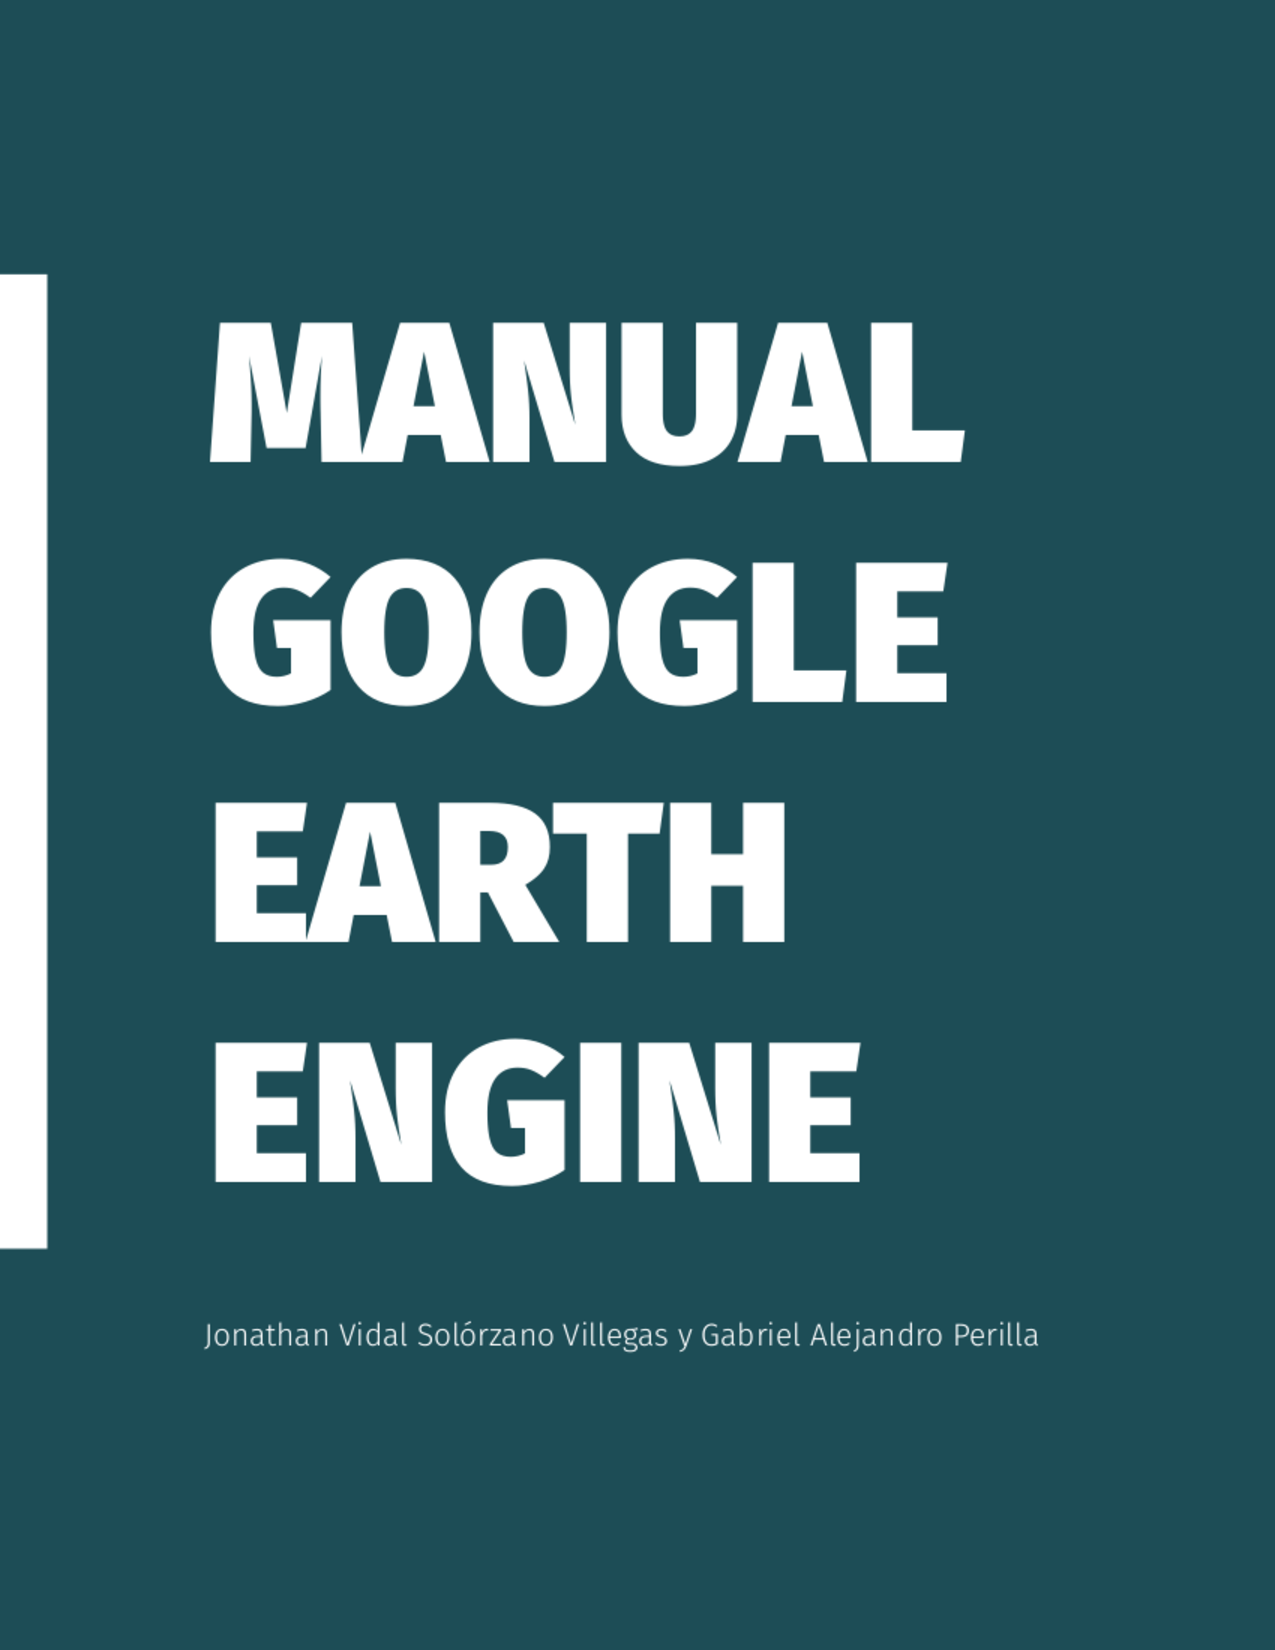
\includepdf{Img/Portada.pdf}
%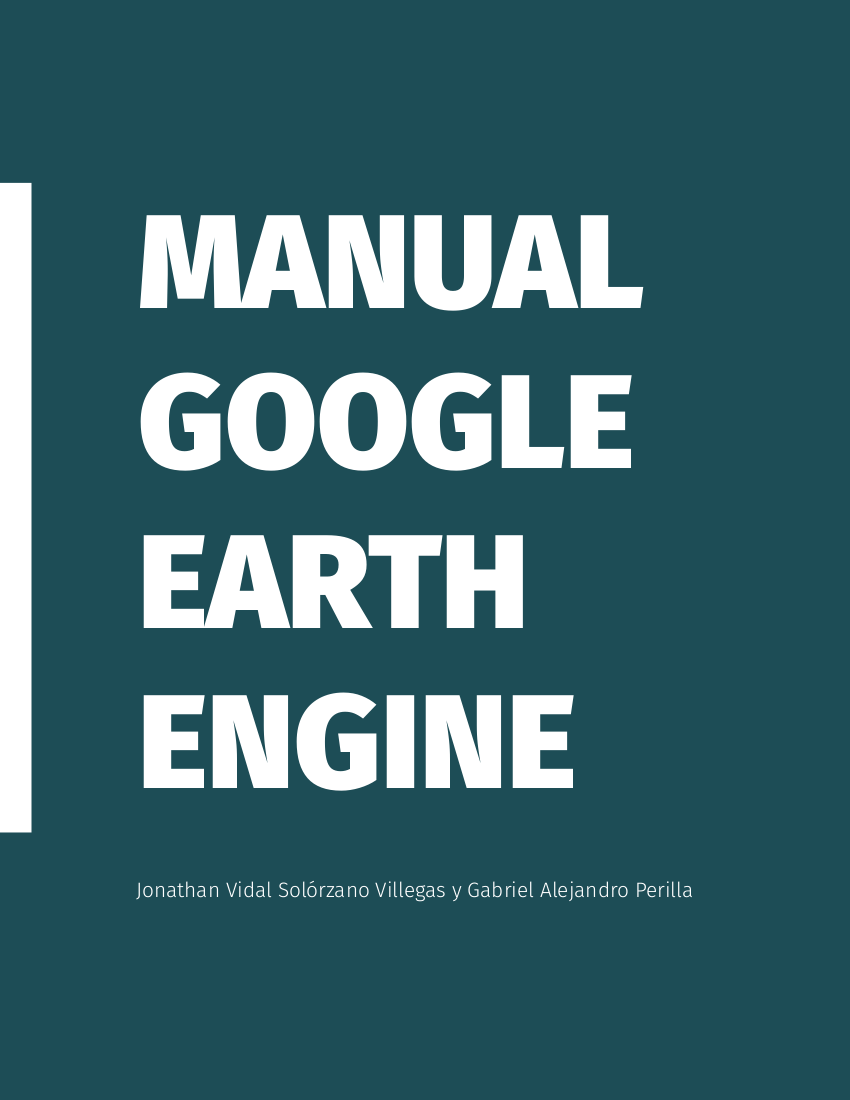
\includegraphics{Img/Portada.png}
%{\huge by Jonathan Vidal Solórzano Villegas y Alejandro Perilla Suárez}
\end{center}

% Título
\newpage
\topskip0pt
\vspace*{\fill}
\begin{center}
\LARGE{Cómo usar Google Earth Engine y no fallar en el intento}
\end{center}
\vspace*{\fill}

% Instituciones
\newpage

\topskip0pt
\vspace*{\fill}
\begin{center}
\large{Centro de Investigaciones en Geografía Ambiental}
\linebreak
\large{Universidad Nacional Autónoma de México}
\linebreak
\large{Instituto de Investigación de Recursos Biológicos Alexander von Humboldt}
\end{center}
\vspace*{\fill}

% Logos
\newpage

\topskip0pt
\vspace*{\fill}
\begin{center}
\LARGE{Cómo usar Google Earth Engine y no fallar en el intento}
\linebreak
\linebreak
\large{Jonathan Vidal Solórzano Villegas y Gabriel Alejandro Perilla Suárez}
\end{center}
\vspace{15mm}
\setlength{\columnsep}{40pt}
\begin{multicols}{2}
%\noindent
    \begin{Figure}
    \centering
    
\includegraphics[width=0.7\linewidth]{Img/unam}
    %\captionof{figure}{my caption of the figure}
    \end{Figure}
    \centering Universidad Nacional Autónoma de México
    %\columnbreak
    \begin{Figure}
    \centering
    
\includegraphics[width=0.7\linewidth]{Img/humb}
    %\captionof{figure}{my caption of the figure}
    \end{Figure}
    \centering Instituto de Investigación de Recursos Biológicos Alexander von Humboldt 
\end{multicols}
\vspace*{\fill}

% Página legal
\newpage

\topskip0pt
\vspace*{\fill}
\begin{center}
    \begin{blackbox}
        {\footnotesize \textbf{Catalogación en la publicación UNAM. Dirección General de Bibliotecas y Servicios Digitales de Información}

            \textbf{Nombres:} Solórzano Villegas, Jonathan Vidal, autor. | Perilla Suárez, Gabriel Alejandro, autor.  

            \textbf{Título:} Cómo usar Google Earth Engine y no fallar en el intento / Jonathan Vidal Solórzano Villegas y Gabriel Alejandro Perilla Suárez.

            \textbf{Descripción:} Primera edición. | Morelia, Michoacán de Ocampo : Universidad Nacional Autónoma de México, Centro de Investigaciones en Geografía Ambiental ; Bogotá, Colombia : Instituto de Investigación de Recursos Biológicos Alexander von Humboldt, 2022.  
            
            \textbf{Identificadores:} LIBRUNAM 2167765 (libro electrónico) | ISBN 978-607-30-6696-9 (libro electrónico) (UNAM) | ISBN 978-958-5183-55-1 (libro electrónico) (Colombia).    
            
            \textbf{Temas:} Computación en nube. | Sistemas de información geográfica. | Almacenamiento de datos. | Google Earth Engine (Programa para computadora). 
            
            \textbf{Clasificación:} LCC QA76.585 (libro electrónico) | DDC 004.6782—dc23}
        
    \end{blackbox}

    \begin{blackbox}
        {\footnotesize \textbf{Catalogación en la publicación Instituo Alexander Von Humboldt. Biblioteca Francisco Javier Matís}

            Cómo usar Google Earth Engine y no fallar en el intento / Jonathan Vidal Solórzano Villegas, Gabriel Alejandro Perilla Suárez – 1 edición. - Bogotá, D.C. Instituto de Investigación de Recursos Biológicos Alexander von Humboldt, 2022.  
            
                177 páginas.
                Incluye referencias bibliográficas, imágenes, tablas, gráficas
                ISBN digital: 978-958-5183-55-1
            
            1. Programa informático 2. Estructuras de datos 3. Datos geoespaciales 4. Análisis de datos medioambientales 5. Tecnología geoespacial 6. Guía introductoria I. Solórzano Villegas, Jonathan Vidal II. Perilla Suárez, Gabriel Alejandro III. Instituto de Investigación de Recursos Biológicos Alexander von Humboldt. 
            
            Número de contribución: 624
            Registro en el catálogo Humboldt: 15062    
            
            CEP – Biblioteca Francisco Javier Matís - Instituto Alexander von Humboldt}
        
    \end{blackbox}
\end{center}
\vspace*{\fill}

\newpage

\setlength{\columnsep}{25pt}
\begin{multicols*}{2}
    \raggedcolumns
    {\scriptsize Este libro ha sido arbitrado por pares académicos y fue posible gracias al Proyecto PE117519-Programa de Apoyo a Proyectos para la Innovación y Mejoramiento a la Enseñanza (PAPIME), DGAPA, UNAM. 
    \linebreak Este trabajo tiene algunos derechos reservados según lo especifica la licencia internacional {\it Creative Commons Attribution Non Commercial Share Alike 4.0 (CC-BY-NC-SA)}, la cual puede consultar en \href{https://creativecommons.org/licenses/by-nc-sa/4.0/legalcode.es}{https://creativecommons.org/licenses/by-nc} \href{https://creativecommons.org/licenses/by-nc -sa/4.0/legalcode.es}{-sa/4.0/legalcode.es}
    \linebreak
    \linebreak
    %\vfill
    %\medskip
    \begingroup
        
\includegraphics[height=28pt]{Img/license}
    \endgroup
    \newline Diseño editorial: Jonathan Vidal Solórzano Villegas y Laura Perilla Suárez (\href{https://behance.net/lauuuuperilla}{behance.net/lauuuuperilla}).
    \newline Imagen en portada y la contraportada: 20181227T151659\_2 0181227T151707\_19PBN (Sentinel-2) modificada de datos Copernicus Sentinel-2 registrados en 2018/12/27. 
    \newline Imágenes: todas las imágenes fueron creadas por los autores, los screenshots pueden contener pequeñas anotaciones con fines aclaratorios para los usuarios, estas imágenes cumplieron con las pautas y uso de marca de Google, de modo que aplican los términos y condiciones de marca registradas. 
    \newline Todos los nombres de marcas y productos mencionados en esta obra están sujetos a la protección de marcas comerciales, marcas o patentes y las marcas comerciales o marcas comerciales registradas por sus respectivos titulares. 
    El uso de nombres de marca, nombres de productos, nombres comunes, nombres comerciales, descripciones, etc. incluso sin una marca particular en este trabajo no puede de ninguna manera interpretarse en el sentido de que dichos nombres pueden considerarse sin restricciones con respecto a la legislación sobre marcas comerciales y protección de marcas y, por lo tanto, podrían ser utilizados por cualquiera.
    \linebreak
    \newline Revisión académica: Andrea Pamela Flores, Victoria Nazarena Guzmán, Sandra Lucía Hernández Zetina, Xanat Antonio Némiga. \hspace*{\fill}
    \linebreak
    \newline Primera edición, agosto 2022. Morelia - México, Bogotá - Colombia.  
    D. R. © 2022 Universidad Nacional Autónoma de México 
    Ciudad Universitaria sin número, Coyoacán, C.P. 04510, Ciudad de México, México.
    www.unam.mx
    \newline Centro de Investigaciones en Geografía Ambiental (CIGA, UNAM) 
    Antigua carretera a Pátzcuaro 8701, Exhacienda de San José de la Huerta, C.P. 58190, Morelia, Michoacán de Ocampo, México.
    publicaciones.ciga.unam.mx
    \newline Instituto de Investigación de Recursos Biológicos
    Alexander von Humboldt, Calle 72 no 12-65, piso 7, Bogotá,
    Colombia. http://www.humboldt.org.co/es/
    comunicaciones@humboldt.org.co
    \newline ISBN obra digital Colombia: xxx-xxx-xxxx-xx-x \hspace*{\fill}
    \newline ISBN obra digital México: xxx-xxx-xxxx-xx-x \hspace*{\fill}
    \linebreak
    \newline Esta edición y sus características son propiedad de la Universidad Nacional Autónoma de México y del Instituto de Investigación de Recursos Biológicos Alexander von Humboldt. Prohibida la reproducción total o parcial por cualquier medio sin la autorización escrita del titular de los derechos patrimoniales.}
\end{multicols*}
\vspace*{\fill}

% Para hacer el título por default después
\let\maketitle\oldmaketitle
\maketitle

\renewcommand*\contentsname{Índice}
{
\hypersetup{linkcolor=black}
\setcounter{tocdepth}{1}
\tableofcontents
}
\setstretch{1.1}
\setlength{\aweboxleftmargin}{0.1\linewidth}
\setlength{\aweboxcontentwidth}{0.85\linewidth}
\setlength{\aweboxvskip}{1mm}
\setlength{\aweboxrulewidth}{5pt}

\newpage

\hypertarget{agradecimientos}{%
\chapter*{Agradecimientos}\label{agradecimientos}}

La presente publicación recibió apoyo financiero del Fondo Sectorial de Investigación para la Educación SEP-CONACyT (PE117519 -- Programa de Apoyo a Proyectos para la Innovación y Mejoramiento a la Enseñanza (PAPIME), DGAPA, UNAM).

Este libro se elaboró con el apoyo de la Universidad Nacional Autónoma de México, México, puntualmente:

\begin{itemize}
\tightlist
\item
  El Centro de Investigaciones en Geografía Ambiental (CIGA).
\item
  La editorial del CIGA.
\end{itemize}

Y el Instituto de Investigación de Recursos Biológicos Alexander von Humboldt, Colombia, puntualmente:

\begin{itemize}
\tightlist
\item
  La oficina Jurídica.
\item
  La oficina de Comunicaciones.
\item
  La línea 13, Análisis y Modelamiento, de la Subdirección de Investigaciones.
\end{itemize}

Agradecemos a Jean-François Mas por concebir la idea inicial de este manual e invitar a los autores a participar en dicho proyecto.

De igual manera, damos las gracias a Andrea Pamela Flores, Victoria Nazarena Guzmán, Sandra Lucía Hernández Zetina, Xanat Antonio Némiga y a dos revisores anónimos por su minuciosa revisión del manuscrito y sus valiosos comentarios que ayudaron a mejorar la calidad de este documento.

Agradecemos también a los desarrolladores de la API de libre acceso y uso gratuito (para propósitos educativos y de investigación sin fines de lucro) que se presenta en este libro (Google Earth Engine) y a los creadores de los programas de código abierto que se usaron para la elaboración de esta obra (R y LaTeX), así como algunos de sus paquetes (Rmarkdown, knitr y bookdown).

La imagen de la portada y la contraportada fue adaptada por Laura Perilla, a partir de la imagen Sentinel-2 ``20181227T151659\_20181227T151707\_T19PBN''.

\newpage

\hypertarget{declaraciuxf3n-de-afiliaciuxf3n}{%
\chapter*{Declaración de afiliación}\label{declaraciuxf3n-de-afiliaciuxf3n}}

Google, Google Earth Engine, Google Drive, Google Cloud o cualquier otra marca comercial de Google que sea mencionada o referenciada a lo largo del presente documento son marcas comerciales propiedad de Google LLC y no nuestra. Por lo tanto, el presente libro no es un producto oficial de Google ni se encuentra afiliado, o respaldado de ninguna manera por Google.
A lo largo del texto mencionaremos diferentes productos de Google LLC, pero es importante recalcar que dichos productos y nombres son propiedad de Google, de modo que a continuación declaramos los nombres correctos de cada una de dichas marcas comerciales:

\begin{itemize}
\tightlist
\item
  Google Cloud™ enterprise services.
\item
  Google Drive™ online storage service.
\item
  Google Earth Engine™ analytics platform.
\item
  Google Earth™ mapping service.
\item
  Google Maps™ mapping service.
\item
  Google Groups™ discussion forums.
\item
  TensorFlow™ open-source software library.
\end{itemize}

\hypertarget{advertencia-sobre-los-enlaces}{%
\chapter*{Advertencia sobre los enlaces}\label{advertencia-sobre-los-enlaces}}

Este libro contiene múltiples enlaces (hipervínculos) a páginas web de terceros, de modo que en un futuro, dichos enlaces podrían caducar, cambiar de dirección o simplemente no contar con una actualización. De la misma manera, en su labor de mejorar y actualizar sus herramientas, Google puede cambiar algunas funciones o los ID de sus productos en sus catálogos. Estas circunstancias podrían impedir que algunos de los ejemplos aquí mostrados puedan ser ejecutados al pie de la letra. Por lo tanto, se recomienda a cualquier lector estar al tanto de posibles futuros cambios en los enlaces incluidos, en las actualizaciones de Google Earth Engine o de su catálogo.

\begin{bluebox2}

\begin{awesomeblock}{5pt}{\faLightbulb}{darkblue}
Existe un grupo virtual, Google Groups, dedicado a las discusiones y las dudas de todos los usuarios de Google Earth Engine. Si tiene alguna duda de cómo usar la herramienta siempre puede acceder, preguntar, contestar y consultar en ese grupo en el siguiente enlace: \url{https://groups.google.com/g/google-earth-engine-developers}

\end{awesomeblock}

\end{bluebox2}

\newpage
\mainmatter

\renewcommand\headrulewidth{1pt}
\pagestyle{fancy} 
 \fancyfoot{}
 \fancyfoot[LE,RO]{\thepage}
 \fancyhead{}
 \fancyhead[LE,RO]{\leftmark}
 \fancyhead[LO,RE]{\rightmark}
\fancypagestyle{plain}{}

\hypertarget{introducciuxf3n}{%
\chapter{Introducción}\label{introducciuxf3n}}

\hypertarget{propuxf3sito-del-libro}{%
\section{Propósito del libro}\label{propuxf3sito-del-libro}}

Este manual pretende ser una guía introductoria a Google Earth Engine (GEE) que ayude a los nuevos usuarios a entender su estructura, funcionamiento, capacidades, y facilitar el uso de esta poderosa herramienta gratuita. Existen algunos artículos previos que han presentado las características básicas de GEE, sin embargo, la mayoría están escritos en inglés (Gorelick \emph{et al}., 2017; Amani \emph{et al}., 2020), aunque en español existen algunas publicaciones también (ver Perilla y Mas, {[}2020{]}). La documentación propia de GEE ya existe en inglés, pero con este manual escrito en español se busca ampliar el público objetivo y aumentar el alcance del programa hacia países hispanoparlantes.

Es importante aclarar que esta guía es solamente introductoria, por lo tanto, hay muchas funciones que se pueden realizar en GEE que quedan fuera de este documento (por ejemplo, los análisis de series de tiempo o la creación de aplicaciones). Además, debido a su carácter introductorio, este manual está dirigido a usuarios con y sin conocimientos previos de programación. GEE está en constante actualización, por lo que este manual se enfoca en el corazón del funcionamiento de la API de GEE, que es lo que menos cambia en el tiempo. Sin embargo, aconsejamos buscar información adicional sobre las actualizaciones de GEE, así como revisar su documentación oficial.

Para aprender a usar GEE, como sucede con cualquier programa informático, se debe llevar a cabo un proceso de prueba y error, mediante el desarrollo de códigos propios. Los autores esperamos que esta herramienta ayude a los nuevos usuarios a comenzar a utilizar GEE y a alcanzar sus objetivos particulares de investigación.

\begin{bluebox2}

\begin{awesomeblock}{5pt}{\faLightbulb}{darkblue}
Idealmente, para sacar el máximo provecho de este manual, los lectores deben contar con una formación mínima en programación básica, para comprender la aplicación de términos relacionados con el uso de variables y estructuras de datos como listas y diccionarios, entre otras, que se usan en los ejemplos. De no tenerla, sugerimos que paralelamente a la lectura del manual se revisen conceptos básicos de programación en JavaScript.

\end{awesomeblock}

\end{bluebox2}

\hypertarget{organizaciuxf3n-del-libro}{%
\section{Organización del libro}\label{organizaciuxf3n-del-libro}}

El manual está organizado en doce capítulos que cubren diferentes aspectos de esta API (\emph{Application Programming Interface}, o interfaz de programación de aplicaciones). El primer capítulo describe algunos aspectos generales de GEE. El siguiente capítulo detalla los pasos a seguir para poder usar GEE, así como los elementos básicos de dicha herramienta. Posteriormente, se presentan tres capítulos que muestran algunas funciones básicas para ayudar al usuario a interactuar con la API, cómo importar información a GEE y las diferencias entre la programación del lado del servidor y del usuario. A continuación, en cinco capítulos se describen los tipos de objetos más frecuentemente utilizados en GEE: geometrías, vectores, colecciones de vectores, imágenes y colecciones de imágenes, así como sus métodos. Después, se describen algunos métodos más avanzados para utilizar en conjunto información vectorial y ráster. El último capítulo muestra el procedimiento para realizar una clasificación supervisada en la API.

El manual incluye ejemplos que ayudarán a entender la sintaxis y experimentar con distintos tipos de datos, provenientes de diversas fuentes. De manera particular, en los capítulos sobre imágenes y colecciones de imágenes se incluyen ejemplos más prácticos con aplicaciones reales que tratan de integrar varios de los métodos revisados. Por último, este manual cuenta con una serie de ejercicios complementarios y explicativos, los cuales pueden ser implementados directamente en línea. El enlace para acceder a este material se encontrará más adelante.

\hypertarget{descripciuxf3n-general-de-google-earth-engine}{%
\section{Descripción general de Google Earth Engine}\label{descripciuxf3n-general-de-google-earth-engine}}

\hypertarget{quuxe9-es-google-earth-engine}{%
\subsection*{¿Qué es Google Earth Engine?}\label{quuxe9-es-google-earth-engine}}
\addcontentsline{toc}{subsection}{¿Qué es Google Earth Engine?}

Google Earth Engine (GEE) es una plataforma desarrollada por Google que permite realizar procesamientos geoespaciales a gran escala, utilizando bases de datos con millones de estos. Uno de los principales intereses de esta plataforma es reducir el tiempo invertido en el preprocesamiento y facilitar los análisis realizados con información geoespacial.

Desde hace varios años existen distintas misiones espaciales que registran datos de la Tierra a través de satélites, los cuales se almacenan en acervos de imágenes. Aunque esta información ha sido muy útil para el desarrollo científico, siempre ha existido el problema de la \emph{big data} (bases de datos enormes). Es decir, que dichos acervos de imágenes cuentan con millones de imágenes disponibles que resultan imposibles de procesar y analizar en su totalidad utilizando una computadora personal. Esta situación evitaba la posibilidad de aprovechar el potencial total de esta información.

GEE nace de la necesidad de aprovechar esa \emph{big data} al ofrecer una herramienta que pueda lidiar tecnológicamente con el manejo de enormes volúmenes de información, permitiendo entonces que los usuarios se concentren en la generación de resultados y nuevos desarrollos científicos. Para lograr este objetivo, se creó una infraestructura con tres elementos claves, que son los que permiten el funcionamiento de GEE: el catálogo de información, la capacidad computacional y las API.

GEE recopiló la información geoespacial de diferentes fuentes alrededor del mundo y creó copias de esos datos en su propio \emph{data center}, logrando así almacenar más de 20 petabytes (20 000 000 de gigabytes) de información en un solo lugar. El programa ofrece un amplio repositorio de información geográfica global que ya se encuentra cargada en su catálogo, lo cual facilita el acceso a diferentes fuentes de datos (\textcolor{darkblue}{Fig.} \ref{fig:f11}). Entre la información que se puede consultar directamente en GEE se encuentran: acervos para todo el mundo de imágenes Landsat (1-9), MODIS, Sentinel (1-3, 5), SRTM, AVHRR, GOESS, ALOS, mosaicos anuales de PALSAR/PALSAR 2 y algunos productos derivados de estas imágenes u otros insumos como información climática global (WorldClim), capas de cambios en la cobertura forestal (Global Forest Cover Change), información de la altura del dosel global (Global Forest Canopy Height), mapas de densidad de carbono globales (Global Aboveground and Belowground Biomass Carbon Density Map), datos de precipitación globales (CHIRPS), límites políticos (FAO GAUL: Global Administrative Unit Layers 2015, Country Boundaries), polígonos de áreas protegidas mundiales (WDPA: World Database on Protected Areas), densidad poblacional (GPWv411: Population Density ---Gridded Population of the World Version 4.11---) y cuencas (WWF HydroSHEDS Hydrologically Conditioned DEM), entre otras.

\begin{figure}[H]

{\centering 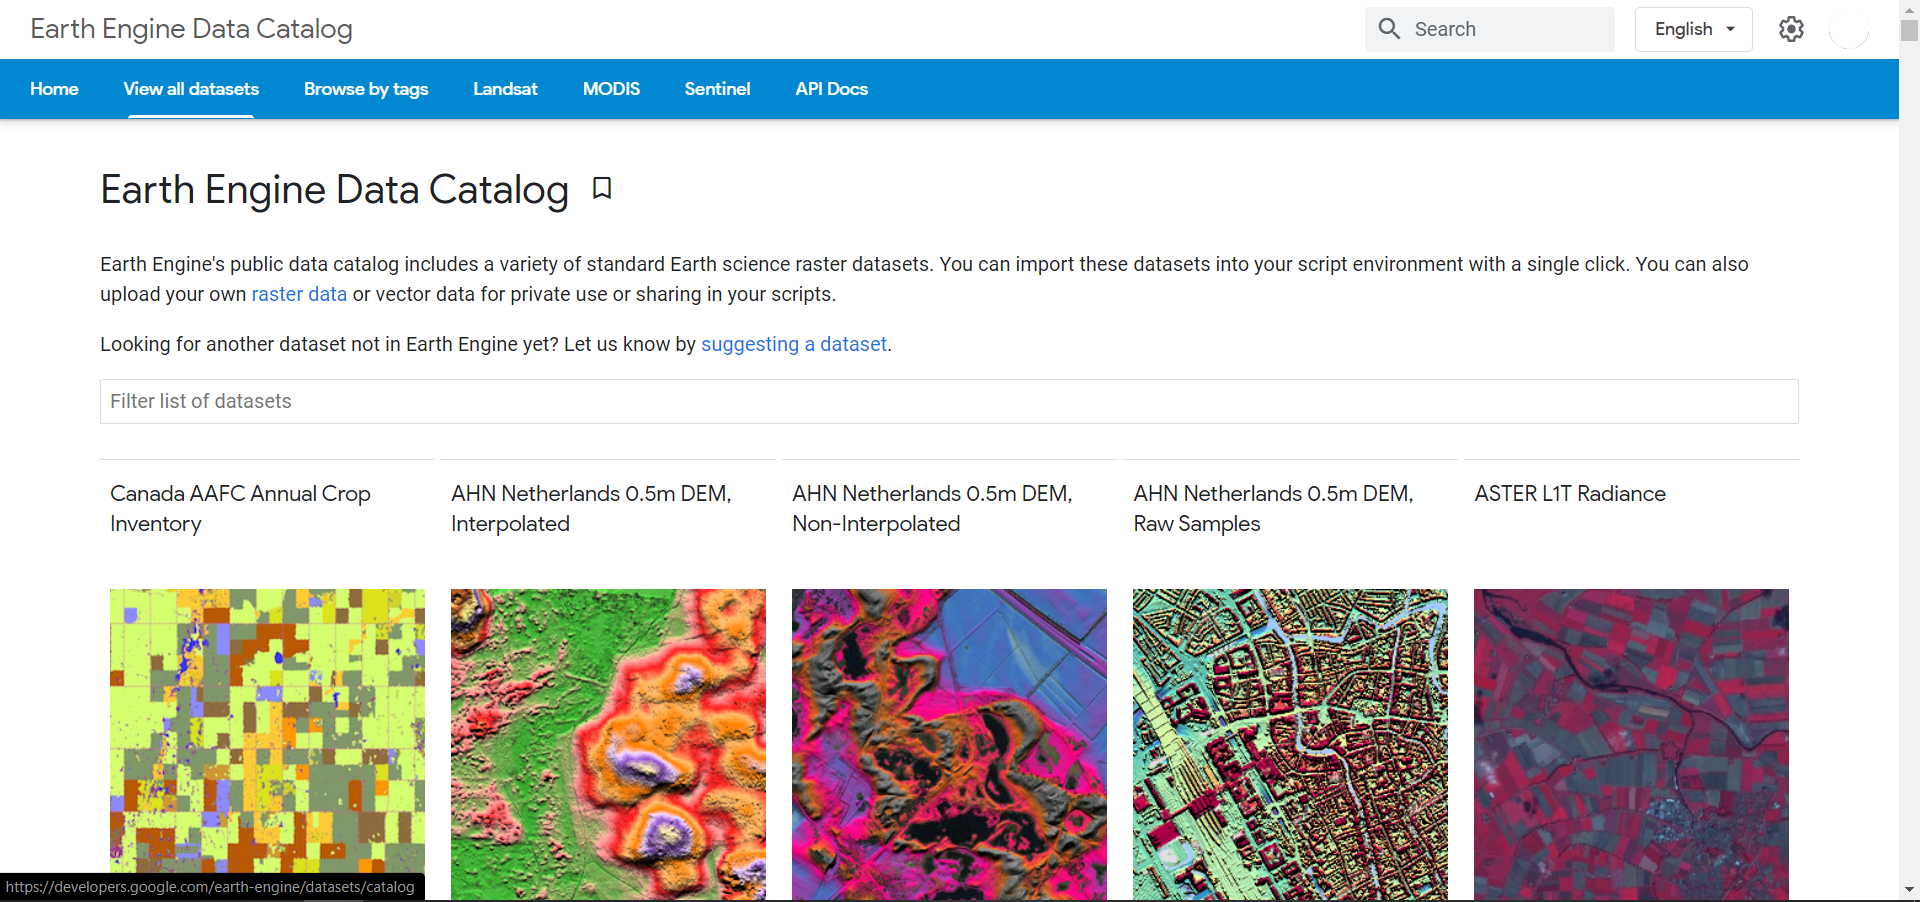
\includegraphics[width=0.95\linewidth]{Img/Datasets} 

}

\caption{Algunos ejemplos de fuentes de información disponibles en GEE.}\label{fig:f11}
\end{figure}

\begin{bluebox2}

\begin{awesomeblock}{5pt}{\faLightbulb}{darkblue}
Para consultar toda la información que está disponible en GEE se puede dirigir al siguiente enlace: \url{https://developers.google.com/earth-engine/datasets}. Se estima que en 2010 GEE era capaz de ejecutar en cuestión de días procesamientos que en un computador personal habrían tardado 15 años.

\end{awesomeblock}

\end{bluebox2}

De manera paralela al catálogo de información, GEE puso a disposición de la gente un conjunto de servidores para poder realizar rápida y eficazmente cálculos y computaciones sobre esos datos. En 2010, estos servidores tenían una capacidad más o menos equivalente a 10 000 computadores personales.

El tercer componente clave para el funcionamiento de GEE son las API. Una API es una interfaz que permite la comunicación entre nosotros (los usuarios) y los servidores de Google, proporcionando el acceso y el uso de la capacidad computacional de Google para nuestros análisis. Las API de GEE tienen el objetivo de facilitar la creación de programas, por lo cual cuentan con una serie de funciones, métodos y algoritmos preprogramados que se pueden llamar con una simple línea de código. La idea central de las API de GEE es brindar una interfaz que permita crear códigos y programas claros y concisos.

GEE ofrece dos API, una en JavaScript, a la cual se accede vía internet mediante un explorador y es la más conocida, actualizada y amigable con los usuarios. Además, es la que contiene más documentación y ayuda disponible. Por esta razón, el manual se enfocará en la API de JavaScript. Por otro lado, existe la API en Python, la cual se puede trabajar desde la consola de Python y permite ---hasta cierto punto--- usar complementariamente bibliotecas de Python, para así hacer procesamientos más complejos, o funcionalidades que la API de JavaScript no permite. Sin embargo, las desventajas de la API de Python incluyen el tener que instalar varias bibliotecas en la computadora para poder trabajar con GEE, el hecho de que existe mucho menos documentación y ayuda disponible para esta API, y que requiere de la actualización constante de algunas bibliotecas para su uso apropiado. A continuación se mencionan algunas de las principales ventajas de la API de JavaScript respecto de la de Python:

\begin{enumerate}
\def\labelenumi{\arabic{enumi}.}
\tightlist
\item
  Los datos pueden ser consultados directamente en la nube (no se requiere descargarlos para trabajar con ellos), lo que ahorra tiempo y espacio de almacenamiento para el usuario. En cambio, si se quiere usar alguna biblioteca de Python será necesario descargar la información.
\item
  El procesamiento se hace en la nube, a través de internet, utilizando el poder de cómputo asignado para la API, lo cual reduce el gasto de memoria RAM (solo necesita una conexión estable y el consumo de RAM depende del consumo del navegador). En la API de Python hay un mayor consumo de memoria RAM (para ejecutar la consola de Python y sus bibliotecas) y requiere igualmente una conexión estable a internet.
\item
  Su interfaz es mucho más amigable con los usuarios, ya que ofrece una plataforma más interactiva para programar y sencilla para enseñar.
\item
  Se pueden realizar fácilmente consultas de las colecciones de imágenes y sus metadatos antes de decidir importarlos. En cambio, la API de Python no permite realizarlas de manera tan sencilla, de modo que hay que tener una absoluta claridad de las propiedades del conjunto de datos que se van a utilizar.
\item
  Otra gran ventaja de la plataforma JavaScript radica en que los códigos se guardan en la sesión de cada usuario. Esto permite mantener un control de los códigos y automáticamente se genera un registro histórico (parecido al control de versiones de Git), lo cual facilita el seguimiento y comparación de cambios entre las versiones (y permite regresar a versiones anteriores). Además, se pueden generar repositorios compartidos para generar proyectos colaborativos.
\end{enumerate}

\begin{bluebox2}

\begin{awesomeblock}{5pt}{\faLightbulb}{darkblue}
Git es un programa de distribución libre que permite llevar un control de diferentes versiones de un código.

\end{awesomeblock}

\end{bluebox2}

\hypertarget{ejemplos-de-estudios-realizados-con-gee}{%
\subsection*{Ejemplos de estudios realizados con GEE}\label{ejemplos-de-estudios-realizados-con-gee}}
\addcontentsline{toc}{subsection}{Ejemplos de estudios realizados con GEE}

GEE se ha utilizado para diversos estudios enfocados en analizar la superficie terrestre mediante sensores remotos, especialmente imágenes multiespectrales (por ejemplo: Landsat, Sentinel-2, MODIS) y en algunos casos imágenes de radar de apertura sintética (por ejemplo, Sentinel-1). Algunos ejemplos de sus usos son:

\begin{itemize}
\tightlist
\item
  Realizar análisis de series de tiempo para detectar cambios de cobertura (Arévalo \emph{et al}., 2020; Hamunyela \emph{et al}., 2020).
\item
  Evaluar los cambios de la cobertura boscosa global para periodos superiores a una década (Hansen \emph{et al}., 2013).
\item
  Estimar variables biofísicas de la superficie terrestre (Campos-Taberner \emph{et al}., 2018).
\item
  Enmascarar nubes de imágenes (Mateo-García \emph{et al}., 2018).
\item
  Monitorear asentamientos humanos (Trianni \emph{et al}., 2014).
\item
  Analizar la disponibilidad de imágenes y observaciones despejadas (Solórzano \emph{et al}., 2020a; Solórzano \emph{et al}., 2020b).
\item
  Mapear campos de cultivo (Xiong \emph{et al}., 2017; Dong \emph{et al}., 2016).
\item
  Identificar plantaciones de palma de aceite (Lee \emph{et al}., 2016).
\item
  Mapear cicatrices de incendios (Arruda \emph{et al}., 2021).
\item
  Evaluar el grado de sequía de la superficie terrestre (Sazib \emph{et al}., 2018).
\item
  Mapear características de humedales (Slagter \emph{et al}., 2018).
\item
  Monitorear anomalías térmicas en volcanes (Genzano \emph{et al}., 2020).
\item
  Mapear agricultura protegida (Perilla \emph{et al}., 2019).
\item
  Monitorear exposición de arrecifes de coral a estresores ambientales (Williamson \emph{et al}., 2021).
\item
  Mapear plantas fotovoltáicas (Zhang \emph{et al}., 2021)
\item
  Caracterizar islas de calor (Ravanelli \emph{et al}., 2018), entre muchos otros.
\end{itemize}

Además, es una herramienta cuyo uso ha ido en aumento gracias a sus enormes capacidades de procesamiento y su rapidez para realizar análisis con información geoespacial (Kumar \emph{et al}., 2018). Por último, cabe mencionar que dentro de Google Earth Engine se pueden programar aplicaciones que facilitan el uso y consulta de resultados de cualquier código, en una interfaz amigable para cualquier usuario. Aunque esto no se revisará en el material de este manual, en la siguiente lista se pueden consultar algunos de estos ejemplos:

\begin{itemize}
\tightlist
\item
  Realizar análisis de series de tiempo para detectar cambios de cobertura (Arévalo \emph{et al}., 2020; Hamunyela \emph{et al}., 2020). \url{https://parevalo-bu.users.earthengine.app/view/advanced-tstools}, \url{https://andreim.users.earthengine.app/view/bfastmonitor}
\item
  Evaluar los cambios de la cobertura boscosa global para periodos superiores a una década (Hansen \emph{et al}., 2013). \url{https://glad.earthengine.app/view/global-forest-change}
\item
  Enmascarar nubes de imágenes (Mateo-García \emph{et al}., 2018) \url{https://isp.uv.es/projects/cdc/viewer_l8_GEE.html}
\item
  Mapear el cambio de hábitat de las aves del 2000 al 2021 (Perilla \emph{et al}., 2022) \url{https://biomodelos-iavh.users.earthengine.app/view/biomodelos}
\item
  Mapear plantas de energía fotovoltaica (paneles solares) (Zhang, \emph{et al}., 2021) \url{https://xunhezhang.users.earthengine.app/view/ningxia-pv-power-plants}
\item
  Monitorear anomalías termales volcánicas globales (Genzano, \emph{et al}., 2020) \url{https://nicogenzano.users.earthengine.app/view/nhi-tool}
\item
  Monitorear estrés ambiental para corales en el mundo (Williamson, \emph{et al}., 2021) \url{https://mjw1280.users.earthengine.app/view/coral-reef-stress-exposure-index}
\end{itemize}

\begin{bluebox2}

\begin{awesomeblock}{5pt}{\faLightbulb}{darkblue}
GEE sugiere que para citar su herramienta en cualquier tipo de trabajo se haga referencia a Gorelick \emph{et al}. (2017).

\end{awesomeblock}

\end{bluebox2}

\newpage

\hypertarget{primeros-pasos}{%
\chapter{Primeros pasos}\label{primeros-pasos}}

\hypertarget{registro-para-el-uso-de-gee-javascript-api}{%
\section{Registro para el uso de GEE JavaScript API}\label{registro-para-el-uso-de-gee-javascript-api}}

Lo primero que hay que hacer para poder utilizar la API de JavaScript de GEE es ingresar a su sitio web para registrarse como usuario, por medio del siguiente enlace:

\url{https://earthengine.google.com/}

Después, le damos clic en la esquina superior derecha donde dice \textbf{Sign Up} (inscribirse; \textcolor{darkblue}{Fig.} \ref{fig:f21}).

\begin{figure}[H]

{\centering 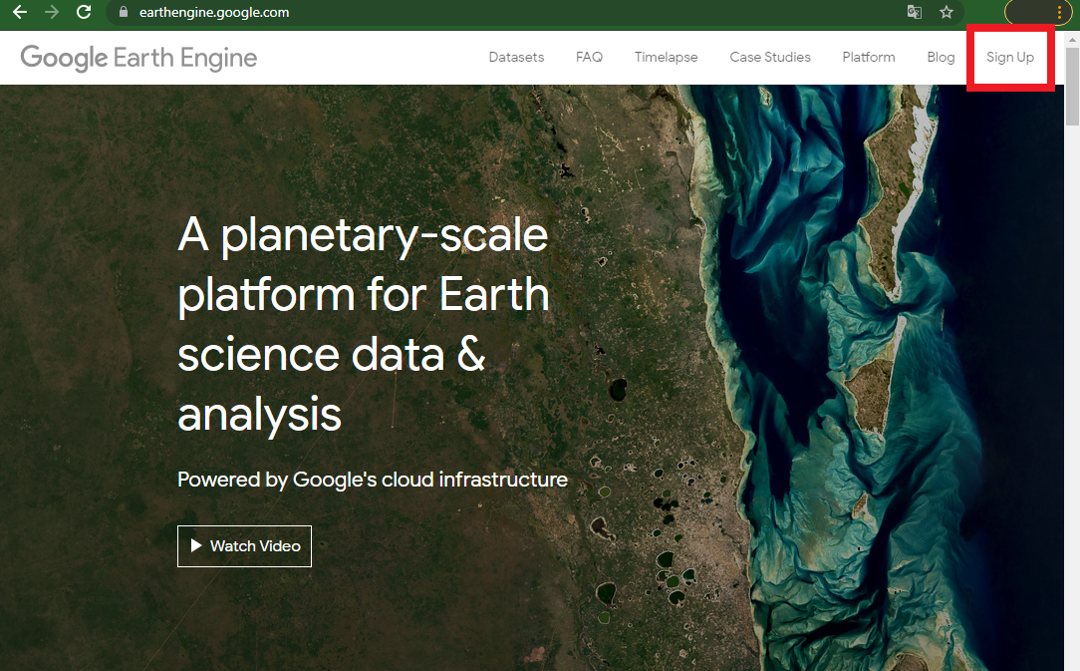
\includegraphics[width=0.8\linewidth]{Img/Signup} 

}

\caption{Pantalla de inicio en la página de registro de GEE.}\label{fig:f21}
\end{figure}

Luego se ingresan todos los datos que pide el formulario. Recuerde que para utilizar GEE se requiere de una cuenta de Google (\textcolor{darkblue}{Fig.} \ref{fig:f22}).

\begin{bluebox2}

\begin{awesomeblock}{5pt}{\faLightbulb}{darkblue}
Se recomienda usar una cuenta de Google que tenga suficiente espacio disponible en Google Drive, ya que será la forma más fácil de exportar los resultados generados en GEE.

\end{awesomeblock}

\end{bluebox2}

\begin{figure}[H]

{\centering 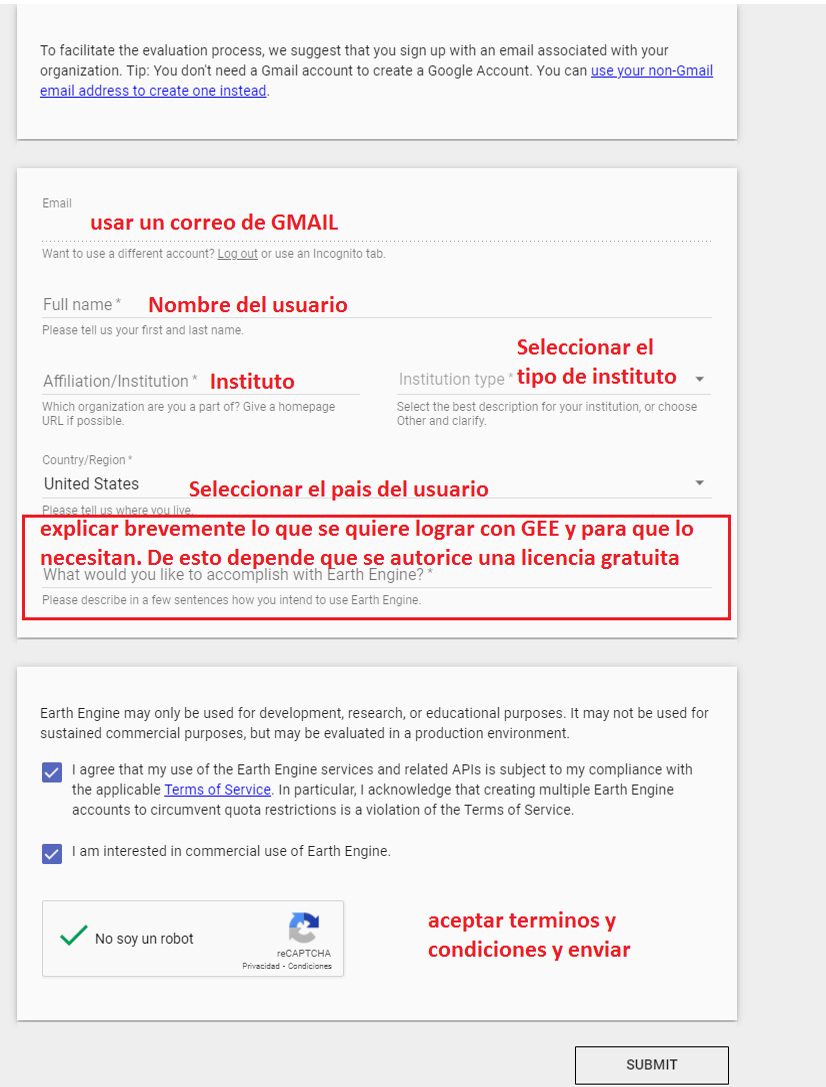
\includegraphics[width=0.8\linewidth]{Img/formulario} 

}

\caption{Formulario de datos a llenar para registrarse en GEE.}\label{fig:f22}
\end{figure}

Una vez realizado el registro, hay que esperar un tiempo (pueden ser desde minutos a días) hasta que llegue una confirmación por parte de GEE a nuestro correo informando que ya se puede hacer uso de la API (\textcolor{darkblue}{Fig.} \ref{fig:f23}).

\begin{figure}[H]

{\centering 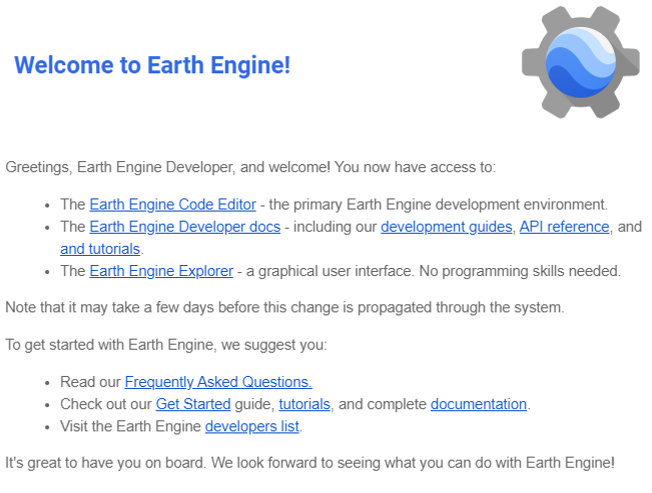
\includegraphics[width=0.6\linewidth]{Img/correo} 

}

\caption{Ejemplo del correo de confirmación por parte de GEE para poder utilizar la API.}\label{fig:f23}
\end{figure}

Una vez que tengamos dicha confirmación, podemos acceder a la API a través del siguiente enlace: \url{https://code.earthengine.google.com/}, y se accede con la cuenta de Google con la que nos registramos.

Una vez registrados, se podrá acceder al material de todos los ejercicios entrando al siguiente enlace: \url{https://code.earthengine.google.com/?accept_repo=users/JonathanVSV/GEE_manual}

\hypertarget{elementos-buxe1sicos-de-la-interfaz-gruxe1fica}{%
\section{Elementos básicos de la interfaz gráfica}\label{elementos-buxe1sicos-de-la-interfaz-gruxe1fica}}

Una vez abierta la API de JavaScript, se observan cuatro pantallas (\textcolor{darkblue}{Fig.} \ref{fig:f24}): la pantalla de repositorios, la pantalla de rutinas, la pantalla de mapa y la pantalla de control.

\begin{figure}[H]

{\centering 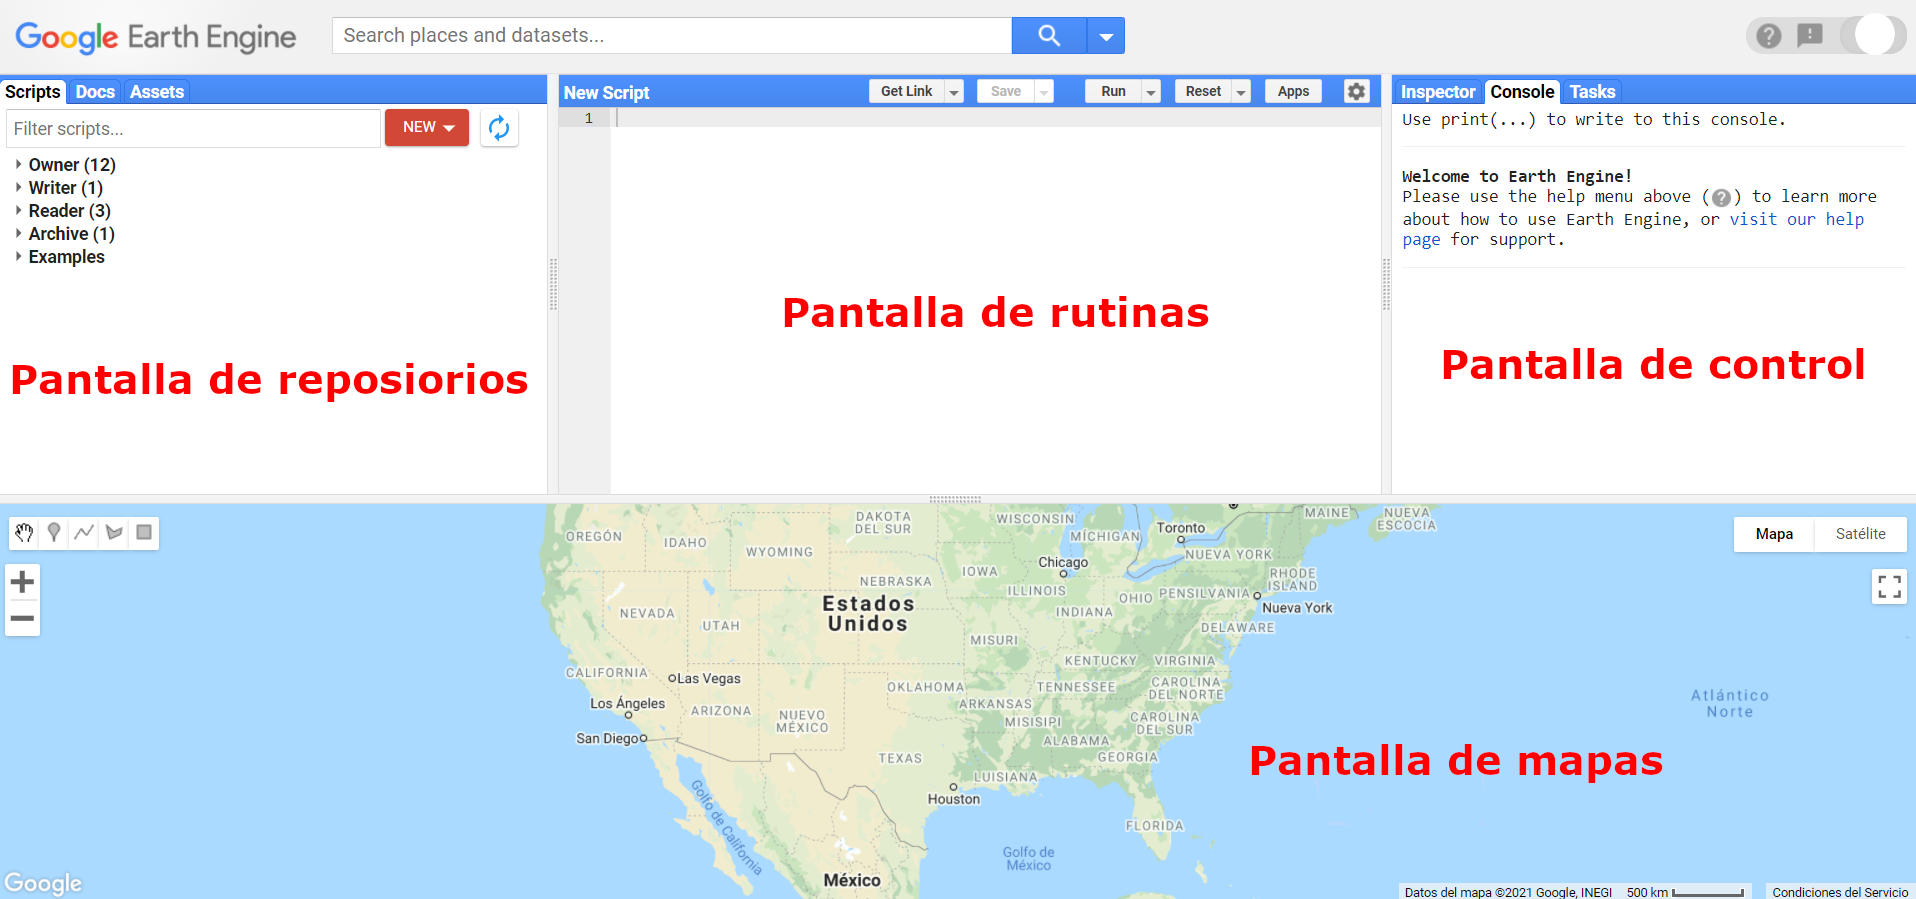
\includegraphics[width=0.95\linewidth]{Img/GEE_inicio_API2} 

}

\caption{Vista inicial de la API de GEE.}\label{fig:f24}
\end{figure}

Los elementos de la API se enlistan a continuación:

\hypertarget{pantalla-de-repositorios}{%
\subsection*{Pantalla de repositorios}\label{pantalla-de-repositorios}}
\addcontentsline{toc}{subsection}{Pantalla de repositorios}

\hypertarget{scripts}{%
\subsubsection*{Scripts}\label{scripts}}
\addcontentsline{toc}{subsubsection}{Scripts}

La pantalla de repositorios es el espacio donde se guardan y ordenan las rutinas o \emph{scripts} del usuario. En ella se pueden crear repositorios y carpetas para organizar los archivos de código, como se muestra a continuación (\textcolor{darkblue}{Fig.} \ref{fig:f25}):

\begin{figure}[H]

{\centering 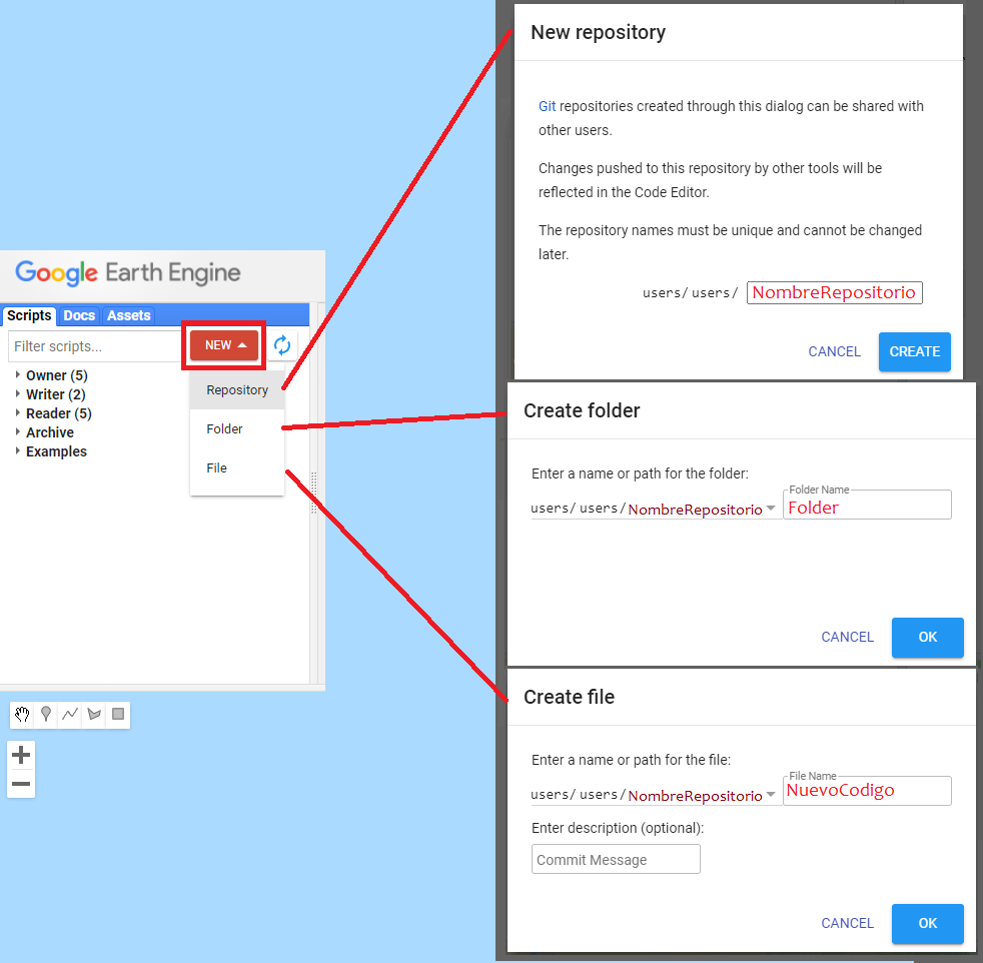
\includegraphics[width=0.8\linewidth]{Img/repofolderfile} 

}

\caption{Opciones disponibles dentro de la pestaña de Nuevo.}\label{fig:f25}
\end{figure}

Dentro de este espacio existen varias categorías. Las primeras tres se pueden utilizar para determinar distintos niveles de acceso para diversos usuarios (\textcolor{darkblue}{Fig.} \ref{fig:f26}):

\begin{figure}[H]

{\centering 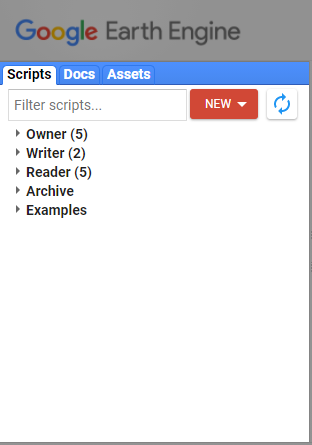
\includegraphics[width=0.6\linewidth]{Img/left_panel} 

}

\caption{Vista del panel de repositorios dentro de GEE.}\label{fig:f26}
\end{figure}

\begin{enumerate}
\def\labelenumi{\arabic{enumi}.}
\tightlist
\item
  \textbf{Owner} (Propietario): en esta sección se guardan los códigos creados por el mismo usuario.
\item
  \textbf{Writer} (Editor): en este apartado se guardan códigos que pueden ser creados por otros usuarios, pero que estamos autorizados a modificar.
\item
  \textbf{Reader} (Lector): en esta parte aparecen códigos que otros usuarios nos han compartido, pero no estamos autorizados a modificar.
\item
  \textbf{Examples} (Ejemplos): se pueden consultar ejemplos de código para hacer algunas tareas específicas. Por ejemplo, existe un apartado específico para consultar las distintas maneras de enmascarar nubes utilizando diferentes colecciones de imágenes (por ejemplo: Landsat 4-7, Landsat 8-9, Sentinel-2, MODIS).
\item
  \textbf{Archive} (Archivo): se pueden guardar archivos de código que ya no se utilicen, pero que no se desea eliminar.
\end{enumerate}

\begin{bluebox2}

\begin{awesomeblock}{5pt}{\faLightbulb}{darkblue}

El usuario puede compartir repositorios con otros usuarios de GEE como lector o editor. De esta manera, todos los archivos que se encuentren dentro de un repositorio serán compartidos con los usuarios indicados. Esta opción está disponible al dar clic en el símbolo del engranaje a la derecha de cada repositorio (aparece una vez que se coloca el puntero sobre el nombre del repositorio; \textcolor{darkblue}{Fig.} \ref{fig:f27}).

\begin{figure}[H]

{\centering 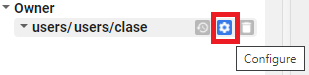
\includegraphics[width=0.6\linewidth]{Img/engranaje} 

}

\caption{Vista del espacio de propietario.}\label{fig:f27}
\end{figure}

\end{awesomeblock}

\end{bluebox2}

\hypertarget{docs}{%
\subsubsection*{Docs}\label{docs}}
\addcontentsline{toc}{subsubsection}{Docs}

Es un área donde se pueden consultar todos los métodos y algoritmos que se encuentran preprogramados y cargados en GEE (\textcolor{darkblue}{Fig.} \ref{fig:f28}). Además, para cada método se indica lo que hace, la entrada que requiere y el tipo de objeto que se obtiene como salida, así como los argumentos del método (\textcolor{darkblue}{Fig.} \ref{fig:f29}). Estos métodos se encuentran agrupados por objetos del servidor (los objetos se explican más adelante). Adicionalmente, tiene un buscador donde también se pueden consultar los métodos.

\begin{figure}[H]

{\centering 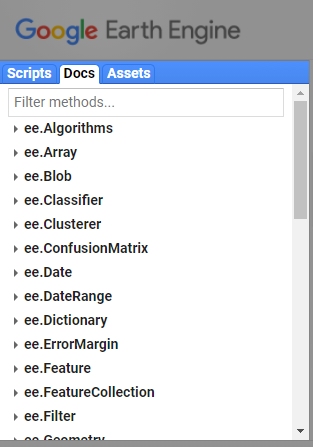
\includegraphics[width=0.6\linewidth]{Img/docs} 

}

\caption{Ejemplo de la pestaña de documentación dentro de GEE.}\label{fig:f28}
\end{figure}

\begin{figure}[H]

{\centering 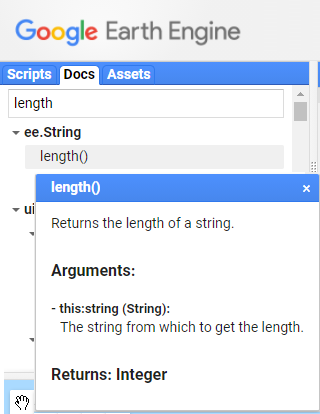
\includegraphics[width=0.6\linewidth]{Img/doc_ejemplo} 

}

\caption{Ejemplo de consulta de un método dentro de la sección de documentación.}\label{fig:f29}
\end{figure}

\hypertarget{assets}{%
\subsubsection*{Assets}\label{assets}}
\addcontentsline{toc}{subsubsection}{Assets}

La primera vez que se accede a la pestaña de \textbf{Assets} hay que crear una carpeta principal (\textbf{Home Folder}) para almacenar la información que se desee importar a GEE. Se recomienda nombrar esta carpeta con el mismo nombre de usuario (\textcolor{darkblue}{Fig.} \ref{fig:f210}).

\begin{figure}[H]

{\centering 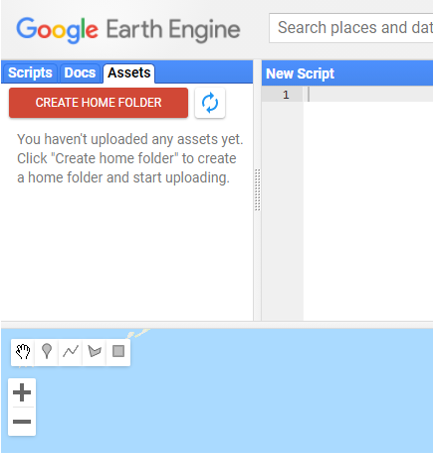
\includegraphics[width=0.6\linewidth]{Img/homeFolder} 

}

\caption{Carpeta de inicio dentro de la API.}\label{fig:f210}
\end{figure}

En este apartado el usuario puede subir y guardar su propia información para ser utilizada dentro de GEE (\textcolor{darkblue}{Fig.} \ref{fig:f211}). Se pueden subir únicamente archivos en formato ráster, vector (.shp con sus archivos auxiliares, o un .zip) o separado por comas (ver sección 4 para consultar los detalles para realizar este proceso).

\begin{figure}[H]

{\centering 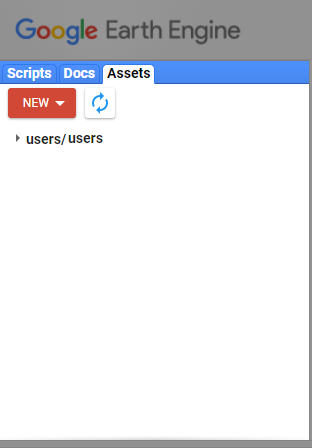
\includegraphics[width=0.6\linewidth]{Img/assets} 

}

\caption{Vista de la sección de información del usuario.}\label{fig:f211}
\end{figure}

\hypertarget{pantalla-de-rutinas}{%
\subsection*{Pantalla de rutinas}\label{pantalla-de-rutinas}}
\addcontentsline{toc}{subsection}{Pantalla de rutinas}

Esta ventana es donde se va a escribir el código en JavaScript (\textcolor{darkblue}{Fig.} \ref{fig:f212}) y cuenta con varios botones en la parte superior. El primero, \textbf{Get Link}, sirve para compartir el código que se tenga abierto mediante una liga. Además, al darle clic en la flecha de despliegue (en la opción \textbf{Manage Links}) se puede hacer un manejo de los enlaces que se tengan activos, así como borrar los que ya no se utilicen (\textcolor{darkblue}{Fig.} \ref{fig:f213}).

\begin{figure}[H]

{\centering 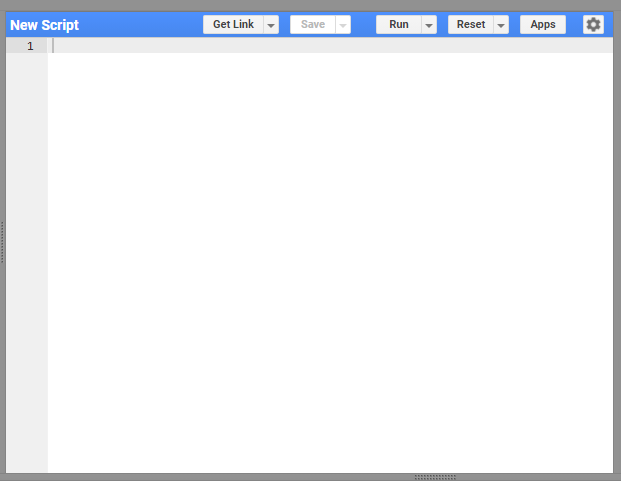
\includegraphics[width=0.7\linewidth]{Img/editor} 

}

\caption{Vista de la pantalla de rutinas o scripts.}\label{fig:f212}
\end{figure}

\begin{figure}[H]

{\centering 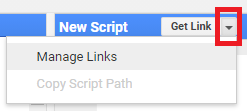
\includegraphics[width=0.5\linewidth]{Img/links} 

}

\caption{Ubicación del botón para obtener enlaces para compartir rutinas.}\label{fig:f213}
\end{figure}

A su derecha se encuentra el botón de \textbf{Save}, el cual permite guardar el código con el que se esté trabajando (\textcolor{darkblue}{Fig.} \ref{fig:f214}). Además, al darle clic en la flecha de despliegue se puede usar la opción \textbf{Save as} para crear una copia del código con otro nombre.

\begin{figure}[H]

{\centering 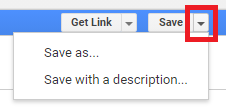
\includegraphics[width=0.5\linewidth]{Img/save} 

}

\caption{Ubicación del botón para guardar el código.}\label{fig:f214}
\end{figure}

A continuación, está el botón \textbf{Run}, que sirve para correr, de principio a fin, el código que se muestra en la pantalla de rutinas (\textcolor{darkblue}{Fig.} \ref{fig:f215}). Al darle clic a este botón se envía el código a los servidores de Google y se realiza el procedimiento indicado.

\begin{figure}[H]

{\centering 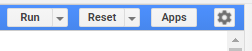
\includegraphics[width=0.5\linewidth]{Img/run} 

}

\caption{Ubicación del botón para correr el código.}\label{fig:f215}
\end{figure}

A su derecha se encuentra el botón de \textbf{Reset}, el cual sirve para borrar todo el código que se tenga escrito en la pantalla de rutinas.

Después se encuentra el botón de \textbf{Apps}, que sirve para crear aplicaciones a partir del código que se encuentra en la pantalla. La creación de aplicaciones no se cubrirá en este manual, pero se refiere a programas que permiten crear una interfaz amigable con un usuario que no tenga conocimientos de GEE. De esta manera, se puede facilitar el uso de un código programado sin necesidad de acceder directamente al código. Para consultar algunos ejemplos de aplicaciones construidas en GEE se puede visitar el siguiente enlace: \url{https://www.earthengine.app/}

Por último, en el botón del engranaje se encuentran opciones para prender y apagar líneas de código como subrayar sugerencias en la pantalla de rutinas o autocompletar símbolos como \texttt{’}, \texttt{"}, \texttt{(}, \texttt{{[}} y \texttt{\{}.

\begin{bluebox2}

\begin{awesomeblock}{5pt}{\faLightbulb}{darkblue}
Cuando se corre un código en la consola con el botón de \textbf{Run}, este no corre directamente en los servidores de Google, sino que se transcriben a código GeoJSON, se envían a los servidores de Google y se espera una respuesta.
Para buscar un texto específico dentro del código, se debe dar clic en la pantalla de rutinas y presionar ctrl+F (algunos atajos pueden variar según la configuración del teclado). Esta pantalla permite buscar una cadena de caracteres determinada dentro del código. Además, al volver a presionar ctrl+F, también se activa el recuadro de sustitución, el cual facilita el sustituir una cadena de caracteres determinada por otra. Para consultar el listado completo de atajos se puede presionar ctrl+shift+H.

\end{awesomeblock}

\end{bluebox2}

\hypertarget{search}{%
\subsection*{Search}\label{search}}
\addcontentsline{toc}{subsection}{Search}

Es una barra de búsqueda (\textbf{Search}) en la que se puede tratar de localizar fuentes de datos o sitios (\textcolor{darkblue}{Fig.} \ref{fig:f216}). Resulta útil para encontrar la ruta de alguna fuente de datos o una colección en particular, así como para consultar sus metadatos, bandas y características.

\begin{figure}[H]

{\centering 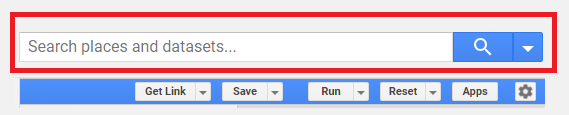
\includegraphics[width=0.8\linewidth]{Img/search} 

}

\caption{Vista de la barra de búsqueda.}\label{fig:f216}
\end{figure}

\hypertarget{pantalla-de-mapa}{%
\subsection*{Pantalla de Mapa}\label{pantalla-de-mapa}}
\addcontentsline{toc}{subsection}{Pantalla de Mapa}

En esta pantalla (\textcolor{darkblue}{Fig.} \ref{fig:f217}) se puede:

\begin{enumerate}
\def\labelenumi{\arabic{enumi}.}
\tightlist
\item
  Dibujar y visualizar puntos, polígonos, líneas o rectángulos.
\item
  Mostrar la información que se haya indicado mediante la función \boldpurple{Map.addLayer}.
\item
  Añadir un mapa base (Google Maps o Google Earth).
\end{enumerate}

\begin{figure}[H]

{\centering 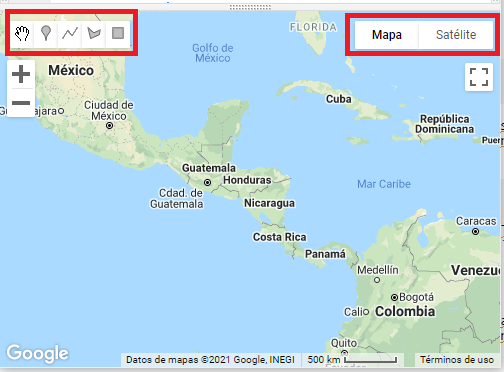
\includegraphics[width=0.95\linewidth]{Img/drawing} 

}

\caption{Vista de la pantalla de mapa, indicando las diferentes herramientas que se pueden utilizar en ella.}\label{fig:f217}
\end{figure}

\hypertarget{gestor-de-capas}{%
\subsubsection*{Gestor de capas}\label{gestor-de-capas}}
\addcontentsline{toc}{subsubsection}{Gestor de capas}

El gestor de capas permite prender y apagar las capas que se estén mostrando en el área del mapa (\textcolor{darkblue}{Fig.} \ref{fig:f218}). Además, sirve para modificar las características de su visualización (por ejemplo, transparencia, color, distribución del histograma, compuesto de color). Este menú aparece una vez que se cargan capas a la pantalla de mapa.

\begin{figure}[H]

{\centering 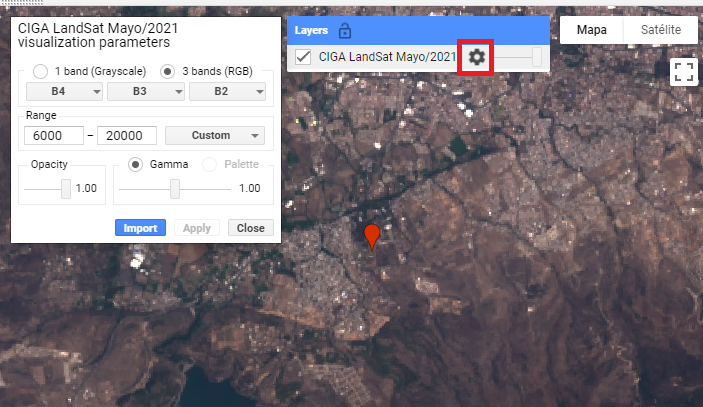
\includegraphics[width=0.95\linewidth]{Img/layer} 

}

\caption{Ejemplo del uso del administrador de capas.}\label{fig:f218}
\end{figure}

\hypertarget{pantalla-de-control}{%
\subsection*{Pantalla de control}\label{pantalla-de-control}}
\addcontentsline{toc}{subsection}{Pantalla de control}

La pantalla de control contiene tres pestañas: \textbf{Console} (consola), \textbf{Inspector} (inspector) y \textbf{Tasks} (tareas). Esta pantalla le permite al usuario hacer algunas consultas sobre la información con la que se está trabajando o finalizar tareas de exportación de información. A continuación se describe cada una de estas pestañas.

\hypertarget{console}{%
\subsubsection*{Console}\label{console}}
\addcontentsline{toc}{subsubsection}{Console}

La consola consiste en la pantalla de comunicación con el servidor (\textcolor{darkblue}{Fig.} \ref{fig:f219}). En ella se muestran los errores que se obtienen al correr un código o se puede mostrar la información indicada por la función \boldpurple{print}.

\begin{figure}[H]

{\centering 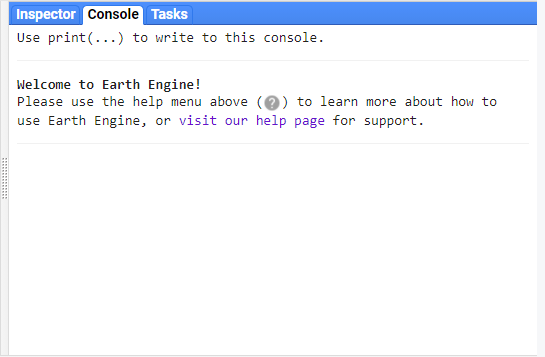
\includegraphics[width=0.8\linewidth]{Img/rigthPanel} 

}

\caption{Vista de la consola en GEE.}\label{fig:f219}
\end{figure}

\hypertarget{inspector}{%
\subsubsection*{Inspector}\label{inspector}}
\addcontentsline{toc}{subsubsection}{Inspector}

Permite consultar los valores de las capas que se muestran en el mapa, al dar clic sobre el punto de interés (\textcolor{darkblue}{Fig.} \ref{fig:f220}).

\begin{figure}[H]

{\centering 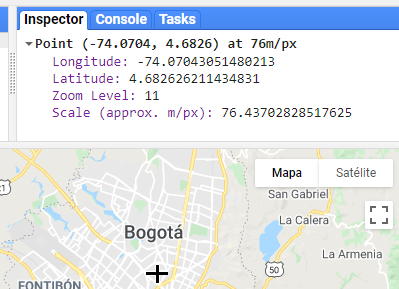
\includegraphics[width=0.95\linewidth]{Img/inspector} 

}

\caption{Vista de la pestaña de la herramienta de Inspector.}\label{fig:f220}
\end{figure}

\hypertarget{tasks}{%
\subsubsection*{Tasks}\label{tasks}}
\addcontentsline{toc}{subsubsection}{Tasks}

En esta pestaña se muestran las tareas que se hayan exportado mediante la función \boldpurple{Export} y permite correr el trabajo de exportación al sitio donde el usuario le haya indicado (drive, assets; \textcolor{darkblue}{Fig.} \ref{fig:f221}). Además, esta pestaña tiene otras funcionalidades:

\begin{enumerate}
\def\labelenumi{\arabic{enumi}.}
\tightlist
\item
  Mostrar las tareas para ejecutar (con el botón de \textbf{Run}, el cual permite especificar detalles de la exportación).
\item
  Presentar las tareas en ejecución (color gris).
\item
  Señalar el tiempo que tomó realizar en el trabajo.
\item
  Indicar cuándo se ha finalizado algún trabajo (color azul).
\item
  Cuando hay un error en algún objeto exportado, se verá el trabajo marcado en rojo. Por último, al dar clic sobre el signo de interrogación que aparece al colocar el cursor sobre algún trabajo, se puede obtener mayor información sobre este, como la ubicación del archivo exportado o más información sobre el error que arrojó el servidor al tratar de realizar una exportación.
\end{enumerate}

\begin{figure}[H]

{\centering 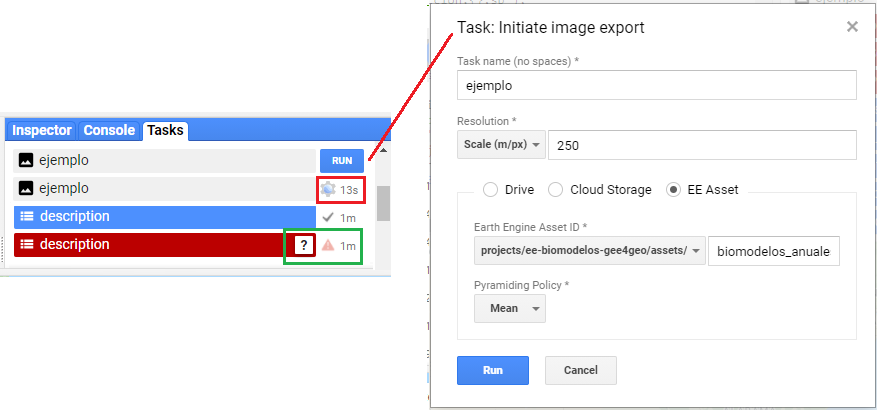
\includegraphics[width=0.95\linewidth]{Img/task} 

}

\caption{Vista de la pestaña de tareas dentro de GEE.}\label{fig:f221}
\end{figure}

\hypertarget{programaciuxf3n-en-gee}{%
\section{Programación en GEE}\label{programaciuxf3n-en-gee}}

En la API de GEE, la programación sigue la sintaxis del lenguaje JavaScript y es orientada a objetos. Estos objetos se pueden interpretar como contenedores de información sobre los que se van a aplicar diferentes funciones o métodos para crear nuevos objetos o sobrescribir objetos preexistentes. Cada tipo de objeto tiene una serie de métodos propios que le permiten realizar diferentes tipos de operaciones, los cuales se revisan en el capítulo 5.

\hypertarget{simbologuxeda}{%
\subsection*{Simbología}\label{simbologuxeda}}
\addcontentsline{toc}{subsection}{Simbología}

\begin{itemize}
\tightlist
\item
  \texttt{‘\ ’} : comillas simples.
\item
  \texttt{“\ ”} : comillas dobles.
\item
  \texttt{{[}\ {]}} : corchetes.
\item
  \texttt{\{\ \}} : llaves.
\item
  \texttt{(\ )} : paréntesis.
\item
  \texttt{-} : guion.
\item
  \texttt{\_} : guion bajo.
\item
  \texttt{,} : coma.
\end{itemize}

\hypertarget{lenguaje-javascript-en-gee}{%
\subsection*{Lenguaje JavaScript en GEE}\label{lenguaje-javascript-en-gee}}
\addcontentsline{toc}{subsection}{Lenguaje JavaScript en GEE}

La sintaxis de JavaScript tiene algunas peculiaridades que deben cumplirse para que se pueda correr el código sin problemas. Entre la sintaxis básica se pueden considerar los siguientes puntos (de igual forma iremos tocando la gramática del código a lo largo de los ejemplos):

\begin{enumerate}
\def\labelenumi{\arabic{enumi}.}
\tightlist
\item
  Es un lenguaje sensible a las mayúsculas y minúsculas, de tal manera que puede haber dos objetos diferentes, uno llamado \texttt{a} y otro llamado \texttt{A}.
\item
  Se recomienda cerrar cualquier comando con un \texttt{;} (de no hacerlo, el código funcionará igualmente; sin embargo, se recomienda utilizarlo para tener un código más claro y ordenado).
\item
  Comúnmente en JavaScript se utiliza la notación \emph{lowerCamelCase} para unir palabras (unir palabras sin espacio, pero cada una comenzando con su respectiva mayúscula), en lugar de guiones \texttt{-} o guion bajo \texttt{\_}. Por ejemplo: \boldpurple{intervalMean} o \boldpurple{updateMask}.
\item
  Todas las variables, funciones y objetos deben ser definidos mediante la función \texttt{var}. Para los usuarios de JavaScript, hay que destacar que Google Earth Engine no utiliza la función \texttt{const} para definir variables.
\item
  El operador \texttt{=} asigna un valor a una variable.
\item
  Los operadores matemáticos son: \texttt{+\ -\ *\ /}.
\item
  Para concatenar dos cadenas de caracteres se utiliza el símbolo \texttt{+}.
\item
  Para realizar comentarios se puede utilizar \texttt{//} para comentarios de una línea, o también \texttt{/*\ …\ */} para comentarios de varias líneas.
\item
  Se suele utilizar el operador \texttt{.} (punto) para aplicar un método al objeto que lo precede. En este manual, todos los métodos aplicados a algún objeto se escribirán precedidos por el operador \texttt{.} para evitar errores de sintaxis.
\item
  Son igualmente válidas tanto las comillas sencillas (\texttt{\textquotesingle{}\ \textquotesingle{}}) como las comillas dobles (\texttt{"\ """}), pero no deben mezclarse ambos tipos de comillas en una misma línea.
\end{enumerate}

\begin{bluebox2}

\begin{awesomeblock}{5pt}{\faLightbulb}{darkblue}
El término correcto para llamar a los procesos aplicados con el operador \texttt{.} es el de método (\emph{method}), lo cual quiere decir que son procedimientos ligados a un tipo de objeto. Por ejemplo, en \boldpurple{ee.Image.updateMask}, el método \boldpurple{updateMask} es uno ligado a un objeto de tipo imagen (\boldpurple{ee.Image}). Por el contrario, las funciones en un sentido estricto se aplican a un objeto mediante la sintaxis: \texttt{function(objeto)\{\}}. Distintos tipos de objetos tienen diferentes métodos ligados a ellos.

\end{awesomeblock}

\end{bluebox2}

\newpage

\hypertarget{interfaz-de-usuario}{%
\chapter{Interfaz de usuario}\label{interfaz-de-usuario}}

Dentro de GEE hay un grupo de funciones que permiten interactuar con los objetos, y obtener información sobre sus características o propiedades, y visualizarlos o exportarlos para trabajar con ellos en un entorno distinto a GEE. A este conjunto de funciones le llamaremos funciones de interfaz de usuario. Estas funciones resultan muy útiles para ayudar al usuario a entender los procesos que está programando, así como para verificar que los procesos realicen la tarea deseada. Dentro de este grupo de funciones se distinguen, a continuación, cuatro grupos de funciones.

\hypertarget{impresiuxf3n-en-consola}{%
\section{Impresión en consola}\label{impresiuxf3n-en-consola}}

\index{print}
La función más sencilla de la interfaz es la de imprimir objetos en la consola, lo cual se realiza mediante la función \boldpurple{print} (imprimir). Al llamar esta función e indicar cualquier objeto como argumento, este se evalúa y se imprime su estructura en la consola. Esta función permite obtener información básica de los objetos como el tipo de objeto, número de registros, características y propiedades de los elementos que lo conforman. Además, esta función resulta muy útil para rastrear errores de programación (\emph{bugs}) en los códigos. El resultado de la siguiente línea de código se puede apreciar en la \textcolor{darkblue}{Fig.} \ref{fig:f31}.

\begin{Shaded}
\begin{Highlighting}[]
\FunctionTok{print}\NormalTok{(}\StringTok{\textquotesingle{}Hola Mundo\textquotesingle{}}\NormalTok{)}\OperatorTok{;}
\end{Highlighting}
\end{Shaded}

\begin{figure}[H]

{\centering 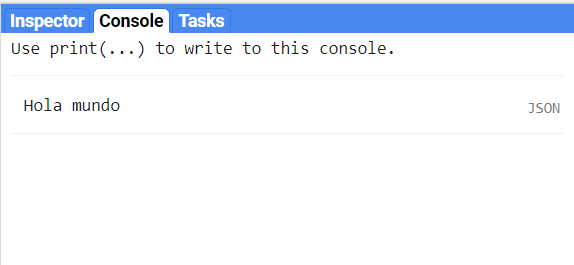
\includegraphics[width=0.8\linewidth]{Img/holaMundo} 

}

\caption{Ejemplo del uso de la función print para imprimir en la consola.}\label{fig:f31}
\end{figure}

\begin{bluebox2}

\begin{awesomeblock}{5pt}{\faLightbulb}{darkblue}
Se recomienda utilizar varias impresiones en la consola (mediante \boldpurple{print}), por programa, para verificar el resultado de procesos intermedios.

\end{awesomeblock}

\end{bluebox2}

\hypertarget{interacciuxf3n-con-la-pantalla-de-mapa}{%
\section{Interacción con la pantalla de mapa}\label{interacciuxf3n-con-la-pantalla-de-mapa}}

Este grupo de funciones permiten agregar objetos del lado del servidor a la pantalla de mapa, así como controlar algunos parámetros de dicha pantalla. Todas las funciones encargadas del manejo de la pantalla de mapa se encuentran dentro de la biblioteca \boldpurple{Map}.

\begin{bluebox2}

\begin{awesomeblock}{5pt}{\faLightbulb}{darkblue}
Para revisar todas las funciones disponibles para la interfaz del usuario, ver la sección de \textbf{Code Editor} en la siguiente liga: \url{https://developers.google.com/earth-engine/apidocs}. Además, en esta sección se indican los argumentos que acepta cada función, así como el tipo de objeto de la salida.

\end{awesomeblock}

\end{bluebox2}

\hypertarget{map.addlayer}{%
\subsubsection*{Map.addLayer}\label{map.addlayer}}
\addcontentsline{toc}{subsubsection}{Map.addLayer}

\index{Map.addLayer}
\boldpurple{Map.addLayer} permite mostrar elementos en la pantalla de mapa de la API. Por lo tanto, permite mostrar objetos de tipo vector (\boldpurple{ee.Feature}) o imagen (\boldpurple{ee.Image}; estos objetos se presentan con mayor detalle más adelante). Los argumentos de la función \boldpurple{Map.addLayer} incluyen el objeto a añadir a la pantalla de mapa, seguido de un diccionario con información para el despliegue de la capa. Por último, se puede indicar el nombre de la capa con el que se desea mostrar la capa en la pantalla de mapa.

Al utilizar \boldpurple{Map.addLayer} sobre una imagen se pueden indicar los siguientes argumentos: \texttt{bands} (bandas), \texttt{min} y \texttt{max} (valores mínimos y máximos para visualizar la información). Estos se deben pasar dentro de un par de llaves \texttt{\{\}} como un diccionario (ver Capítulo 5 para una descripción de lo que es un diccionario). La función ofrece la opción de visualizar en modo monobanda o en compuesto RGB (del inglés Red, Green, Blue). En el caso de optar por el primero, permite asignar colores mediante el argumento de palette (paleta de colores); mientras que en el segundo se deben agregar las bandas en orden, es decir, primero la banda que corresponde al canal rojo, seguida del verde y del azul (\textcolor{darkblue}{Fig.} \ref{fig:f32}).

\begin{Shaded}
\begin{Highlighting}[]
\KeywordTok{Map}\OperatorTok{.}\FunctionTok{addLayer}\NormalTok{(image}\OperatorTok{,}\NormalTok{ \{}\DataTypeTok{bands}\OperatorTok{:}\NormalTok{ [}\StringTok{\textquotesingle{}B4\textquotesingle{}}\OperatorTok{,} \StringTok{\textquotesingle{}B3\textquotesingle{}}\OperatorTok{,} \StringTok{\textquotesingle{}B2\textquotesingle{}}\NormalTok{]}\OperatorTok{,} 
                      \DataTypeTok{min}\OperatorTok{:} \DecValTok{0}\OperatorTok{,} \DataTypeTok{max}\OperatorTok{:} \DecValTok{2000}\NormalTok{\}}\OperatorTok{,} 
                      \StringTok{\textquotesingle{}RGB\textquotesingle{}}\NormalTok{)}\OperatorTok{;}
\end{Highlighting}
\end{Shaded}

\begin{figure}[H]

{\centering 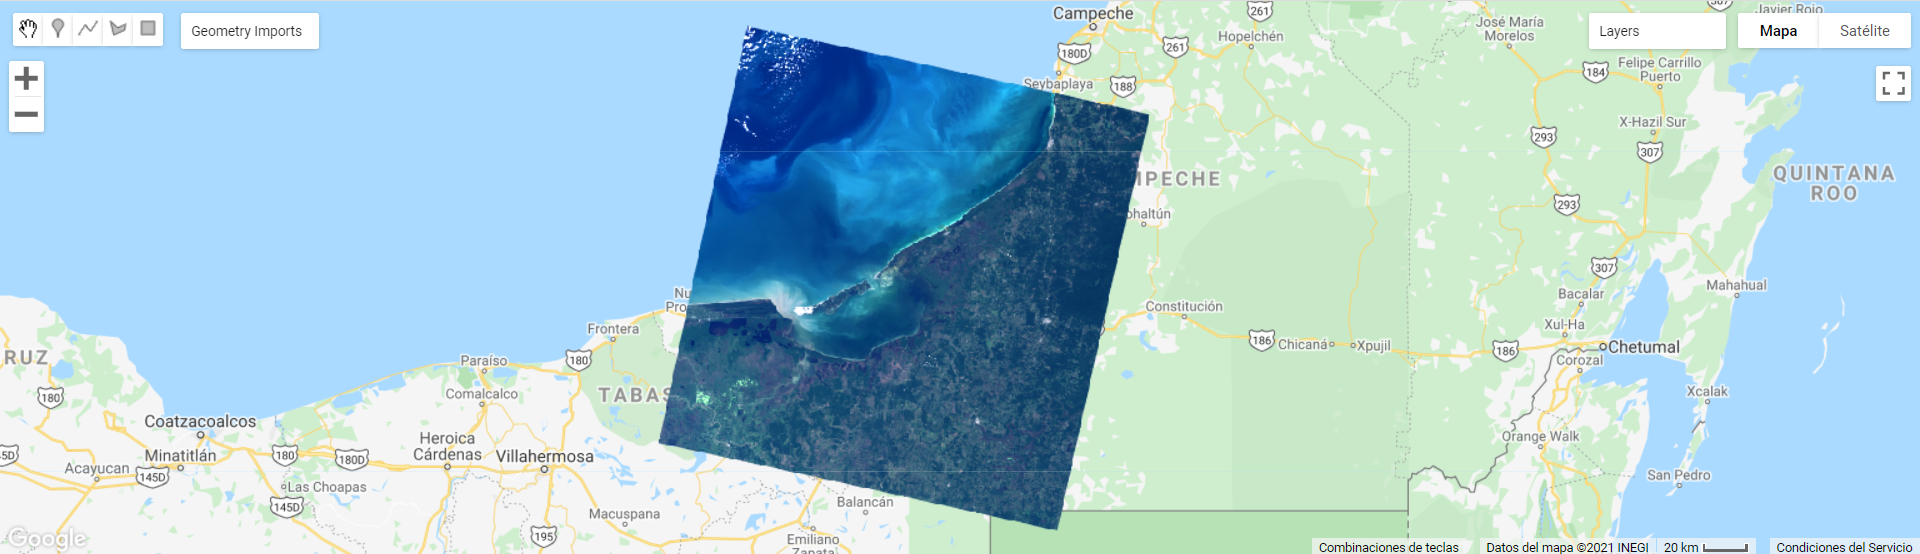
\includegraphics[width=0.95\linewidth]{Img/LTerminos} 

}

\caption{Ejemplo de visualización de un compuesto RGB de una imagen Landsat 8 sobre Laguna de Términos, México.}\label{fig:f32}
\end{figure}

\begin{bluebox2}

\begin{awesomeblock}{5pt}{\faLightbulb}{darkblue}
En algunas ocasiones, al intentar cargar objetos en la pantalla de mapa, que sean producto de procesamientos demandantes, la consola puede mostrar un error indicando que se superó el tiempo de espera o el límite de memoria disponible. En estos casos, se sugiere exportar el resultado en lugar de tratar de cargarlo en la pantalla de mapa y después visualizarlo de manera local en algún SIG o \emph{software} similar (por ejemplo, QGIS).
La proyección por defecto para mostrar la información en la pantalla de mapa corresponde a EPSG:3857. Los códigos EPSG se pueden consultar en el siguiente enlace: \url{https://epsg.io/}. Dicha proyección únicamente se hace para poder visualizar la información, mas no transforma la información con la que el usuario trabaja.

\end{awesomeblock}

\end{bluebox2}

Para el caso de los vectores (\boldpurple{ee.Feature}) se puede realizar una operación similar a las imágenes, aunque el único argumento válido es \texttt{color} (\textcolor{darkblue}{Fig.} \ref{fig:f33}):

\begin{Shaded}
\begin{Highlighting}[]
\KeywordTok{Map}\OperatorTok{.}\FunctionTok{addLayer}\NormalTok{(feature}\OperatorTok{,}\NormalTok{ \{}\DataTypeTok{color}\OperatorTok{:} \StringTok{\textquotesingle{}FF0000\textquotesingle{}}\NormalTok{\}}\OperatorTok{,} \StringTok{\textquotesingle{}featuresColored\textquotesingle{}}\NormalTok{)}\OperatorTok{;}
\end{Highlighting}
\end{Shaded}

\begin{figure}[H]

{\centering 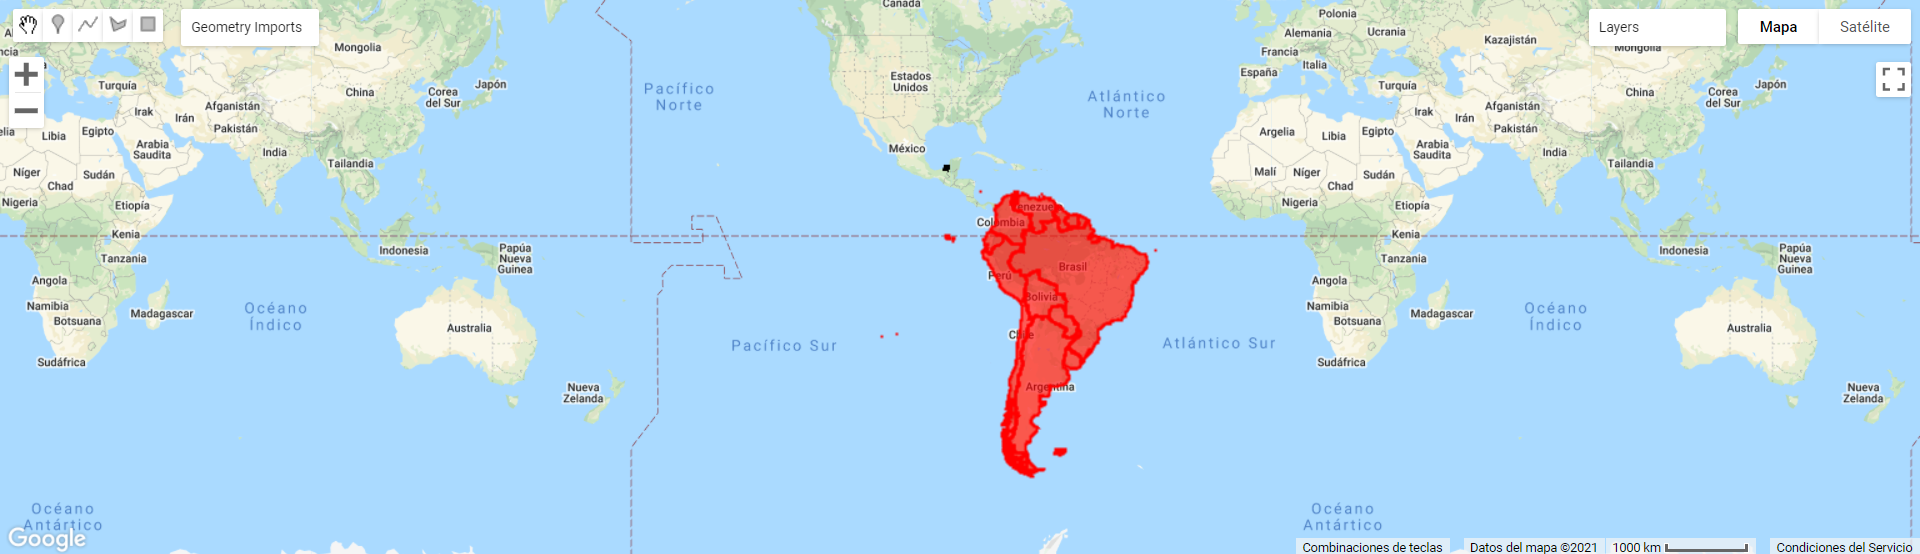
\includegraphics[width=0.95\linewidth]{Img/SAmerica} 

}

\caption{Ejemplo de visualización de un vector con los límites políticos de los países de Sudamérica donde se indica su color.}\label{fig:f33}
\end{figure}

\begin{bluebox2}

\begin{awesomeblock}{5pt}{\faLightbulb}{darkblue}
El código de los colores pasados al argumento de \texttt{palette} o \texttt{color} corresponden a códigos hexadecimales. Estos pueden ser consultados en el siguiente enlace: \url{https://htmlcolorcodes.com/es/}

\end{awesomeblock}

\end{bluebox2}

\hypertarget{map.centerobject}{%
\subsubsection*{Map.centerObject}\label{map.centerobject}}
\addcontentsline{toc}{subsubsection}{Map.centerObject}

\index{Map.centerObject}
Esta función permite centrar la pantalla de mapa en algún objeto o coordenada (longitud, latitud). Además, se puede indicar el zoom con el cual se quiere centrar el objeto.

\begin{Shaded}
\begin{Highlighting}[]
\KeywordTok{Map}\OperatorTok{.}\FunctionTok{setCenter}\NormalTok{(}\OperatorTok{{-}}\FloatTok{39.86}\OperatorTok{,} \FloatTok{20.52}\OperatorTok{,} \DecValTok{5}\NormalTok{)}
\end{Highlighting}
\end{Shaded}

\hypertarget{creaciuxf3n-de-gruxe1ficos}{%
\section{Creación de gráficos}\label{creaciuxf3n-de-gruxe1ficos}}

Este grupo de funciones permiten realizar gráficos de diversos tipos; sin embargo, cada tipo de gráfico contiene argumentos válidos diferentes. Todas estas funciones se encuentran agrupadas dentro de la biblioteca \boldpurple{ui.Chart}. Los objetos básicos que permite graficar GEE son: vectores (\boldpurple{ee.Feature}), colecciones de vectores (\boldpurple{ee.FeatureCollection}), imágenes (\boldpurple{ee.Image}), colecciones de imágenes (\boldpurple{ee.ImageCollection}), arreglos (\boldpurple{ee.Array}) y listas (\boldpurple{ee.List}). Además, para indicar los colores a utilizar en el gráfico o el título del mismo se puede utilizar el método \boldpurple{.setOptions} sobre el objeto de tipo gráfico.

\hypertarget{ui.chart.feature}{%
\subsubsection*{ui.Chart.feature}\label{ui.chart.feature}}
\addcontentsline{toc}{subsubsection}{ui.Chart.feature}

\index{ui.Chart.feature}
Este conjunto de funciones permite obtener distintos tipos de gráficos a partir de un vector o una colección de vectores y mostrar su resultado al imprimirlos en la consola (mediante la función \boldpurple{print}). Algunas de las funciones disponibles son:

\begin{itemize}
\tightlist
\item
  \boldpurple{ui.Chart.feature.byFeature}.
\item
  \boldpurple{ui.Chart.feature.byProperty}.
\item
  \boldpurple{ui.Chart.feature.groups}.
\item
  \boldpurple{ui.Chart.feature.histogram}.
\end{itemize}

Por ejemplo:

\begin{Shaded}
\begin{Highlighting}[]
\KeywordTok{ui}\OperatorTok{.}\AttributeTok{Chart}\OperatorTok{.}\AttributeTok{feature}\OperatorTok{.}\FunctionTok{byProperty}\NormalTok{(\{}
  \CommentTok{// Indicar el vector o colección de atributos a partir del cual se }
  \CommentTok{// va a hacer el gráfico}
  \DataTypeTok{feature}\OperatorTok{:}\NormalTok{ coleccionAtributos}\OperatorTok{,} 
  \CommentTok{// La propiedad a colocar en el eje de las x}
  \DataTypeTok{xProperties}\OperatorTok{:} \StringTok{\textquotesingle{}Clase\textquotesingle{}}\OperatorTok{,}
\NormalTok{\})}
\end{Highlighting}
\end{Shaded}

\hypertarget{ui.chart.image}{%
\subsubsection*{ui.Chart.image}\label{ui.chart.image}}
\addcontentsline{toc}{subsubsection}{ui.Chart.image}

\index{ui.Chart.image}
Este conjunto de funciones permite obtener distintos tipos de gráficos a partir de una imagen o colección de imágenes. Algunas de las funciones que se encuentran disponibles son:

\begin{itemize}
\tightlist
\item
  \boldpurple{ui.Chart.image.byClass}.
\item
  \boldpurple{ui.Chart.image.byRegion}.
\item
  \boldpurple{ui.Chart.image.doySeries}.
\item
  \boldpurple{ui.Chart.image.histogram}.
\item
  \boldpurple{ui.Chart.image.seriesByRegion}.
\end{itemize}

Por ejemplo, para graficar una serie de tiempo a partir de una colección de imágenes se utiliza la función \boldpurple{ui.Chart.image.seriesByRegion} (\textcolor{darkblue}{Fig.} \ref{fig:f34}).

\begin{Shaded}
\begin{Highlighting}[]
\KeywordTok{ui}\OperatorTok{.}\AttributeTok{Chart}\OperatorTok{.}\AttributeTok{image}\OperatorTok{.}\FunctionTok{seriesByRegion}\NormalTok{(\{}
  \CommentTok{// Definir la colección de imágenes a graficar}
  \DataTypeTok{imageCollection}\OperatorTok{:}\NormalTok{ coleccionImagenes}\OperatorTok{,} 
  \CommentTok{// Definir las regiones sobre las cuales se va a extraer la}
  \CommentTok{// información para el gráfico}
  \DataTypeTok{regions}\OperatorTok{:}\NormalTok{ areas}\OperatorTok{.}\FunctionTok{filter}\NormalTok{(}\KeywordTok{ee}\OperatorTok{.}\AttributeTok{Filter}\OperatorTok{.}\FunctionTok{eq}\NormalTok{(}\StringTok{\textquotesingle{}Tipo\textquotesingle{}}\OperatorTok{,}\StringTok{\textquotesingle{}Bosque\textquotesingle{}}\NormalTok{))}\OperatorTok{,}
  \CommentTok{// El reductor a utilizar para resumir la información de la}
  \CommentTok{// colección de imágenes en las regiones indicadas}
  \DataTypeTok{reducer}\OperatorTok{:} \KeywordTok{ee}\OperatorTok{.}\AttributeTok{Reducer}\OperatorTok{.}\FunctionTok{mean}\NormalTok{()}\OperatorTok{,} 
  \CommentTok{// La banda sobre la cual se quiere construir el gráfico}
  \DataTypeTok{band}\OperatorTok{:} \StringTok{\textquotesingle{}NDVI\textquotesingle{}}\OperatorTok{,} 
  \CommentTok{// Tamaño en m del píxel para obtener la información}
  \DataTypeTok{scale}\OperatorTok{:} \DecValTok{30}\OperatorTok{,} 
  \CommentTok{// Propiedad para nombrar a cada serie}
  \DataTypeTok{seriesProperty}\OperatorTok{:} \StringTok{\textquotesingle{}Tipo\textquotesingle{}}
\NormalTok{\})}
  \OperatorTok{.}\FunctionTok{setOptions}\NormalTok{(\{}
    \DataTypeTok{title}\OperatorTok{:} \StringTok{\textquotesingle{}Bosque\textquotesingle{}}\OperatorTok{,}
    \DataTypeTok{colors}\OperatorTok{:}\NormalTok{ [}\StringTok{\textquotesingle{}\#EE3A19\textquotesingle{}}\NormalTok{]}
\NormalTok{  \})}\OperatorTok{;}
\end{Highlighting}
\end{Shaded}

\begin{figure}[H]

{\centering 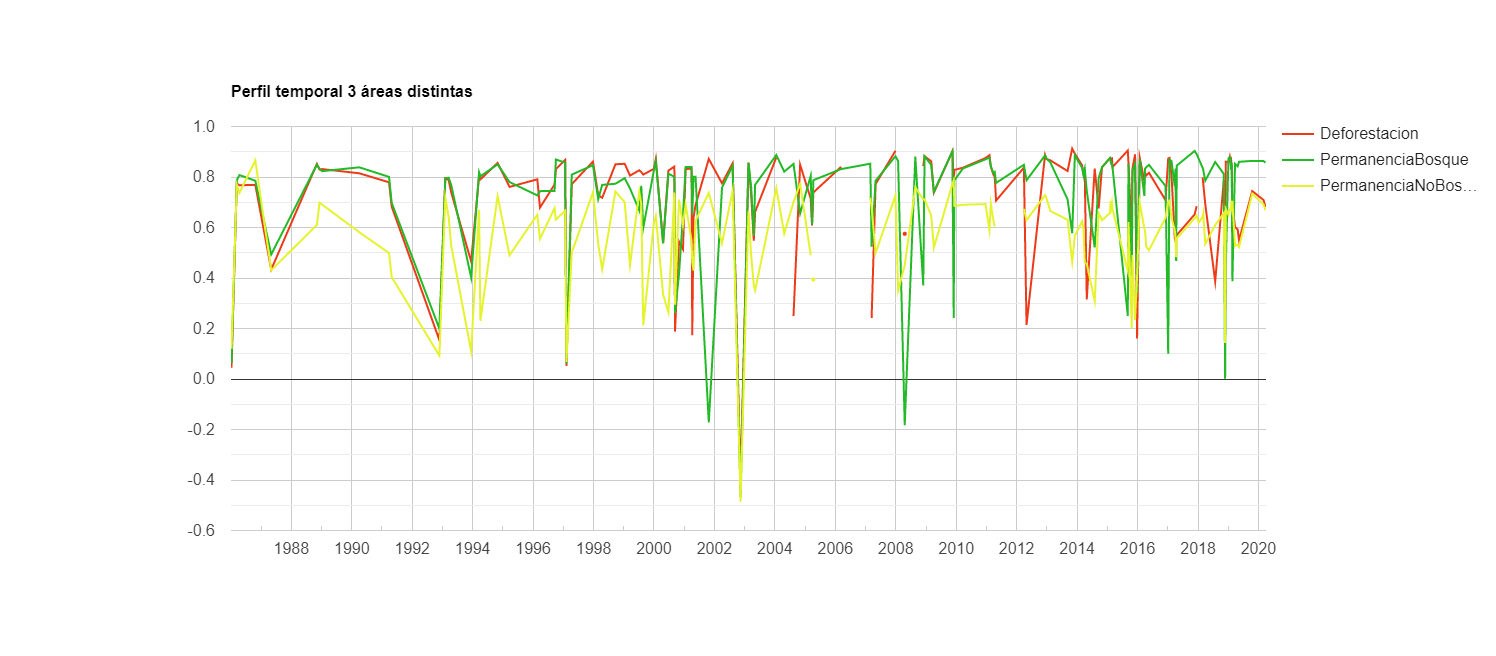
\includegraphics[width=0.95\linewidth]{Img/chartEjemplo} 

}

\caption{Ejemplo de un gráfico que muestra los perfiles temporales de un índice de vegetación (NDVI) en tres tipos de áreas: deforestación, permanencia de bosque y permanencia de no bosque.}\label{fig:f34}
\end{figure}

\begin{bluebox2}

\begin{awesomeblock}{5pt}{\faLightbulb}{darkblue}
Los nombres de las funciones para generar gráficos en GEE dan una idea del tipo de gráfica que se puede generar con dicha función y el tipo de insumos que requiere cada tipo de gráfico.

\end{awesomeblock}

\end{bluebox2}

\hypertarget{exportaciuxf3n-de-objetos-fuera-de-gee}{%
\section{Exportación de objetos fuera de GEE}\label{exportaciuxf3n-de-objetos-fuera-de-gee}}

Este grupo de funciones permite exportar algún resultado fuera de GEE para ser manejado en otro programa. Todas estas funciones se encuentran dentro de la biblioteca \boldpurple{Export}. Sin embargo, solo existen cuatro formatos válidos para exportar desde GEE: ráster (\boldpurple{ee.Image}), vector (\boldpurple{ee.FeatureCollection}), mapa y video.

\hypertarget{export.image}{%
\subsubsection*{Export.image}\label{export.image}}
\addcontentsline{toc}{subsubsection}{Export.image}

\index{Export.image}
En el caso de las imágenes (ráster, \boldpurple{ee.Image}), la función para exportarlas es \boldpurple{Export.image}. Dentro de GEE hay tres opciones para exportar los resultados de una imagen:

\begin{itemize}
\tightlist
\item
  \boldpurple{Export.image.toAsset}.
\item
  \boldpurple{Export.image.toDrive}.
\item
  \boldpurple{Export.image.toCloudStorage}.
\end{itemize}

La primera permite exportar la imagen (ráster) a la sección de \textbf{Assets}, es decir, la sección donde el usuario puede subir su información a GEE. Esta opción es útil cuando el resultado se va a utilizar en otro procedimiento de GEE. La segunda opción permite exportarla al Google Drive de la cuenta con la que se tiene acceso a GEE. Esta opción es útil para trabajar con las imágenes (rásters) en algún entorno local, como algún SIG. La última opción permite exportar la imagen al Google Cloud Storage para utilizarla en algún otro proceso a realizar en Google Cloud Platform. La opción que consideramos es más común para cualquier usuario será la de \boldpurple{Export.image.toDrive}. Al exportar información de GEE al Google Drive, se recomienda utilizar distintas carpetas para organizarla y definir su nombre en el argumento de \texttt{folder}.

\begin{bluebox2}

\begin{awesomeblock}{5pt}{\faLightbulb}{darkblue}
Solo se pueden exportar imágenes en formato \boldpurple{ee.Image}. Sin embargo, no siempre resulta obvio el formato de las imágenes, ya que algunas veces se pueden convertir a un formato de arreglo (\boldpurple{ee.Array}), tras lo cual hay que volver a convertir la información a formato de imagen (\boldpurple{ee.Image}) para poder exportarla. La aplicación permite exportar únicamente en formato GeoTiff o TFRecord (tensores), siendo la primera la opción por defecto.

\end{awesomeblock}

\end{bluebox2}

Un ejemplo de cómo exportar una imagen se presenta a continuación.

\begin{Shaded}
\begin{Highlighting}[]
\KeywordTok{Export}\OperatorTok{.}\AttributeTok{image}\OperatorTok{.}\FunctionTok{toDrive}\NormalTok{(\{}
  \CommentTok{// Definir la imagen a exportar}
  \DataTypeTok{image}\OperatorTok{:}\NormalTok{ imgDiff}\OperatorTok{,}
  \CommentTok{// Especificar el nombre con el cual se va a guardar la imagen en}
  \CommentTok{// el Google Drive}
  \DataTypeTok{description}\OperatorTok{:} \StringTok{\textquotesingle{}DiferenciaNDVI\_2016{-}2017\textquotesingle{}}\OperatorTok{,}
  \CommentTok{// Determinar el tamaño del píxel en m de la imagen a exportar}
  \DataTypeTok{scale}\OperatorTok{:} \DecValTok{30}\OperatorTok{,}
  \CommentTok{// Exportar la imagen en formato GeoTIFF}
  \DataTypeTok{fileFormat}\OperatorTok{:} \StringTok{\textquotesingle{}GeoTIFF\textquotesingle{}}\OperatorTok{,}
  \CommentTok{// Definir la carpeta del Google Drive en la que se va a exportar}
  \CommentTok{// la imagen}
  \DataTypeTok{folder}\OperatorTok{:} \StringTok{\textquotesingle{}DiferenciaNDVIL8\textquotesingle{}}
\NormalTok{\})}\OperatorTok{;} 
\end{Highlighting}
\end{Shaded}

\begin{bluebox2}

\begin{awesomeblock}{5pt}{\faLightbulb}{darkblue}
En GEE muchas operaciones utilizan el término de \texttt{scale}, sin embargo, este no se refiere a la escala de trabajo en un sentido tradicional (por ejemplo, 1:50000), sino que se refiere al tamaño de píxel expresado en metros.
En algunas ocasiones, al intentar exportar una imagen muy grande (mayor a 10 000 000 de píxeles), la consola puede mostrar un error indicando que el objeto a exportar tiene un número muy alto de píxeles. En este caso, se debe aumentar el número de píxeles máximo permitido para la exportación. Esto se logra indicando el argumento \texttt{maxPixels} dentro del diccionario que se pasa a \boldpurple{Export.image.toDrive}. Por ejemplo, \texttt{maxPixels:\ 1e10}, lo cual permite exportar una imagen con hasta 1 x 10\^{}10 píxeles.

\end{awesomeblock}

\end{bluebox2}

\hypertarget{export.table}{%
\subsubsection*{Export.table}\label{export.table}}
\addcontentsline{toc}{subsubsection}{Export.table}

\index{Export.table}
Por su parte, el formato vector (\boldpurple{ee.Feature}) permite exportar información vector y tablas sin información geográfica (o sin geometría). De nuevo, para poder exportar en el formato vector, el objeto exportado debe estar en formato de colección de vectores (\boldpurple{ee.FeatureCollection}). Al igual que en el caso de las imágenes, dentro de GEE hay tres opciones para exportar objetos de tipo vector:

\begin{itemize}
\tightlist
\item
  \boldpurple{Export.table.toAsset}.
\item
  \boldpurple{Export.table.toDrive}.
\item
  \boldpurple{Export.table.toCloudStorage}.
\end{itemize}

Para el caso de las tablas sin información geográfica asociada, se debe definir el objeto como un objeto vector sin geometría (es decir, \texttt{null}) y en la tabla de atributos anexar la información deseada. Un ejemplo del uso de esta función se presenta a continuación:

\begin{Shaded}
\begin{Highlighting}[]
\KeywordTok{Export}\OperatorTok{.}\AttributeTok{table}\OperatorTok{.}\FunctionTok{toDrive}\NormalTok{(\{}
  \CommentTok{// Definir la colección de vectores a exportar}
  \DataTypeTok{collection}\OperatorTok{:}\NormalTok{ feature}\OperatorTok{,}
  \CommentTok{// Especificar el nombre con el que se va a guardar el }
  \CommentTok{// archivo en el Google Drive}
  \DataTypeTok{description}\OperatorTok{:} \StringTok{\textquotesingle{}nombreArchivo\textquotesingle{}}\OperatorTok{,}
  \CommentTok{// Determinar la carpeta dentro de Google Drive donde}
  \CommentTok{// se va a guardar el archivo}
  \DataTypeTok{folder}\OperatorTok{:} \StringTok{\textquotesingle{}mifolder\textquotesingle{}}\OperatorTok{,}
  \CommentTok{// Exportar la información en formato csv (valores }
  \CommentTok{// delimitados por comas)}
  \DataTypeTok{fileFormat}\OperatorTok{:} \StringTok{\textquotesingle{}CSV\textquotesingle{}}
\NormalTok{\})}\OperatorTok{;}
\end{Highlighting}
\end{Shaded}

\begin{bluebox2}

\begin{awesomeblock}{5pt}{\faLightbulb}{darkblue}
GEE permite exportar información contenida en vectores solo en formatos CSV, GeoJSON, KML, KMZ, SHP o TFRecord. El primer formato es el predeterminado.

\end{awesomeblock}

\end{bluebox2}

\hypertarget{export.video}{%
\subsubsection*{Export.video}\label{export.video}}
\addcontentsline{toc}{subsubsection}{Export.video}

\index{Export.video}
Esta opción permite exportar una colección de imágenes como video, ya sea al almacenamiento de la nube de Google o al Drive.

\begin{itemize}
\tightlist
\item
  \boldpurple{Export.video.toCloudStorage}.
\item
  \boldpurple{Export.video.toDrive}.
\end{itemize}

Esta función puede resultar atractiva para observar los cambios de un área de interés a través del tiempo. A continuación se muestra cómo exportar una colección de imágenes en video:

\begin{Shaded}
\begin{Highlighting}[]
\KeywordTok{Export}\OperatorTok{.}\AttributeTok{video}\OperatorTok{.}\FunctionTok{toDrive}\NormalTok{(\{}
  \CommentTok{// Definir la colección de imágenes a exportar}
  \DataTypeTok{collection}\OperatorTok{:}\NormalTok{ coleccionImgs}\OperatorTok{,}
  \CommentTok{// Especificar el nombre con el que se va a guardar el video}
  \CommentTok{// en el Google Drive}
  \DataTypeTok{description}\OperatorTok{:} \StringTok{\textquotesingle{}videoTimelapse\textquotesingle{}}\OperatorTok{,}
  \CommentTok{// Definir la carpeta donde se va a exportar el video}
  \DataTypeTok{folder}\OperatorTok{:} \StringTok{\textquotesingle{}mifolder\textquotesingle{}}\OperatorTok{,}
  \CommentTok{// Determinar el número de cuadros por segundo}
  \DataTypeTok{framesPerSecond}\OperatorTok{:} \DecValTok{24}
\NormalTok{ \})}\OperatorTok{;}
\end{Highlighting}
\end{Shaded}

\newpage

\hypertarget{importaciuxf3n-de-informaciuxf3n-a-gee}{%
\chapter{Importación de información a GEE}\label{importaciuxf3n-de-informaciuxf3n-a-gee}}

En la sección de \textbf{Assets} se pueden importar varios tipos de archivos a GEE para utilizarlos en la API: imágenes (GeoTIFF o TFRecord), archivos vector (shapefiles), archivos separados por comas (csv), colecciones de imágenes exportadas por el mismo GEE y carpetas (\emph{folders}; \textcolor{darkblue}{Fig.} \ref{fig:f41a}, \textcolor{darkblue}{Fig.} \ref{fig:f41b}, \textcolor{darkblue}{Fig.} \ref{fig:f41c}). Para importar cualquiera de estos tipos de archivos simplemente se tiene que ingresar a la pestaña de \textbf{Assets} en el panel izquierdo y después dar clic en \textbf{New} (nuevo) e indicar el archivo que se quiere importar a GEE (\textcolor{darkblue}{Fig.} \ref{fig:f42}).

\begin{figure}[H]

{\centering \includegraphics[width=0.95\linewidth]{Img/newAssets1} 

}

\caption{Opciones disponibles para importar datos tipo raster (GeoTiff o TFRecord).}\label{fig:f41a}
\end{figure}

\begin{figure}[H]

{\centering \includegraphics[width=0.95\linewidth]{Img/newAssets2} 

}

\caption{Opciones disponibles para importar datos tipo CSV, especificar (si existe) columna de longitud y latitud (solo acepta punto decimal) y tipo de delimitador.}\label{fig:f41b}
\end{figure}

\begin{figure}[H]

{\centering \includegraphics[width=0.95\linewidth]{Img/newAssets3} 

}

\caption{Opciones disponibles para importar datos tipo Shapefile, incluir todos los archivos auxiliares.}\label{fig:f41c}
\end{figure}

\begin{figure}[H]

{\centering 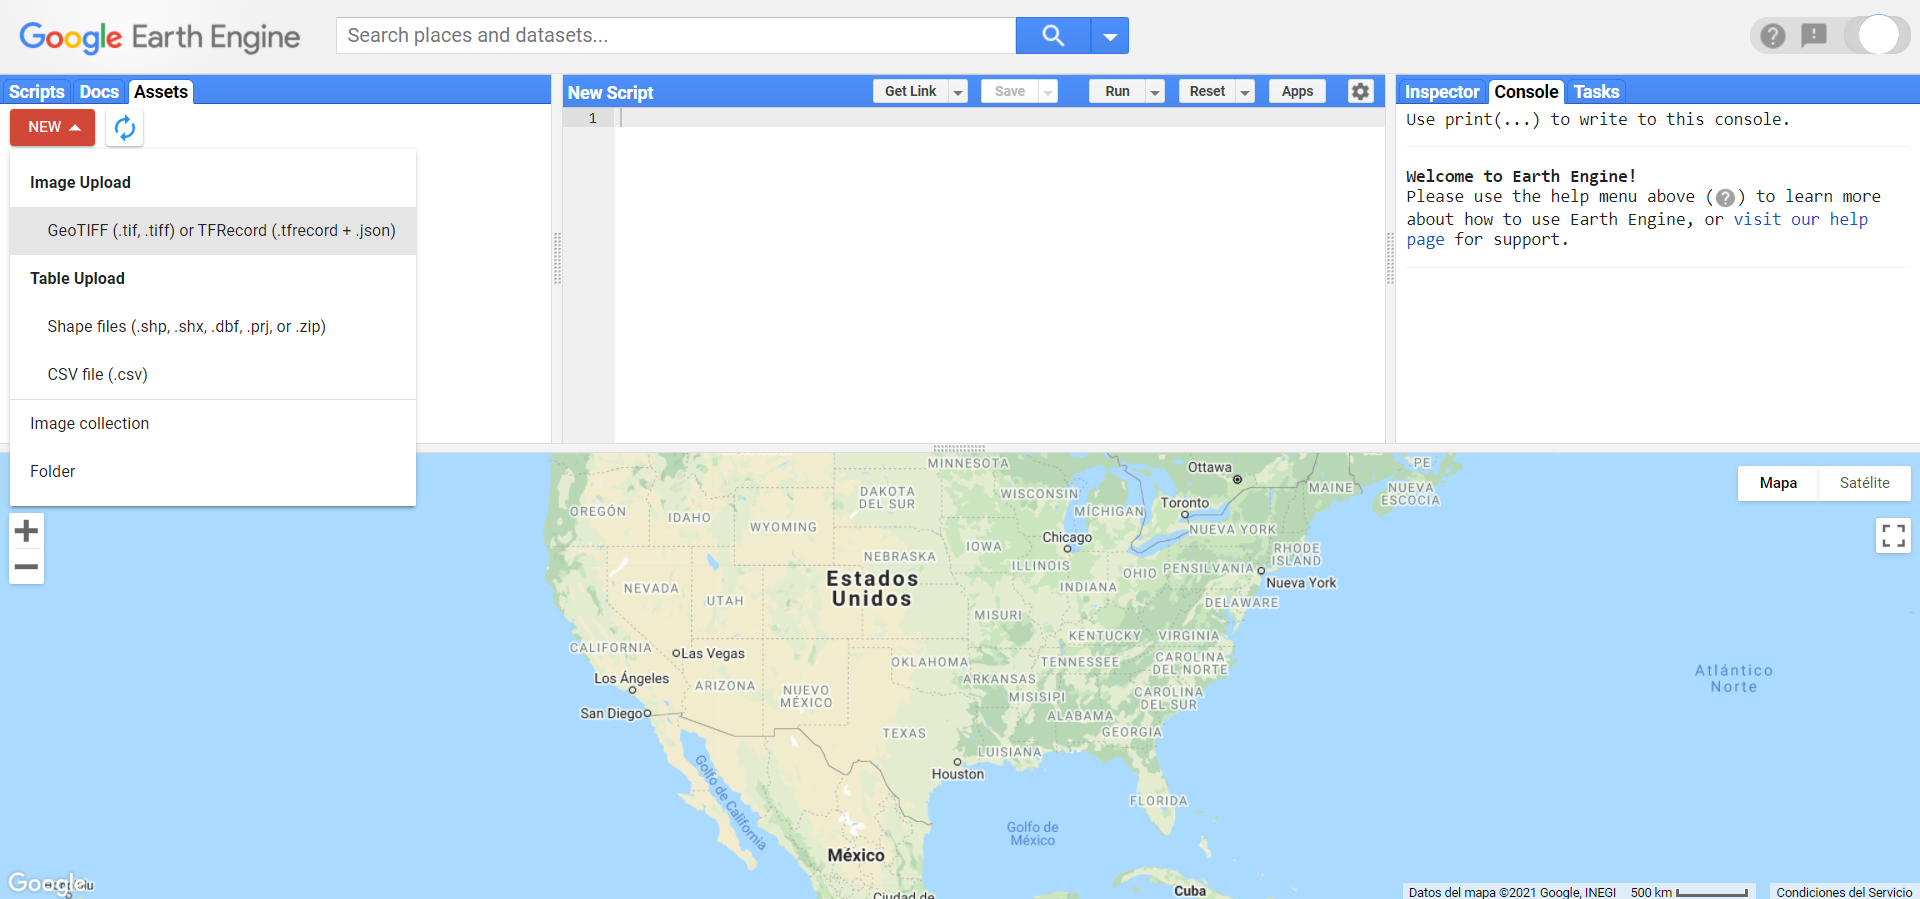
\includegraphics[width=0.95\linewidth]{Img/Asset1} 

}

\caption{Ubicación de la pestaña de importación de datos a GEE.}\label{fig:f42}
\end{figure}

Posteriormente se da clic en \textbf{Select} y se seleccionan los archivos que se quieren subir (\textcolor{darkblue}{Fig.} \ref{fig:f43}). Directamente en esta ventana se pueden agregar algunos campos a la información. Por último, se da clic en \textbf{Upload} (ubicado en la esquina inferior derecha de esta ventana) para subir los archivos a la cuenta de GEE (ocupando espacio en Google Drive). Recuerde que para archivos shapefile solo se aceptan archivos con las extensiones shp, zip, dbf, prj, shx, cpg, fix, qix, sbn o shp.xml.

\begin{figure}[H]

{\centering 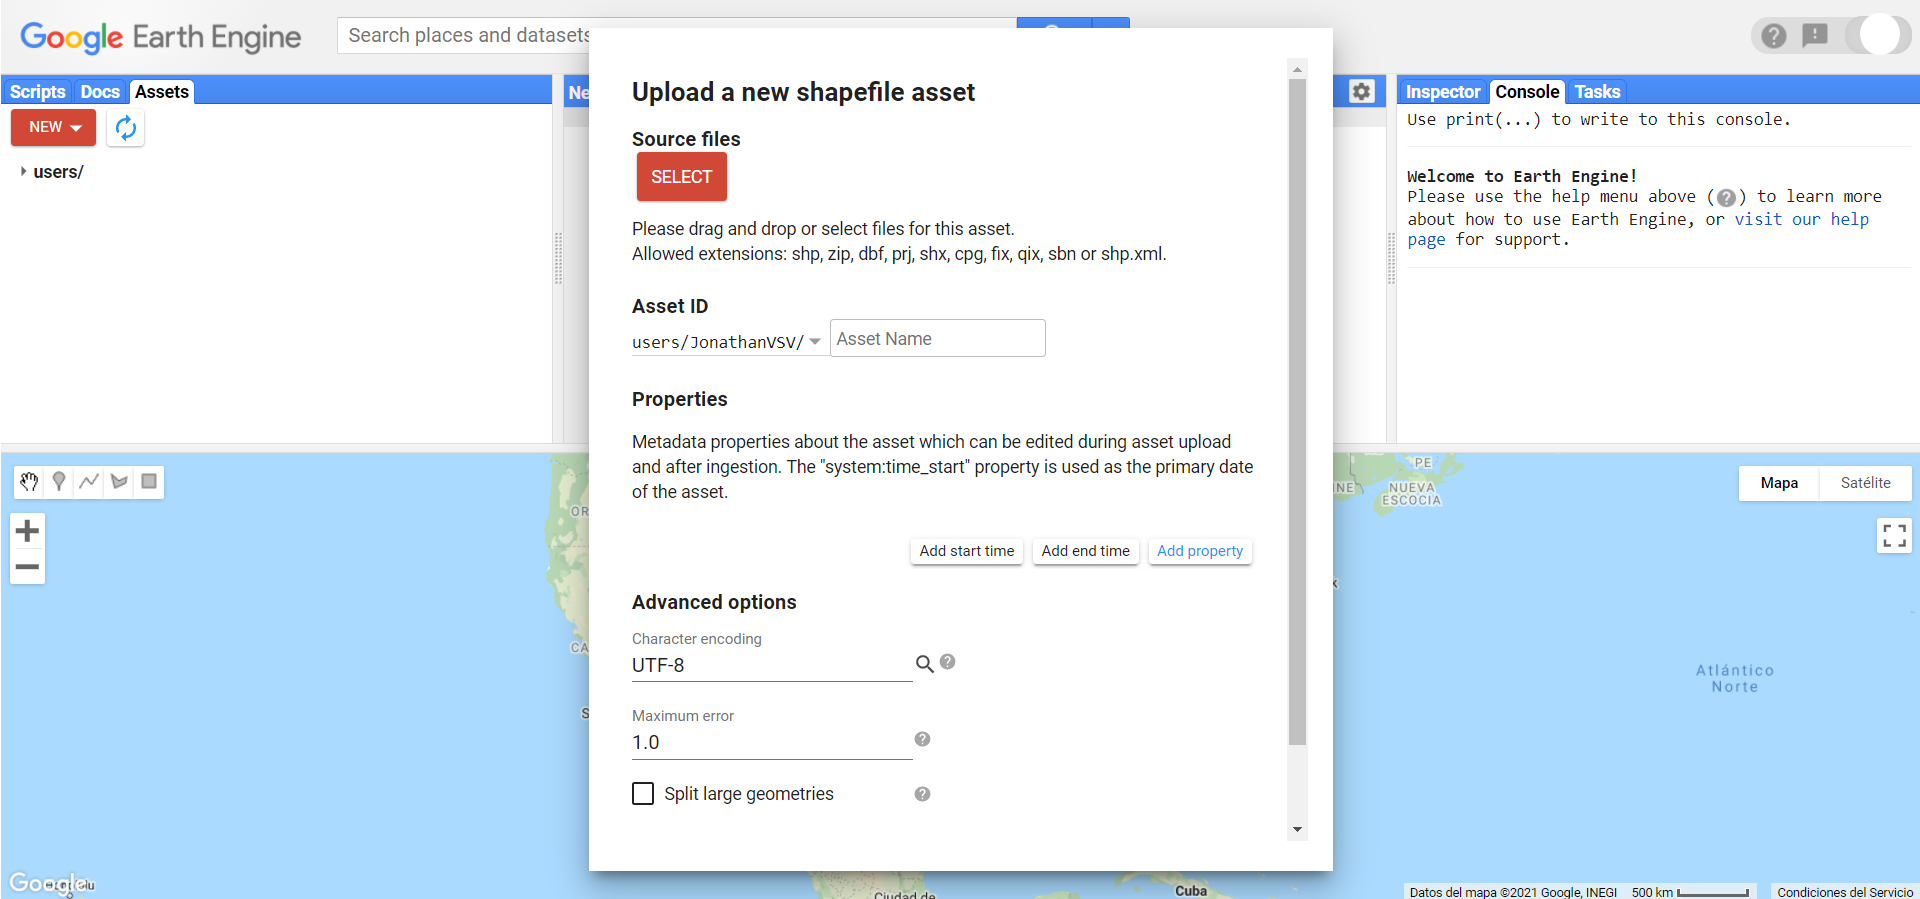
\includegraphics[width=0.95\linewidth]{Img/Asset2} 

}

\caption{Vista de la ventana de importación de datos.}\label{fig:f43}
\end{figure}

\begin{bluebox2}

\begin{awesomeblock}{5pt}{\faLightbulb}{darkblue}
Si se agrega algún otro archivo que tenga una extensión distinta a las aceptadas (shp, zip, dbf, prj, shx, cpg, fix, qix, sbn o shp.xml) la consola va a arrojar un error. En este caso hay que evitar seleccionar el archivo con la extensión que está provocando el error (por ejemplo, sbx).

\end{awesomeblock}

\end{bluebox2}

Tras haber dado clic en \textbf{Upload}, el progreso en la subida del archivo a GEE se puede consultar en la pestaña de \textbf{Tasks} (\textcolor{darkblue}{Fig.} \ref{fig:f44}). Una vez terminado, se puede tener acceso al archivo dentro de la pestaña de \textbf{Assets}. A veces no aparece el archivo recién importado, por lo cual se sugiere refrescar los elementos de esta sección presionando el botón que se encuentra a la derecha de \textbf{New}, que contiene un par de flechas formando un círculo.

\begin{figure}[H]

{\centering 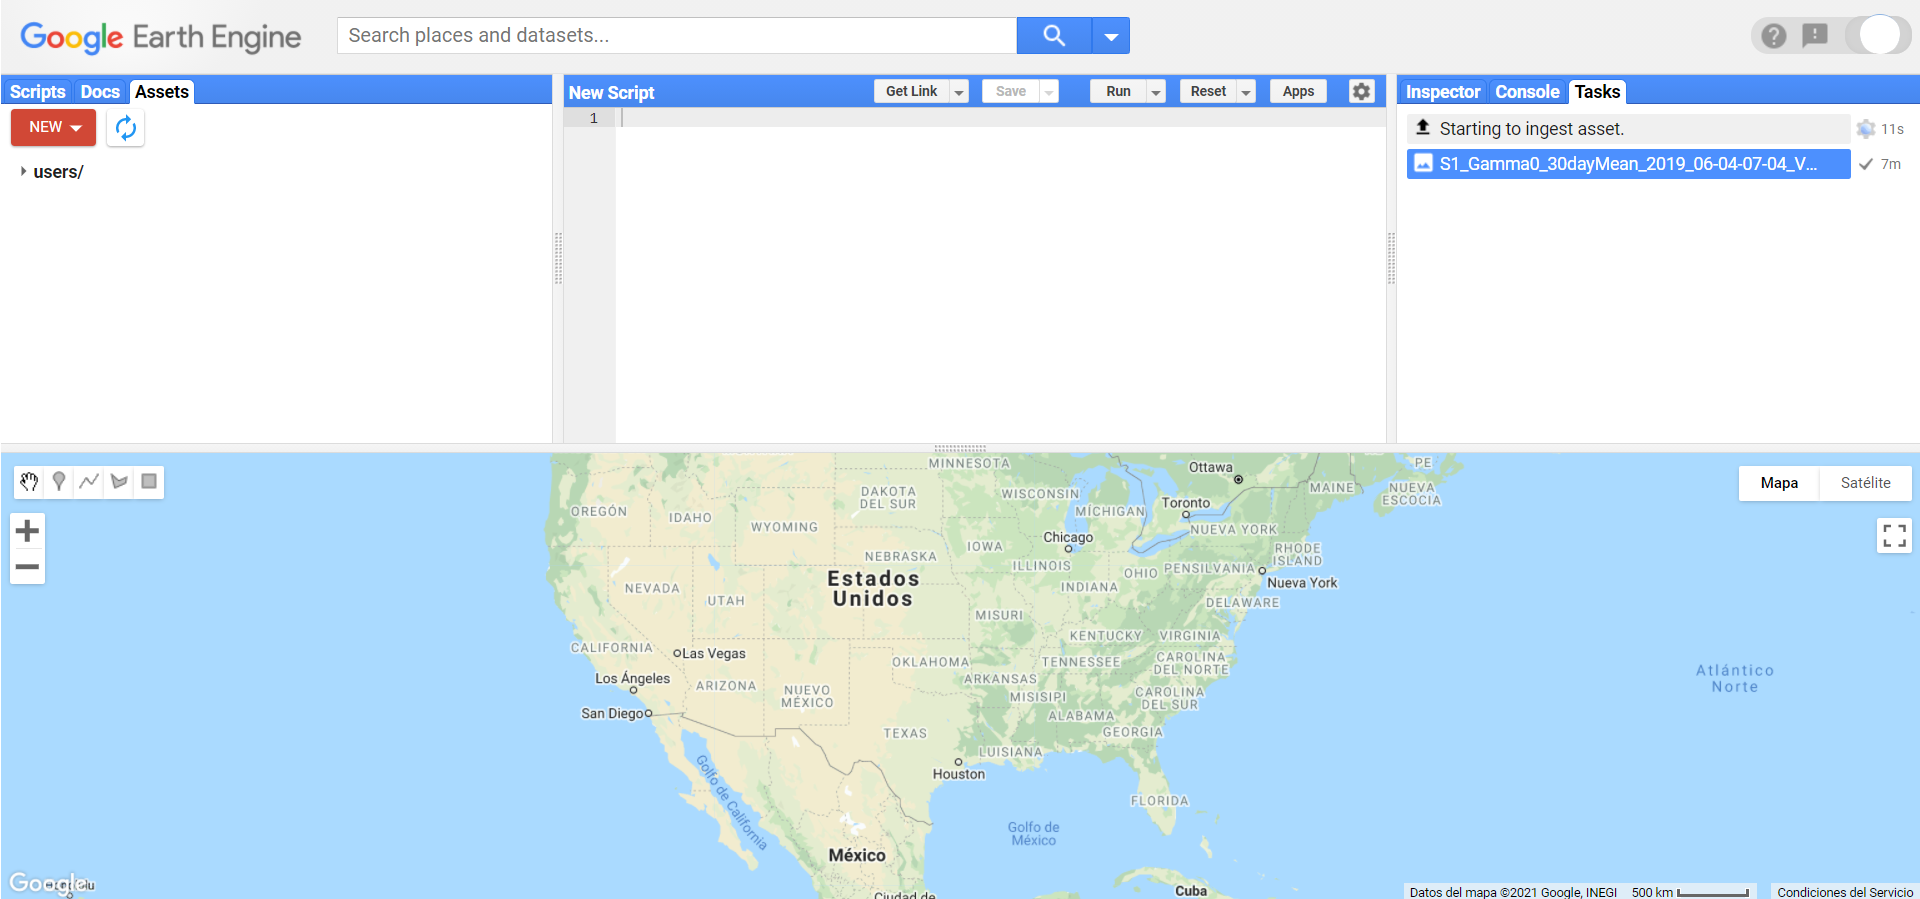
\includegraphics[width=0.95\linewidth]{Img/Asset3} 

}

\caption{Ejemplo de una importación en proceso.}\label{fig:f44}
\end{figure}

\begin{bluebox2}

\begin{awesomeblock}{5pt}{\faLightbulb}{darkblue}
Al igual que en la pestaña donde se organizan los repositorios y los códigos, en la pestaña de \textbf{Assets} se puede organizar la información en carpetas.

\end{awesomeblock}

\end{bluebox2}

Para subir un nuevo archivo hay que dar clic en el botón \textbf{New}, seleccionar el tipo de archivo y seguir las instrucciones:

\begin{enumerate}
\def\labelenumi{\arabic{enumi}.}
\tightlist
\item
  Para los archivos ráster, solo hace falta seleccionar el archivo correspondiente y dar clic en \textbf{Upload}.
\item
  Para los archivos tipo .shp es necesario subir los archivos auxiliares (dbf, prj, shx, cpg, fix, qix, sbn o shp.xml) con el mismo nombre. Para los archivos .zip es necesario que contengan los archivos auxiliares.
\item
  Para los archivos .csv es necesario que exista una columna de longitud y otra de latitud, las coordenadas deben ser decimales y estar en EPSG:4326 (WGS 84). El nombre de esas columnas se debe indicar en \textbf{Advanced options} / X column (longitud) - Y column (latitud). Además, se debe tener absoluta claridad del tipo de delimitador (ejemplo: coma, punto y coma, u otro) y este debe ser especificado en \textbf{Advanced options} / CSV delimited.
\end{enumerate}

\begin{bluebox2}

\begin{awesomeblock}{5pt}{\faLightbulb}{darkblue}
El usuario puede compartir sus archivos con otros usuarios de GEE como lector o editor. Esta opción está disponible al darle clic en el símbolo de compartir a la derecha de cada archivo (aparece una vez que se coloca el puntero sobre el nombre del archivo; \textcolor{darkblue}{Fig.} \ref{fig:f45}).

\end{awesomeblock}

\end{bluebox2}

\begin{figure}[H]

{\centering 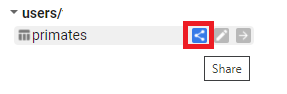
\includegraphics[width=0.5\linewidth]{Img/shareAssets} 

}

\caption{Ubicación del botón para compartir información importada en GEE.}\label{fig:f45}
\end{figure}

Por último, hay dos maneras de utilizar cualquier información importada a GEE, pero primero hay que darle clic a la información importada en la sección de \textbf{Assets}, tras lo cual aparecerá la siguiente ventana (\textcolor{darkblue}{Fig.} \ref{fig:f46}).

\begin{figure}[H]

{\centering 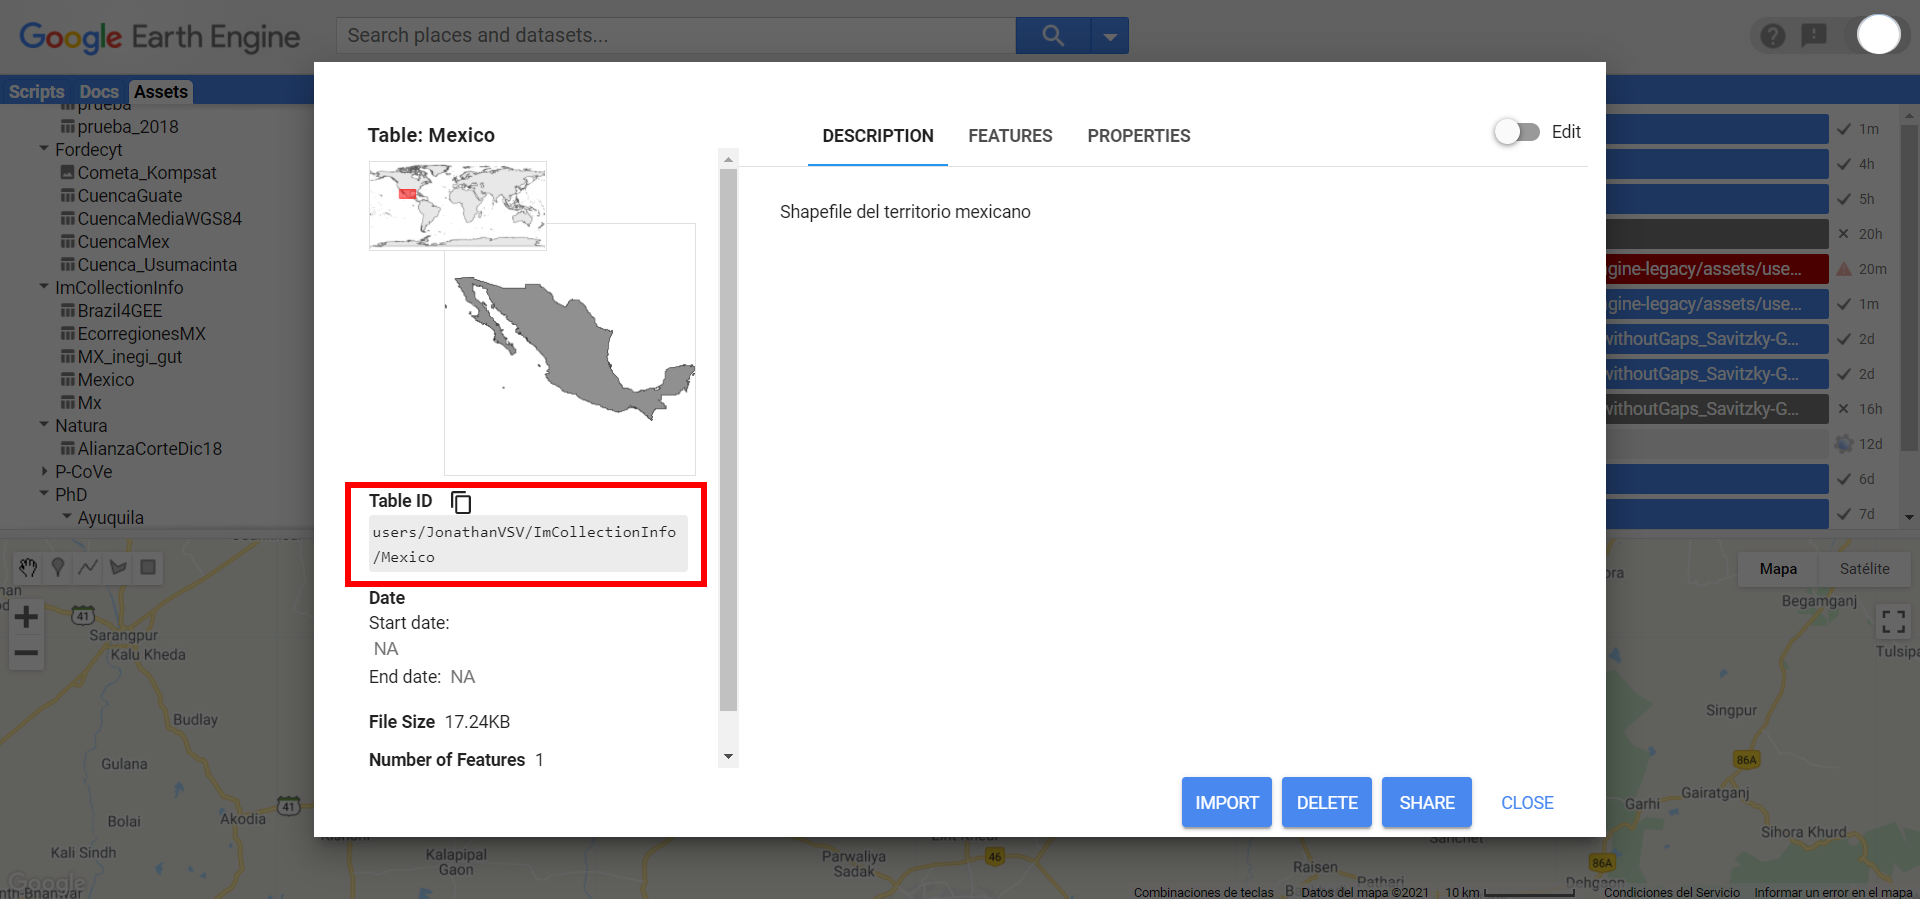
\includegraphics[width=0.95\linewidth]{Img/Asset_ruta} 

}

\caption{Ejemplo de la ventana de información importada en GEE y ubicación de la ruta de la misma.}\label{fig:f46}
\end{figure}

La primera manera consiste en copiar la ruta de la información y utilizarla en cualquier código para definir un objeto (similar a lo que se hizo en ejercicios anteriores con información hospedada en la nube de GEE; \textcolor{darkblue}{Fig.} \ref{fig:f46}).

La segunda consiste en acceder al código en el que estamos interesados en utilizar la información, buscar la información que se desea importar en la pestaña de \textbf{Assets}, darle clic, y al aparecer la misma ventana que en el ejemplo anterior, darle clic en el botón de Import (\textcolor{darkblue}{Fig.} \ref{fig:f47}). De esa manera se importa la información en el código en el que se esté trabajando y se le asigna por defecto un nombre.

\begin{figure}[H]

{\centering 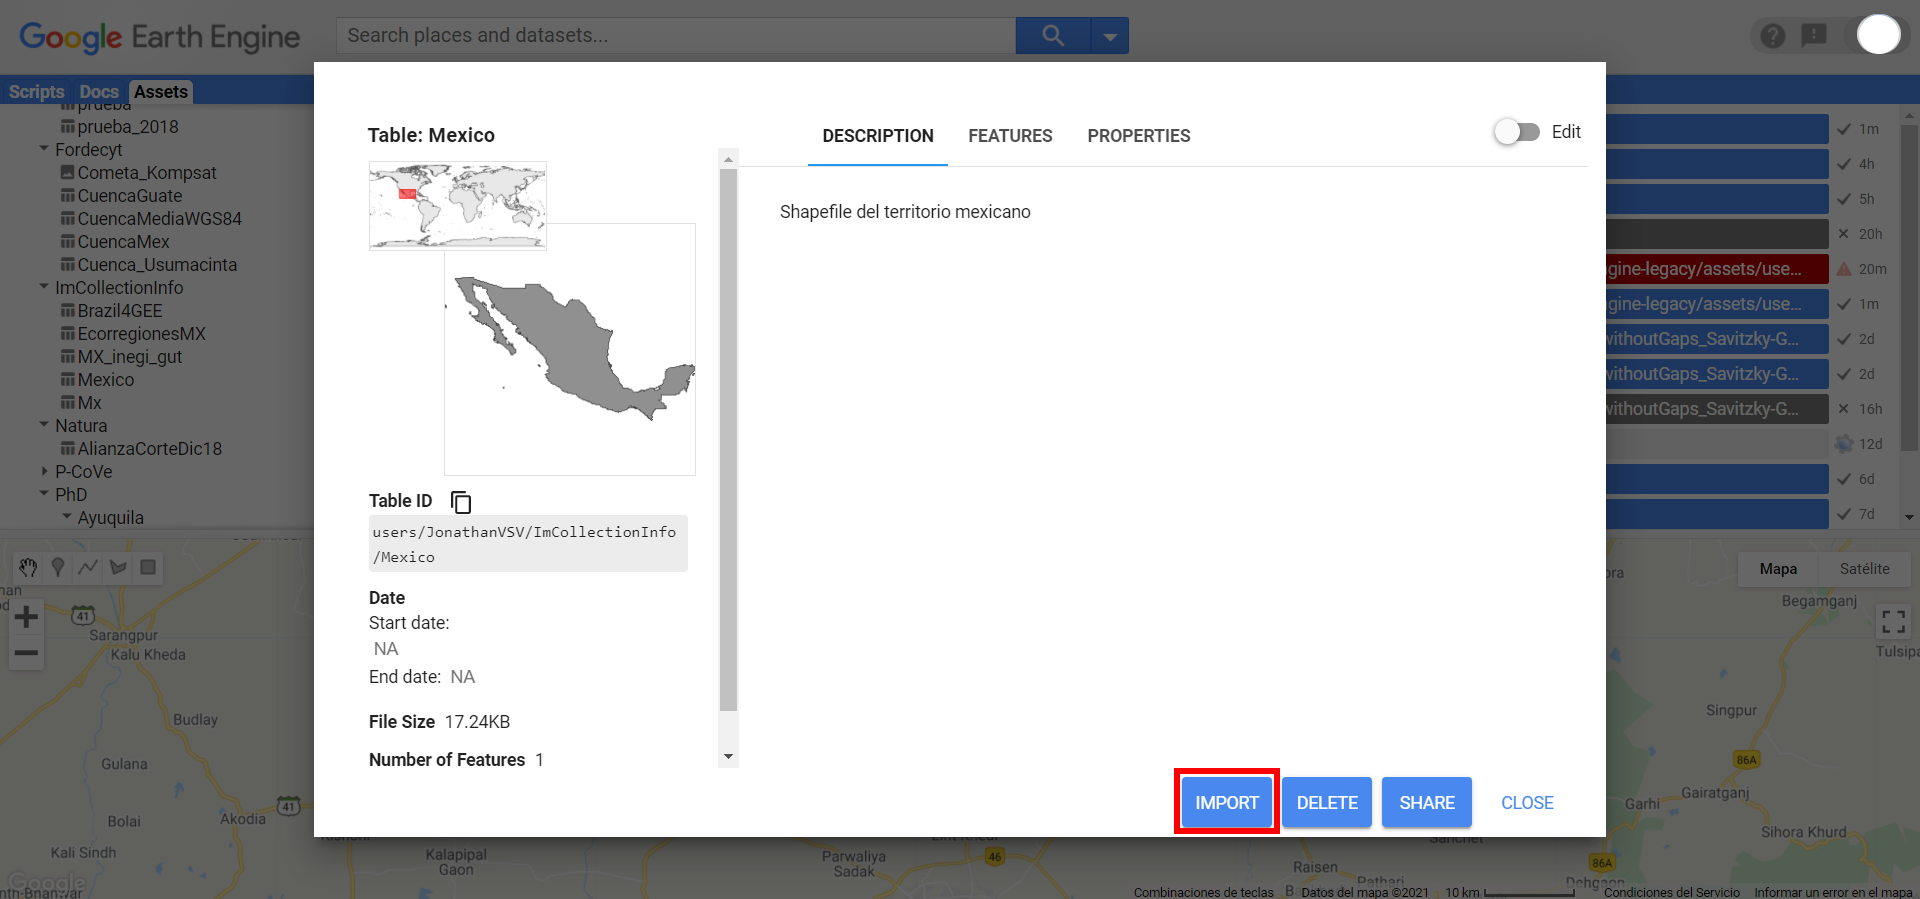
\includegraphics[width=0.95\linewidth]{Img/Asset_ruta2} 

}

\caption{Ejemplo de la ventana de información importada en GEE y ubicación del botón para importarla a un código previamente abierto.}\label{fig:f47}
\end{figure}

\newpage

\hypertarget{tipos-de-objetos}{%
\chapter{Tipos de objetos}\label{tipos-de-objetos}}

Dentro de GEE existe una amplia diversidad de tipos de objetos, por ejemplo: objetos de tipo numérico, listas, cadenas de caracteres, entre otros. Sin embargo, esta variedad de objetos se puede agrupar en dos grandes rubros: objetos del lado del cliente y objetos del servidor, según el lado donde se va a llevar a cabo el procedimiento deseado.

\hypertarget{objetos-del-cliente-y-del-servidor}{%
\section{Objetos del cliente y del servidor}\label{objetos-del-cliente-y-del-servidor}}

Existen dos lados de la programación de la API de GEE: el del servidor y el del cliente o usuario (\textcolor{darkblue}{Fig.} \ref{fig:f51}). Así, un objeto puede ser convertido entre los dos tipos. Por ejemplo, mientras que del lado del cliente una cadena de caracteres puede ser definida simplemente como: \textcolor{red}{'cadena'}, para convertirla en objeto del lado del servidor deben utilizarse las funciones del servidor, es decir: \boldpurple{ee.String}\texttt{(}\textcolor{red}{'cadena'}\texttt{)}. Adicionalmente, algunas operaciones se pueden hacer utilizando ambos tipos de sintaxis. Por ejemplo, una suma se puede realizar del lado del cliente mediante \textcolor{blue}{1} \texttt{+} \textcolor{blue}{2}, mientras que del lado del servidor se utilizará \boldpurple{ee.Number}\texttt{(}\textcolor{blue}{1}\texttt{).}\boldpurple{add}\texttt{(}\boldpurple{ee.Number}\texttt{(}\textcolor{blue}{2}\texttt{))}.

En la mayoría de los casos se va a utilizar la programación del lado del servidor, ya que es la que permite hacer todo el procesamiento en GEE. Por ejemplo, para el caso de las condiciones se sugiere utilizar en lugar de \texttt{if} y \texttt{else}, la función \boldpurple{ee.Algorithms.If}. Sin embargo, cabe aclarar que algunas funciones solo funcionan del lado del cliente. Por ejemplo, las funciones de la interfaz del usuario, utilizadas para exportar la información a algún archivo \boldpurple{ee.Export} (ya sea un ráster, un vector o una tabla), agregar una capa a la pantalla del mapa \boldpurple{Map.addLayer} o crear gráficos, así como imprimir información en la consola \boldpurple{print}. El siguiente diagrama permite visualizar el lado del usuario y del servidor en el funcionamiento de GEE.

\begin{figure}[H]

{\centering 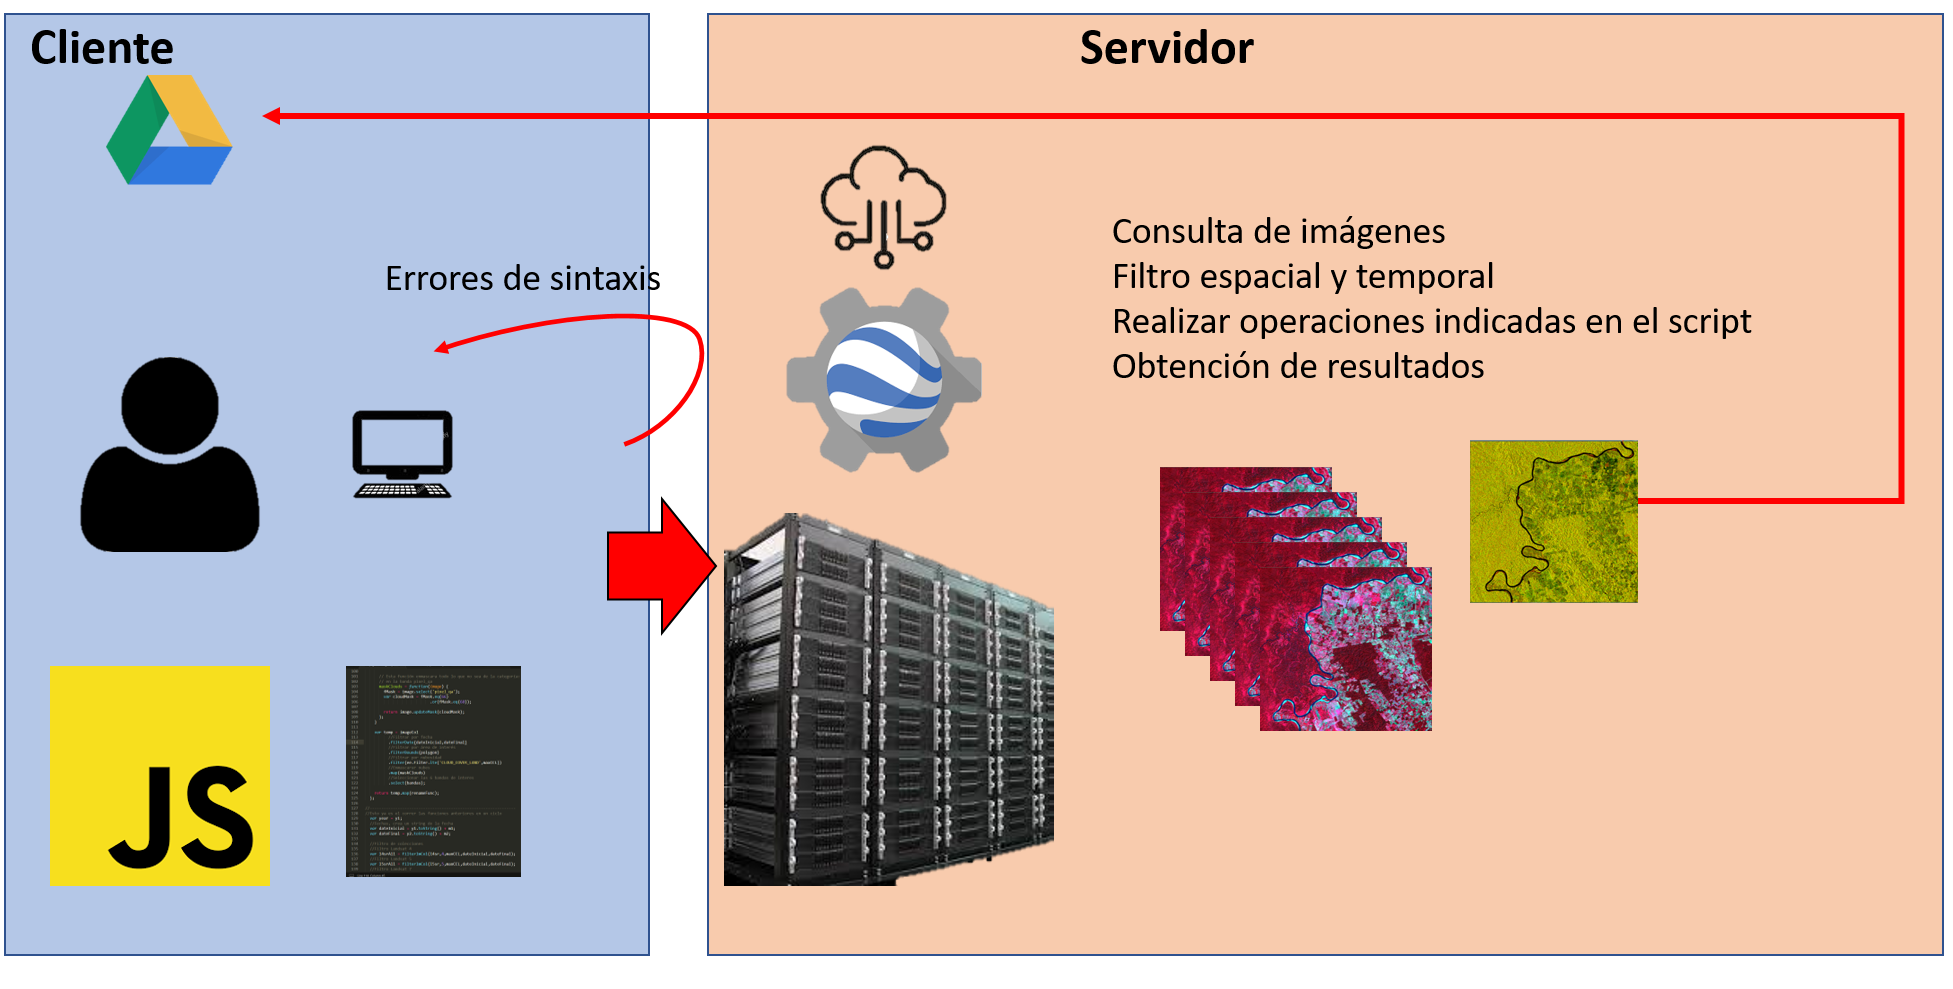
\includegraphics[width=0.95\linewidth]{Img/daigFunc} 

}

\caption{Representación de los dos lados de programación en GEE: del cliente y el servidor.}\label{fig:f51}
\end{figure}

\hypertarget{tipos-de-objetos-del-lado-del-cliente}{%
\section{Tipos de objetos del lado del cliente}\label{tipos-de-objetos-del-lado-del-cliente}}

\hypertarget{cadenas-de-texto}{%
\subsection*{Cadenas de texto}\label{cadenas-de-texto}}
\addcontentsline{toc}{subsection}{Cadenas de texto}

Se refiere a objetos de cadenas de símbolos de tipo alfanumérico. Estos se definen como cualquier cadena de caracteres (número, letras o símbolos) que se encuentren entre un par de comillas ya sean dobles \texttt{“\ ”} o sencillas \texttt{’\ ’}. Por ejemplo (\textcolor{darkblue}{Fig.} \ref{fig:f52}):

\textcolor{darkblue}{Ejercicio 0}

\begin{Shaded}
\begin{Highlighting}[]
\CommentTok{// Cadena de texto de solo letras}
\ControlFlowTok{var}\NormalTok{ cadena }\OperatorTok{=} \StringTok{\textquotesingle{}Esto es una cadena de caracteres\textquotesingle{}}\OperatorTok{;}

\CommentTok{// Cadena de texto de solo números}
\ControlFlowTok{var}\NormalTok{ telefono }\OperatorTok{=} \StringTok{\textquotesingle{}1234567890\textquotesingle{}}\OperatorTok{;}  
                     
\CommentTok{// Cadena de texto de letras, números y símbolos}
\ControlFlowTok{var}\NormalTok{ direccion }\OperatorTok{=} \StringTok{\textquotesingle{}calle cuarta casa \# 16\textquotesingle{}}\OperatorTok{;}
\end{Highlighting}
\end{Shaded}

\newpage

\textcolor{darkblue}{Ejercicio 0.1}

\begin{Shaded}
\begin{Highlighting}[]
\CommentTok{// Cadena de texto concatenada}
\ControlFlowTok{var}\NormalTok{ direccion }\OperatorTok{=}\NormalTok{ direccion }\OperatorTok{+} \StringTok{\textquotesingle{} su número telefónico es:\textquotesingle{}} \OperatorTok{+}\NormalTok{ telefono}\OperatorTok{;}
\end{Highlighting}
\end{Shaded}

\begin{bluebox2}

\begin{awesomeblock}{5pt}{\faLightbulb}{darkblue}
Los números en una cadena de texto no serán interpretados como valores numéricos sino como texto.

\end{awesomeblock}

\end{bluebox2}

\begin{figure}[H]

{\centering 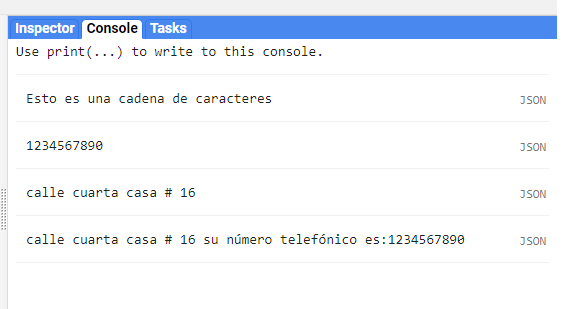
\includegraphics[width=0.8\linewidth]{Img/ej0} 

}

\caption{Salida de la consola de objetos de tipo cadena de caracteres.}\label{fig:f52}
\end{figure}

\hypertarget{nuxfameros}{%
\subsection*{Números}\label{nuxfameros}}
\addcontentsline{toc}{subsection}{Números}

Se refiere a objetos numéricos que indican un valor. Para números decimales se utiliza el punto decimal y no la coma decimal. Por ejemplo (\textcolor{darkblue}{Fig.} \ref{fig:f53}):

\textcolor{darkblue}{Ejercicio 1}

\begin{Shaded}
\begin{Highlighting}[]
\CommentTok{// Número entero}
\ControlFlowTok{var}\NormalTok{ numero }\OperatorTok{=} \DecValTok{1}\OperatorTok{;} 
 
\CommentTok{// Número decimal con punto decimal  }
\ControlFlowTok{var}\NormalTok{ numero2 }\OperatorTok{=} \FloatTok{2.5}\OperatorTok{;}  
\end{Highlighting}
\end{Shaded}

\begin{figure}[H]

{\centering 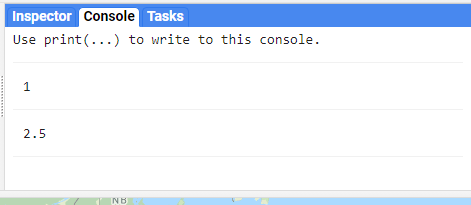
\includegraphics[width=0.95\linewidth]{Img/ej1} 

}

\caption{Salida de la consola de objetos de tipo número.}\label{fig:f53}
\end{figure}

\begin{bluebox2}

\begin{awesomeblock}{5pt}{\faLightbulb}{darkblue}
Para los objetos numéricos no se usan las comillas.

\end{awesomeblock}

\end{bluebox2}

\hypertarget{listas}{%
\subsection*{Listas}\label{listas}}
\addcontentsline{toc}{subsection}{Listas}

Las listas se refieren a objetos que contienen varias entradas, las cuales pueden ser numéricas (números), cadenas de texto (texto) o incluso otras listas. Las listas se definen mediante el uso de corchetes \texttt{{[}{]}} y cada entrada es separada mediante una coma \texttt{,} . Por ejemplo (\textcolor{darkblue}{Fig.} \ref{fig:f54}):

\textcolor{darkblue}{Ejercicio 2}

\begin{Shaded}
\begin{Highlighting}[]
\CommentTok{// Lista numérica}
\ControlFlowTok{var}\NormalTok{ lista }\OperatorTok{=}\NormalTok{ [}\DecValTok{1}\OperatorTok{,} \DecValTok{2}\OperatorTok{,} \DecValTok{3}\OperatorTok{,} \DecValTok{4}\OperatorTok{,} \DecValTok{5}\OperatorTok{,} \DecValTok{6}\OperatorTok{,} \DecValTok{7}\OperatorTok{,} \DecValTok{8}\NormalTok{]}\OperatorTok{;}   
  
\CommentTok{// Lista de texto            }
\ControlFlowTok{var}\NormalTok{ listaA }\OperatorTok{=}\NormalTok{ [}\StringTok{\textquotesingle{}primero\textquotesingle{}}\OperatorTok{,} \StringTok{\textquotesingle{}segundo\textquotesingle{}}\OperatorTok{,} \StringTok{\textquotesingle{}tercero\textquotesingle{}}\NormalTok{]}\OperatorTok{;} 
   
\CommentTok{// Lista de texto y números  }
\ControlFlowTok{var}\NormalTok{ listaB }\OperatorTok{=}\NormalTok{ [}\StringTok{\textquotesingle{}primero\textquotesingle{}}\OperatorTok{,} \StringTok{\textquotesingle{}segundo\textquotesingle{}}\OperatorTok{,} \StringTok{\textquotesingle{}tercero\textquotesingle{}}\OperatorTok{,} \DecValTok{4}\NormalTok{]}\OperatorTok{;} 

\CommentTok{// Lista de listas  }
\ControlFlowTok{var}\NormalTok{ listaC }\OperatorTok{=}\NormalTok{ [lista}\OperatorTok{,}\NormalTok{ listaA}\OperatorTok{,}\NormalTok{ listaB]}\OperatorTok{;} 
\end{Highlighting}
\end{Shaded}

Todas las listas automáticamente asignan, en orden, un número a cada elemento dentro de ellas, siempre empezando desde 0. Se puede consultar un solo elemento dentro de una lista, indicando el número de su posición dentro de ella.
\newpage
\textcolor{darkblue}{Ejercicio 2.1}

\begin{Shaded}
\begin{Highlighting}[]
\CommentTok{// Primer objeto de la lista llamada \textquotesingle{}lista\textquotesingle{}}
\FunctionTok{print}\NormalTok{(lista[}\DecValTok{0}\NormalTok{])}\OperatorTok{;} 

\CommentTok{// Segundo objeto de la lista llamada \textquotesingle{}listaA\textquotesingle{}}
\FunctionTok{print}\NormalTok{(listaA[}\DecValTok{1}\NormalTok{])}\OperatorTok{;}

\CommentTok{// Tercer objeto de la lista llamada \textquotesingle{}listaB\textquotesingle{}}
\FunctionTok{print}\NormalTok{(listaB[}\DecValTok{2}\NormalTok{])}\OperatorTok{;}

\CommentTok{// Lista completa con todos sus elementos}
\FunctionTok{print}\NormalTok{(listaC)}\OperatorTok{;}    
\end{Highlighting}
\end{Shaded}

\begin{figure}[H]

{\centering 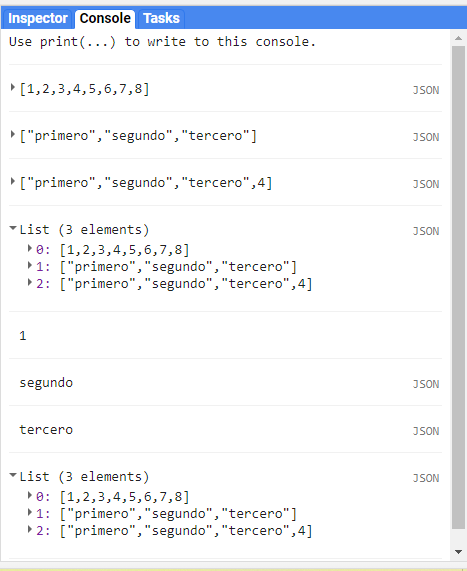
\includegraphics[width=0.6\linewidth]{Img/ej2} 

}

\caption{Salida de la consola de varios objetos de tipo lista.}\label{fig:f54}
\end{figure}

\hypertarget{diccionarios}{%
\subsection*{Diccionarios}\label{diccionarios}}
\addcontentsline{toc}{subsection}{Diccionarios}

Los diccionarios son objetos que contienen claves (entradas) y valores asociados a estas claves (definiciones). Los diccionarios se crean mediante el uso de llaves \texttt{\{\}} donde se indica cada clave seguida de dos puntos \texttt{:} y su definición, ya sea un valor, cadena de caracteres o lista asociada a esa clave. Para ingresar varias entradas, estas deben ir separadas por una coma.

Las claves o entradas siempre serán leídas como cadenas de texto. Se recomienda que no haya espacios dentro de ellas, en su lugar se aconseja usar guion bajo (\texttt{\_}) o la notación de \emph{lowerCamelCase}. Al hacer \boldpurple{print} se ordenarán alfabéticamente las claves (\textcolor{darkblue}{Fig.} \ref{fig:f55}).

\textcolor{darkblue}{Ejercicio 3}

\begin{Shaded}
\begin{Highlighting}[]
\CommentTok{// Se declara un nuevo diccionario.}
\CommentTok{// La primera entrada es el texto \textquotesingle{}clave1\textquotesingle{} que está definido con el valor}
\CommentTok{// de 1 (tipo número) la segunda entrada es el texto \textquotesingle{}clave2\textquotesingle{}, y su }
\CommentTok{// definición es la letra \textquotesingle{}A\textquotesingle{} (tipo cadena de texto)}
\ControlFlowTok{var}\NormalTok{ dicc }\OperatorTok{=}\NormalTok{ \{   }
  \DataTypeTok{clave1}\OperatorTok{:} \DecValTok{1}\OperatorTok{,}      
  \DataTypeTok{clave2}\OperatorTok{:} \StringTok{\textquotesingle{}A\textquotesingle{}}  
\NormalTok{\}}\OperatorTok{;}            
      
\end{Highlighting}
\end{Shaded}

Hay dos formas de consultar los valores dentro de un diccionario (Fig. 5.5):

\begin{itemize}
\tightlist
\item
  Llamar directamente el nombre de la clave deseada dentro de comillas en un par de corchetes \texttt{{[}\textquotesingle{}\textquotesingle{}{]}}.
\item
  Utilizar la notación de \texttt{.} (punto) seguida del nombre de la clave.
\end{itemize}

Por ejemplo:

\textcolor{darkblue}{Ejercicio 3.1}

\begin{Shaded}
\begin{Highlighting}[]
\CommentTok{// Notación de lista, se mostrará en la consola la definición de }
\CommentTok{// \textquotesingle{}clave1\textquotesingle{}, es decir el valor 1 }
\FunctionTok{print}\NormalTok{(dicc[}\StringTok{\textquotesingle{}clave1\textquotesingle{}}\NormalTok{])}\OperatorTok{;} 

\CommentTok{// Notación de lista, se mostrará en la consola la definición de }
\CommentTok{// \textquotesingle{}clave2\textquotesingle{}, es decir la letra \textquotesingle{}A\textquotesingle{}}
\FunctionTok{print}\NormalTok{(dicc[}\StringTok{\textquotesingle{}clave2\textquotesingle{}}\NormalTok{])}\OperatorTok{;}  

\CommentTok{// Notación con punto, se mostrará en la consola la definición de }
\CommentTok{// \textquotesingle{}clave1\textquotesingle{}, es decir el valor 1 }
\FunctionTok{print}\NormalTok{(dicc}\OperatorTok{.}\AttributeTok{clave1}\NormalTok{)}\OperatorTok{;}  

\CommentTok{// Notación con punto, se mostrará en la consola la definición de }
\CommentTok{// \textquotesingle{}clave2\textquotesingle{}, es decir la letra \textquotesingle{}A\textquotesingle{}}
\FunctionTok{print}\NormalTok{(dicc}\OperatorTok{.}\AttributeTok{clave2}\NormalTok{)}\OperatorTok{;}  
\end{Highlighting}
\end{Shaded}

\begin{figure}[H]

{\centering 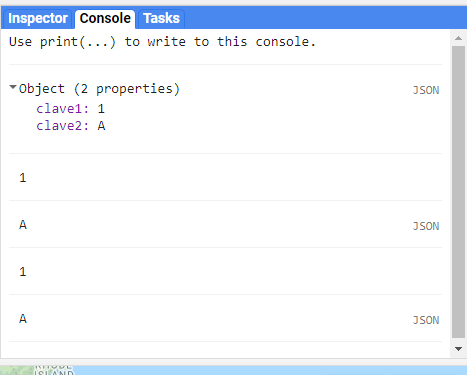
\includegraphics[width=0.6\linewidth]{Img/ej3} 

}

\caption{Salida de la consola de varios objetos de tipo diccionario.}\label{fig:f55}
\end{figure}

\begin{bluebox2}

\begin{awesomeblock}{5pt}{\faLightbulb}{darkblue}
Para los diccionarios se recomienda utilizar la notación de \texttt{.} (punto) seguida del nombre de la clave, ya que es la recomendada por GEE.

\end{awesomeblock}

\end{bluebox2}

\hypertarget{funciones}{%
\subsection*{Funciones}\label{funciones}}
\addcontentsline{toc}{subsection}{Funciones}

\index{function}
Se refiere a objetos que contienen algún proceso que se realizará a alguna variable. Siempre comienzan con la palabra \texttt{function} (función) seguida por el objeto al que se le aplicará la función. Este objeto debe escribirse entre paréntesis y entre llaves se coloca el procedimiento que va a realizar la función. Por último, debe regresar un objeto mediante la función \texttt{return}. Por ejemplo:

\begin{Shaded}
\begin{Highlighting}[]
\CommentTok{// MaskIm es una nueva función, y su argumento de entrada es objeto}
\ControlFlowTok{var}\NormalTok{ maskIm }\OperatorTok{=} \ControlFlowTok{function}\NormalTok{(objeto)\{ }
  \CommentTok{// Se define qué objeto es una imagen ráster y se guarda en la }
  \CommentTok{// variable image}
  \ControlFlowTok{var}\NormalTok{ image }\OperatorTok{=} \KeywordTok{ee}\OperatorTok{.}\FunctionTok{Image}\NormalTok{(objeto)}\OperatorTok{;}
   
  \CommentTok{// Se selecciona solamente la banda de nombre \textquotesingle{}pixel\_qa\textquotesingle{} de la imagen}
  \CommentTok{// image}
  \ControlFlowTok{var}\NormalTok{ qaImage }\OperatorTok{=}\NormalTok{ image}\OperatorTok{.}\FunctionTok{select}\NormalTok{(}\StringTok{\textquotesingle{}pixel\_qa\textquotesingle{}}\NormalTok{)}\OperatorTok{;}
       
  \CommentTok{// Se crea una nueva imagen binaria donde será 1 los píxeles con valor }
  \CommentTok{// igual a 322, y 0 los demás}
  \ControlFlowTok{var}\NormalTok{ clearData }\OperatorTok{=}\NormalTok{ qaImage}\OperatorTok{.}\FunctionTok{eq}\NormalTok{(}\DecValTok{322}\NormalTok{)}\OperatorTok{;}      
      
  \CommentTok{// Se crea una máscara con la imagen binaria, y se entrega la imagen }
  \CommentTok{// original enmascarada}
  \ControlFlowTok{return}\NormalTok{ image}\OperatorTok{.}\FunctionTok{updateMask}\NormalTok{(clearData)}\OperatorTok{;}      
\NormalTok{ \}}\OperatorTok{;}
\end{Highlighting}
\end{Shaded}

Aunque las funciones son propiamente objetos del lado del cliente, deben contener únicamente métodos del lado del servidor para que funcionen apropiadamente al trabajar en GEE. Esto permite que GEE interprete cualquier serie de procesos de manera adecuada en sus servidores. Esto quedará más claro después de repasar la siguiente sección.

\begin{bluebox2}

\begin{awesomeblock}{5pt}{\faLightbulb}{darkblue}
Las funciones que se ejecuten sobre una colección de imágenes o vectores solo funcionan si regresan un objeto de tipo \boldpurple{ee.Feature}, \boldpurple{ee.FeatureCollection}, \boldpurple{ee.Image} o \boldpurple{ee.ImageCollection}, por lo cual, a veces, se deben realizar ciertas conversiones para evitar un error.

\end{awesomeblock}

\end{bluebox2}

\hypertarget{tipo-de-objetos-del-lado-del-servidor}{%
\section{Tipo de objetos del lado del servidor}\label{tipo-de-objetos-del-lado-del-servidor}}

Los objetos del lado del servidor, además de permitir llevar a cabo procesos en los servidores de GEE, tienen asociados una serie de métodos particulares por tipo de objeto. Esto quiere decir que al convertir un objeto del lado del cliente al del servidor, automáticamente se abre la posibilidad de utilizar los métodos precargados en GEE para ese tipo de objeto. Toda la información que se encuentra disponible en GEE corresponderá a objetos del servidor, entre los que destacan los objetos de tipo imagen (ráster), vector, colecciones de imágenes y colecciones de vectores.

\begin{bluebox2}

\begin{awesomeblock}{5pt}{\faLightbulb}{darkblue}
Para saber cuáles objetos son del servidor, resulta útil recordar que todos ellos cuentan con el prefijo \boldpurple{ee}\texttt{.} (del servidor de Earth Engine) seguido del nombre del tipo de objeto con inicial mayúscula.

\end{awesomeblock}

\end{bluebox2}

Los objetos del lado del servidor se pueden conceptualizar como contenedores que le indican al servidor qué tipo de objeto es el que se está enviando. Además, cuando se trabaja del lado del servidor, los objetos necesariamente son enviados al servidor para ser evaluados. A continuación se describen los tipos de objetos que más se usan (\textcolor{darkblue}{Fig.} \ref{fig:f56}).

\begin{bluebox2}

\begin{awesomeblock}{5pt}{\faLightbulb}{darkblue}
En algunos casos, los objetos que se obtienen a partir de ciertos métodos retornan un objeto de tipo indefinido (tipo objeto, \boldpurple{ee.Object}) como por ejemplo, al usar, en casos particulares, los métodos \texttt{.}\boldpurple{first} o \texttt{.}\boldpurple{get}, por lo cual se recomienda meter este objeto indefinido en un contenedor que indique el tipo de objeto del servidor. De no hacerlo, GEE mostrará un error \texttt{...is\ not\ a\ function}.

\end{awesomeblock}

\end{bluebox2}

\begin{bluebox2}

\begin{awesomeblock}{5pt}{\faLightbulb}{darkblue}
Todos los métodos disponibles en GEE clasificados por tipo de objeto del servidor se pueden consultar en la sección de \textbf{Client libraries} en el siguiente enlace: \url{https://developers.google.com/earth-engine/apidocs}. En \textbf{Client libraries} se indican cuáles argumentos acepta cada método o función, así como el tipo de objeto de la salida.

\end{awesomeblock}

\end{bluebox2}



\begin{figure}[H]

{\centering 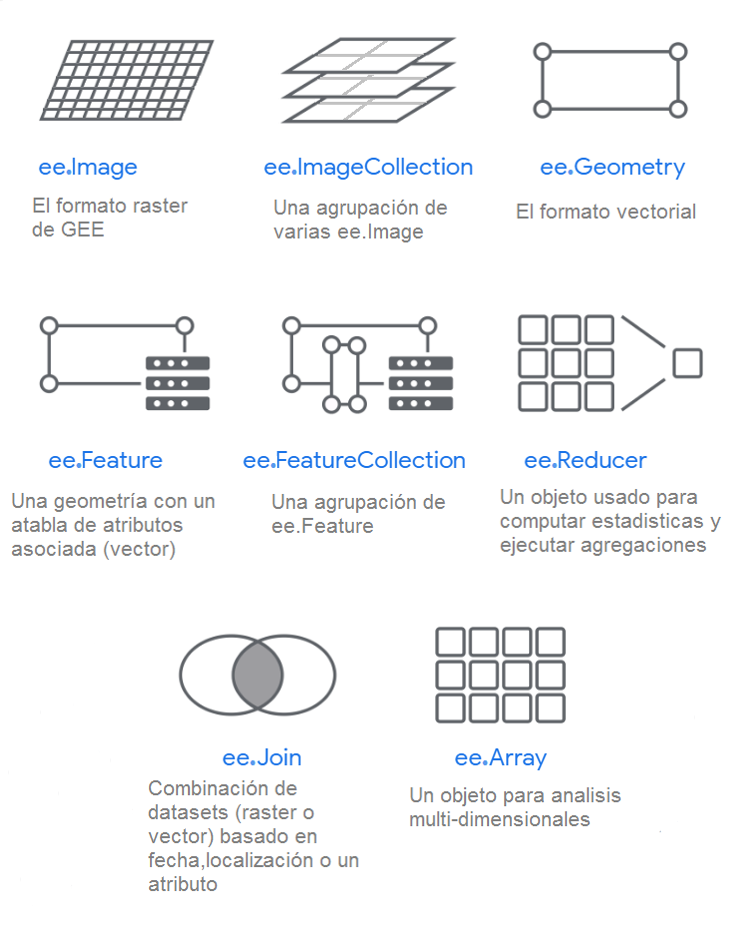
\includegraphics[width=0.95\linewidth]{Img/objetosServ2} 

}

\caption{Diagrama con algunos de los objetos del lado del servidor más utilizados en GEE. Tomado y modificado de \url{https://developers.google.com/earth-engine/guides/objects_methods_overview}.}\label{fig:f56}
\end{figure}

\hypertarget{ee.string}{%
\subsection*{ee.String}\label{ee.string}}
\addcontentsline{toc}{subsection}{ee.String}

\index{ee.String}
Este tipo de objeto es equivalente a la cadena de texto pero del lado del servidor, ya que permite enviar un objeto como cadena de caracteres al servidor. Por ejemplo (\textcolor{darkblue}{Fig.} \ref{fig:f57}):

\textcolor{darkblue}{Ejercicio 4}

\begin{Shaded}
\begin{Highlighting}[]
\CommentTok{// Esta es una cadena de texto del lado del cliente}
\ControlFlowTok{var}\NormalTok{ cadena2 }\OperatorTok{=} \StringTok{\textquotesingle{}Esto es una cadena de caracteres\textquotesingle{}}\OperatorTok{;}
\CommentTok{// En este paso se convierte el texto del lado del cliente a un ee.String}
\CommentTok{// del lado del servidor}
\ControlFlowTok{var}\NormalTok{ cadenaServ }\OperatorTok{=} \KeywordTok{ee}\OperatorTok{.}\FunctionTok{String}\NormalTok{(cadena2)}\OperatorTok{;}                         
\end{Highlighting}
\end{Shaded}

\begin{figure}[H]

{\centering 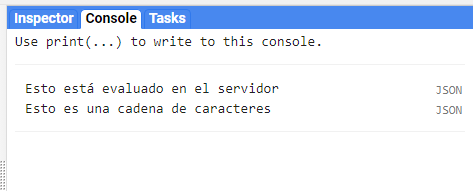
\includegraphics[width=0.95\linewidth]{Img/ej4} 

}

\caption{Salida de la consola de un objeto de tipo cadena de caracteres del lado del servidor.}\label{fig:f57}
\end{figure}

\hypertarget{ee.number}{%
\subsection*{ee.Number}\label{ee.number}}
\addcontentsline{toc}{subsection}{ee.Number}

\index{ee.Number}
Permite enviar un número como objeto al servidor. Por ejemplo (\textcolor{darkblue}{Fig.} \ref{fig:f58}):

\textcolor{darkblue}{Ejercicio 5}

\begin{Shaded}
\begin{Highlighting}[]
\CommentTok{// Se define un número como ee.Number del servidor}
\ControlFlowTok{var}\NormalTok{ numServ }\OperatorTok{=} \KeywordTok{ee}\OperatorTok{.}\FunctionTok{Number}\NormalTok{(}\DecValTok{1900}\NormalTok{)}\OperatorTok{;}                              
\end{Highlighting}
\end{Shaded}

\begin{figure}[H]

{\centering 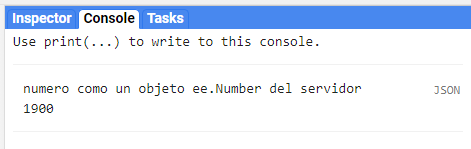
\includegraphics[width=0.95\linewidth]{Img/ej5} 

}

\caption{Salida de la consola de un objeto de tipo número del lado del servidor.}\label{fig:f58}
\end{figure}

\hypertarget{ee.list}{%
\subsection*{ee.List}\label{ee.list}}
\addcontentsline{toc}{subsection}{ee.List}

\index{ee.List}
Este tipo de objetos corresponden a listas del lado del servidor. Por ejemplo (\textcolor{darkblue}{Fig.} \ref{fig:f59}):

\textcolor{darkblue}{Ejercicio 6}

\begin{Shaded}
\begin{Highlighting}[]
\CommentTok{// Se construye una nueva lista con diferentes tipos de objetos del lado }
\CommentTok{// del usuario y servidor}
\ControlFlowTok{var}\NormalTok{ lista }\OperatorTok{=}\NormalTok{ [}\StringTok{\textquotesingle{}hola\textquotesingle{}}\OperatorTok{,}\StringTok{\textquotesingle{}12\textquotesingle{}}\OperatorTok{,}\StringTok{\textquotesingle{}5\%\textquotesingle{}}\OperatorTok{,} \KeywordTok{ee}\OperatorTok{.}\FunctionTok{String}\NormalTok{(}\StringTok{\textquotesingle{}servidor\textquotesingle{}}\NormalTok{)}\OperatorTok{,} \KeywordTok{ee}\OperatorTok{.}\FunctionTok{Number}\NormalTok{(}\DecValTok{64}\NormalTok{)}\OperatorTok{,} \FloatTok{8.32}\NormalTok{]}\OperatorTok{;}

\CommentTok{// Se define una lista como ee.List del servidor }
\ControlFlowTok{var}\NormalTok{ listaServ }\OperatorTok{=} \KeywordTok{ee}\OperatorTok{.}\FunctionTok{List}\NormalTok{(lista)}\OperatorTok{;}             
\end{Highlighting}
\end{Shaded}

Para acceder a un elemento de tipo \boldpurple{ee.List} se utiliza el método \boldpurple{.get} (\textcolor{darkblue}{Fig.} \ref{fig:f59}).

\textcolor{darkblue}{Ejercicio 6.1}

\begin{Shaded}
\begin{Highlighting}[]
\CommentTok{// Se llama solamente al primer objeto de la ee.List del servidor}
\FunctionTok{print}\NormalTok{(listaServ}\OperatorTok{.}\FunctionTok{get}\NormalTok{(}\DecValTok{0}\NormalTok{))}\OperatorTok{;}   

\CommentTok{// Se llama solamente al segundo objeto de la ee.List del servidor}
\FunctionTok{print}\NormalTok{(listaServ}\OperatorTok{.}\FunctionTok{get}\NormalTok{(}\DecValTok{1}\NormalTok{))}\OperatorTok{;} 
\end{Highlighting}
\end{Shaded}

\begin{figure}[H]

{\centering 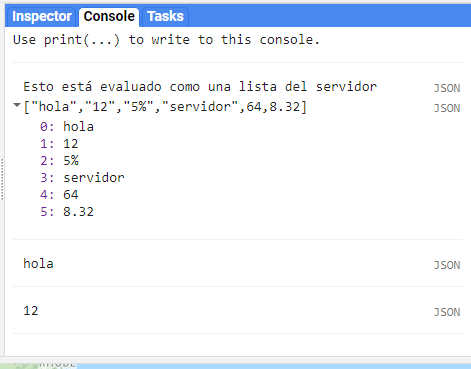
\includegraphics[width=0.7\linewidth]{Img/ej6} 

}

\caption{Salida de la consola de un objeto de tipo lista del lado del servidor.}\label{fig:f59}
\end{figure}

\hypertarget{ee.dictionary}{%
\subsection*{ee.Dictionary}\label{ee.dictionary}}
\addcontentsline{toc}{subsection}{ee.Dictionary}

\index{ee.Dictionary}
Permite enviar un objeto como diccionario al servidor. Por ejemplo (\textcolor{darkblue}{Fig.} \ref{fig:f510}).

\textcolor{darkblue}{Ejercicio 7}

\begin{Shaded}
\begin{Highlighting}[]
\CommentTok{// Se construye un diccionario de usuario con diferentes tipos de objetos}
\CommentTok{// del lado del usuario y servidor}
\ControlFlowTok{var}\NormalTok{ dicc }\OperatorTok{=}\NormalTok{ \{                                                 }
  \StringTok{\textquotesingle{}texto de usuario\textquotesingle{}}\OperatorTok{:}\StringTok{\textquotesingle{}usuario\textquotesingle{}}\OperatorTok{,}
  \StringTok{\textquotesingle{}string del servidor\textquotesingle{}}\OperatorTok{:} \KeywordTok{ee}\OperatorTok{.}\FunctionTok{String}\NormalTok{(}\StringTok{\textquotesingle{}texto de servidor \# 2\textquotesingle{}}\NormalTok{)}\OperatorTok{,}
  \StringTok{\textquotesingle{}numero de usuario\textquotesingle{}}\OperatorTok{:} \DecValTok{4}\OperatorTok{,}
  \StringTok{\textquotesingle{}numero de servidor\textquotesingle{}}\OperatorTok{:} \KeywordTok{ee}\OperatorTok{.}\FunctionTok{Number}\NormalTok{(}\FloatTok{3.1416}\NormalTok{)}\OperatorTok{,}
  \StringTok{\textquotesingle{}lista de usuario\textquotesingle{}}\OperatorTok{:}\NormalTok{ [}\DecValTok{1}\OperatorTok{,} \StringTok{\textquotesingle{}ejemplo\textquotesingle{}}\NormalTok{]}\OperatorTok{,}
  \StringTok{\textquotesingle{}lista de servidor\textquotesingle{}}\OperatorTok{:} \KeywordTok{ee}\OperatorTok{.}\FunctionTok{List}\NormalTok{([}\KeywordTok{ee}\OperatorTok{.}\FunctionTok{String}\NormalTok{(}\StringTok{\textquotesingle{}texto de servidor \# 3\textquotesingle{}}\NormalTok{)}\OperatorTok{,} 
    \KeywordTok{ee}\OperatorTok{.}\FunctionTok{Number}\NormalTok{(}\FloatTok{1.44}\NormalTok{)])}
\NormalTok{\}}\OperatorTok{;} 

\CommentTok{// Se define el diccionario de usuario anterior como ee.Dictionary del }
\CommentTok{// servidor }
\ControlFlowTok{var}\NormalTok{ diccServ }\OperatorTok{=} \KeywordTok{ee}\OperatorTok{.}\FunctionTok{Dictionary}\NormalTok{(dicc)}\OperatorTok{;}     
\end{Highlighting}
\end{Shaded}

Se puede consultar utilizando también el método \boldpurple{.get} y el nombre de la clave (\textcolor{darkblue}{Fig.} \ref{fig:f510}).

\textcolor{darkblue}{Ejercicio 7.1}

\begin{Shaded}
\begin{Highlighting}[]
\CommentTok{// Se muestra el valor que contiene la clave \textquotesingle{}lista\_de\_servidor\textquotesingle{}}
\FunctionTok{print}\NormalTok{(diccServ}\OperatorTok{.}\FunctionTok{get}\NormalTok{(}\StringTok{\textquotesingle{}lista\_de\_servidor\textquotesingle{}}\NormalTok{))}\OperatorTok{;}

\CommentTok{// Se muestra el valor que contiene el elemento \textquotesingle{}numero\_de\_usuario   }
\FunctionTok{print}\NormalTok{(diccServ}\OperatorTok{.}\FunctionTok{get}\NormalTok{(}\StringTok{\textquotesingle{}numero\_de\_usuario\textquotesingle{}}\NormalTok{))}\OperatorTok{;}        
\end{Highlighting}
\end{Shaded}

Por último, si se desea obtener las claves disponibles en un \boldpurple{ee.Dictionary} se utiliza el método \boldpurple{.keys}. Este método devuelve una lista. De igual forma, si se desea obtener los valores disponibles en un \boldpurple{ee.Dictionary} se utiliza el método \boldpurple{.values}, el cual devuelve una lista (\textcolor{darkblue}{Fig.} \ref{fig:f510}).

\textcolor{darkblue}{Ejercicio 7.2}

\begin{Shaded}
\begin{Highlighting}[]
\CommentTok{// Muestra una lista con todas las claves del ee.Dictionary}
\FunctionTok{print}\NormalTok{(}\StringTok{\textquotesingle{}claves\textquotesingle{}}\OperatorTok{,}\NormalTok{diccServ}\OperatorTok{.}\FunctionTok{keys}\NormalTok{())}\OperatorTok{;}    

\CommentTok{// Muestra una lista con todos los valores del ee.Dictionary}
\FunctionTok{print}\NormalTok{(}\StringTok{\textquotesingle{}valores\textquotesingle{}}\OperatorTok{,}\NormalTok{diccServ}\OperatorTok{.}\FunctionTok{values}\NormalTok{())}\OperatorTok{;}  
\end{Highlighting}
\end{Shaded}

\begin{figure}[H]

{\centering 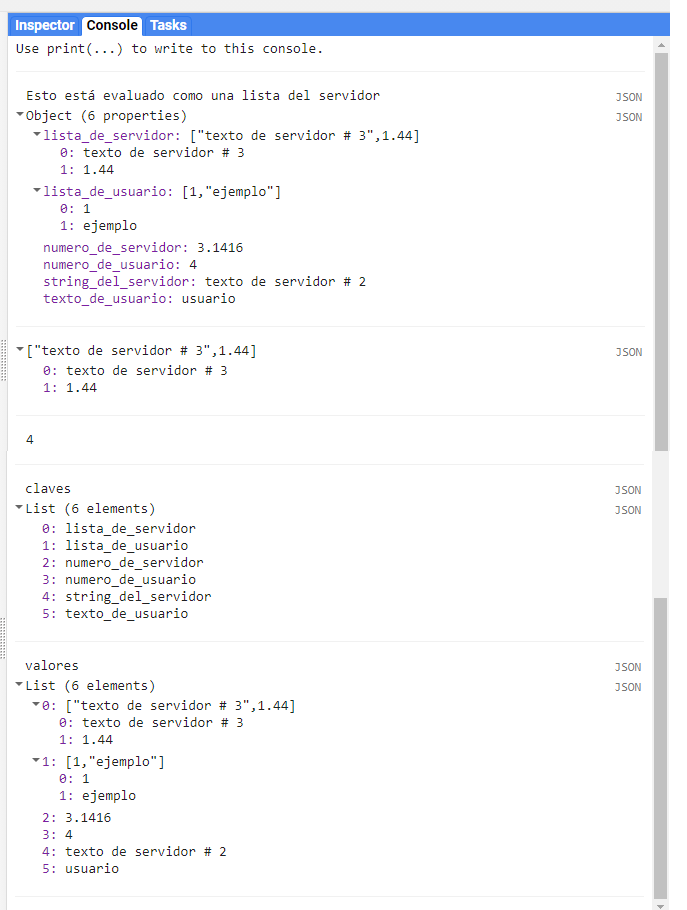
\includegraphics[width=0.95\linewidth]{Img/ej7} 

}

\caption{Salida de la consola de varios objetos de tipo diccionario del lado del servidor.}\label{fig:f510}
\end{figure}

\hypertarget{ee.date}{%
\subsection*{ee.Date}\label{ee.date}}
\addcontentsline{toc}{subsection}{ee.Date}

\index{ee.Date}
Esta es la forma en la que GEE trabaja con fechas. Hay varias formas de construir una fecha específica (\textcolor{darkblue}{Fig.} \ref{fig:f511}):

\begin{enumerate}
\def\labelenumi{\arabic{enumi}.}
\tightlist
\item
  Se puede usar un texto de usuario indicando la fecha en el siguiente formato: `AAAA-MM-DD', esta fecha obligatoriamente debe:

  \begin{itemize}
  \tightlist
  \item
    Usar la función \boldpurple{ee.Date}.
  \item
    Indicar la fecha en el orden de Año Mes Día (AAAA-MM-DD).
  \item
    Usar guiones como separadores \texttt{-}.
  \item
    Tener meses numéricos de dos dígitos (01, 02, 03, 04, 05, 06, 07, 08, 09, 10, 11, 12).
  \item
    Tener días de dos dígitos (01, 02, 03 \ldots{} 09, 10, 11 \ldots{} 30).
  \item
    Estar entre comillas.
  \end{itemize}
\item
  Usar números de usuario, en este caso se debe:

  \begin{itemize}
  \tightlist
  \item
    Usar el método \boldpurple{ee.Date.fromYMD}.
  \item
    Ingresar dentro del paréntesis el año, el mes y el día (en ese orden), separados por comas.
  \end{itemize}
\item
  Usar un texto de usuario especificando el formato, para esto se debe:

  \begin{itemize}
  \tightlist
  \item
    Usar el método \boldpurple{ee.Date.parse}.
  \item
    Especificar el formato de la fecha con la siguiente clave (AAAA = año, MM = mes, D = día).
  \item
    Especificar el tipo de separador.
  \item
    Especificar el orden en el que se ingresará el texto.
  \item
    Especificar la cantidad de dígitos esperada para cada ítem (año, mes y día).
  \item
    El formato debe estar entre comillas.
  \item
    Luego de especificar el formato, se ingresa dentro de comillas el texto a convertir a \boldpurple{ee.Date} (entre el formato y el texto debe ir una coma).
  \end{itemize}
\end{enumerate}

\begin{bluebox2}

\begin{awesomeblock}{5pt}{\faLightbulb}{darkblue}
Internamente los objetos ee.Date transforman el formato de fecha a formato UNIX (también llamado EPOCH o POSIX, que se define como la cantidad de segundos transcurridos desde la medianoche UTC del 1 de enero de 1970. Véase en la Fig. 5.11.

\end{awesomeblock}

\end{bluebox2}

\textcolor{darkblue}{Ejercicio 8}

\begin{Shaded}
\begin{Highlighting}[]
\CommentTok{// Fecha como un texto de cliente}
\ControlFlowTok{var}\NormalTok{ fechaString }\OperatorTok{=} \StringTok{\textquotesingle{}2001{-}10\textquotesingle{}}\OperatorTok{;}

\CommentTok{// Convierte la fecha de texto de cliente a ee.Date del servidor    }
\ControlFlowTok{var}\NormalTok{ fecha }\OperatorTok{=} \KeywordTok{ee}\OperatorTok{.}\FunctionTok{Date}\NormalTok{(fechaString)}\OperatorTok{;}  

\CommentTok{// Crea una ee.Date a partir de definir año, mes y día con números del }
\CommentTok{// cliente           }
\ControlFlowTok{var}\NormalTok{ fecha2 }\OperatorTok{=} \KeywordTok{ee}\OperatorTok{.}\AttributeTok{Date}\OperatorTok{.}\FunctionTok{fromYMD}\NormalTok{(}\DecValTok{2015}\OperatorTok{,}\BaseNTok{03}\OperatorTok{,}\DecValTok{28}\NormalTok{)}\OperatorTok{;} 
   
\CommentTok{// Crea una fecha a partir de un formato especificado y un texto que }
\CommentTok{// cumple con dicho formato, nótese que se especifica el orden del día }
\CommentTok{// año y mes, se especifica cada separador, y si se usan meses como texto}
\CommentTok{// deben ser las 3 primeras iniciales del mes en inglés}
\ControlFlowTok{var}\NormalTok{ fecha3 }\OperatorTok{=} \KeywordTok{ee}\OperatorTok{.}\AttributeTok{Date}\OperatorTok{.}\FunctionTok{parse}\NormalTok{(}\StringTok{\textquotesingle{}DD\_YYYY/MMM\textquotesingle{}}\OperatorTok{,} \StringTok{\textquotesingle{}14\_1827/jul\textquotesingle{}}\NormalTok{)}\OperatorTok{;} 
\end{Highlighting}
\end{Shaded}

\begin{figure}[H]

{\centering \includegraphics[width=0.95\linewidth]{Img/ej8} 

}

\caption{Salida de la consola de un objeto de tipo fecha del lado del servidor.}\label{fig:f511}
\end{figure}

\hypertarget{ee.image}{%
\subsection*{ee.Image}\label{ee.image}}
\addcontentsline{toc}{subsection}{ee.Image}

\index{ee.Image}
La definición de objetos \boldpurple{ee.Image} (imagen) habilita los métodos disponibles en GEE para el procesamiento de imágenes. Este va a ser el tipo de objetos para trabajar con cualquier elemento de tipo ráster en GEE. Más adelante se explica con mayor detalle.

\hypertarget{ee.imagecollection}{%
\subsection*{ee.ImageCollection}\label{ee.imagecollection}}
\addcontentsline{toc}{subsection}{ee.ImageCollection}

\index{ee.ImageCollection}
Las colecciones de imágenes (\emph{image collections}) están formadas por imágenes individuales (\boldpurple{ee.Image}). Más adelante se explica este tipo de objetos con mayor detalle.

\hypertarget{ee.feature}{%
\subsection*{ee.Feature}\label{ee.feature}}
\addcontentsline{toc}{subsection}{ee.Feature}

\index{ee.Feature}
Este va a ser el tipo de objetos para trabajar con cualquier objeto de tipo vector o tabla. Más adelante se explica este tipo de objeto con mayor detalle.

\hypertarget{ee.featurecollection}{%
\subsection*{ee.FeatureCollection}\label{ee.featurecollection}}
\addcontentsline{toc}{subsection}{ee.FeatureCollection}

\index{ee.FeatureCollection}
Las colecciones de vectores (\emph{feature collections}) están formadas por varios vectores (\boldpurple{ee.Feature}). Más adelante se explican estos objetos con mayor detalle.

\hypertarget{ee.algorithms}{%
\subsection*{ee.Algorithms}\label{ee.algorithms}}
\addcontentsline{toc}{subsection}{ee.Algorithms}

\index{ee.Algorithms}
Este tipo de objetos contienen algoritmos precargados en GEE. Estos algoritmos tienen una gran variedad de aplicaciones, desde operaciones sencillas como una evaluación lógica, por ejemplo, \boldpurple{ee.Algorithms.If}, hasta algoritmos de segmentación temporal de una serie de imágenes, por ejemplo, \boldpurple{ee.Algorithms.TemporalSegmentation.Ccdc}.

\hypertarget{ee.array}{%
\subsection*{ee.Array}\label{ee.array}}
\addcontentsline{toc}{subsection}{ee.Array}

\index{ee.Array}
Este tipo de objetos corresponden a arreglos multidimensionales, los cuales se pueden interpretar como matrices de más de dos dimensiones (por ejemplo, filas y columnas). Su uso más común se da en el análisis de series de tiempo o con ordenaciones espectrales. Este tipo de objetos cuentan con una serie de métodos, que se pueden consultar bajo la biblioteca de \boldpurple{ee.Array} (ver el enlace anterior).

\hypertarget{ee.classifier}{%
\subsection*{ee.Classifier}\label{ee.classifier}}
\addcontentsline{toc}{subsection}{ee.Classifier}

\index{ee.Classifier}
Este tipo de objetos corresponden a algoritmos de clasificación supervisada de datos que se encuentran precargados en GEE. Por ejemplo, se encuentra el algoritmo de random forest, disponible mediante la función \boldpurple{ee.Classifier.smileRandomForest} o MaxEnt, disponible mediante la función \boldpurple{ee.Classifier.amnhMaxent}, entre otros.

\hypertarget{ee.clusterer}{%
\subsection*{ee.Clusterer}\label{ee.clusterer}}
\addcontentsline{toc}{subsection}{ee.Clusterer}

\index{ee.Clusterer}
Este tipo de objetos corresponden a algoritmos de clasificación no supervisada de datos que se encuentran precargados en GEE. Por ejemplo, se encuentra el algoritmo de k-means, disponible mediante la función \boldpurple{ee.Clusterer.wekaKMeans} o Cobweb, disponible mediante la función \boldpurple{ee.Clusterer.wekaCobweb}.

\hypertarget{ee.filter}{%
\subsection*{ee.Filter}\label{ee.filter}}
\addcontentsline{toc}{subsection}{ee.Filter}

\index{ee.Filter}
Este tipo de objetos se utilizan para filtrar colecciones, ya sean de vectores o de imágenes. También permiten definir filtros de distintos tipos, ya sean espaciales, temporales o en función de características de las imágenes o vectores (por ejemplo, metadatos). Por último, contienen métodos para combinar filtros.

\hypertarget{ee.geometry}{%
\subsection*{ee.Geometry}\label{ee.geometry}}
\addcontentsline{toc}{subsection}{ee.Geometry}

\index{ee.Geometry}
Este tipo de objetos corresponden a distintos tipos de geometrías, que incluyen líneas, polígonos y puntos. Además, en GEE se encuentran varios métodos precargados que se pueden aplicar a este tipo de objetos como, \boldpurple{ee.Geometry.MultiPolygon.Simplify} para simplificar polígonos múltiples o \boldpurple{ee.Geometry.Polygon.area} para calcular el área de un polígono, por ejemplo.

\hypertarget{ee.join}{%
\subsection*{ee.Join}\label{ee.join}}
\addcontentsline{toc}{subsection}{ee.Join}

\index{ee.Join}
Este conjunto de métodos permite realizar uniones entre colecciones de vectores o imágenes, utilizando los campos de estos como las claves para realizar las uniones. Por ejemplo, se pueden unir dos colecciones de vectores mediante \boldpurple{ee.Join.merge} o unir los campos de una primera colección con los de una segunda mediante \boldpurple{ee.Join.inner}.

\hypertarget{ee.reducer}{%
\subsection*{ee.Reducer}\label{ee.reducer}}
\addcontentsline{toc}{subsection}{ee.Reducer}

\index{ee.Reducer}
Los reductores permiten agregar datos basados en una regla o utilizando una operación matemática determinada. Este tipo de métodos son los utilizados para generar, por ejemplo, una sola imagen a partir de varias imágenes que comparten una misma extensión espacial. El tipo de reductor define el tipo de agregación que se desea aplicar, por ejemplo, se puede reducir con una sencilla estadística (mínimo, máximo, media, moda, mediana, etc.) o con reductores más complejos (histogramas, enlistar, regresión lineal). Las reducciones se pueden realizar sobre las bandas de las imágenes o los atributos de los vectores.

\hypertarget{ee.terrain}{%
\subsection*{ee.Terrain}\label{ee.terrain}}
\addcontentsline{toc}{subsection}{ee.Terrain}

\index{ee.Terrain}
Este conjunto de métodos permite calcular algunas operaciones topográficas, a partir de un modelo digital de elevación (DEM). Por ejemplo, en GEE se encuentran los métodos \boldpurple{ee.Terrain.aspect} para calcular el aspecto o \boldpurple{ee.Terrain.slope} para calcular la pendiente.

\begin{bluebox2}

\begin{awesomeblock}{5pt}{\faLightbulb}{darkblue}
Los argumentos de cualquier método del servidor se pueden pasar de dos maneras: 1) siguiendo el orden por defecto de los argumentos del método y separando cada argumento por una coma, o 2) como un diccionario (dentro de llaves \texttt{\{\}}) indicando el nombre del argumento como la clave, seguido de dos puntos y el valor del argumento. En este último caso, también se separa cada argumento con una coma.

\end{awesomeblock}

\end{bluebox2}

\newpage

\hypertarget{ee.geometry-1}{%
\chapter{ee.Geometry}\label{ee.geometry-1}}

\index{ee.Geometry}
Las geometrías (\boldpurple{ee.Geometry}) son objetos que permiten leer y manejar formas geométricas, asociadas a un sistema de coordenadas geográficas. En GEE existen diversos tipos de geometrías que incluyen punto, multipunto, línea, multilínea, perímetro, polígono y multipolígono. Las geometrías en GEE corresponden, por defecto, a geometrías geodésicas.

\hypertarget{informaciuxf3n-y-metadatos}{%
\section{Información y metadatos}\label{informaciuxf3n-y-metadatos}}

\index{area}
\index{type}
\index{coordinates}
Dependiendo del tipo de geometría, se pueden consultar algunas características de la información y los metadatos, como el área de un polígono mediante \boldpurple{.area}, el tipo de la geometría mediante \boldpurple{.type} o las coordenadas mediante \boldpurple{.coordinates}.

\hypertarget{creaciuxf3n-de-geometruxedas}{%
\section{Creación de geometrías}\label{creaciuxf3n-de-geometruxedas}}

GEE utiliza el objeto \boldpurple{ee.Geometry} para leer y manejar formas geométricas, estas incluyen geometrías sin área, como son (\textcolor{darkblue}{Fig.} \ref{fig:f61}):

\begin{itemize}
\tightlist
\item
  Punto (\boldpurple{ee.Geometry.Point}): una coordenada en X \& Y.
\item
  Multipunto (\boldpurple{ee.Geometry.MultiPoint}): una lista de puntos.
\item
  Línea (\boldpurple{ee.Geometry.LineString}): una línea.
\item
  Multilínea (\boldpurple{ee.Geometry.MultiLineString}): una lista de líneas.
\item
  Perímetro (\boldpurple{ee.Geometry.linearRing}): un perímetro (una línea cerrada).
\end{itemize}

\textcolor{darkblue}{Ejercicio 9}

\begin{Shaded}
\begin{Highlighting}[]
\CommentTok{// Un punto definido con su coordenada  }
\ControlFlowTok{var}\NormalTok{ punto }\OperatorTok{=} \KeywordTok{ee}\OperatorTok{.}\AttributeTok{Geometry}\OperatorTok{.}\FunctionTok{Point}\NormalTok{(}\OperatorTok{{-}}\FloatTok{99.14}\OperatorTok{,} \FloatTok{19.47}\NormalTok{)}\OperatorTok{;} 

\CommentTok{// Un multipunto definido a partir de una lista de coordenadas de puntos}
\ControlFlowTok{var}\NormalTok{ MultiPunto }\OperatorTok{=} \KeywordTok{ee}\OperatorTok{.}\AttributeTok{Geometry}\OperatorTok{.}\FunctionTok{MultiPoint}\NormalTok{([     }
  \OperatorTok{{-}}\FloatTok{74.072}\OperatorTok{,} \FloatTok{4.754}\OperatorTok{,}                              
  \OperatorTok{{-}}\FloatTok{75.545}\OperatorTok{,} \FloatTok{6.285}\OperatorTok{,}                             
  \OperatorTok{{-}}\FloatTok{76.533}\OperatorTok{,} \FloatTok{3.461}\OperatorTok{,}
  \OperatorTok{{-}}\FloatTok{74.819}\OperatorTok{,} \FloatTok{10.997}\OperatorTok{,}
  \OperatorTok{{-}}\FloatTok{75.501}\OperatorTok{,} \FloatTok{10.393}\NormalTok{])}\OperatorTok{;}

\CommentTok{// Una línea definida a partir de una lista de las coordenadas de sus }
\CommentTok{// vértices}
\ControlFlowTok{var}\NormalTok{ linea }\OperatorTok{=} \KeywordTok{ee}\OperatorTok{.}\AttributeTok{Geometry}\OperatorTok{.}\FunctionTok{LineString}\NormalTok{([ }
  \OperatorTok{{-}}\FloatTok{117.08}\OperatorTok{,} \FloatTok{32.04}\OperatorTok{,}                    
  \OperatorTok{{-}}\FloatTok{104.25}\OperatorTok{,} \FloatTok{31.74}\OperatorTok{,}                    
  \OperatorTok{{-}}\FloatTok{96.69}\OperatorTok{,} \FloatTok{25.58}\OperatorTok{,}
  \OperatorTok{{-}}\FloatTok{95.99}\OperatorTok{,} \FloatTok{19.74}\OperatorTok{,}
  \OperatorTok{{-}}\FloatTok{87.2}\OperatorTok{,} \FloatTok{21.39}\OperatorTok{,}
  \OperatorTok{{-}}\FloatTok{87.2}\OperatorTok{,} \FloatTok{16.91}\OperatorTok{,}
  \OperatorTok{{-}}\FloatTok{82.28}\OperatorTok{,} \FloatTok{14.88}\OperatorTok{,}
  \OperatorTok{{-}}\FloatTok{83.15}\OperatorTok{,} \FloatTok{10.07}\OperatorTok{,}
  \OperatorTok{{-}}\FloatTok{77.35}\OperatorTok{,} \FloatTok{8.86}\OperatorTok{,}
  \OperatorTok{{-}}\FloatTok{71.55}\OperatorTok{,} \FloatTok{12.66}\NormalTok{])}\OperatorTok{;} 

\CommentTok{// Una multilínea definida a partir de una lista de líneas ee.LineString, }
\CommentTok{// que a su vez están definidas por una lista de las coordenadas de}
\CommentTok{// sus vértices}
\ControlFlowTok{var}\NormalTok{ MultiLinea }\OperatorTok{=} \KeywordTok{ee}\OperatorTok{.}\AttributeTok{Geometry}\OperatorTok{.}\FunctionTok{MultiLineString}\NormalTok{([ }
   \KeywordTok{ee}\OperatorTok{.}\AttributeTok{Geometry}\OperatorTok{.}\FunctionTok{LineString}\NormalTok{(                     }
\NormalTok{     [}\OperatorTok{{-}}\FloatTok{76.017}\OperatorTok{,} \FloatTok{26.173}\OperatorTok{,} \OperatorTok{{-}}\FloatTok{76.017}\OperatorTok{,} \FloatTok{16.173}\NormalTok{])}\OperatorTok{,}      
   \KeywordTok{ee}\OperatorTok{.}\AttributeTok{Geometry}\OperatorTok{.}\FunctionTok{LineString}\NormalTok{(                      }
\NormalTok{    [}\OperatorTok{{-}}\FloatTok{73.017}\OperatorTok{,} \FloatTok{26.173}\OperatorTok{,} \OperatorTok{{-}}\FloatTok{73.017}\OperatorTok{,} \FloatTok{16.173}\NormalTok{])}\OperatorTok{,}       
   \KeywordTok{ee}\OperatorTok{.}\AttributeTok{Geometry}\OperatorTok{.}\FunctionTok{LineString}\NormalTok{(                      }
\NormalTok{    [}\OperatorTok{{-}}\FloatTok{78.434}\OperatorTok{,} \FloatTok{20.926}\OperatorTok{,} \OperatorTok{{-}}\FloatTok{70.04}\OperatorTok{,} \FloatTok{24.401}\NormalTok{])}\OperatorTok{,}
   \KeywordTok{ee}\OperatorTok{.}\AttributeTok{Geometry}\OperatorTok{.}\FunctionTok{LineString}\NormalTok{(}
\NormalTok{    [}\OperatorTok{{-}}\FloatTok{78.434}\OperatorTok{,} \FloatTok{18.926}\OperatorTok{,} \OperatorTok{{-}}\FloatTok{70.04}\OperatorTok{,} \FloatTok{22.401}\NormalTok{])])}\OperatorTok{;}

\CommentTok{// Un perímetro definido a partir de una lista  de las coordenadas }
\CommentTok{// de los vértices}
\ControlFlowTok{var}\NormalTok{ perimetro }\OperatorTok{=} \KeywordTok{ee}\OperatorTok{.}\AttributeTok{Geometry}\OperatorTok{.}\FunctionTok{LinearRing}\NormalTok{([ }
  \OperatorTok{{-}}\FloatTok{105.732}\OperatorTok{,} \FloatTok{20.627}\OperatorTok{,}                      
  \OperatorTok{{-}}\FloatTok{109.336}\OperatorTok{,} \FloatTok{26.544}\OperatorTok{,}                      
  \OperatorTok{{-}}\FloatTok{113.291}\OperatorTok{,} \FloatTok{31.274}\OperatorTok{,}
  \OperatorTok{{-}}\FloatTok{114.829}\OperatorTok{,} \FloatTok{31.274}\OperatorTok{,}
  \OperatorTok{{-}}\FloatTok{109.468}\OperatorTok{,} \FloatTok{23.317}\NormalTok{])}\OperatorTok{;}
\end{Highlighting}
\end{Shaded}

\begin{figure}[H]

{\centering \includegraphics[width=0.95\linewidth]{Img/ej9} 

}

\caption{Visualización de los diferentes tipos de geometrías.}\label{fig:f61}
\end{figure}

También hay geometrías que tienen el componente de área, como son (\textcolor{darkblue}{Fig.} \ref{fig:f61}):

\begin{itemize}
\tightlist
\item
  Rectángulo (\boldpurple{ee.Geometry.Rectangle}): un rectángulo.
\item
  Polígono (\boldpurple{ee.Geometry.Polygon}): un polígono.
\item
  Multipolígono (\boldpurple{ee.Geometry.MultiPolygon}): una lista de polígonos.
\end{itemize}

\textcolor{darkblue}{Ejercicio 9.1}

\begin{Shaded}
\begin{Highlighting}[]
\CommentTok{// Un rectángulo definido por las coordenadas de los vértices opuestos}
\ControlFlowTok{var}\NormalTok{ rectangulo }\OperatorTok{=} \KeywordTok{ee}\OperatorTok{.}\AttributeTok{Geometry}\OperatorTok{.}\FunctionTok{Rectangle}\NormalTok{( }
  \OperatorTok{{-}}\FloatTok{104.12}\OperatorTok{,} \FloatTok{5.73}\OperatorTok{,}
  \OperatorTok{{-}}\FloatTok{88.21}\OperatorTok{,} \OperatorTok{{-}}\FloatTok{0.15}\NormalTok{)}\OperatorTok{;} 

\CommentTok{// Un polígono definido por las coordenadas de sus vértices}
\ControlFlowTok{var}\NormalTok{ poligono }\OperatorTok{=} \KeywordTok{ee}\OperatorTok{.}\AttributeTok{Geometry}\OperatorTok{.}\FunctionTok{Polygon}\NormalTok{( }
  \OperatorTok{{-}}\FloatTok{80.348}\OperatorTok{,} \OperatorTok{{-}}\FloatTok{3.36}\OperatorTok{,}
  \OperatorTok{{-}}\FloatTok{80.348}\OperatorTok{,} \OperatorTok{{-}}\FloatTok{3.36}\OperatorTok{,}
  \OperatorTok{{-}}\FloatTok{78.985}\OperatorTok{,} \OperatorTok{{-}}\FloatTok{5.113}\OperatorTok{,}
  \OperatorTok{{-}}\FloatTok{78.019}\OperatorTok{,} \OperatorTok{{-}}\FloatTok{3.228}\OperatorTok{,}
  \OperatorTok{{-}}\FloatTok{75.997}\OperatorTok{,} \OperatorTok{{-}}\FloatTok{2.394}\OperatorTok{,}
  \OperatorTok{{-}}\FloatTok{75.25}\OperatorTok{,} \OperatorTok{{-}}\FloatTok{0.901}\OperatorTok{,}
  \OperatorTok{{-}}\FloatTok{75.865}\OperatorTok{,} \FloatTok{0.11}\OperatorTok{,}
  \OperatorTok{{-}}\FloatTok{78.941}\OperatorTok{,} \FloatTok{1.428}\OperatorTok{,}
  \OperatorTok{{-}}\FloatTok{80.26}\OperatorTok{,} \FloatTok{0.725}\OperatorTok{,}
  \OperatorTok{{-}}\FloatTok{80.919}\OperatorTok{,} \OperatorTok{{-}}\FloatTok{1.911}\OperatorTok{,}
  \OperatorTok{{-}}\FloatTok{79.776}\OperatorTok{,} \OperatorTok{{-}}\FloatTok{2.614}
\NormalTok{  )}\OperatorTok{;}

\CommentTok{// Un multipolígono definido por una lista de polígonos}
\ControlFlowTok{var}\NormalTok{ Multipoligono }\OperatorTok{=} \KeywordTok{ee}\OperatorTok{.}\AttributeTok{Geometry}\OperatorTok{.}\FunctionTok{MultiPolygon}\NormalTok{([}
    \CommentTok{// El primer polígono está definido a partir de dos perímetros}
    \KeywordTok{ee}\OperatorTok{.}\AttributeTok{Geometry}\OperatorTok{.}\FunctionTok{Polygon}\NormalTok{(  }
    \CommentTok{// El primer perímetro define el polígono                }
\NormalTok{      [}\KeywordTok{ee}\OperatorTok{.}\AttributeTok{Geometry}\OperatorTok{.}\FunctionTok{LinearRing}\NormalTok{(}\OperatorTok{{-}}\FloatTok{113.53}\OperatorTok{,} \FloatTok{18.81}\OperatorTok{,} \OperatorTok{{-}}\FloatTok{101.66}\OperatorTok{,} \FloatTok{10.83}\OperatorTok{,{-}}\FloatTok{114.9}\OperatorTok{,} \FloatTok{8.93}\NormalTok{)}\OperatorTok{,}    
      \CommentTok{// El segundo perímetro define los huecos dentro del polígono}
    \KeywordTok{ee}\OperatorTok{.}\AttributeTok{Geometry}\OperatorTok{.}\FunctionTok{LinearRing}\NormalTok{(}\OperatorTok{{-}}\FloatTok{111.15}\OperatorTok{,} \FloatTok{14.52}\OperatorTok{,} \OperatorTok{{-}}\FloatTok{113.09}\OperatorTok{,} \FloatTok{11.61}\OperatorTok{,} \OperatorTok{{-}}\FloatTok{115.7}\OperatorTok{,}\FloatTok{13.58}\NormalTok{)])}\OperatorTok{,}
    \CommentTok{// El segundo polígono es una lista de coordenadas que forman un }
    \CommentTok{// triángulo}
\NormalTok{    [}\OperatorTok{{-}}\FloatTok{95.77}\OperatorTok{,} \FloatTok{17.2}\OperatorTok{,}
     \OperatorTok{{-}}\FloatTok{108.7}\OperatorTok{,} \FloatTok{17.8}\OperatorTok{,}
     \OperatorTok{{-}}\FloatTok{110.0}\OperatorTok{,} \FloatTok{8.32}\NormalTok{]}\OperatorTok{,}
    \CommentTok{// El tercer polígono es una lista de coordenadas que forman un }
    \CommentTok{// triángulo}
\NormalTok{    [}\OperatorTok{{-}}\FloatTok{105.6}\OperatorTok{,} \FloatTok{15.5}\OperatorTok{,}                
     \OperatorTok{{-}}\FloatTok{105.9}\OperatorTok{,} \FloatTok{14.2}\OperatorTok{,}
     \OperatorTok{{-}}\FloatTok{103.7}\OperatorTok{,} \FloatTok{13.2}\NormalTok{]}\OperatorTok{,}
    \CommentTok{// El cuarto polígono es una lista de coordenadas que forman un }
    \CommentTok{// triángulo}
\NormalTok{    [}\OperatorTok{{-}}\FloatTok{94.98}\OperatorTok{,} \FloatTok{14.6}\OperatorTok{,}         
     \OperatorTok{{-}}\FloatTok{95.50}\OperatorTok{,} \FloatTok{13.8}\OperatorTok{,}
     \OperatorTok{{-}}\FloatTok{93.13}\OperatorTok{,} \FloatTok{11.8}\NormalTok{]}\OperatorTok{,}
    \CommentTok{// El quinto polígono es una lista de coordenadas que forman un }
    \CommentTok{// triángulo}
\NormalTok{    [}\OperatorTok{{-}}\FloatTok{84.52}\OperatorTok{,} \FloatTok{7.62}\OperatorTok{,}         
     \OperatorTok{{-}}\FloatTok{85.84}\OperatorTok{,} \FloatTok{0.17}\OperatorTok{,}
     \OperatorTok{{-}}\FloatTok{78.10}\OperatorTok{,} \FloatTok{4.74}\NormalTok{]}\OperatorTok{,}
    \CommentTok{// El sexto polígono es una lista de coordenadas que forman un }
    \CommentTok{// triángulo}
\NormalTok{    [}\OperatorTok{{-}}\FloatTok{67.03}\OperatorTok{,} \FloatTok{11.0}\OperatorTok{,}         
     \OperatorTok{{-}}\FloatTok{67.64}\OperatorTok{,} \FloatTok{6.49}\OperatorTok{,}
     \OperatorTok{{-}}\FloatTok{62.11}\OperatorTok{,} \FloatTok{2.63}\NormalTok{]])}\OperatorTok{;}
\end{Highlighting}
\end{Shaded}

Adicionalmente, se pueden crear geometrías directamente dibujando con el cursor en el mapa. Para ello se utilizan las herramientas de la esquina superior izquierda del panel del mapa (\textcolor{darkblue}{Fig.} \ref{fig:f62}):

\begin{figure}[H]

{\centering \includegraphics[width=0.5\linewidth]{Img/geometrias} 

}

\caption{Herramienta de geometrías en la pantalla de mapa.}\label{fig:f62}
\end{figure}

A continuación se describe cada función de las herramientas de geometrías de izquierda a derecha (\textcolor{darkblue}{Fig.} \ref{fig:f63}). La primera, con el símbolo de una mano, permite moverse por el mapa. Las demás herramientas permiten crear geometrías de diferente tipo: la segunda, de tipo punto; la tercera, de tipo línea; la cuarta, de tipo polígono y la quinta, también de tipo polígono, pero se enfoca en crear rectángulos a partir de dos vértices.

\begin{figure}[H]

{\centering \includegraphics[width=0.7\linewidth]{Img/herrams} 

}

\caption{Acercamiento a las herramientas de geometrías en la pantalla de mapa.}\label{fig:f63}
\end{figure}

Todas las geometrías creadas con estas herramientas se importarán automáticamente al código y se podrán ver sobre las líneas del código (\textcolor{darkblue}{Fig.} \ref{fig:f64}):

\begin{figure}[H]

{\centering \includegraphics[width=0.7\linewidth]{Img/import} 

}

\caption{Visualización de la sección de Imports dentro de la pantalla de código.}\label{fig:f64}
\end{figure}

A estas se les puede cambiar el nombre dando clic en el nombre de la geometría importada. Además, usando la mano se pueden mover y modificar las geometrías dibujadas (\textcolor{darkblue}{Fig.} \ref{fig:f63}).

Todas las geometrías dibujadas se importarán como una sola colección, pero si se quiere tener geometrías separadas en diferentes colecciones se debe dar clic en \textbf{new layer}. Este menú aparecerá cuando se pase el cursor sobre la pestaña de geometrías dibujadas (\textcolor{darkblue}{Fig.} \ref{fig:f65}).

\begin{figure}[H]

{\centering \includegraphics[width=0.8\linewidth]{Img/nuevaGeo} 

}

\caption{Herramienta de geometrías en la pantalla de mapas.}\label{fig:f65}
\end{figure}

Pasando el cursor sobre cada una de las geometrías (en la pestaña de geometrías dibujadas) se podrá bloquear la capa para evitar modificaciones (con el candado) o cambiar la configuración (en el engranaje; \textcolor{darkblue}{Fig.} \ref{fig:f66}).

\begin{figure}[H]

{\centering \includegraphics[width=0.6\linewidth]{Img/dibujarGeo} 

}

\caption{Ubicación de las herramientas de candado y engranaje.}\label{fig:f66}
\end{figure}

Al dar clic en el engranaje se abrirá un menú donde se podrá cambiar el nombre de la geometría al escribir en la caja de texto nombrada \textbf{Name} (por defecto es `geometry'), elegir el tipo de geometría en el recuadro de \textbf{Import as} (geometría \boldpurple{ee.Geometry}, vector \boldpurple{ee.Feature} o colección de vectores \boldpurple{ee.FeatureCollection}), eliminar la geometría o cambiar el color de la geometría dibujada (al ingresar el código hexadecimal en la caja nombrada \textbf{Color} o al dar clic sobre un color del recuadro de colores) o añadir manualmente propiedades (al dar clic en el texto azul que dice \textbf{+ Property}; \textcolor{darkblue}{Fig.} \ref{fig:f67}).

\begin{figure}[H]

{\centering \includegraphics[width=0.95\linewidth]{Img/menuGeo} 

}

\caption{Ejemplo de modificación de las propiedades de las geometrías.}\label{fig:f67}
\end{figure}

\begin{bluebox2}

\begin{awesomeblock}{5pt}{\faLightbulb}{darkblue}
Recuerde que las geometrías no pueden contener propiedades o atributos, así que la opción de agregar propiedades únicamente estará disponible para objetos de tipo vector (\boldpurple{ee.Feature}) o colecciones de vectores (\boldpurple{ee.FeatureCollection})

\end{awesomeblock}

\end{bluebox2}

\hypertarget{muxe9todos-comunes}{%
\section{Métodos comunes}\label{muxe9todos-comunes}}

La mayoría de los métodos que se pueden utilizar sobre una geometría suelen ser los mismos que sobre los vectores, así que dichos métodos solo se describirán en la sección de vectores en el siguiente capítulo.

\newpage

\hypertarget{ee.feature-1}{%
\chapter{ee.Feature}\label{ee.feature-1}}

\index{ee.Feature}
Los vectores (\boldpurple{ee.Feature}) en GEE son los objetos predeterminados para leer información vectorial o de tablas.
Es importante recalcar que una \boldpurple{ee.Feature} es un vector individual, de modo que solo puede contener una sola geometría (polígono, línea, punto, multipunto, multipolígono).

\hypertarget{informaciuxf3n-y-metadatos-1}{%
\section{Información y metadatos}\label{informaciuxf3n-y-metadatos-1}}

Un vector estará compuesto por una geometría (punto, línea, polígono, multipolígono) y los atributos asociados a esa geometría (estos atributos son llamados propiedades y están almacenados en un diccionario; ver Olaya {[}2020{]} para una descripción más detallada de un vector). Para obtener información geométrica de los vectores se pueden utilizar los mismos métodos que un objeto \boldpurple{ee.Geometry}, mientras que para conocer características de las propiedades se puede utilizar el método \boldpurple{.propertyNames}.

\hypertarget{visualizaciuxf3n-de-vectores}{%
\section{Visualización de vectores}\label{visualizaciuxf3n-de-vectores}}

\index{Map.addLayer}
Las geometrías y vectores pueden ser visualizados en el mapa de GEE. El aspecto predeterminado de los vectores presenta líneas sólidas negras y un relleno semiopaco gris. Sin embargo, se puede especificar el color dentro de un diccionario en la función \boldpurple{Map.addLayer}, como código hexadecimal.

\begin{bluebox2}

\begin{awesomeblock}{5pt}{\faLightbulb}{darkblue}
Los cambios de los parámetros de visualización de los vectores no pueden hacerse en las herramientas de capa del mapa, solo pueden hacerse desde el editor de código. Para consultar el código hexadecimal del color deseado se puede acceder al siguiente enlace: \url{https://htmlcolorcodes.com/es/}

\end{awesomeblock}

\end{bluebox2}

\begin{Shaded}
\begin{Highlighting}[]
\CommentTok{// Especificar el color de la capa }
\KeywordTok{Map}\OperatorTok{.}\FunctionTok{addLayer}\NormalTok{(vector }\OperatorTok{,}\NormalTok{ \{\}}\OperatorTok{,} \StringTok{\textquotesingle{}capa por default\textquotesingle{}}\NormalTok{)}\OperatorTok{;}
\KeywordTok{Map}\OperatorTok{.}\FunctionTok{addLayer}\NormalTok{(vector}\OperatorTok{,}\NormalTok{ \{}\DataTypeTok{color}\OperatorTok{:} \StringTok{\textquotesingle{}2AF116\textquotesingle{}}\NormalTok{\}}\OperatorTok{,} \StringTok{\textquotesingle{}capa color verde\textquotesingle{}}\NormalTok{)}\OperatorTok{;}
\end{Highlighting}
\end{Shaded}

\hypertarget{creaciuxf3n-de-vectores}{%
\section{Creación de vectores}\label{creaciuxf3n-de-vectores}}

Para crear un vector desde cero es necesario definir una geometría y opcionalmente un diccionario de propiedades (atributos) asociados a esa geometría. Por ejemplo (\textcolor{darkblue}{Fig.} \ref{fig:f71}):

\textcolor{darkblue}{Ejercicio 10}

\begin{Shaded}
\begin{Highlighting}[]
\CommentTok{// Crear un polígono}
\ControlFlowTok{var}\NormalTok{ poligono }\OperatorTok{=} \KeywordTok{ee}\OperatorTok{.}\AttributeTok{Geometry}\OperatorTok{.}\FunctionTok{Polygon}\NormalTok{([}
  \OperatorTok{{-}}\FloatTok{119.24}\OperatorTok{,} \FloatTok{32.73}\OperatorTok{,}
  \OperatorTok{{-}}\FloatTok{115.02}\OperatorTok{,} \OperatorTok{{-}}\FloatTok{3.29}\OperatorTok{,}
  \OperatorTok{{-}}\FloatTok{66.5}\OperatorTok{,} \OperatorTok{{-}}\FloatTok{3.29}\OperatorTok{,}
  \OperatorTok{{-}}\FloatTok{68.43}\OperatorTok{,} \FloatTok{32.14}
\NormalTok{])}\OperatorTok{;}

\CommentTok{// Crear un vector a partir del polígono y un diccionario de atributos.}
\ControlFlowTok{var}\NormalTok{ vector }\OperatorTok{=} \KeywordTok{ee}\OperatorTok{.}\FunctionTok{Feature}\NormalTok{(}
  \CommentTok{// Polígono del vector}
\NormalTok{  poligono}\OperatorTok{,}                      
  \CommentTok{// Diccionario de atributos con 3 atributos}
\NormalTok{  \{}\DataTypeTok{anno}\OperatorTok{:} \DecValTok{1500}\OperatorTok{,}                    
  \DataTypeTok{tamaño}\OperatorTok{:} \StringTok{\textquotesingle{}865 kilometros\textquotesingle{}}\OperatorTok{,}
  \DataTypeTok{nombres}\OperatorTok{:}\NormalTok{[}\StringTok{\textquotesingle{}hugo\textquotesingle{}}\OperatorTok{,}\StringTok{\textquotesingle{}paco\textquotesingle{}}\OperatorTok{,}\StringTok{\textquotesingle{}luis\textquotesingle{}}\NormalTok{]\})}\OperatorTok{;}
\end{Highlighting}
\end{Shaded}

\hypertarget{muxe9todos-comunes-1}{%
\section{Métodos comunes}\label{muxe9todos-comunes-1}}

\hypertarget{selecciuxf3n-de-propiedades}{%
\subsection*{Selección de propiedades}\label{selecciuxf3n-de-propiedades}}
\addcontentsline{toc}{subsection}{Selección de propiedades}

\index{select}
Una vez revisados los nombres de las propiedades de un vector, se pueden seleccionar ciertos atributos mediante el método \boldpurple{.select}. Para seleccionar una única propiedad solo se requiere indicar el nombre de esta (entre comillas dentro de una lista), mientras que si se desea seleccionar varias propiedades, estas deben indicarse dentro de una lista separadas por comas.

Adicionalmente, se pueden renombrar las propiedades del vector. Para ello se inserta primero una lista que contenga las propiedades a las que se les desea cambiar el nombre, seguida de una segunda lista con los nuevos nombres. Por ejemplo (\textcolor{darkblue}{Fig.} \ref{fig:f71}):
\newpage
\textcolor{darkblue}{Ejercicio 10.1}

\begin{Shaded}
\begin{Highlighting}[]
\FunctionTok{print}\NormalTok{(vector}\OperatorTok{.}\FunctionTok{select}\NormalTok{([}\StringTok{\textquotesingle{}anno\textquotesingle{}}\NormalTok{]))}\OperatorTok{;}
\FunctionTok{print}\NormalTok{(vector}\OperatorTok{.}\FunctionTok{select}\NormalTok{([}\StringTok{\textquotesingle{}anno\textquotesingle{}}\OperatorTok{,}\StringTok{\textquotesingle{}tamaño\textquotesingle{}}\NormalTok{]))}\OperatorTok{;}
\FunctionTok{print}\NormalTok{(vector}\OperatorTok{.}\FunctionTok{select}\NormalTok{([}\StringTok{\textquotesingle{}anno\textquotesingle{}}\OperatorTok{,}\StringTok{\textquotesingle{}tamaño\textquotesingle{}}\NormalTok{]}\OperatorTok{,}\NormalTok{[}\StringTok{\textquotesingle{}year\textquotesingle{}}\OperatorTok{,}\StringTok{\textquotesingle{}southamerica\textquotesingle{}}\NormalTok{]))}\OperatorTok{;}
\end{Highlighting}
\end{Shaded}

\hypertarget{adiciuxf3n-de-nuevas-propiedades-o-modificaciuxf3n-de-propiedades-preexistentes}{%
\subsection*{Adición de nuevas propiedades o modificación de propiedades preexistentes}\label{adiciuxf3n-de-nuevas-propiedades-o-modificaciuxf3n-de-propiedades-preexistentes}}
\addcontentsline{toc}{subsection}{Adición de nuevas propiedades o modificación de propiedades preexistentes}

\index{set}
Usando el método \boldpurple{.set} se pueden modificar las propiedades preexistentes o escribir nuevas propiedades sobre el vector. En este caso, primero se indica el nombre de la clave, seguido del valor correspondiente a la clave indicada. Por ejemplo (\textcolor{darkblue}{Fig.} \ref{fig:f71}):

\textcolor{darkblue}{Ejercicio 10.2}

\begin{Shaded}
\begin{Highlighting}[]
\ControlFlowTok{var}\NormalTok{ vector1 }\OperatorTok{=}\NormalTok{ vector}\OperatorTok{.}\FunctionTok{set}\NormalTok{(}\StringTok{\textquotesingle{}tamaño\textquotesingle{}}\OperatorTok{,}\StringTok{\textquotesingle{}neotropico\textquotesingle{}}\NormalTok{)}\OperatorTok{;}
\end{Highlighting}
\end{Shaded}

\begin{figure}[H]

{\centering \includegraphics[width=0.95\linewidth]{Img/ej10} 

}

\caption{Visualización del vector creado, así como las salidas de la consola que muestran la selección de algunas propiedades o adición de una propiedad.}\label{fig:f71}
\end{figure}

\hypertarget{extracciuxf3n-y-ediciuxf3n-de-propiedades-de-vectores}{%
\subsection*{Extracción y edición de propiedades de vectores}\label{extracciuxf3n-y-ediciuxf3n-de-propiedades-de-vectores}}
\addcontentsline{toc}{subsection}{Extracción y edición de propiedades de vectores}

\index{get}
\index{select}
\index{propertyNames}
\index{toDictionary}
En este ejercicio primero se selecciona un vector para ejemplificar el uso de algunos métodos de los objetos \boldpurple{ee.Feature}. Para ello, se extrae el primer vector de una colección de vectores utilizando el método \boldpurple{.first}. Este procedimiento se verá con mayor detalle en el siguiente capítulo, en los métodos de las colecciones de vectores. A continuación, se consultarán algunas propiedades y atributos del vector seleccionado (\textcolor{darkblue}{Fig.} \ref{fig:f72}).

\begin{enumerate}
\def\labelenumi{\arabic{enumi}.}
\tightlist
\item
  Usamos el método \boldpurple{.propertyNames} para obtener una lista de los nombres de los atributos del vector.
\item
  Usamos el método \boldpurple{.toDictionary} para generar un diccionario con todos los atributos (claves) y sus valores del vector.
\item
  Usamos el método \boldpurple{.get} para obtener el valor del atributo `COAST' del vector.
\item
  Usando el método \boldpurple{.select} podemos seleccionar solamente una lista de atributos definidos, y si colocamos una segunda lista entonces los atributos de la primera lista serán renombrados con los nombres de la segunda.
\end{enumerate}

\textcolor{darkblue}{Ejercicio 11}

\begin{Shaded}
\begin{Highlighting}[]
\CommentTok{// Llamamos una capa de cuencas de alta resolución de GEE}
\CommentTok{// y se selecciona el primer vector de la colección}
\ControlFlowTok{var}\NormalTok{ cuenca }\OperatorTok{=} \KeywordTok{ee}\OperatorTok{.}\FunctionTok{Feature}\NormalTok{(}
  \KeywordTok{ee}\OperatorTok{.}\FunctionTok{FeatureCollection}\NormalTok{(}\StringTok{\textquotesingle{}WWF/HydroSHEDS/v1/Basins/hybas\_12\textquotesingle{}}\NormalTok{)}
  \OperatorTok{.}\FunctionTok{first}\NormalTok{())}\OperatorTok{;}

\CommentTok{// Extraemos los nombres de los atributos del vector como una lista}
\ControlFlowTok{var}\NormalTok{ propiedades }\OperatorTok{=}\NormalTok{ cuenca}\OperatorTok{.}\FunctionTok{propertyNames}\NormalTok{()}\OperatorTok{;}

\CommentTok{// Extraemos los atributos del vector como un diccionario}
\ControlFlowTok{var}\NormalTok{ atributos }\OperatorTok{=}\NormalTok{ cuenca}\OperatorTok{.}\FunctionTok{toDictionary}\NormalTok{()}\OperatorTok{;}

\CommentTok{// Extraemos el atributo \textquotesingle{}COAST\textquotesingle{}}
\ControlFlowTok{var}\NormalTok{ costa }\OperatorTok{=}\NormalTok{ cuenca}\OperatorTok{.}\FunctionTok{get}\NormalTok{(}\StringTok{\textquotesingle{}COAST\textquotesingle{}}\NormalTok{)}\OperatorTok{;}

\CommentTok{// Extraemos el atributo \textquotesingle{}COAST\textquotesingle{} y lo renombramos como \textquotesingle{}costa maritima\textquotesingle{}}
\ControlFlowTok{var}\NormalTok{ renombre }\OperatorTok{=}\NormalTok{ cuenca}\OperatorTok{.}\FunctionTok{select}\NormalTok{([}\StringTok{\textquotesingle{}COAST\textquotesingle{}}\NormalTok{]}\OperatorTok{,}\NormalTok{[}\StringTok{\textquotesingle{}costa maritima\textquotesingle{}}\NormalTok{])}\OperatorTok{;}
\end{Highlighting}
\end{Shaded}

\begin{figure}[H]

{\centering \includegraphics[width=0.95\linewidth]{Img/ej11} 

}

\caption{Salida de la consola de las propiedades del vector de cuenca, así como de la selección de algunas de sus propiedades.}\label{fig:f72}
\end{figure}

\hypertarget{intersecciuxf3n-con-otros-vectores}{%
\subsection*{Intersección con otros vectores}\label{intersecciuxf3n-con-otros-vectores}}
\addcontentsline{toc}{subsection}{Intersección con otros vectores}

\index{intersection}
Se pueden realizar cortes de un vector para quedarse con el área específica que intersecta otro vector utilizando el método \boldpurple{.intersection}. Por ejemplo (\textcolor{darkblue}{Fig.} \ref{fig:f73}):

\textcolor{darkblue}{Ejercicio 12}

\begin{Shaded}
\begin{Highlighting}[]
\CommentTok{// Crear dos vectores rectangulares}
\ControlFlowTok{var}\NormalTok{ rectangulo1 }\OperatorTok{=} \KeywordTok{ee}\OperatorTok{.}\FunctionTok{Feature}\NormalTok{(}\KeywordTok{ee}\OperatorTok{.}\AttributeTok{Geometry}\OperatorTok{.}\FunctionTok{Rectangle}\NormalTok{(}\OperatorTok{{-}}\FloatTok{92.0}\OperatorTok{,}\FloatTok{10.6}\OperatorTok{,{-}}\FloatTok{82.0}\OperatorTok{,}\FloatTok{20.7}\NormalTok{))}\OperatorTok{;}
\ControlFlowTok{var}\NormalTok{ rectangulo2 }\OperatorTok{=} \KeywordTok{ee}\OperatorTok{.}\FunctionTok{Feature}\NormalTok{(}\KeywordTok{ee}\OperatorTok{.}\AttributeTok{Geometry}\OperatorTok{.}\FunctionTok{Rectangle}\NormalTok{(}\OperatorTok{{-}}\FloatTok{86.03}\OperatorTok{,}\FloatTok{15.6}\OperatorTok{,{-}}\FloatTok{100.0}\OperatorTok{,}\FloatTok{40.7}\NormalTok{))}\OperatorTok{;}

\CommentTok{// Intersección}
\ControlFlowTok{var}\NormalTok{ interseccion }\OperatorTok{=}\NormalTok{ rectangulo1}\OperatorTok{.}\FunctionTok{intersection}\NormalTok{(rectangulo2)}\OperatorTok{;}
\end{Highlighting}
\end{Shaded}

\begin{bluebox2}

\begin{awesomeblock}{5pt}{\faLightbulb}{darkblue}
Al realizar una intersección, el vector resultante heredará los atributos del vector al que se le aplicó dicho método (es decir, el objeto que queda del lado izquierdo del método \boldpurple{.intersection}).

\end{awesomeblock}

\end{bluebox2}

\hypertarget{creaciuxf3n-de-un-buffer}{%
\subsection*{Creación de un buffer}\label{creaciuxf3n-de-un-buffer}}
\addcontentsline{toc}{subsection}{Creación de un buffer}

\index{buffer}
Para realizar un buffer a partir de un vector se utiliza el método \boldpurple{.buffer}, en el cual hay que indicar el valor en metros del tamaño del buffer y el error máximo aceptado (\textcolor{darkblue}{Fig.} \ref{fig:f73}).

\textcolor{darkblue}{Ejercicio 12.1}

\begin{Shaded}
\begin{Highlighting}[]
\CommentTok{// Crear un vector de un  punto}
\ControlFlowTok{var}\NormalTok{ punto }\OperatorTok{=} \KeywordTok{ee}\OperatorTok{.}\FunctionTok{Feature}\NormalTok{(}\KeywordTok{ee}\OperatorTok{.}\AttributeTok{Geometry}\OperatorTok{.}\FunctionTok{Point}\NormalTok{(}\OperatorTok{{-}}\FloatTok{105.24}\OperatorTok{,} \OperatorTok{{-}}\FloatTok{2.73}\NormalTok{))}\OperatorTok{;}

\CommentTok{// Calcular un buffer de 500 km alrededor del punto}
\ControlFlowTok{var}\NormalTok{ bufferPol }\OperatorTok{=}\NormalTok{ punto}\OperatorTok{.}\FunctionTok{buffer}\NormalTok{(}\DecValTok{500000}\OperatorTok{,} \FloatTok{0.1}\NormalTok{)}\OperatorTok{;}
\end{Highlighting}
\end{Shaded}

\hypertarget{cuxe1lculo-de-uxe1rea}{%
\subsection*{Cálculo de área}\label{cuxe1lculo-de-uxe1rea}}
\addcontentsline{toc}{subsection}{Cálculo de área}

\index{area}
Para calcular el área de un vector se utiliza el método \boldpurple{.area}. En este caso hay que definir el valor máximo de error aceptado. El área siempre se calcula en metros cuadrados (\textcolor{darkblue}{Fig.} \ref{fig:f73}).

\textcolor{darkblue}{Ejercicio 12.2}

\begin{Shaded}
\begin{Highlighting}[]
\CommentTok{// Calcular el área del buffer}
\ControlFlowTok{var}\NormalTok{ area }\OperatorTok{=}\NormalTok{ bufferPol}\OperatorTok{.}\FunctionTok{area}\NormalTok{(}\FloatTok{0.1}\NormalTok{)}\OperatorTok{;}
\end{Highlighting}
\end{Shaded}

\hypertarget{cuxe1lculo-de-peruxedmetro}{%
\subsection*{Cálculo de perímetro}\label{cuxe1lculo-de-peruxedmetro}}
\addcontentsline{toc}{subsection}{Cálculo de perímetro}

\index{perimeter}
Podemos calcular el perímetro de un vector usando el método \boldpurple{.perimeter}, que hace el cálculo en metros (\textcolor{darkblue}{Fig.} \ref{fig:f73}).

\textcolor{darkblue}{Ejercicio 12.3}

\begin{Shaded}
\begin{Highlighting}[]
\CommentTok{// Calcular el perímetro del buffer}
\ControlFlowTok{var}\NormalTok{ perimetro }\OperatorTok{=}\NormalTok{ interseccion}\OperatorTok{.}\FunctionTok{perimeter}\NormalTok{()}\OperatorTok{;}
\end{Highlighting}
\end{Shaded}

\hypertarget{disoluciuxf3n-de-poluxedgonos}{%
\subsection*{Disolución de polígonos}\label{disoluciuxf3n-de-poluxedgonos}}
\addcontentsline{toc}{subsection}{Disolución de polígonos}

\index{dissolve}
El método \boldpurple{.dissolve} une todas las geometrías que se intersectan de un vector en un solo polígono y si no se intersectan, genera un multipolígono (\textcolor{darkblue}{Fig.} \ref{fig:f73}).

\textcolor{darkblue}{Ejercicio 12.4}

\begin{Shaded}
\begin{Highlighting}[]
\CommentTok{// Crear un vector de multipolígono}
\ControlFlowTok{var}\NormalTok{ multi }\OperatorTok{=} \KeywordTok{ee}\OperatorTok{.}\FunctionTok{Feature}\NormalTok{(}\KeywordTok{ee}\OperatorTok{.}\AttributeTok{Geometry}\OperatorTok{.}\FunctionTok{MultiPolygon}\NormalTok{(}
\NormalTok{            [[[[}\OperatorTok{{-}}\DecValTok{137}\OperatorTok{,} \DecValTok{20}\NormalTok{]}\OperatorTok{,}\NormalTok{ [}\OperatorTok{{-}}\DecValTok{128}\OperatorTok{,} \DecValTok{9}\NormalTok{]}\OperatorTok{,}\NormalTok{ [}\OperatorTok{{-}}\DecValTok{116}\OperatorTok{,} \DecValTok{15}\NormalTok{]}\OperatorTok{,}\NormalTok{[}\OperatorTok{{-}}\DecValTok{124}\OperatorTok{,} \DecValTok{25}\NormalTok{]]]}\OperatorTok{,}
\NormalTok{             [[[}\OperatorTok{{-}}\DecValTok{123}\OperatorTok{,} \DecValTok{28}\NormalTok{]}\OperatorTok{,}\NormalTok{ [}\OperatorTok{{-}}\DecValTok{129}\OperatorTok{,} \DecValTok{30}\NormalTok{]}\OperatorTok{,}\NormalTok{ [}\OperatorTok{{-}}\DecValTok{139}\OperatorTok{,} \DecValTok{5}\NormalTok{]]]}\OperatorTok{,}
\NormalTok{             [[[}\OperatorTok{{-}}\DecValTok{113}\OperatorTok{,} \DecValTok{19}\NormalTok{]}\OperatorTok{,}\NormalTok{ [}\OperatorTok{{-}}\DecValTok{143}\OperatorTok{,} \DecValTok{18}\NormalTok{]}\OperatorTok{,}\NormalTok{ [}\OperatorTok{{-}}\DecValTok{123}\OperatorTok{,} \DecValTok{4}\NormalTok{]]]}\OperatorTok{,}
\NormalTok{             [[[}\OperatorTok{{-}}\DecValTok{133}\OperatorTok{,} \DecValTok{1}\NormalTok{]}\OperatorTok{,}\NormalTok{ [}\OperatorTok{{-}}\DecValTok{118}\OperatorTok{,} \DecValTok{2}\NormalTok{]}\OperatorTok{,}\NormalTok{ [}\OperatorTok{{-}}\DecValTok{116}\OperatorTok{,} \DecValTok{24}\NormalTok{]]]}\OperatorTok{,}
\NormalTok{             [[[}\OperatorTok{{-}}\DecValTok{109}\OperatorTok{,} \DecValTok{5}\NormalTok{]}\OperatorTok{,}\NormalTok{ [}\OperatorTok{{-}}\DecValTok{103}\OperatorTok{,} \DecValTok{10}\NormalTok{]}\OperatorTok{,}\NormalTok{ [}\OperatorTok{{-}}\DecValTok{147}\OperatorTok{,} \DecValTok{9}\NormalTok{]]]}\OperatorTok{,}
\NormalTok{             [[[}\OperatorTok{{-}}\DecValTok{110}\OperatorTok{,} \DecValTok{14}\NormalTok{]}\OperatorTok{,}\NormalTok{ [}\OperatorTok{{-}}\DecValTok{160}\OperatorTok{,} \DecValTok{12}\NormalTok{]}\OperatorTok{,}\NormalTok{ [}\OperatorTok{{-}}\DecValTok{161}\OperatorTok{,} \DecValTok{7}\NormalTok{]]]}\OperatorTok{,}
\NormalTok{             [[[}\OperatorTok{{-}}\DecValTok{117}\OperatorTok{,} \OperatorTok{{-}}\DecValTok{1}\NormalTok{]}\OperatorTok{,}\NormalTok{ [}\OperatorTok{{-}}\DecValTok{117}\OperatorTok{,} \OperatorTok{{-}}\DecValTok{2}\NormalTok{]}\OperatorTok{,}\NormalTok{ [}\OperatorTok{{-}}\DecValTok{136}\OperatorTok{,} \OperatorTok{{-}}\DecValTok{9}\NormalTok{]]]}\OperatorTok{,}
\NormalTok{             [[[}\OperatorTok{{-}}\DecValTok{121}\OperatorTok{,} \OperatorTok{{-}}\DecValTok{1}\NormalTok{]}\OperatorTok{,}\NormalTok{ [}\OperatorTok{{-}}\DecValTok{123}\OperatorTok{,} \OperatorTok{{-}}\DecValTok{1}\NormalTok{]}\OperatorTok{,}\NormalTok{ [}\OperatorTok{{-}}\DecValTok{126}\OperatorTok{,} \OperatorTok{{-}}\DecValTok{18}\NormalTok{]]]]))}\OperatorTok{;}
\CommentTok{// Disolver sus geometrías}
\ControlFlowTok{var}\NormalTok{ disuelto }\OperatorTok{=} \KeywordTok{ee}\OperatorTok{.}\FunctionTok{Feature}\NormalTok{(multi}\OperatorTok{.}\FunctionTok{dissolve}\NormalTok{(}\FloatTok{0.1}\NormalTok{))}\OperatorTok{;}
\end{Highlighting}
\end{Shaded}

\hypertarget{uniuxf3n-de-vectores}{%
\subsection*{Unión de vectores}\label{uniuxf3n-de-vectores}}
\addcontentsline{toc}{subsection}{Unión de vectores}

\index{union}
El método \boldpurple{.union} permite fusionar las geometrías de dos vectores en una sola geometría de un vector. Las geometrías que están intersectadas serán disueltas y las que no lo estén se convertirán en un multipolígono (\textcolor{darkblue}{Fig.} \ref{fig:f73}).

\textcolor{darkblue}{Ejercicio 12.5}

\begin{Shaded}
\begin{Highlighting}[]
\CommentTok{// Unir geometrías del buffer y un rectángulo }
\ControlFlowTok{var}\NormalTok{ union }\OperatorTok{=}\NormalTok{ rectangulo2}\OperatorTok{.}\FunctionTok{union}\NormalTok{(bufferPol)}
\end{Highlighting}
\end{Shaded}

\begin{figure}[H]

{\centering \includegraphics[width=0.95\linewidth]{Img/ej12} 

}

\caption{Visualización de la unión de diferentes geometrías, así como la salida de la consola de la intersección, área y perímetro calculados.}\label{fig:f73}
\end{figure}

\newpage

\hypertarget{ee.featurecollection-1}{%
\chapter{ee.FeatureCollection}\label{ee.featurecollection-1}}

\index{ee.FeatureCollection}
Las colecciones de vectores (\boldpurple{ee.FeatureCollection}) son objetos de GEE que contienen un conjunto de vectores, de modo que pueden contener objetos \boldpurple{ee.Feature} con geometrías diferentes (polígono, línea, punto, multipunto, multipolígono). La mayoría de los acervos de información vectorial disponibles en GEE van a ser definidos como colecciones de vectores. Para el manejo de varios vectores se recomienda utilizar esta estructura, en lugar de listas u otro tipo de objetos, ya que esto facilita ejecutar operaciones sobre todo el conjunto de vectores. Por ejemplo (\textcolor{darkblue}{Fig.} \ref{fig:f81}):

\begin{bluebox2}

\begin{awesomeblock}{5pt}{\faLightbulb}{darkblue}
GEE ofrece un catálogo de colecciones de vectores que se puede buscar en la barra de búsqueda. Estas colecciones de vectores se llaman tablas (\emph{tables}).
La búsqueda de información vectorial en los acervos de GEE es más difícil que la búsqueda de imágenes. Eso ocurre porque a pesar de que hay mucha información vectorial disponible (compartida por usuarios), solo está indexada la información compartida por Google.

\end{awesomeblock}

\end{bluebox2}

\textcolor{darkblue}{Ejercicio 13}

\begin{Shaded}
\begin{Highlighting}[]
\CommentTok{// En el buscador se busca una tabla de países \textquotesingle{}countries\textquotesingle{} y se escribe }
\CommentTok{// el ID de la tabla, en este caso es una colección de vectores del }
\CommentTok{// Departamento de Estado de Estados Unidos, que contiene las divisiones }
\CommentTok{// políticas de los países del mundo  }
\ControlFlowTok{var}\NormalTok{ paises }\OperatorTok{=} \KeywordTok{ee}\OperatorTok{.}\FunctionTok{FeatureCollection}\NormalTok{(}\StringTok{\textquotesingle{}USDOS/LSIB\_SIMPLE/2017\textquotesingle{}}\NormalTok{)}\OperatorTok{;}
\end{Highlighting}
\end{Shaded}

\begin{figure}[H]

{\centering \includegraphics[width=0.95\linewidth]{Img/ej13} 

}

\caption{Visualización de la colección de vectores con los límites internacionales, así como su salida en la consola.}\label{fig:f81}
\end{figure}

\hypertarget{informaciuxf3n-y-metadatos-2}{%
\section{Información y metadatos}\label{informaciuxf3n-y-metadatos-2}}

\index{size}
\index{limit}
En las colecciones de vectores se ubican los metadatos e información de todos los vectores que contienen. Gracias a ello se puede utilizar esta información para filtrar y utilizar únicamente los vectores que cumplen con ciertos criterios. Algunos de los métodos que permiten examinar una colección de vectores incluyen \boldpurple{.size} y \boldpurple{.limit} (\textcolor{darkblue}{Fig.} \ref{fig:f82}).

\textcolor{darkblue}{Ejercicio 14}

\begin{Shaded}
\begin{Highlighting}[]
\CommentTok{// Llamamos una capa de cuencas de alta resolución de GEE}
\ControlFlowTok{var}\NormalTok{ cuencas }\OperatorTok{=} \KeywordTok{ee}\OperatorTok{.}\FunctionTok{FeatureCollection}\NormalTok{(}\StringTok{\textquotesingle{}WWF/HydroSHEDS/v1/Basins/hybas\_12\textquotesingle{}}\NormalTok{)}\OperatorTok{;}

\CommentTok{// Cantidad de vectores en la colección (1034083)}
\ControlFlowTok{var}\NormalTok{ cantidad }\OperatorTok{=}\NormalTok{cuencas}\OperatorTok{.}\FunctionTok{size}\NormalTok{()}\OperatorTok{;} 
\CommentTok{// Seleccionamos solo los primeros 50 vectores}
\ControlFlowTok{var}\NormalTok{ primeras50cuencas}\OperatorTok{=}\NormalTok{ cuencas}\OperatorTok{.}\FunctionTok{limit}\NormalTok{(}\DecValTok{50}\NormalTok{)}\OperatorTok{;} 
\CommentTok{// Este comando resultará en un error porque excede los 5000 vectores}
\FunctionTok{print}\NormalTok{(cuencas)}\OperatorTok{;} 

\CommentTok{// Esta capa contiene todos los vectores 1034083. Nótese que en el mapa }
\CommentTok{// sí se pueden proyectar más de 5000 vectores, aunque esta capa es un }
\CommentTok{// poco pesada }
\KeywordTok{Map}\OperatorTok{.}\FunctionTok{addLayer}\NormalTok{(cuencas}\OperatorTok{,}\NormalTok{\{\}}\OperatorTok{,}\StringTok{\textquotesingle{}todas las cuencas\textquotesingle{}}\NormalTok{)}\OperatorTok{;}
\CommentTok{// Esta capa solo contiene las primeras 1000 cuencas y carga mucho más }
\CommentTok{// rápido (Noroccidente de África)}
\KeywordTok{Map}\OperatorTok{.}\FunctionTok{addLayer}\NormalTok{(cuencas}\OperatorTok{.}\FunctionTok{limit}\NormalTok{(}\DecValTok{1000}\NormalTok{)}\OperatorTok{,}\NormalTok{\{}\DataTypeTok{color}\OperatorTok{:}\StringTok{\textquotesingle{}00ff00\textquotesingle{}}\NormalTok{\}}\OperatorTok{,}\StringTok{\textquotesingle{}1000 cuencas filtradas\textquotesingle{}}\NormalTok{)}\OperatorTok{;}
\end{Highlighting}
\end{Shaded}

\begin{figure}[H]

{\centering \includegraphics[width=0.95\linewidth]{Img/ej14} 

}

\caption{Visualización de las primeras 1000 cuencas, así como su salida en la consola.}\label{fig:f82}
\end{figure}

\begin{bluebox2}

\begin{awesomeblock}{5pt}{\faLightbulb}{darkblue}
Al usar \boldpurple{print} con las colecciones de vectores, la consola puede mostrar un máximo de 5000 vectores. En caso que uno necesite usar \boldpurple{print} en una colección de más de 5000 vectores, será necesario filtrar la colección previamente. Otra opción es limitar la cantidad de vectores que se vayan a mostrar. Para ello se puede usar el método \boldpurple{.limit}, el cual permite especificar la cantidad de vectores que queremos ver (siempre que sean \textless= 5000; \textcolor{darkblue}{Fig.} \ref{fig:f82}).

\end{awesomeblock}

\end{bluebox2}

\hypertarget{creaciuxf3n-de-colecciones-de-vectores}{%
\section{Creación de colecciones de vectores}\label{creaciuxf3n-de-colecciones-de-vectores}}

Una colección de vectores se define a partir del método \boldpurple{ee.FeatureCollection} y puede contener geometrías, vectores o inclusive otra colección de vectores. Una colección de vectores puede contener un solo vector o una sola geometría y sus elementos pueden tener o no atributos. Por ejemplo (\textcolor{darkblue}{Fig.} \ref{fig:f83}, \ref{fig:f84}):

\textcolor{darkblue}{Ejercicio 15}

\begin{Shaded}
\begin{Highlighting}[]
\CommentTok{// Crear una colección de vectores con un solo punto, sin atributos }
\ControlFlowTok{var}\NormalTok{ coleccion }\OperatorTok{=} \KeywordTok{ee}\OperatorTok{.}\FunctionTok{FeatureCollection}\NormalTok{(}\KeywordTok{ee}\OperatorTok{.}\AttributeTok{Geometry}\OperatorTok{.}\FunctionTok{Point}\NormalTok{(}\FloatTok{16.37}\OperatorTok{,} \FloatTok{48.225}\NormalTok{))}\OperatorTok{;}
\end{Highlighting}
\end{Shaded}

\begin{figure}[H]

{\centering \includegraphics[width=0.8\linewidth]{Img/ej15} 

}

\caption{Visualización de una colección de vectores con un único objeto de geometría de tipo punto.}\label{fig:f83}
\end{figure}

\textcolor{darkblue}{Ejercicio 16}

\begin{Shaded}
\begin{Highlighting}[]
\CommentTok{// Información adicional para el ejemplo, creación de }
\CommentTok{// distintos vectores (ee.Feature),}
\CommentTok{// cada cual con diferentes tipos de geometrías y distintos}
\CommentTok{// atributos, esto para mostrar que una ee.FeatureCollection }
\CommentTok{// no requiere que todos sus elementos (ee.Feature)}
\CommentTok{// tengan los mismos atributos ni geometrías}
\ControlFlowTok{var}\NormalTok{ Punto }\OperatorTok{=} \KeywordTok{ee}\OperatorTok{.}\FunctionTok{Feature}\NormalTok{(}\KeywordTok{ee}\OperatorTok{.}\AttributeTok{Geometry}\OperatorTok{.}\FunctionTok{Point}\NormalTok{(}\OperatorTok{{-}}\FloatTok{99.1362}\OperatorTok{,} \FloatTok{19.4352}\NormalTok{)}\OperatorTok{,}
\NormalTok{    \{}\DataTypeTok{pais}\OperatorTok{:}\StringTok{\textquotesingle{}Mexico\textquotesingle{}}\OperatorTok{,}\DataTypeTok{capital}\OperatorTok{:}\StringTok{\textquotesingle{}cdmx\textquotesingle{}}\NormalTok{\})}\OperatorTok{;}

\ControlFlowTok{var}\NormalTok{ Multipunto }\OperatorTok{=} \KeywordTok{ee}\OperatorTok{.}\FunctionTok{Feature}\NormalTok{(}
\KeywordTok{ee}\OperatorTok{.}\AttributeTok{Geometry}\OperatorTok{.}\FunctionTok{MultiPoint}\NormalTok{([}\OperatorTok{{-}}\FloatTok{90.496}\OperatorTok{,} \FloatTok{14.605}\OperatorTok{,} \OperatorTok{{-}}\FloatTok{88.717}\OperatorTok{,} \FloatTok{17.245}\OperatorTok{,}                            
                        \OperatorTok{{-}}\FloatTok{87.157}\OperatorTok{,} \FloatTok{14.094}\OperatorTok{,} \OperatorTok{{-}}\FloatTok{89.2275}\OperatorTok{,} \FloatTok{13.6937}\OperatorTok{,}
                        \OperatorTok{{-}}\FloatTok{86.273}\OperatorTok{,} \FloatTok{12.115}\OperatorTok{,} \OperatorTok{{-}}\FloatTok{84.097}\OperatorTok{,} \FloatTok{9.958}\OperatorTok{,}
                        \OperatorTok{{-}}\FloatTok{79.527}\OperatorTok{,} \FloatTok{8.983}\NormalTok{])}\OperatorTok{,}
\NormalTok{    \{}\DataTypeTok{pais}\OperatorTok{:}\NormalTok{ [}\StringTok{\textquotesingle{}Guatemala\textquotesingle{}}\OperatorTok{,} \StringTok{\textquotesingle{}Belice\textquotesingle{}}\OperatorTok{,} 
        \StringTok{\textquotesingle{}Honduras\textquotesingle{}}\OperatorTok{,} \StringTok{\textquotesingle{}El Salvador\textquotesingle{}}\OperatorTok{,} 
        \StringTok{\textquotesingle{}Nicaragua\textquotesingle{}}\OperatorTok{,} \StringTok{\textquotesingle{}Costa Rica\textquotesingle{}}\OperatorTok{,} 
        \StringTok{\textquotesingle{}Panama\textquotesingle{}}\NormalTok{]}\OperatorTok{,}
    \DataTypeTok{capital}\OperatorTok{:}\NormalTok{    [}\StringTok{\textquotesingle{}cdad. de Guatemala\textquotesingle{}}\OperatorTok{,} \StringTok{\textquotesingle{}Belmopan\textquotesingle{}}\OperatorTok{,} 
        \StringTok{\textquotesingle{}Tegucigalpa\textquotesingle{}}\OperatorTok{,} \StringTok{\textquotesingle{}San Salvador\textquotesingle{}}\OperatorTok{,} 
        \StringTok{\textquotesingle{}Managua\textquotesingle{}}\OperatorTok{,} \StringTok{\textquotesingle{}San Jose\textquotesingle{}}\OperatorTok{,} 
        \StringTok{\textquotesingle{}cdad. de Panama\textquotesingle{}}\NormalTok{]\})}\OperatorTok{;}

\ControlFlowTok{var}\NormalTok{ linea }\OperatorTok{=} \KeywordTok{ee}\OperatorTok{.}\FunctionTok{Feature}\NormalTok{(}\KeywordTok{ee}\OperatorTok{.}\AttributeTok{Geometry}\OperatorTok{.}\FunctionTok{LineString}\NormalTok{([}\OperatorTok{{-}}\FloatTok{66.865}\OperatorTok{,} \FloatTok{10.479}\OperatorTok{,}                    
                            \OperatorTok{{-}}\FloatTok{74.072}\OperatorTok{,}\FloatTok{4.732}\NormalTok{])}\OperatorTok{,}
\NormalTok{        \{}\DataTypeTok{pais}\OperatorTok{:} \StringTok{\textquotesingle{}Venezuela {-} Colombia\textquotesingle{}}\OperatorTok{,} 
      \DataTypeTok{capital}\OperatorTok{:} \StringTok{\textquotesingle{}Caracas {-} Bogota\textquotesingle{}}\NormalTok{\})}\OperatorTok{;} 

\ControlFlowTok{var}\NormalTok{ Multilinea }\OperatorTok{=} \KeywordTok{ee}\OperatorTok{.}\FunctionTok{Feature}\NormalTok{(}\KeywordTok{ee}\OperatorTok{.}\AttributeTok{Geometry}\OperatorTok{.}\FunctionTok{MultiLineString}\NormalTok{([  }
    \KeywordTok{ee}\OperatorTok{.}\AttributeTok{Geometry}\OperatorTok{.}\FunctionTok{LineString}\NormalTok{([}\OperatorTok{{-}}\FloatTok{76.803}\OperatorTok{,} \FloatTok{18.021}\OperatorTok{,} \OperatorTok{{-}}\FloatTok{82.362}\OperatorTok{,} \FloatTok{23.121}\NormalTok{])}\OperatorTok{,}      
    \KeywordTok{ee}\OperatorTok{.}\AttributeTok{Geometry}\OperatorTok{.}\FunctionTok{LineString}\NormalTok{([}\OperatorTok{{-}}\FloatTok{72.31}\OperatorTok{,} \FloatTok{18.69}\OperatorTok{,} \OperatorTok{{-}}\FloatTok{69.98}\OperatorTok{,} \FloatTok{18.44}\NormalTok{])}\OperatorTok{,}        
    \KeywordTok{ee}\OperatorTok{.}\AttributeTok{Geometry}\OperatorTok{.}\FunctionTok{LineString}\NormalTok{([}\OperatorTok{{-}}\FloatTok{66.103}\OperatorTok{,} \FloatTok{18.4597}\OperatorTok{,} \OperatorTok{{-}}\FloatTok{61.8558}\OperatorTok{,} \FloatTok{17.1315}\NormalTok{])}\OperatorTok{,}
    \KeywordTok{ee}\OperatorTok{.}\AttributeTok{Geometry}\OperatorTok{.}\FunctionTok{LineString}\NormalTok{([}\OperatorTok{{-}}\FloatTok{55.165}\OperatorTok{,} \FloatTok{5.861}\OperatorTok{,} \OperatorTok{{-}}\FloatTok{58.149}\OperatorTok{,} \FloatTok{6.822}\NormalTok{])])}\OperatorTok{,}
\NormalTok{    \{}\DataTypeTok{pais}\OperatorTok{:}\NormalTok{  [}\StringTok{\textquotesingle{}Jamaica {-} Cuba\textquotesingle{}}\OperatorTok{,}
            \StringTok{\textquotesingle{}Haiti {-} Republica Dominicana\textquotesingle{}}\OperatorTok{,}
            \StringTok{\textquotesingle{}Puerto Rico {-} Antigua y Barbuda\textquotesingle{}}\OperatorTok{,}
            \StringTok{\textquotesingle{}Surinam {-} Guyana\textquotesingle{}}\NormalTok{]}\OperatorTok{,}
    \DataTypeTok{capital}\OperatorTok{:}\NormalTok{[}\StringTok{\textquotesingle{}Kingston {-} La Habana\textquotesingle{}}\OperatorTok{,}
            \StringTok{\textquotesingle{}Puerto Principe {-} Santo Domingo\textquotesingle{}}\OperatorTok{,}
            \StringTok{\textquotesingle{}San Juan {-} saint John\textquotesingle{}}\OperatorTok{,}
            \StringTok{\textquotesingle{}Paramaribo {-} Georgetown\textquotesingle{}}\NormalTok{]\})}\OperatorTok{;}

\ControlFlowTok{var}\NormalTok{ perimetro }\OperatorTok{=} \KeywordTok{ee}\OperatorTok{.}\FunctionTok{Feature}\NormalTok{(}\KeywordTok{ee}\OperatorTok{.}\AttributeTok{Geometry}\OperatorTok{.}\FunctionTok{LinearRing}\NormalTok{([}\OperatorTok{{-}}\FloatTok{79.354}\OperatorTok{,}\FloatTok{27.32}\OperatorTok{,}
                                   \OperatorTok{{-}}\FloatTok{79.332}\OperatorTok{,} \FloatTok{23.661}\OperatorTok{,}
                                   \OperatorTok{{-}}\FloatTok{74.19}\OperatorTok{,} \FloatTok{21.161}\OperatorTok{,}
                                 \OperatorTok{{-}}\FloatTok{72.235}\OperatorTok{,} \FloatTok{23.165}\OperatorTok{,}
                                   \OperatorTok{{-}}\FloatTok{78.039}\OperatorTok{,} \FloatTok{27.859}\NormalTok{])}\OperatorTok{,}
\NormalTok{        \{}\DataTypeTok{pais}\OperatorTok{:}\StringTok{\textquotesingle{}Bahamas\textquotesingle{}}\OperatorTok{,}
      \DataTypeTok{capital}\OperatorTok{:} \StringTok{\textquotesingle{}Nasau\textquotesingle{}}\NormalTok{\})}\OperatorTok{;}

\ControlFlowTok{var}\NormalTok{ rectangulo }\OperatorTok{=} \KeywordTok{ee}\OperatorTok{.}\FunctionTok{Feature}\NormalTok{(}\KeywordTok{ee}\OperatorTok{.}\AttributeTok{Geometry}\OperatorTok{.}\FunctionTok{Rectangle}\NormalTok{(}\OperatorTok{{-}}\FloatTok{127.97}\OperatorTok{,} \FloatTok{50.25}\OperatorTok{,}
                                  \OperatorTok{{-}}\FloatTok{68.2}\OperatorTok{,} \FloatTok{27.63}\NormalTok{)}\OperatorTok{,}
\NormalTok{        \{}\DataTypeTok{pais}\OperatorTok{:}\StringTok{\textquotesingle{}eeuu\textquotesingle{}}\OperatorTok{,} 
      \DataTypeTok{capital}\OperatorTok{:}\StringTok{\textquotesingle{}Washington\textquotesingle{}}\NormalTok{\})}\OperatorTok{;} 

\ControlFlowTok{var}\NormalTok{ poligono }\OperatorTok{=} \KeywordTok{ee}\OperatorTok{.}\FunctionTok{Feature}\NormalTok{(}\KeywordTok{ee}\OperatorTok{.}\AttributeTok{Geometry}\OperatorTok{.}\FunctionTok{Polygon}\NormalTok{(}\OperatorTok{{-}}\FloatTok{80.348}\OperatorTok{,} \OperatorTok{{-}}\FloatTok{3.36}\OperatorTok{,} 
                  \OperatorTok{{-}}\FloatTok{80.348}\OperatorTok{,} \OperatorTok{{-}}\FloatTok{3.36}\OperatorTok{,} \OperatorTok{{-}}\FloatTok{78.985}\OperatorTok{,} \OperatorTok{{-}}\FloatTok{5.11}\OperatorTok{,} 
                  \OperatorTok{{-}}\FloatTok{78.019}\OperatorTok{,} \OperatorTok{{-}}\FloatTok{3.228}\OperatorTok{,} \OperatorTok{{-}}\FloatTok{75.99}\OperatorTok{,} \OperatorTok{{-}}\FloatTok{2.394}\OperatorTok{,} 
                  \OperatorTok{{-}}\FloatTok{75.25}\OperatorTok{,} \OperatorTok{{-}}\FloatTok{0.901}\OperatorTok{,} \OperatorTok{{-}}\FloatTok{75.865}\OperatorTok{,} \FloatTok{0.11}\OperatorTok{,} 
                  \OperatorTok{{-}}\FloatTok{78.941}\OperatorTok{,} \FloatTok{1.428}\OperatorTok{,} \OperatorTok{{-}}\FloatTok{80.26}\OperatorTok{,} \FloatTok{0.725}\OperatorTok{,} 
                  \OperatorTok{{-}}\FloatTok{80.919}\OperatorTok{,} \OperatorTok{{-}}\FloatTok{1.911}\OperatorTok{,} \OperatorTok{{-}}\FloatTok{79.776}\OperatorTok{,} \OperatorTok{{-}}\FloatTok{2.614}\NormalTok{)}\OperatorTok{,}
\NormalTok{              \{}\DataTypeTok{pais}\OperatorTok{:}\StringTok{\textquotesingle{}Ecuador\textquotesingle{}}\OperatorTok{,} 
              \DataTypeTok{capital}\OperatorTok{:}\StringTok{\textquotesingle{}Quito\textquotesingle{}}\NormalTok{\})}\OperatorTok{;}

\ControlFlowTok{var}\NormalTok{ Multipoligono }\OperatorTok{=} \KeywordTok{ee}\OperatorTok{.}\FunctionTok{Feature}\NormalTok{(}\KeywordTok{ee}\OperatorTok{.}\AttributeTok{Geometry}\OperatorTok{.}\FunctionTok{MultiPolygon}\NormalTok{([}
                \KeywordTok{ee}\OperatorTok{.}\AttributeTok{Geometry}\OperatorTok{.}\FunctionTok{Polygon}\NormalTok{([}\OperatorTok{{-}}\FloatTok{61.955}\OperatorTok{,} \FloatTok{10.146}\OperatorTok{,}         
                                       \OperatorTok{{-}}\FloatTok{61.713}\OperatorTok{,} \FloatTok{10.967}\OperatorTok{,}
                                       \OperatorTok{{-}}\FloatTok{60.593}\OperatorTok{,} \FloatTok{10.881}\OperatorTok{,}
                                           \OperatorTok{{-}}\FloatTok{60.68}\OperatorTok{,} \FloatTok{10.081}\NormalTok{])}\OperatorTok{,}
                            \KeywordTok{ee}\OperatorTok{.}\AttributeTok{Geometry}\OperatorTok{.}\FunctionTok{Polygon}\NormalTok{([}\OperatorTok{{-}}\FloatTok{61.779}\OperatorTok{,} \FloatTok{12.269}\OperatorTok{,}     
                                       \OperatorTok{{-}}\FloatTok{61.504}\OperatorTok{,} \FloatTok{12.205}\OperatorTok{,}
                                       \OperatorTok{{-}}\FloatTok{61.57}\OperatorTok{,} \FloatTok{11.968}\OperatorTok{,}
                                       \OperatorTok{{-}}\FloatTok{61.845}\OperatorTok{,} \FloatTok{12.044}\NormalTok{])}\OperatorTok{,}
                            \KeywordTok{ee}\OperatorTok{.}\AttributeTok{Geometry}\OperatorTok{.}\FunctionTok{Polygon}\NormalTok{([}\OperatorTok{{-}}\FloatTok{59.703}\OperatorTok{,} \FloatTok{13.042}\OperatorTok{,}         
                                       \OperatorTok{{-}}\FloatTok{59.417}\OperatorTok{,} \FloatTok{13.032}\OperatorTok{,}
                                       \OperatorTok{{-}}\FloatTok{59.45}\OperatorTok{,} \FloatTok{13.32}\OperatorTok{,}
                                       \OperatorTok{{-}}\FloatTok{59.736}\OperatorTok{,} \FloatTok{13.342}\NormalTok{])}\OperatorTok{,}
                            \KeywordTok{ee}\OperatorTok{.}\AttributeTok{Geometry}\OperatorTok{.}\FunctionTok{Polygon}\NormalTok{([}\OperatorTok{{-}}\FloatTok{61.526}\OperatorTok{,} \FloatTok{15.671}\OperatorTok{,}          
                                       \OperatorTok{{-}}\FloatTok{61.087}\OperatorTok{,} \FloatTok{15.512}\OperatorTok{,}
                                       \OperatorTok{{-}}\FloatTok{61.274}\OperatorTok{,} \FloatTok{15.194}\OperatorTok{,}
                                       \OperatorTok{{-}}\FloatTok{61.438}\OperatorTok{,} \FloatTok{15.279}\NormalTok{])])}\OperatorTok{,}
\NormalTok{                  \{}\DataTypeTok{pais}\OperatorTok{:}\NormalTok{[}\StringTok{\textquotesingle{}Trinidad y Tobago\textquotesingle{}}\OperatorTok{,}
                    \StringTok{\textquotesingle{}Granada\textquotesingle{}}\OperatorTok{,}
                    \StringTok{\textquotesingle{}Barbados\textquotesingle{}}\OperatorTok{,}
                    \StringTok{\textquotesingle{}Dominica\textquotesingle{}}\NormalTok{]}\OperatorTok{,}
                  \DataTypeTok{capital}\OperatorTok{:}\NormalTok{[}\StringTok{\textquotesingle{}Puerto España\textquotesingle{}}\OperatorTok{,}
                    \StringTok{\textquotesingle{}Chantimelle\textquotesingle{}}\OperatorTok{,}
                    \StringTok{\textquotesingle{}Bridgetown\textquotesingle{}}\OperatorTok{,}
                    \StringTok{\textquotesingle{}Roseau\textquotesingle{}}\NormalTok{]\})}\OperatorTok{;}
\end{Highlighting}
\end{Shaded}

\begin{Shaded}
\begin{Highlighting}[]
\CommentTok{// Crear una lista que incluya todos los vectores}
\ControlFlowTok{var}\NormalTok{ coleccionVectores }\OperatorTok{=} \KeywordTok{ee}\OperatorTok{.}\FunctionTok{FeatureCollection}\NormalTok{([Multipoligono}\OperatorTok{,}
\NormalTok{  poligono}\OperatorTok{,}
\NormalTok{  rectangulo}\OperatorTok{,}
\NormalTok{  perimetro}\OperatorTok{,}
\NormalTok{  Multilínea}\OperatorTok{,}
\NormalTok{  linea}\OperatorTok{,}
\NormalTok{  Multipunto}\OperatorTok{,}
\NormalTok{  Punto])}\OperatorTok{;}
\end{Highlighting}
\end{Shaded}

\begin{figure}[H]

{\centering \includegraphics[width=0.95\linewidth]{Img/ej16} 

}

\caption{Visualización de una colección de vectores con objetos con diferentes geometrías, así como su salida en la consola.}\label{fig:f84}
\end{figure}

\hypertarget{visualizaciuxf3n-de-colecciones-de-vectores}{%
\section{Visualización de colecciones de vectores}\label{visualizaciuxf3n-de-colecciones-de-vectores}}

\index{Map.addLayer}
Al igual que los vectores, las colecciones de vectores se pueden agregar a la pantalla de mapa mediante la función \boldpurple{Map.addLayer} (\textcolor{darkblue}{Fig.} \ref{fig:f85}).

\textcolor{darkblue}{Ejercicio 17}

\begin{Shaded}
\begin{Highlighting}[]
\ControlFlowTok{var}\NormalTok{ ecoregiones }\OperatorTok{=} \KeywordTok{ee}\OperatorTok{.}\FunctionTok{FeatureCollection}\NormalTok{(}\StringTok{\textquotesingle{}RESOLVE/ECOREGIONS/2017\textquotesingle{}}\NormalTok{)}\OperatorTok{;}

\CommentTok{// Especificar el color de la capa }
\KeywordTok{Map}\OperatorTok{.}\FunctionTok{addLayer}\NormalTok{(ecoregiones}\OperatorTok{,}\NormalTok{ \{\}}\OperatorTok{,} \StringTok{\textquotesingle{}capa por default\textquotesingle{}}\NormalTok{)}\OperatorTok{;}
\KeywordTok{Map}\OperatorTok{.}\FunctionTok{addLayer}\NormalTok{(ecoregiones}\OperatorTok{,}\NormalTok{ \{}\DataTypeTok{color}\OperatorTok{:} \StringTok{\textquotesingle{}2AF116\textquotesingle{}}\NormalTok{\}}\OperatorTok{,} \StringTok{\textquotesingle{}capa color verde\textquotesingle{}}\NormalTok{)}\OperatorTok{;}
\end{Highlighting}
\end{Shaded}

\index{draw}
Además, solo para las colecciones de vectores se pueden especificar parámetros adicionales con el método \boldpurple{.draw} (el cual transforma la colección de vectores en una imagen y permite así especificar tamaño del punto \texttt{pointRadius} y grosor \texttt{strokeWidth} de la línea). Esto se logra con el método \boldpurple{.draw} (\textcolor{darkblue}{Fig.} \ref{fig:f85}).

\textcolor{darkblue}{Ejercicio 17.1}

\begin{Shaded}
\begin{Highlighting}[]
\KeywordTok{Map}\OperatorTok{.}\FunctionTok{addLayer}\NormalTok{(ecoregiones}\OperatorTok{.}\FunctionTok{draw}\NormalTok{(\{}\DataTypeTok{color}\OperatorTok{:} \StringTok{\textquotesingle{}FF6969\textquotesingle{}}\OperatorTok{,} \DataTypeTok{strokeWidth}\OperatorTok{:}\DecValTok{10}\NormalTok{ \})}\OperatorTok{,}\NormalTok{ \{\}}\OperatorTok{,}
  \StringTok{\textquotesingle{}capa color rosa, y línea gruesa\textquotesingle{}}\NormalTok{)}\OperatorTok{;}
\end{Highlighting}
\end{Shaded}

\index{paint}
Si queremos visualizar solo los contornos de los vectores se puede usar el siguiente código, el cual dibuja con el método \boldpurple{.paint} los contornos de los vectores sobre una imagen vacía (\boldpurple{ee.Image}), y luego se visualiza esa imagen (\textcolor{darkblue}{Fig.} \ref{fig:f85}):

\textcolor{darkblue}{Ejercicio 17.2}

\begin{Shaded}
\begin{Highlighting}[]
\CommentTok{// Crear una imagen vacía}
\ControlFlowTok{var}\NormalTok{ vacia }\OperatorTok{=} \KeywordTok{ee}\OperatorTok{.}\FunctionTok{Image}\NormalTok{()}\OperatorTok{.}\FunctionTok{byte}\NormalTok{()}\OperatorTok{;}

\CommentTok{// Sobre la imagen vacía, dibujar los bordes de los vectores}
\ControlFlowTok{var}\NormalTok{ contornos }\OperatorTok{=}\NormalTok{ vacia}\OperatorTok{.}\FunctionTok{paint}\NormalTok{(\{}
  \CommentTok{// Definir los vectores a dibujar}
  \DataTypeTok{featureCollection}\OperatorTok{:}\NormalTok{ ecoregiones}\OperatorTok{,}  
  \CommentTok{// Definir un atributo de los vectores para agrupar vectores por color }
  \CommentTok{// según este atributo (puede omitirse)}
  \DataTypeTok{color}\OperatorTok{:}\StringTok{\textquotesingle{}BIOME\_NUM\textquotesingle{}}\OperatorTok{,}  
  \CommentTok{// Definir el grosor (si no se especifica este parámetro se dibujarán los   }
  \CommentTok{// vectores con color sólido)       }
  \DataTypeTok{width}\OperatorTok{:} \DecValTok{3}                          
\NormalTok{\})}\OperatorTok{;}

\CommentTok{// Mostrar la imagen con los vectores dibujados y especificar la paleta de}
\CommentTok{// color (la cual en este caso es de un solo color, por lo tanto, todos los}
\CommentTok{// contornos serán del mismo color)}
\KeywordTok{Map}\OperatorTok{.}\FunctionTok{addLayer}\NormalTok{(contornos}\OperatorTok{,}\NormalTok{ \{}\DataTypeTok{palette}\OperatorTok{:} \StringTok{\textquotesingle{}6e00ff\textquotesingle{}}\OperatorTok{,} \DataTypeTok{max}\OperatorTok{:} \DecValTok{14}\NormalTok{\}}\OperatorTok{,} 
  \StringTok{\textquotesingle{}bordes morados\textquotesingle{}}\NormalTok{)}\OperatorTok{;} 

\CommentTok{// Mostrar la imagen con los vectores dibujados y especificar la paleta de}
\CommentTok{// color en una lista [rojo, verde, azul]. Esto permite que los vectores }
\CommentTok{// se dibujen de diferentes colores según el atributo \textquotesingle{}color\textquotesingle{} de la }
\CommentTok{// variable \textquotesingle{}contorno\textquotesingle{}}
\KeywordTok{Map}\OperatorTok{.}\FunctionTok{addLayer}\NormalTok{(contornos}\OperatorTok{,}\NormalTok{ \{}\DataTypeTok{palette}\OperatorTok{:}\NormalTok{ [}\StringTok{\textquotesingle{}FF0000\textquotesingle{}}\OperatorTok{,} \StringTok{\textquotesingle{}00FF00\textquotesingle{}}\OperatorTok{,} \StringTok{\textquotesingle{}0000FF\textquotesingle{}}\NormalTok{]}\OperatorTok{,} 
  \DataTypeTok{max}\OperatorTok{:} \DecValTok{14}\NormalTok{\}}\OperatorTok{,} \StringTok{\textquotesingle{}bordes de colores\textquotesingle{}}\NormalTok{)}\OperatorTok{;} 
\end{Highlighting}
\end{Shaded}

\begin{figure}[H]

{\centering \includegraphics[width=0.8\linewidth]{Img/ej17} 

}

\caption{Diferentes formas de visualizar colecciones de vectores.}\label{fig:f85}
\end{figure}
\newpage

\hypertarget{muxe9todos-comunes-2}{%
\section{Métodos comunes}\label{muxe9todos-comunes-2}}

\hypertarget{filtraciuxf3n-de-una-colecciuxf3n-de-vectores}{%
\subsection*{Filtración de una colección de vectores}\label{filtraciuxf3n-de-una-colecciuxf3n-de-vectores}}
\addcontentsline{toc}{subsection}{Filtración de una colección de vectores}

\index{filterBounds}
Filtrar una colección de vectores permite seleccionar únicamente los vectores deseados, y se puede filtrar por fecha o por localización. De todas formas, si se necesitan filtros más avanzados se pueden configurar. Para filtrar por localización se usa el método \boldpurple{.filterBounds}, el cual permite seleccionar todos los vectores de la colección que se intersecten con la geometría indicada por el usuario. En el ejercicio se va a filtrar espacialmente una colección de vectores que contiene las áreas protegidas del mundo para seleccionar únicamente las áreas que se intersecten con un rectángulo que abarca el país de Costa Rica (\textcolor{darkblue}{Fig.} \ref{fig:f86}).

\textcolor{darkblue}{Ejercicio 18}

\begin{Shaded}
\begin{Highlighting}[]
\CommentTok{// Tabla dentro de GEE que contiene vectores de áreas protegidas globales}
\ControlFlowTok{var}\NormalTok{ areasProtegidas }\OperatorTok{=} \KeywordTok{ee}\OperatorTok{.}\FunctionTok{FeatureCollection}\NormalTok{(}\StringTok{\textquotesingle{}WCMC/WDPA/current/polygons\textquotesingle{}}\NormalTok{)}\OperatorTok{;} 

\CommentTok{// Dibujar una geometría (puede ser cualquier tipo de geometría), en este}
\CommentTok{// caso escogimos un rectángulo sobre Costa Rica)}
\ControlFlowTok{var}\NormalTok{ RecCostaRica }\OperatorTok{=} \KeywordTok{ee}\OperatorTok{.}\AttributeTok{Geometry}\OperatorTok{.}\FunctionTok{Rectangle}\NormalTok{(}\OperatorTok{{-}}\FloatTok{86.16}\OperatorTok{,} \FloatTok{11.235}\OperatorTok{,} \OperatorTok{{-}}\FloatTok{82.601}\OperatorTok{,} \FloatTok{8.073}\NormalTok{)}\OperatorTok{;}

\CommentTok{// Áreas protegidas que se intersectan con el rectángulo dibujado}
\ControlFlowTok{var}\NormalTok{ filtro }\OperatorTok{=}\NormalTok{ areasProtegidas}\OperatorTok{.}\FunctionTok{filterBounds}\NormalTok{(RecCostaRica)}\OperatorTok{;}
\end{Highlighting}
\end{Shaded}

\index{filterMetadata}
Para filtrar por atributos de los vectores se puede utilizar el método \boldpurple{.filterMetadata}. De esta forma, todos los vectores de la colección que cumplan con una condición deseada serán seleccionados. Para usar \boldpurple{.filterMetadata} se debe indicar dentro del paréntesis (separado por comas) el nombre entre comillas del atributo a evaluar y el tipo de comparación a hacer, de acuerdo con ciertos operadores lógicos. Los operadores lógicos aceptados en este método son:

\begin{itemize}
\tightlist
\item
  \texttt{equals} (igual a).
\item
  \texttt{less\_than} (menor que).
\item
  \texttt{greater\_than} (mayor que).
\item
  \texttt{not\_equals} (no igual a o diferente de).
\item
  \texttt{not\_less\_than} (no menor que).
\item
  \texttt{not\_greater\_than} (no mayor que).
\item
  \texttt{starts\_with} (empieza con).
\item
  \texttt{ends\_with} (termina con).
\item
  \texttt{not\_starts\_with} (no empieza con).
\item
  \texttt{not\_ends\_with} (no termina con).
\item
  \texttt{contains} (contiene).
\item
  \texttt{not\_contains} (no contiene).
\end{itemize}

y finalmente el valor con el que se hará la comparación.

En el siguiente ejercicio vamos a filtrar la colección de áreas protegidas según el atributo `ISO3', que es un código de 3 letras para cada país del mundo, en el caso de Costa Rica su código es `CRI' (\textcolor{darkblue}{Fig.} \ref{fig:f86}).

\textcolor{darkblue}{Ejercicio 18.1}

\begin{Shaded}
\begin{Highlighting}[]
\CommentTok{// En este caso cada vector de la colección de áreas protegidas tiene un }
\CommentTok{// atributo llamado \textquotesingle{}ISO3\textquotesingle{}; basándonos en ese atributo, vamos a buscar }
\CommentTok{// todos los vectores que tengan (para ese atributo) un valor exactamente }
\CommentTok{// igual (\textquotesingle{}equals\textquotesingle{}) a \textquotesingle{}CRI\textquotesingle{} (abreviación de Costa Rica)}
\ControlFlowTok{var}\NormalTok{ AreasProCRI }\OperatorTok{=}\NormalTok{ areasProtegidas}\OperatorTok{.}\FunctionTok{filterMetadata}\NormalTok{(}\StringTok{\textquotesingle{}ISO3\textquotesingle{}}\OperatorTok{,}\StringTok{\textquotesingle{}equals\textquotesingle{}}\OperatorTok{,}\StringTok{\textquotesingle{}CRI\textquotesingle{}}\NormalTok{)}\OperatorTok{;} 
\end{Highlighting}
\end{Shaded}

\index{filterDate}
\index{set}
El método para filtrar por fecha es \boldpurple{.filterDate}, sin embargo, este solo se puede utilizar si los vectores tienen un atributo llamado `system:time\_start' y en ese atributo se encuentra la fecha en formato `AAAA-MM-DD'. En caso de que los vectores no tengan ese atributo pero sí tengan un atributo de fecha, entonces será necesario renombrar dicho atributo de fecha a `system:time\_start', para ello se puede usar el método \boldpurple{.set} y el método \boldpurple{.map} (el método \boldpurple{.map} se explicará con mayor detalle más adelante en esta sección).

\hypertarget{funciones-de-usuario}{%
\subsection*{Funciones de usuario}\label{funciones-de-usuario}}
\addcontentsline{toc}{subsection}{Funciones de usuario}

\index{function}
En el siguiente ejercicio vamos a crear una función para extraer de cada vector de la colección el valor de año del atributo `STATUS\_YR', y guardarlo en un nuevo atributo llamado `system:time\_start'. Una vez se haya realizado este proceso, procederemos a filtrar las áreas protegidas establecidas entre el 2020 y 2021 (\textcolor{darkblue}{Fig.} \ref{fig:f86}).

\textcolor{darkblue}{Ejercicio 18.2}

\begin{Shaded}
\begin{Highlighting}[]
\CommentTok{// Map es un método que nos permite ejecutar una operación sobre todos }
\CommentTok{// los vectores de la colección}
\ControlFlowTok{var}\NormalTok{ Areasfecha }\OperatorTok{=}\NormalTok{ AreasProCRI}\OperatorTok{.}\FunctionTok{map}\NormalTok{( }\ControlFlowTok{function}\NormalTok{(vector)\{ }
  \CommentTok{// Fecha extrae el valor del atributo \textquotesingle{}STATUS\_YEAR\textquotesingle{}}
  \ControlFlowTok{var}\NormalTok{ fecha }\OperatorTok{=}\NormalTok{ vector}\OperatorTok{.}\FunctionTok{get}\NormalTok{(}\StringTok{\textquotesingle{}STATUS\_YR\textquotesingle{}}\NormalTok{)}\OperatorTok{;}   
  \CommentTok{// Cada vector se entrega con una nueva propiedad \textquotesingle{}system:time\_start\textquotesingle{} }
  \CommentTok{// que tiene fecha}
  \ControlFlowTok{return}\NormalTok{ vector}\OperatorTok{.}\FunctionTok{set}\NormalTok{(}\StringTok{\textquotesingle{}system:time\_start\textquotesingle{}}\OperatorTok{,}\NormalTok{fecha)}
\NormalTok{\})}\OperatorTok{;} 

\CommentTok{// Ahora ya se puede aplicar el filtro de fecha filtrando solo las áreas }
\CommentTok{// protegidas de Costa Rica declaradas en el año 2020}
\ControlFlowTok{var}\NormalTok{ filtroFechas }\OperatorTok{=}\NormalTok{ Areasfecha}\OperatorTok{.}\FunctionTok{filterDate}\NormalTok{(}\DecValTok{2020}\OperatorTok{,}\DecValTok{2021}\NormalTok{)}\OperatorTok{;} 
\end{Highlighting}
\end{Shaded}

\index{filter}
\index{ee.Filter.and}
\index{ee.Filter.gte}
\index{ee.Filter.stringContains}
\index{ee.Filter.rangeContains}
Los filtros compuestos permiten combinar los filtros disponibles bajo la biblioteca de \boldpurple{ee.Filter}. En el ejercicio 18.3 se mostrará cómo construir un filtro combinado para filtrar vectores que cumplan con todas las condiciones. El ejercicio consta de los siguientes pasos:

\begin{enumerate}
\def\labelenumi{\arabic{enumi}.}
\tightlist
\item
  El método \boldpurple{.filter} es para indicar que vamos a realizar un filtro.
\item
  \boldpurple{ee.Filter.and} es para indicar que se deben cumplir todas las condiciones para filtrar.
\item
  \boldpurple{ee.Filter.gte} es para seleccionar mediante la condición mayor o igual a (\emph{greater than or equal}).
\item
  Después se utiliza una coma para indicar otro filtro.
\item
  \boldpurple{ee.Filter.stringContains} es un filtro para seleccionar de acuerdo a criterios de cadenas de texto que se encuentren como atributos de los vectores.
\item
  Después se usa otra coma para indicar otro filtro.
\item
  \boldpurple{ee.Filter.rangeContains} es para seleccionar todo lo que se encuentre en un rango de valores (\textcolor{darkblue}{Fig.} \ref{fig:f86}).
\end{enumerate}

\textcolor{darkblue}{Ejercicio 18.3}

\begin{Shaded}
\begin{Highlighting}[]
\CommentTok{// Se declara que se ejecutará un filtro}
\ControlFlowTok{var}\NormalTok{ areasProMar }\OperatorTok{=}\NormalTok{ areasProtegidas}\OperatorTok{.}\FunctionTok{filter}\NormalTok{( }
  \CommentTok{// ee.Filter.and indica que se crea un filtro compuesto en donde se }
  \CommentTok{// deben cumplir TODAS las siguientes condiciones para seleccionar un }
  \CommentTok{// vector.}
  \KeywordTok{ee}\OperatorTok{.}\AttributeTok{Filter}\OperatorTok{.}\FunctionTok{and}\NormalTok{(    }
  \CommentTok{// Un filtro donde se indica el atributo a utilizar (\textquotesingle{}MARINE\textquotesingle{}). Este }
  \CommentTok{// es un atributo donde 1 es área costera y 2 son áreas marinas.}
  \CommentTok{// Por lo tanto al llamar ee.Filter.gte con el valor 1, se }
  \CommentTok{// seleccionarán todas las áreas con un valor de 1 o 2, que indican}
  \CommentTok{// áreas que están protegiendo un área marina.}
  \KeywordTok{ee}\OperatorTok{.}\AttributeTok{Filter}\OperatorTok{.}\FunctionTok{gte}\NormalTok{(}\StringTok{\textquotesingle{}MARINE\textquotesingle{}}\OperatorTok{,}\DecValTok{1}\NormalTok{)}\OperatorTok{,}   
  \CommentTok{// Se filtran las áreas protegidas que en su atributo \textquotesingle{}NAME\textquotesingle{} (el }
  \CommentTok{// nombre del área protegida) contengan la  palabra \textquotesingle{}manglar\textquotesingle{}, es así}
  \CommentTok{// para seleccionar solo las áreas protegidas cuyo nombre incluya }
  \CommentTok{// la palabra manglar.}
  \KeywordTok{ee}\OperatorTok{.}\AttributeTok{Filter}\OperatorTok{.}\FunctionTok{stringContains}\NormalTok{(}\StringTok{\textquotesingle{}NAME\textquotesingle{}}\OperatorTok{,} \StringTok{\textquotesingle{}Manglar\textquotesingle{}}\NormalTok{)}\OperatorTok{,}
  \CommentTok{// \textquotesingle{}GIS\_M\_AREA\textquotesingle{} es un atributo de las áreas protegidas que indica el }
  \CommentTok{// área marina protegida calculada con un SIG. El valor mínimo }
  \CommentTok{// del rango de área marina que queremos filtrar es 10, mientras que }
  \CommentTok{// 100 es el valor máximo.}
  \KeywordTok{ee}\OperatorTok{.}\AttributeTok{Filter}\OperatorTok{.}\FunctionTok{rangeContains}\NormalTok{(}\StringTok{\textquotesingle{}GIS\_M\_AREA\textquotesingle{}}\OperatorTok{,} \DecValTok{10}\OperatorTok{,}\DecValTok{100}\NormalTok{)))}\OperatorTok{;} 
\end{Highlighting}
\end{Shaded}

\begin{figure}[H]

{\centering \includegraphics[width=0.95\linewidth]{Img/ej18} 

}

\caption{Visualización de los resultados de diferentes filtros sobre una colección de áreas protegidas.}\label{fig:f86}
\end{figure}

\hypertarget{selecciuxf3n-de-atributos}{%
\subsection*{Selección de atributos}\label{selecciuxf3n-de-atributos}}
\addcontentsline{toc}{subsection}{Selección de atributos}

\index{select}
Al igual que con los vectores, se puede utilizar el método \boldpurple{.select} para seleccionar un conjunto de atributos de los vectores en la colección. De igual manera que con los vectores individuales, para seleccionar un único atributo solo se requiere indicar su nombre, mientras que si se desea seleccionar varios atributos, estos deben indicarse dentro de una lista. Por ejemplo:

\begin{Shaded}
\begin{Highlighting}[]
\KeywordTok{ee}\OperatorTok{.}\AttributeTok{FeatureCollection}\OperatorTok{.}\FunctionTok{select}\NormalTok{([}\StringTok{\textquotesingle{}atributo\textquotesingle{}}\NormalTok{])}\OperatorTok{;}
\end{Highlighting}
\end{Shaded}

\hypertarget{creaciuxf3n-de-puntos-aleatorios}{%
\subsection*{Creación de puntos aleatorios}\label{creaciuxf3n-de-puntos-aleatorios}}
\addcontentsline{toc}{subsection}{Creación de puntos aleatorios}

\index{randomPoints}
GEE ofrece la herramienta para generar una colección de puntos aleatorios en una región especificada, mediante el método \boldpurple{.randomPoints}. En ella, especifica el área de interés y la cantidad de puntos deseados (\textcolor{darkblue}{Fig.} \ref{fig:f87}).

\textcolor{darkblue}{Ejercicio 19}

\begin{Shaded}
\begin{Highlighting}[]
\CommentTok{// Determinar una región específica donde se quiere lanzar puntos }
\CommentTok{// aleatorios}
\ControlFlowTok{var}\NormalTok{ region }\OperatorTok{=} \KeywordTok{ee}\OperatorTok{.}\AttributeTok{Geometry}\OperatorTok{.}\FunctionTok{Rectangle}\NormalTok{(}\OperatorTok{{-}}\FloatTok{61.36}\OperatorTok{,} \FloatTok{31.2}\OperatorTok{,} \OperatorTok{{-}}\FloatTok{16.54}\OperatorTok{,} \FloatTok{1.93}\NormalTok{)}\OperatorTok{;}

\CommentTok{// Crear 1000 puntos aleatorios en la región especificada}
\ControlFlowTok{var}\NormalTok{ puntos }\OperatorTok{=} \KeywordTok{ee}\OperatorTok{.}\AttributeTok{FeatureCollection}\OperatorTok{.}\FunctionTok{randomPoints}\NormalTok{(region}\OperatorTok{,}\DecValTok{1000}\NormalTok{)}\OperatorTok{;}
\end{Highlighting}
\end{Shaded}

\begin{figure}[H]

{\centering \includegraphics[width=0.95\linewidth]{Img/ej19} 

}

\caption{Visualización de los puntos aleatorios creados dentro de un área de interés.}\label{fig:f87}
\end{figure}

\hypertarget{obtenciuxf3n-del-primer-vector}{%
\subsection*{Obtención del primer vector}\label{obtenciuxf3n-del-primer-vector}}
\addcontentsline{toc}{subsection}{Obtención del primer vector}

\index{first}
En algunas ocasiones resulta útil obtener el primer vector de una colección de vectores para ver si se llevó a cabo el procedimiento deseado sobre la colección. Para ello, se utiliza el método \boldpurple{.first}, que devuelve el primer vector que se encuentra en la colección y permite agregarlo en la pantalla de mapa para analizarlo más a detalle. Al usar este método sobre una colección de vectores (\boldpurple{ee.FeatureCollection}), el resultado devuelto será un vector (\boldpurple{ee.Feature}, \textcolor{darkblue}{Fig.} \ref{fig:f88}).

\textcolor{darkblue}{Ejercicio 20}

\begin{Shaded}
\begin{Highlighting}[]
\CommentTok{// Llamamos una capa de cuencas de alta resolución de GEE}
\ControlFlowTok{var}\NormalTok{ CUENCAS\_MUNDIAL }\OperatorTok{=} \KeywordTok{ee}\OperatorTok{.}\FunctionTok{FeatureCollection}\NormalTok{(}
  \StringTok{\textquotesingle{}WWF/HydroSHEDS/v1/Basins/hybas\_12\textquotesingle{}}\NormalTok{)}\OperatorTok{;}
 
\CommentTok{// Filtramos la colección solo al primer vector y lo convertimos de una}
\CommentTok{// colección de un solo elemento (ee.FeatureCollection) a un vector }
\CommentTok{// independiente (ee.Feature)}
\ControlFlowTok{var}\NormalTok{ cuenca }\OperatorTok{=} \KeywordTok{ee}\OperatorTok{.}\FunctionTok{Feature}\NormalTok{(CUENCAS\_MUNDIAL}\OperatorTok{.}\FunctionTok{first}\NormalTok{())}\OperatorTok{;} 
\end{Highlighting}
\end{Shaded}

\hypertarget{extracciuxf3n-de-metadatos-de-una-colecciuxf3n-de-vectores}{%
\subsection*{Extracción de metadatos de una colección de vectores}\label{extracciuxf3n-de-metadatos-de-una-colecciuxf3n-de-vectores}}
\addcontentsline{toc}{subsection}{Extracción de metadatos de una colección de vectores}

\index{propertyNames}
Para extraer los nombres de los metadatos de una colección de vectores se usa el método \boldpurple{.propertyNames}, mientras que para extraer algún metadato en particular de una colección de vectores se debe utilizar el método de \boldpurple{.get}, indicando dentro de los paréntesis el nombre de la propiedad (\textcolor{darkblue}{Fig.} \ref{fig:f88}).

\begin{bluebox2}

\begin{awesomeblock}{5pt}{\faLightbulb}{darkblue}
Los metadatos de una colección de vectores no son los mismos que los de los vectores que la conforman.

\end{awesomeblock}

\end{bluebox2}

\textcolor{darkblue}{Ejercicio 20.1}

\begin{Shaded}
\begin{Highlighting}[]
\CommentTok{// Mostrar un metadato de la colección de vectores}
\ControlFlowTok{var}\NormalTok{ IDcoleccion }\OperatorTok{=}\NormalTok{ CUENCAS\_MUNDIAL}\OperatorTok{.}\FunctionTok{get}\NormalTok{(}\StringTok{\textquotesingle{}system:id\textquotesingle{}}\NormalTok{) }
\CommentTok{// Se muestran los metadatos de la colección de vectores}
\ControlFlowTok{var}\NormalTok{ metadatosCOL }\OperatorTok{=}\NormalTok{ CUENCAS\_MUNDIAL}\OperatorTok{.}\FunctionTok{propertyNames}\NormalTok{()}
\end{Highlighting}
\end{Shaded}

\hypertarget{extracciuxf3n-de-listas-con-atributos-de-vectores}{%
\subsection*{Extracción de listas con atributos de vectores}\label{extracciuxf3n-de-listas-con-atributos-de-vectores}}
\addcontentsline{toc}{subsection}{Extracción de listas con atributos de vectores}

\index{aggregate}
Para obtener una lista con los atributos de los vectores que conforman una colección de vectores se utiliza el método \boldpurple{.aggregate}. Este método tiene varias formas de obtener y resumir los atributos de una colección: extraer una propiedad de los vectores (\boldpurple{.aggregate\_array}), extraer y calcular la media por propiedad (\boldpurple{.aggregate\_mean}), extraer y calcular un histograma (\boldpurple{.aggregate\_histogram}), o extraer y obtener estadísticas descriptivas de las propiedades (\boldpurple{.aggregate\_stats}; \textcolor{darkblue}{Fig.} \ref{fig:f88}).

\textcolor{darkblue}{Ejercicio 20.2}

\begin{Shaded}
\begin{Highlighting}[]
\CommentTok{// Rectángulo que abarca las islas canarias}
\ControlFlowTok{var}\NormalTok{ canaria }\OperatorTok{=} \KeywordTok{ee}\OperatorTok{.}\AttributeTok{Geometry}\OperatorTok{.}\FunctionTok{Rectangle}\NormalTok{(}\OperatorTok{{-}}\FloatTok{18.89}\OperatorTok{,}\FloatTok{27.46}\OperatorTok{,} \OperatorTok{{-}}\FloatTok{13.26}\OperatorTok{,}\FloatTok{29.93}\NormalTok{)}\OperatorTok{;} 
\CommentTok{// Arroja una lista con todos los ID de las cuencas de esta zona}
\ControlFlowTok{var}\NormalTok{ IDcuencasCana }\OperatorTok{=}\NormalTok{ CUENCAS\_MUNDIAL}\OperatorTok{.}\FunctionTok{filterBounds}\NormalTok{(canaria)}
\OperatorTok{.}\FunctionTok{aggregate\_array}\NormalTok{(}\StringTok{\textquotesingle{}HYBAS\_ID\textquotesingle{}}\NormalTok{)}\OperatorTok{;}

\CommentTok{// Arroja el dato del área subsuperficial promedio de las cuencas de }
\CommentTok{// esta zona}
\ControlFlowTok{var}\NormalTok{ areaCuencasCana }\OperatorTok{=}\NormalTok{ CUENCAS\_MUNDIAL}\OperatorTok{.}\FunctionTok{filterBounds}\NormalTok{(canaria)}
\OperatorTok{.}\FunctionTok{aggregate\_mean}\NormalTok{(}\StringTok{\textquotesingle{}SUB\_AREA\textquotesingle{}}\NormalTok{)}\OperatorTok{;}

\CommentTok{// Arroja el dato de frecuencias de cada uno de los posibles valores de}
\CommentTok{// COAST (1=si tiene costa, 0=no tiene costa)}
\ControlFlowTok{var}\NormalTok{ costaCana }\OperatorTok{=}\NormalTok{ CUENCAS\_MUNDIAL}\OperatorTok{.}\FunctionTok{filterBounds}\NormalTok{(canaria)}
\OperatorTok{.}\FunctionTok{aggregate\_histogram}\NormalTok{(}\StringTok{\textquotesingle{}COAST\textquotesingle{}}\NormalTok{)}\OperatorTok{;} 

\CommentTok{// Arroja las estadísticas descriptivas del área superficial de las}
\CommentTok{// cuencas de la zona}
\ControlFlowTok{var}\NormalTok{ estadisticas }\OperatorTok{=}\NormalTok{ CUENCAS\_MUNDIAL}\OperatorTok{.}\FunctionTok{filterBounds}\NormalTok{(canaria)}
\OperatorTok{.}\FunctionTok{aggregate\_stats}\NormalTok{(}\StringTok{\textquotesingle{}UP\_AREA\textquotesingle{}}\NormalTok{)}\OperatorTok{;} 
\end{Highlighting}
\end{Shaded}

\begin{figure}[H]

{\centering \includegraphics[width=0.95\linewidth]{Img/ej20} 

}

\caption{Ejemplos de la salida en la consola de diferentes propiedades de los vectores que forman una colección de vectores de cuencas.}\label{fig:f88}
\end{figure}

\hypertarget{ejecuciuxf3n-de-una-funciuxf3n-sobre-todos-los-vectores-de-una-colecciuxf3n}{%
\subsection*{Ejecución de una función sobre todos los vectores de una colección}\label{ejecuciuxf3n-de-una-funciuxf3n-sobre-todos-los-vectores-de-una-colecciuxf3n}}
\addcontentsline{toc}{subsection}{Ejecución de una función sobre todos los vectores de una colección}

\index{map}
\index{function}
Para aplicar una operación en todos los vectores de una colección se usa el método \boldpurple{.map}.

\begin{bluebox2}

\begin{awesomeblock}{5pt}{\faLightbulb}{darkblue}

Para poder ejecutar el método \boldpurple{.map} es necesario definir antes una función (del usuario). Para definir una función es necesario tener en cuenta varias cosas:

\begin{enumerate}
\def\labelenumi{\arabic{enumi}.}
\tightlist
\item
  Usar el comando \texttt{function}.
\item
  Definir un nombre cualquiera, que representará el objeto de entrada de la función (insumo).
\item
  Definir un diccionario dentro del cual se especifiquen los procedimientos a realizar sobre el insumo.
\item
  Antes de cerrar el diccionario especificar el producto de salida (resultado de la función) usando el comando \texttt{return}.
\end{enumerate}

\end{awesomeblock}

\end{bluebox2}

En el siguiente ejercicio se mostrará cómo aplicar una función que permite crear un buffer sobre todos los vectores de una colección de vectores. En este ejercicio se creará un conjunto de puntos aleatorios para Perú, sobre los cuales se crearán los buffers y se agregarán algunos atributos. Para ello, se realizarán los siguientes pasos (\textcolor{darkblue}{Fig.} \ref{fig:f89}):

\begin{itemize}
\tightlist
\item
  Llamamos a una colección con los límites políticos de los países.
\item
  Seleccionamos a `Peru'.
\item
  Generamos 100 puntos aleatorios en Perú.
\item
  Le añadimos a cada punto un nuevo atributo llamado `aleatorio'.
\item
  Definimos una función del usuario en la que para cada punto se genera un buffer con tamaño aleatorio.
\item
  Ejecutamos la función sobre todos los puntos aleatorios.
\item
  Usando el método \boldpurple{.map} ejecutamos la función \texttt{bufferAleatorio} sobre todos los puntos aleatorios.
\end{itemize}

\textcolor{darkblue}{Ejercicio 21}
\index{ceil}
\index{multiply}
\index{randomPoints}

\begin{Shaded}
\begin{Highlighting}[]
\CommentTok{// Se llama una tabla de GEE con colección de vectores de países }
\ControlFlowTok{var}\NormalTok{ paises }\OperatorTok{=} \KeywordTok{ee}\OperatorTok{.}\FunctionTok{FeatureCollection}\NormalTok{(}\StringTok{\textquotesingle{}USDOS/LSIB/2017\textquotesingle{}}\NormalTok{)}\OperatorTok{;} 

\CommentTok{// Seleccionamos el vector cuyo atributo \textquotesingle{}COUNTRY\_NAME\textquotesingle{} es igual }
\CommentTok{// (\textquotesingle{}equals\textquotesingle{}) a \textquotesingle{}Peru\textquotesingle{}, filtrando así solo a Perú }
\ControlFlowTok{var}\NormalTok{ peru }\OperatorTok{=}\NormalTok{ paises}\OperatorTok{.}\FunctionTok{filterMetadata}\NormalTok{(}\StringTok{\textquotesingle{}COUNTRY\_NA\textquotesingle{}}\OperatorTok{,}\StringTok{\textquotesingle{}equals\textquotesingle{}}\OperatorTok{,}\StringTok{\textquotesingle{}Peru\textquotesingle{}}\NormalTok{)}\OperatorTok{;} 

\CommentTok{// Creamos una colección de vectores de 100 puntos aleatorios en Perú, y }
\CommentTok{// usando el método .randomColumn le asignamos a cada punto un nuevo }
\CommentTok{// atributo llamado \textquotesingle{}aleatorio\textquotesingle{} cuyo valor es aleatorio (entre 0{-}1)}
\ControlFlowTok{var}\NormalTok{ puntos }\OperatorTok{=} \KeywordTok{ee}\OperatorTok{.}\AttributeTok{FeatureCollection}\OperatorTok{.}\FunctionTok{randomPoints}\NormalTok{(peru}\OperatorTok{,} \DecValTok{100}\NormalTok{)}
  \OperatorTok{.}\FunctionTok{randomColumn}\NormalTok{(}\StringTok{\textquotesingle{}aleatorio\textquotesingle{}}\NormalTok{)}\OperatorTok{;}  

\CommentTok{// Definimos una función del usuario (con el método function) llamada }
\CommentTok{// \textquotesingle{}bufferAleatorio\textquotesingle{} en la que el dato de entrada (insumo) será un }
\CommentTok{// vector (y el nombre genérico que le asignamos al insumo es (punto)):}
\CommentTok{// Abrimos un diccionario donde especificaremos los procedimientos a }
\CommentTok{// realizarle al vector (punto).}
\ControlFlowTok{var}\NormalTok{ bufferAleatorio }\OperatorTok{=} \ControlFlowTok{function}\NormalTok{(punto)\{   }
  \CommentTok{// Extraemos el número aleatorio del vector que se encuentra en el }
  \CommentTok{// atributo \textquotesingle{}aleatorio\textquotesingle{}.}
  \ControlFlowTok{var}\NormalTok{ numero }\OperatorTok{=}\NormalTok{ punto}\OperatorTok{.}\FunctionTok{get}\NormalTok{(}\StringTok{\textquotesingle{}aleatorio\textquotesingle{}}\NormalTok{)}\OperatorTok{;}  
 
  \CommentTok{// Convertimos el número extraído en el paso anterior en un }
  \CommentTok{// ee.Number del servidor.}
    \ControlFlowTok{var}\NormalTok{ NumServidor }\OperatorTok{=} \KeywordTok{ee}\OperatorTok{.}\FunctionTok{Number}\NormalTok{(numero)}\OperatorTok{;}   

  \CommentTok{// Multiplicamos ese ee.Number por 100 000.}
  \ControlFlowTok{var}\NormalTok{ multiplicar }\OperatorTok{=}\NormalTok{ NumServidor}\OperatorTok{.}\FunctionTok{multiply}\NormalTok{(}\DecValTok{100000}\NormalTok{)}\OperatorTok{;} 
 
  \CommentTok{// Redondeamos el resultado de la multiplicación en el número entero }
  \CommentTok{// mayor o igual más cercano.}
  \ControlFlowTok{var}\NormalTok{ redondear }\OperatorTok{=}\NormalTok{ multiplicar}\OperatorTok{.}\FunctionTok{ceil}\NormalTok{()}\OperatorTok{;} 
  
  \CommentTok{// Creamos un buffer (area) alrededor del vector de entrada de }
  \CommentTok{// longitud definida según el número redondeado (redondear).}
  \ControlFlowTok{var}\NormalTok{ area }\OperatorTok{=}\NormalTok{ punto}\OperatorTok{.}\FunctionTok{buffer}\NormalTok{(redondear)}\OperatorTok{;}

  \CommentTok{// Le asignamos al buffer (area) un nuevo atributo llamado \textquotesingle{}radio del}
  \CommentTok{// buffer\textquotesingle{} con el número redondeado (metros usados para calcular el }
  \CommentTok{// buffer).}
  \ControlFlowTok{var}\NormalTok{ tamaño }\OperatorTok{=}\NormalTok{ area}\OperatorTok{.}\FunctionTok{set}\NormalTok{(}\StringTok{\textquotesingle{}radio del buffer\textquotesingle{}}\OperatorTok{,}\NormalTok{redondear)}\OperatorTok{;}  

  \CommentTok{// Le asignamos al buffer (tamaño) otro atributo llamado \textquotesingle{}area\textquotesingle{}, en }
  \CommentTok{// donde calculamos el área del buffer usando el método .area.}
  \ControlFlowTok{var}\NormalTok{ circulo }\OperatorTok{=}\NormalTok{ tamaño}\OperatorTok{.}\FunctionTok{set}\NormalTok{(}\StringTok{\textquotesingle{}area\textquotesingle{}}\OperatorTok{,}\NormalTok{tamaño}\OperatorTok{.}\FunctionTok{area}\NormalTok{())}\OperatorTok{;}  

  \CommentTok{// Usando el método return especificamos que el buffer (circulo) con }
  \CommentTok{// los dos nuevos atributos será el resultado de esta función. }
  \ControlFlowTok{return}\NormalTok{ circulo}\OperatorTok{;}
\NormalTok{\}}\OperatorTok{;}

\CommentTok{// Ejecutamos la función \textquotesingle{}bufferAleatorio\textquotesingle{} sobre todos los vectores de la}
\CommentTok{// colección, cada punto de la colección entonces entrará como insumo de }
\CommentTok{// la función bufferAleatorio}
\ControlFlowTok{var}\NormalTok{ circulos }\OperatorTok{=}\NormalTok{ puntos}\OperatorTok{.}\FunctionTok{map}\NormalTok{(bufferAleatorio)}\OperatorTok{;} 
\end{Highlighting}
\end{Shaded}

\begin{figure}[H]

{\centering \includegraphics[width=0.95\linewidth]{Img/ej21} 

}

\caption{Visualización de varios buffers, así como la salida de la consola.}\label{fig:f89}
\end{figure}

\hypertarget{reducciuxf3n-de-una-colecciuxf3n-de-vectores}{%
\subsection*{Reducción de una colección de vectores}\label{reducciuxf3n-de-una-colecciuxf3n-de-vectores}}
\addcontentsline{toc}{subsection}{Reducción de una colección de vectores}

\index{reduce}
\index{function}
Las colecciones también permiten agregar atributos de sus vectores en los metadatos de la colección, esta agregación se llama reducir (reduce). Los reductores de atributos tomarán los valores de un atributo de todos los vectores y los convertirán en un solo valor para toda la colección. Depende del usuario escoger la operación matemática que se utilizará para la reducción, ya sea promedio, mínimo, máximo, mediana, entre otras. Estos reductores entregarán como resultado un diccionario. En el siguiente ejercicio se calculará el área de un conjunto de cuencas en Hawái y se comparará con el área reportada para cada cuenca de acuerdo a la USGS (United States Geological Survey). Por último, se calculará el error cuadrático medio de la diferencia para la colección de vectores. Para ello, se realizarán los siguientes pasos (\textcolor{darkblue}{Fig.} \ref{fig:f810}):
\index{reduceColumns}
\index{ee.Reducer}
\index{area}
\index{get}
\index{parse}
\index{subtract}
\index{pow}
\index{sqrt}
\index{ee.Reducer.mean}
\index{reduceColumns}
\index{ee.Number}

\begin{itemize}
\tightlist
\item
  Importamos una capa de cuencas, la filtramos con un rectángulo sobre Hawái.
\item
  Definimos una función del usuario (\texttt{function}) llamada `areaDife' en la que el dato de entrada (insumo) será un vector (y el nombre genérico que le asignamos al insumo es (`cuenca')).
\item
  Abrimos un diccionario donde especificaremos los procedimientos a realizarle al vector (cuenca).
\item
  Calculamos el área del vector (con el método \boldpurple{.area}) y lo dividimos por 1 000 000 para convertir a km\textsuperscript{2}.
\item
  Con \boldpurple{.get} extraemos el valor del atributo `areasqkm' (el cual es una cadena de texto).
\item
  Con \boldpurple{.parse} convertimos el valor extraído anteriormente a un número del servidor (\boldpurple{ee.Number}).
\item
  Usando el método \boldpurple{.subtract} restamos el área calculada con el método \boldpurple{.area} menos el área reportada según el atributo del vector.
\item
  Usando el método \texttt{return} especificamos que el vector sea devuelto con un nuevo atributo llamado `diferencia' (el cual contiene el valor de la resta elevado al cuadrado usando el método \boldpurple{.pow}).
\item
  Ejecutamos la función `areaDife' sobre todos los vectores de la colección \texttt{cuencasHawaii}.
\item
  Usando el método \boldpurple{.reduceColumns} declaramos que usaremos un reductor sobre toda la colección enfocándonos en un atributo de los vectores.
\item
  Con \boldpurple{ee.Reducer.mean} declaramos que el reductor a utilizar será uno de promedio, por lo que el resultado será el promedio del atributo `diferencia'.
\item
  Con \boldpurple{.get} extraemos el valor del reductor que por defecto se llama `mean'.
\item
  Con \boldpurple{.sqrt} calculamos la raíz cuadrada del promedio calculado.
\end{itemize}

\newpage

\textcolor{darkblue}{Ejercicio 22}

\index{multiply}
\index{divide}
\index{subtract}

\begin{Shaded}
\begin{Highlighting}[]
\CommentTok{// Importar una capa de cuencas}
\ControlFlowTok{var}\NormalTok{ cuencasHawaii }\OperatorTok{=} \KeywordTok{ee}\OperatorTok{.}\FunctionTok{FeatureCollection}\NormalTok{(}\StringTok{\textquotesingle{}USGS/WBD/2017/HUC06\textquotesingle{}}\NormalTok{)}
  \OperatorTok{.}\FunctionTok{filterBounds}\NormalTok{(}\KeywordTok{ee}\OperatorTok{.}\AttributeTok{Geometry}\OperatorTok{.}\FunctionTok{Rectangle}\NormalTok{(}\OperatorTok{{-}}\FloatTok{160.969}\OperatorTok{,} \FloatTok{23.104}\OperatorTok{,} \OperatorTok{{-}}\FloatTok{154.136}\OperatorTok{,} \FloatTok{18.733}\NormalTok{))}\OperatorTok{;}

\CommentTok{// Definir una función que ejecute la diferencia entre el área reportada }
\CommentTok{// en el atributo vector y la calculada en GEE}
\ControlFlowTok{var}\NormalTok{ areaDife }\OperatorTok{=} \ControlFlowTok{function}\NormalTok{(cuenca) \{}
 
  \ControlFlowTok{var}\NormalTok{ area }\OperatorTok{=}\NormalTok{ cuenca}\OperatorTok{.}\FunctionTok{area}\NormalTok{()}\OperatorTok{.}\FunctionTok{divide}\NormalTok{(}\DecValTok{1000000}\NormalTok{)}\OperatorTok{;}
  \ControlFlowTok{var}\NormalTok{ dife }\OperatorTok{=}\NormalTok{ area}\OperatorTok{.}\FunctionTok{subtract}\NormalTok{(}\KeywordTok{ee}\OperatorTok{.}\AttributeTok{Number}\OperatorTok{.}\FunctionTok{parse}\NormalTok{(cuenca}\OperatorTok{.}\FunctionTok{get}\NormalTok{(}\StringTok{\textquotesingle{}areasqkm\textquotesingle{}}\NormalTok{)))}\OperatorTok{;}
  \ControlFlowTok{return}\NormalTok{ cuenca}\OperatorTok{.}\FunctionTok{set}\NormalTok{(}\StringTok{\textquotesingle{}diferencia\textquotesingle{}}\OperatorTok{,}\NormalTok{ dife}\OperatorTok{.}\FunctionTok{pow}\NormalTok{(}\DecValTok{2}\NormalTok{))}\OperatorTok{;}
\NormalTok{\}}\OperatorTok{;}

\CommentTok{// Calcular el error cuadrático medio de toda la colección.}
\ControlFlowTok{var}\NormalTok{ RECM }\OperatorTok{=} \KeywordTok{ee}\OperatorTok{.}\FunctionTok{Number}\NormalTok{(}
\NormalTok{  cuencasHawaii}\OperatorTok{.}\FunctionTok{map}\NormalTok{(areaDife)}
  \OperatorTok{.}\FunctionTok{reduceColumns}\NormalTok{(}\KeywordTok{ee}\OperatorTok{.}\AttributeTok{Reducer}\OperatorTok{.}\FunctionTok{mean}\NormalTok{()}\OperatorTok{,}\NormalTok{ [}\StringTok{\textquotesingle{}diferencia\textquotesingle{}}\NormalTok{])}
  \OperatorTok{.}\FunctionTok{get}\NormalTok{(}\StringTok{\textquotesingle{}mean\textquotesingle{}}\NormalTok{))}\OperatorTok{.}\FunctionTok{sqrt}\NormalTok{()}\OperatorTok{;}
\end{Highlighting}
\end{Shaded}

\begin{figure}[H]

{\centering \includegraphics[width=0.95\linewidth]{Img/ej22} 

}

\caption{Vista en la consola del error cuadrático medio calculado entre el área calculada directamente en GEE y el reportado por la fuente de datos utilizada.}\label{fig:f810}
\end{figure}

También se puede usar una colección de vectores para reducir la información de una imagen. Este procedimiento se revisa con mayor detalle en el capítulo 11. Sin embargo, por el momento se ejemplifica cómo obtener el valor de la suma de algunas variables climáticas (datos de WorldClim) en formato ráster para dos cuencas en Puerto Rico (objetos de tipo vector). En este caso se realizará el siguiente procedimiento (\textcolor{darkblue}{Fig.} \ref{fig:f811}):

\begin{itemize}
\tightlist
\item
  Filtrar las cuencas de Puerto Rico.
\item
  Obtener la suma de los valores de todos los píxeles que caigan en cada cuenca.
\end{itemize}

\textcolor{darkblue}{Ejercicio 23}
\index{filterBounds}
\index{reduceRegions}
\index{ee.Reducer.sum}

\begin{Shaded}
\begin{Highlighting}[]
\CommentTok{// Importar una imagen de clima de WorldClim}
\ControlFlowTok{var}\NormalTok{ clima }\OperatorTok{=} \KeywordTok{ee}\OperatorTok{.}\FunctionTok{Image}\NormalTok{(}\StringTok{\textquotesingle{}WORLDCLIM/V1/BIO\textquotesingle{}}\NormalTok{)}\OperatorTok{;}

\CommentTok{// Importar una capa de cuencas y filtrar las cuencas con un rectángulo }
\CommentTok{// sobre Puerto Rico.}
\ControlFlowTok{var}\NormalTok{ cuencasPuertorRico }\OperatorTok{=} \KeywordTok{ee}\OperatorTok{.}\FunctionTok{FeatureCollection}\NormalTok{(}\StringTok{\textquotesingle{}USGS/WBD/2017/HUC06\textquotesingle{}}\NormalTok{)}
  \OperatorTok{.}\FunctionTok{filterBounds}\NormalTok{(}\KeywordTok{ee}\OperatorTok{.}\AttributeTok{Geometry}\OperatorTok{.}\FunctionTok{Rectangle}\NormalTok{(}\OperatorTok{{-}}\FloatTok{79.906}\OperatorTok{,} \FloatTok{25.196}\OperatorTok{,} \OperatorTok{{-}}\FloatTok{59.6}\OperatorTok{,} \FloatTok{9.776}\NormalTok{))}\OperatorTok{;}
\CommentTok{// Usando el método .reduceRegions declaramos que usaremos un reductor }
\CommentTok{// espacial en el área de las cuencas de Puerto Rico.}
\CommentTok{// Con ee.Reducer.sum especificamos que se desea obtener la suma}
\CommentTok{// de los valores de los atributos de todos los píxeles que caigan en }
\CommentTok{// cada vector.}
\ControlFlowTok{var}\NormalTok{ cuencaClima }\OperatorTok{=}\NormalTok{ clima}\OperatorTok{.}\FunctionTok{reduceRegions}\NormalTok{(cuencasPuertorRico}\OperatorTok{,} \KeywordTok{ee}\OperatorTok{.}\AttributeTok{Reducer}\OperatorTok{.}\FunctionTok{sum}\NormalTok{())}\OperatorTok{;}
\end{Highlighting}
\end{Shaded}

\begin{figure}[H]

{\centering \includegraphics[width=0.95\linewidth]{Img/ej23} 

}

\caption{Visualización y salida de la consola de la consulta realizada sobre una imagen de variables climáticas utilizando la extensión espacial de una colección de vectores.}\label{fig:f811}
\end{figure}

\hypertarget{conversiuxf3n-de-una-colecciuxf3n-de-vectores-en-una-imagen}{%
\subsection*{Conversión de una colección de vectores en una imagen}\label{conversiuxf3n-de-una-colecciuxf3n-de-vectores-en-una-imagen}}
\addcontentsline{toc}{subsection}{Conversión de una colección de vectores en una imagen}

\index{reduceToImage}
\index{ee.Reducer.first}
Para rasterizar un vector se usa el método \boldpurple{.reduceToImage}. Este método asigna bajo cada vector los píxeles del valor del atributo especificado. Para usar \boldpurple{.reduceToImage} indicamos el atributo que corresponderá al valor de los píxeles del ráster como `area'. Por último, con el método \boldpurple{ee.Reducer.first} especificamos que el primer valor que encuentre en ese atributo sea asignado al valor del píxel (\textcolor{darkblue}{Fig.} \ref{fig:f812}).

\textcolor{darkblue}{Ejercicio 24}
\index{ee.Filter.notNull}

\begin{Shaded}
\begin{Highlighting}[]
\CommentTok{// Definir un área en la Antártida}
\ControlFlowTok{var}\NormalTok{ rectangulo }\OperatorTok{=} \KeywordTok{ee}\OperatorTok{.}\AttributeTok{Geometry}\OperatorTok{.}\FunctionTok{Rectangle}\NormalTok{(}\OperatorTok{{-}}\FloatTok{158.63}\OperatorTok{,{-}}\FloatTok{81.47}\OperatorTok{,{-}}\FloatTok{40.51}\OperatorTok{,{-}}\FloatTok{59.12}\NormalTok{)}\OperatorTok{;}

\CommentTok{// Importar una colección de vectores de GEe con datos de glaciares}
\ControlFlowTok{var}\NormalTok{ hielo }\OperatorTok{=} \KeywordTok{ee}\OperatorTok{.}\FunctionTok{FeatureCollection}\NormalTok{(}\StringTok{\textquotesingle{}GLIMS/current\textquotesingle{}}\NormalTok{)}\OperatorTok{.}\FunctionTok{filterBounds}\NormalTok{(rectangulo)}\OperatorTok{;}

\CommentTok{// Crear una imagen ráster de las áreas de los glaciares.}
\ControlFlowTok{var}\NormalTok{ areaGlaciar }\OperatorTok{=}\NormalTok{ hielo}
\CommentTok{// Seleccionar vectores cuyo atributo área no esté vacío}
    \OperatorTok{.}\FunctionTok{filter}\NormalTok{(}\KeywordTok{ee}\OperatorTok{.}\AttributeTok{Filter}\OperatorTok{.}\FunctionTok{notNull}\NormalTok{([}\StringTok{\textquotesingle{}area\textquotesingle{}}\NormalTok{])) }
    
\CommentTok{// Rasterizar  }
\OperatorTok{.}\FunctionTok{reduceToImage}\NormalTok{(\{}
    \CommentTok{// Atributo del vector para rasterizar}
    \DataTypeTok{properties}\OperatorTok{:}\NormalTok{ [}\StringTok{\textquotesingle{}area\textquotesingle{}}\NormalTok{]}\OperatorTok{,} 
    \CommentTok{// Tomar el primer valor}
    \DataTypeTok{reducer}\OperatorTok{:} \KeywordTok{ee}\OperatorTok{.}\AttributeTok{Reducer}\OperatorTok{.}\FunctionTok{first}\NormalTok{()  }
\NormalTok{    \})}\OperatorTok{;}
\end{Highlighting}
\end{Shaded}

\begin{figure}[H]

{\centering \includegraphics[width=0.95\linewidth]{Img/ej24} 

}

\caption{Visualización de la transformación de una colección de vectores a imagen.}\label{fig:f812}
\end{figure}

\hypertarget{uniuxf3n-de-colecciones-de-vectores}{%
\subsection*{Unión de colecciones de vectores}\label{uniuxf3n-de-colecciones-de-vectores}}
\addcontentsline{toc}{subsection}{Unión de colecciones de vectores}

\index{ee.Join}
Para unir diferentes colecciones de vectores mediante los valores de sus atributos se usan las funciones de \boldpurple{ee.Join}. El resultado de estas funciones suele constar de una colección de vectores que contendrá los atributos de otra colección de vectores. Para determinar el tipo de relación entre los atributos de los vectores de ambas colecciones se utiliza un filtro (\boldpurple{ee.Filter}).

Adicionalmente, se debe definir el tipo de unión a realizar entre los vectores. Los diferentes tipos de uniones se pueden consultar en la biblioteca \boldpurple{ee.Join}. En el siguiente ejercicio realizaremos un tipo de unión espacial de tipo \boldpurple{saveALL}, pero lo usaremos con dos filtros diferentes (uno de intersección y otro de distancia).

En este ejercicio se busca saber cuáles áreas protegidas se encuentran a menos de 10 km de una planta de energía y ver cuáles áreas protegidas tienen una planta de energía dentro de sus límites (\textcolor{darkblue}{Fig.} \ref{fig:f813}).

\textcolor{darkblue}{Ejercicio 25}
\index{ee.Filter.withinDistance}
\index{ee.Filter.intersects}
\index{ee.Join.saveAll}
\index{apply}
\index{ee.Filter.eq}

\begin{Shaded}
\begin{Highlighting}[]
\CommentTok{// Importar una colección de vectores: áreas protegidas de Guatemala}
\ControlFlowTok{var}\NormalTok{ APGuatemala }\OperatorTok{=} \KeywordTok{ee}\OperatorTok{.}\FunctionTok{FeatureCollection}\NormalTok{(}\StringTok{\textquotesingle{}WCMC/WDPA/current/polygons\textquotesingle{}}\NormalTok{)}
  \OperatorTok{.}\FunctionTok{filter}\NormalTok{(}\KeywordTok{ee}\OperatorTok{.}\AttributeTok{Filter}\OperatorTok{.}\FunctionTok{eq}\NormalTok{(}\StringTok{\textquotesingle{}PARENT\_ISO\textquotesingle{}}\OperatorTok{,} \StringTok{\textquotesingle{}GTM\textquotesingle{}}\NormalTok{))}\OperatorTok{;}

\CommentTok{// Importar otra colección de vectores plantas de energía}
\ControlFlowTok{var}\NormalTok{ plantas }\OperatorTok{=} \KeywordTok{ee}\OperatorTok{.}\FunctionTok{FeatureCollection}\NormalTok{(}\StringTok{\textquotesingle{}WRI/GPPD/power\_plants\textquotesingle{}}\NormalTok{)}\OperatorTok{;}

\CommentTok{// Define un filtro espacial con distancia de 10 km. El .geo se utiliza }
\CommentTok{// para indicar que se comparan geometrías}
\ControlFlowTok{var}\NormalTok{ distFiltro }\OperatorTok{=} \KeywordTok{ee}\OperatorTok{.}\AttributeTok{Filter}\OperatorTok{.}\FunctionTok{withinDistance}\NormalTok{(\{}
  \DataTypeTok{distance}\OperatorTok{:} \DecValTok{10000}\OperatorTok{,}
  \CommentTok{// Geometría de la primera colección}
  \DataTypeTok{leftField}\OperatorTok{:} \StringTok{\textquotesingle{}.geo\textquotesingle{}}\OperatorTok{,} 
  \CommentTok{// Geometría de la segunda colección}
  \DataTypeTok{rightField}\OperatorTok{:} \StringTok{\textquotesingle{}.geo\textquotesingle{}}\OperatorTok{,} 
  \DataTypeTok{maxError}\OperatorTok{:} \DecValTok{10}
\NormalTok{\})}\OperatorTok{;}

\CommentTok{// Define un filtro espacial de intersección, el .geo se utiliza para }
\CommentTok{// indicar que se compararán geometrías}
\ControlFlowTok{var}\NormalTok{ interFiltro }\OperatorTok{=} \KeywordTok{ee}\OperatorTok{.}\AttributeTok{Filter}\OperatorTok{.}\FunctionTok{intersects}\NormalTok{(\{}
  \CommentTok{// Geometría de la primera colección}
  \DataTypeTok{leftField}\OperatorTok{:} \StringTok{\textquotesingle{}.geo\textquotesingle{}}\OperatorTok{,} 
  \CommentTok{// Geometría de la segunda colección}
  \DataTypeTok{rightField}\OperatorTok{:} \StringTok{\textquotesingle{}.geo\textquotesingle{}}\OperatorTok{,} 
  \DataTypeTok{maxError}\OperatorTok{:} \FloatTok{0.1}
\NormalTok{\})}\OperatorTok{;}

\CommentTok{// Definir la forma de unión el Join}
\ControlFlowTok{var}\NormalTok{ Union }\OperatorTok{=} \KeywordTok{ee}\OperatorTok{.}\AttributeTok{Join}\OperatorTok{.}\FunctionTok{saveAll}\NormalTok{(\{}
  \DataTypeTok{matchesKey}\OperatorTok{:} \StringTok{\textquotesingle{}plantas\_energia\_PA\textquotesingle{}}\OperatorTok{,}
  \DataTypeTok{measureKey}\OperatorTok{:} \StringTok{\textquotesingle{}metros\textquotesingle{}}
\NormalTok{\})}\OperatorTok{;}

\CommentTok{// Ejecutar la unión por distancia}
\ControlFlowTok{var}\NormalTok{ AP\_cerca\_PE }\OperatorTok{=}\NormalTok{ Union}\OperatorTok{.}\FunctionTok{apply}\NormalTok{(APGuatemala}\OperatorTok{,}\NormalTok{ plantas}\OperatorTok{,}\NormalTok{ distFiltro)}\OperatorTok{;}

\CommentTok{// Ejecutar la unión por intersección}
\ControlFlowTok{var}\NormalTok{ AP\_dentro\_PE }\OperatorTok{=}\NormalTok{ Union}\OperatorTok{.}\FunctionTok{apply}\NormalTok{(APGuatemala}\OperatorTok{,}\NormalTok{ plantas}\OperatorTok{,}\NormalTok{ interFiltro)}\OperatorTok{;}
\end{Highlighting}
\end{Shaded}

\begin{figure}[H]

{\centering \includegraphics[width=0.95\linewidth]{Img/ej25} 

}

\caption{Visualización y salida de la consola del resultado de una unión de dos colecciones de vectores mediante sus propiedades.}\label{fig:f813}
\end{figure}

\hypertarget{exportaciuxf3n-de-colecciones-de-vectores}{%
\subsection*{Exportación de colecciones de vectores}\label{exportaciuxf3n-de-colecciones-de-vectores}}
\addcontentsline{toc}{subsection}{Exportación de colecciones de vectores}

\index{Export.table}
GEE permite exportar vectores a la sección de \textbf{Assets}, al \textbf{Google Drive} o al \textbf{Google Cloud}. Consideramos que las dos primeras son las que serán más utilizadas, ya que son gratuitas y permiten fácilmente exportar datos. En cambio, la opción de \textbf{Google Cloud} es para exportar información a Google Cloud, que suele implicar un costo extra y un registro en dicha plataforma (que no es el mismo registro que GEE).

Para exportar vectores es necesario usar la función \boldpurple{Export.table} y especificar si va a ser para drive (\boldpurple{.toDrive}) o para los \textbf{Assets} (\boldpurple{.toAsset}). Sus argumentos en común son:

\begin{itemize}
\tightlist
\item
  \texttt{Collection} (colección): obligatoriamente una colección de vectores \boldpurple{ee.FeatureCollection}. Si se quiere exportar un solo vector se deberá convertir en una colección de un solo elemento.
\item
  \texttt{Description} (descripción): es una cadena de texto de usuario (no debe contener espacios, ni símbolos; solo letras, números y guión bajo \texttt{\_} ). Esta cadena de texto es una descripción que el usuario quiera darle a la tarea de exportar.
\end{itemize}

\begin{bluebox2}

\begin{awesomeblock}{5pt}{\faLightbulb}{darkblue}
Es importante recordar que no se podrán exportar vectores a los \textbf{Assets} sin geometrías, ni vectores con geometría \texttt{NULL}. Siempre que se quiera exportar una colección de vectores a la sección de \textbf{Assets} será necesario especificar alguna geometría por vector de la colección.

\end{awesomeblock}

\end{bluebox2}

Los argumentos específicos para exportar a drive \boldpurple{Export.table.toDrive} son:

\begin{itemize}
\item
  \texttt{Folder} (carpeta): cadena de texto del usuario que será el nombre de la carpeta donde se guardará el vector dentro del drive. Si no se especifica este argumento se guarda en el drive sin carpeta, aunque si se especifica un nombre de una carpeta que no existe, dicha carpeta se creará automáticamente.
\item
  \texttt{FileNamePrefix} (prefijo del archivo): el prefijo a utilizar para nombrar al vector guardado en drive.
\item
  \texttt{FileFormat} (formato del archivo): el tipo de formato en el que se exportará la colección de archivos. GEE permite las siguientes opciones:

  \begin{itemize}
  \tightlist
  \item
    `CSV', valor por defecto, vectores separados por comas. Este formato consta de valores separados por comas, en el que cada coma indica una columna distinta. Este formato es el más utilizado para exportar colecciones de vectores sin geometrías (es decir, una simple tabla de atributos).
  \item
    `GeoJSON' (\emph{Geographic JavaScript Object Notation}). Formato basado en el lenguaje JSON (\emph{JavaScript Object Notation}) para almacenar datos vectoriales y sus atributos.
  \item
    `KML' (\emph{Keyhole Markup Language}). Formato utilizado sobre todo por Google para almacenar datos espaciales y tablas de atributos asociados a ellos.
  \item
    `KMZ' (\emph{KML zipped}). Formato que consta de un KML comprimido.
  \item
    `SHP' (\emph{Shapefile}). Formato utilizado por ESRI para almacenar vectores y tablas de atributos asociados a ellos.
  \item
    `TFRecord' (\emph{Tensorflow Record}). Formato utilizado por Tensorflow para almacenar datos tanto vectoriales como ráster.
  \end{itemize}
\end{itemize}

El argumento adicional para exportar a los \textbf{Assets} \boldpurple{Export.table.toAssets} es `AssetID', que corresponde el nombre que le pondremos al nuevo archivo (\textcolor{darkblue}{Fig.} \ref{fig:f814}).

\textcolor{darkblue}{Ejercicio 26}
\index{Export.table.toAsset}
\index{Export.table.toDrive}

\begin{Shaded}
\begin{Highlighting}[]
\CommentTok{// Determinamos un área de estudio con un polígono}
\ControlFlowTok{var}\NormalTok{ poligono }\OperatorTok{=} \KeywordTok{ee}\OperatorTok{.}\AttributeTok{Geometry}\OperatorTok{.}\FunctionTok{Polygon}\NormalTok{([}\OperatorTok{{-}}\FloatTok{79.59}\OperatorTok{,} \FloatTok{7.00}\OperatorTok{,}
          \OperatorTok{{-}}\FloatTok{85.02}\OperatorTok{,} \FloatTok{8.14}\OperatorTok{,}
          \OperatorTok{{-}}\FloatTok{88.04}\OperatorTok{,} \FloatTok{10.68}\OperatorTok{,}
          \OperatorTok{{-}}\FloatTok{93.69}\OperatorTok{,} \FloatTok{9.44}\OperatorTok{,}
          \OperatorTok{{-}}\FloatTok{98.51}\OperatorTok{,} \FloatTok{4.69}\OperatorTok{,}
          \OperatorTok{{-}}\FloatTok{94.24}\OperatorTok{,} \OperatorTok{{-}}\FloatTok{2.93}\OperatorTok{,}
          \OperatorTok{{-}}\FloatTok{92.70}\OperatorTok{,} \FloatTok{0.56}\OperatorTok{,}
          \OperatorTok{{-}}\FloatTok{89.13}\OperatorTok{,} \FloatTok{0.82}\OperatorTok{,}
          \OperatorTok{{-}}\FloatTok{87.57}\OperatorTok{,} \OperatorTok{{-}}\FloatTok{1.55}\OperatorTok{,}
          \OperatorTok{{-}}\FloatTok{82.31}\OperatorTok{,} \OperatorTok{{-}}\FloatTok{0.08}\OperatorTok{,}
          \OperatorTok{{-}}\FloatTok{79.64}\OperatorTok{,} \FloatTok{3.24}\NormalTok{])}\OperatorTok{;}

\CommentTok{// Creamos la colección de vectores de puntos de ejemplo}
\ControlFlowTok{var}\NormalTok{ puntos }\OperatorTok{=} \KeywordTok{ee}\OperatorTok{.}\AttributeTok{FeatureCollection}\OperatorTok{.}\FunctionTok{randomPoints}\NormalTok{(poligono}\OperatorTok{,} \DecValTok{4000}\NormalTok{)}\OperatorTok{;}

\CommentTok{// Exportamos a los assets dentro de la nube}
\KeywordTok{Export}\OperatorTok{.}\AttributeTok{table}\OperatorTok{.}\FunctionTok{toAsset}\NormalTok{(\{}
  \DataTypeTok{collection}\OperatorTok{:}\NormalTok{ punto}\OperatorTok{,}
  \DataTypeTok{description}\OperatorTok{:} \StringTok{\textquotesingle{}exportar\_puntos\_asset\textquotesingle{}}\OperatorTok{,}
  \DataTypeTok{assetId}\OperatorTok{:} \StringTok{\textquotesingle{}puntos\_exportados\textquotesingle{}}
\NormalTok{\})}\OperatorTok{;}

\CommentTok{// Exportamos al drive personal}
\KeywordTok{Export}\OperatorTok{.}\AttributeTok{table}\OperatorTok{.}\FunctionTok{toDrive}\NormalTok{(\{}
  \DataTypeTok{collection}\OperatorTok{:}\NormalTok{punto}\OperatorTok{,} 
  \DataTypeTok{description}\OperatorTok{:}\StringTok{\textquotesingle{}exportar\_puntos\_drive\textquotesingle{}}\OperatorTok{,}
  \DataTypeTok{folder}\OperatorTok{:}\StringTok{\textquotesingle{}carpeta\_clase\_GEE\textquotesingle{}}\OperatorTok{,}
  \DataTypeTok{fileNamePrefix}\OperatorTok{:}\StringTok{\textquotesingle{}puntos\_ejemplo\textquotesingle{}}\OperatorTok{,}
  \DataTypeTok{fileFormat}\OperatorTok{:}\StringTok{\textquotesingle{}SHP\textquotesingle{}}
\NormalTok{\})}\OperatorTok{;}
\end{Highlighting}
\end{Shaded}



\begin{figure}[H]

{\centering \includegraphics[width=0.95\linewidth]{Img/ej26} 

}

\caption{Visualización de la información a exportar, así como su salida en la pestaña de \textbf{Tasks} (tareas).}\label{fig:f814}
\end{figure}

Es importante recordar que es necesario dar clic al botón de \textbf{Run} en la pestaña de \textbf{Tasks} (tareas) para que se lleve a cabo la exportación (\textcolor{darkblue}{Fig.} \ref{fig:f815}).



\begin{figure}[H]

{\centering \includegraphics[width=0.8\linewidth]{Img/boton_run} 

}

\caption{Ubicación del botón \textbf{Run} para ejecutar una tarea de exportación.}\label{fig:f815}
\end{figure}

\newpage

\hypertarget{ee.image-1}{%
\chapter{ee.Image}\label{ee.image-1}}

\index{ee.Image}
Las imágenes (\boldpurple{ee.Image}) en GEE generalmente se encuentran disponibles en colecciones de imágenes, aunque también existen fuentes de datos particulares que constan de una sola imagen. Las imágenes corresponden a información en formato ráster que cuenta con una resolución espacial, espectral y radiométrica particular (ver Olaya {[}2020{]} para una descripción más detallada de un ráster).
Los metadatos de cada imagen en GEE se encuentran como propiedades de esta. A diferencia de las imágenes que posiblemente el usuario esté acostumbrado a manejar, GEE permite que cada banda tenga una resolución de píxel o tipo de datos distinta (Integer, Float, 16 bits, etc.). Esto no afecta el uso de estas imágenes, pero es importante considerarlo si se van a exportar imágenes cuyas bandas tienen distinta resolución espacial (por ejemplo, Sentinel-2), ya que al exportar una imagen multibanda, todas sus bandas deben tener la misma resolución y tipo de datos. Al final de este capítulo se presenta un ejercicio integrador de varios de los procedimientos revisados aquí.

Para ejemplificar esta sección se cargará una imagen global de la altura del dosel para áreas con cobertura arbórea en el 2005 (\textcolor{darkblue}{Fig.} \ref{fig:f91}).

\textcolor{darkblue}{Ejercicio 27}

\begin{Shaded}
\begin{Highlighting}[]
\CommentTok{// Cargar la imagen global de la altura del dosel para áreas con cobertura }
\CommentTok{// arbórea en el 2005}
\ControlFlowTok{var}\NormalTok{ CHM }\OperatorTok{=} \KeywordTok{ee}\OperatorTok{.}\FunctionTok{Image}\NormalTok{(}\StringTok{\textquotesingle{}NASA/JPL/global\_forest\_canopy\_height\_2005\textquotesingle{}}\NormalTok{)}\OperatorTok{;}
\end{Highlighting}
\end{Shaded}

\begin{figure}[H]

{\centering \includegraphics[width=0.95\linewidth]{Img/ej271} 

}

\caption{Ejemplo de la  información desplegada en la consola al imprimir una imagen.}\label{fig:f91}
\end{figure}

Para realizar los ejercicios de este apartado, se cargarán dos fuentes de información adicionales para aplicar algunos de los métodos disponibles para imágenes. La primera consta de una simple geometría de una región de interés, mientras que la segunda es un vector que contiene el polígono de la superficie de México.

\begin{Shaded}
\begin{Highlighting}[]
\CommentTok{// Cargar un polígono con el área de interés}
\ControlFlowTok{var}\NormalTok{ roi1 }\OperatorTok{=} \KeywordTok{ee}\OperatorTok{.}\AttributeTok{Geometry}\OperatorTok{.}\FunctionTok{Polygon}\NormalTok{(}
\NormalTok{        [[[}\OperatorTok{{-}}\FloatTok{101.90832388457699}\OperatorTok{,} \FloatTok{20.455157626721274}\NormalTok{]}\OperatorTok{,}
\NormalTok{          [}\OperatorTok{{-}}\FloatTok{101.90832388457699}\OperatorTok{,} \FloatTok{19.422397223570666}\NormalTok{]}\OperatorTok{,}
\NormalTok{          [}\OperatorTok{{-}}\FloatTok{100.56799185332699}\OperatorTok{,} \FloatTok{19.422397223570666}\NormalTok{]}\OperatorTok{,}
\NormalTok{          [}\OperatorTok{{-}}\FloatTok{100.56799185332699}\OperatorTok{,} \FloatTok{20.455157626721274}\NormalTok{]]]}\OperatorTok{,} \KeywordTok{null}\OperatorTok{,} \KeywordTok{false}\NormalTok{)}\OperatorTok{;}

\CommentTok{// Cargar la colección de atributos de los polígonos de la superficie de }
\CommentTok{// los países}
\ControlFlowTok{var}\NormalTok{ MX }\OperatorTok{=} \KeywordTok{ee}\OperatorTok{.}\FunctionTok{FeatureCollection}\NormalTok{(}\StringTok{\textquotesingle{}USDOS/LSIB\_SIMPLE/2017\textquotesingle{}}\NormalTok{)}
  \CommentTok{// Filtrar por la propiedad country\_co para elegir México}
  \OperatorTok{.}\FunctionTok{filter}\NormalTok{(}\KeywordTok{ee}\OperatorTok{.}\AttributeTok{Filter}\OperatorTok{.}\FunctionTok{eq}\NormalTok{(}\StringTok{\textquotesingle{}country\_co\textquotesingle{}}\OperatorTok{,}\StringTok{\textquotesingle{}MX\textquotesingle{}}\NormalTok{))}\OperatorTok{;}
\end{Highlighting}
\end{Shaded}

Adicionalmente, se cargará la primera imagen de una colección de imágenes (Landsat 7). Este procedimiento se verá más a detalle en el siguiente capítulo sobre colecciones de imágenes. Por el momento, cabe aclarar que el método \boldpurple{.first} permite extraer la primera imagen de una colección de imágenes, tras lo cual el objeto resultante es una imagen (\boldpurple{ee.Image}). Ya que las imágenes multiespectrales solo se encuentran dentro de colecciones de imágenes, el uso de esta imagen de Landsat 7 nos permitirá ejemplificar algunos de los métodos más utilizados sobre este tipo de objetos.

\begin{Shaded}
\begin{Highlighting}[]
\CommentTok{// Obtener la primera imagen Landsat 7 de una colección de imágenes.}
\CommentTok{// Cargar colección de imágenes de Landsat 7          }
\ControlFlowTok{var}\NormalTok{ landsat7im }\OperatorTok{=} \KeywordTok{ee}\OperatorTok{.}\FunctionTok{ImageCollection}\NormalTok{(}\StringTok{\textquotesingle{}LANDSAT/LE07/C01/T1\_SR\textquotesingle{}}\NormalTok{)}
  \CommentTok{// Filtrar por fecha}
  \OperatorTok{.}\FunctionTok{filterDate}\NormalTok{(}\StringTok{\textquotesingle{}2020{-}01{-}01\textquotesingle{}}\OperatorTok{,}\StringTok{\textquotesingle{}2020{-}02{-}01\textquotesingle{}}\NormalTok{)}
  \CommentTok{// Filtrar imágenes para mantener únicamente las que se sobrepongan con }
  \CommentTok{// el área de interés}
  \OperatorTok{.}\FunctionTok{filterBounds}\NormalTok{(roi1)}
  \CommentTok{// Obtener la primera imagen de la colección}
  \OperatorTok{.}\FunctionTok{first}\NormalTok{()}\OperatorTok{;}
\end{Highlighting}
\end{Shaded}

\hypertarget{informaciuxf3n-y-metadatos-3}{%
\section{Información y metadatos}\label{informaciuxf3n-y-metadatos-3}}

\index{propertyNames}
\index{projection}
Para consultar las propiedades de una imagen (metadatos) se puede utilizar el siguiente comando: \boldpurple{.propertyNames} (\textcolor{darkblue}{Fig.} \ref{fig:f92}). Otros comandos que facilitan la consulta de algunos elementos particulares son: \boldpurple{.bandNames}, \boldpurple{.projection}, \boldpurple{.projection().nominalScale}, para conocer el nombre de las bandas de la imagen, su proyección y el tamaño de píxel en m que presenta, respectivamente.

\textcolor{darkblue}{Ejercicio 27.1}

\begin{Shaded}
\begin{Highlighting}[]
\CommentTok{// Obtener las propiedades de la imagen}
\NormalTok{CHM}\OperatorTok{.}\FunctionTok{propertyNames}\NormalTok{()}\OperatorTok{;}
\end{Highlighting}
\end{Shaded}

\begin{figure}[H]

{\centering \includegraphics[width=0.6\linewidth]{Img/ej272} 

}

\caption{Propiedades de una imagen desplegadas en la consola.}\label{fig:f92}
\end{figure}

\begin{bluebox2}

\begin{awesomeblock}{5pt}{\faLightbulb}{darkblue}
El sistema de coordenadas de referencia de trabajo para todas las capas es EPSG:4326. Si se requiere cambiar de proyección se puede utilizar el método \boldpurple{.reproject}, aunque no se recomienda hacerlo, a menos que sea estrictamente necesario.

\end{awesomeblock}

\end{bluebox2}

\index{bandNames}
Por otro lado, la información almacenada en un ráster, usualmente está organizada en distintas bandas. Para consultar los nombres de las bandas de una imagen se utiliza el método \boldpurple{.bandNames} (\textcolor{darkblue}{Fig.} \ref{fig:f93}).

\newpage

\textcolor{darkblue}{Ejercicio 27.2}

\begin{Shaded}
\begin{Highlighting}[]
\CommentTok{// Obtener los nombres de las bandas de la imagen}
\NormalTok{CHM}\OperatorTok{.}\FunctionTok{bandNames}\NormalTok{()}\OperatorTok{;}
\end{Highlighting}
\end{Shaded}

\begin{figure}[H]

{\centering \includegraphics[width=0.8\linewidth]{Img/ej273} 

}

\caption{Nombre de las bandas de la imagen CHM.}\label{fig:f93}
\end{figure}

\hypertarget{visualizaciuxf3n-de-una-imagen}{%
\section{Visualización de una imagen}\label{visualizaciuxf3n-de-una-imagen}}

\index{Map.addLayer}
De igual manera que los vectores y las colecciones de vectores, las imágenes se pueden agregar a la pantalla de mapa mediante la función \boldpurple{Map.addLayer} (\textcolor{darkblue}{Fig.} \ref{fig:f94}).

\textcolor{darkblue}{Ejercicio 27.3}

\begin{Shaded}
\begin{Highlighting}[]
\CommentTok{// Cargar la imagen a la pantalla de mapa}
\KeywordTok{Map}\OperatorTok{.}\FunctionTok{addLayer}\NormalTok{(CHM}\OperatorTok{,} 
  \CommentTok{// Definir los valores mínimos y máximos de la imagen para su }
  \CommentTok{// visualización}
\NormalTok{  \{}\DataTypeTok{min}\OperatorTok{:} \DecValTok{0}\OperatorTok{,} \DataTypeTok{max}\OperatorTok{:} \DecValTok{32}\NormalTok{\}}\OperatorTok{,} 
  \CommentTok{// Definir el nombre con el que se desea cargar la imagen a la pantalla }
  \CommentTok{// de mapa}
  \StringTok{\textquotesingle{}primera imagen\textquotesingle{}}\NormalTok{)}\OperatorTok{;}
\end{Highlighting}
\end{Shaded}

\begin{figure}[H]

{\centering \includegraphics[width=0.95\linewidth]{Img/ej274} 

}

\caption{Visualización de la capa de la altura del dosel.}\label{fig:f94}
\end{figure}

\begin{bluebox2}

\begin{awesomeblock}{5pt}{\faLightbulb}{darkblue}
La información ráster en GEE se almacena en un esquema piramidal, es decir, que existen varias copias de la imagen, en la que cada una corresponde a una escala distinta. Al visualizar una imagen en la pantalla de mapa, la imagen mostrada será la de la escala que se encuentre más cercana al nivel del zoom de la pantalla de mapa. Por ello, en algunas ocasiones al usar el Inspector y mover el zoom, el valor de un píxel puede cambiar, ya que se están consultando valores de distintas imágenes (cada una asociada a una escala distinta). Para mayores detalles visitar: \url{https://developers.google.com/earth-engine/guides/scale}

\end{awesomeblock}

\end{bluebox2}

\hypertarget{muxe9todos-comunes-3}{%
\section{Métodos comunes}\label{muxe9todos-comunes-3}}

\hypertarget{selecciuxf3n-de-bandas}{%
\subsection*{Selección de bandas}\label{selecciuxf3n-de-bandas}}
\addcontentsline{toc}{subsection}{Selección de bandas}

\index{select}
Una vez revisados los nombres de las bandas de una imagen, se pueden seleccionar algunas de ellas mediante el método \boldpurple{.select}. Para seleccionar una única banda solo se requiere indicar el nombre de la banda, mientras que si se desea seleccionar varias bandas, estas deben indicarse dentro de una lista. Por ejemplo (\textcolor{darkblue}{Fig.} \ref{fig:f95}):

\textcolor{darkblue}{Ejercicio 27.4}

\begin{Shaded}
\begin{Highlighting}[]
\CommentTok{// Seleccionar la banda 1 de la imagen (que es la única)}
\ControlFlowTok{var}\NormalTok{ banda1 }\OperatorTok{=}\NormalTok{ CHM}\OperatorTok{.}\FunctionTok{select}\NormalTok{(}\StringTok{\textquotesingle{}1\textquotesingle{}}\NormalTok{)}\OperatorTok{;}

\CommentTok{// Seleccionar solo las primeras cuatro bandas de la imagen}
\ControlFlowTok{var}\NormalTok{ landsat7imBands }\OperatorTok{=}\NormalTok{ landsat7im}\OperatorTok{.}\FunctionTok{select}\NormalTok{([}\StringTok{\textquotesingle{}B1\textquotesingle{}}\OperatorTok{,}\StringTok{\textquotesingle{}B2\textquotesingle{}}\OperatorTok{,}\StringTok{\textquotesingle{}B3\textquotesingle{}}\OperatorTok{,}\StringTok{\textquotesingle{}B4\textquotesingle{}}\NormalTok{])}\OperatorTok{;}
\end{Highlighting}
\end{Shaded}

\hypertarget{adiciuxf3n-de-nuevas-propiedades-o-modificaciuxf3n-de-propiedades-preexistentes-1}{%
\subsection*{Adición de nuevas propiedades o modificación de propiedades preexistentes}\label{adiciuxf3n-de-nuevas-propiedades-o-modificaciuxf3n-de-propiedades-preexistentes-1}}
\addcontentsline{toc}{subsection}{Adición de nuevas propiedades o modificación de propiedades preexistentes}

\index{set}
Usando el método \boldpurple{.set} se pueden modificar las propiedades preexistentes, o escribir nuevas propiedades sobre la imagen. En este caso, primero se indica el nombre de la clave, seguido de su valor correspondiente. Por ejemplo (\textcolor{darkblue}{Fig.} \ref{fig:f95}):

\textcolor{darkblue}{Ejercicio 27.5}

\begin{Shaded}
\begin{Highlighting}[]
\CommentTok{// Agregar una nueva propiedad}
\ControlFlowTok{var}\NormalTok{ CHMprop1 }\OperatorTok{=}\NormalTok{ CHM}\OperatorTok{.}\FunctionTok{set}\NormalTok{(}\StringTok{\textquotesingle{}miPropiedad\textquotesingle{}}\OperatorTok{,}\StringTok{\textquotesingle{}miImagen\textquotesingle{}}\NormalTok{)}\OperatorTok{;}

\CommentTok{// Modificar una propiedad preexistente}
\ControlFlowTok{var}\NormalTok{ CHMprop2 }\OperatorTok{=}\NormalTok{ CHM}\OperatorTok{.}\FunctionTok{set}\NormalTok{(}\StringTok{\textquotesingle{}title\textquotesingle{}}\OperatorTok{,}\StringTok{\textquotesingle{}miTítulo\textquotesingle{}}\NormalTok{)}\OperatorTok{;}
\end{Highlighting}
\end{Shaded}




\begin{figure}[H]

{\centering \includegraphics[width=0.8\linewidth]{Img/ej275} 

}

\caption{Salida de la consola tras haber seleccionado algunas bandas o agregar propiedades. Nótense los valores en las entradas de \texttt{bands} y \texttt{properties}.}\label{fig:f95}
\end{figure}

\begin{bluebox2}

\begin{awesomeblock}{5pt}{\faLightbulb}{darkblue}
Nótese que se puede sobreescribir la misma variable, pero hay que tener cuidado porque la información anterior se pierde.

\end{awesomeblock}

\end{bluebox2}

\hypertarget{sustituciuxf3n-de-nombres-de-bandas}{%
\subsection*{Sustitución de nombres de bandas}\label{sustituciuxf3n-de-nombres-de-bandas}}
\addcontentsline{toc}{subsection}{Sustitución de nombres de bandas}

\index{rename}
Por defecto, el nombre de las bandas de las imágenes suele corresponder a la letra `B' más un número que indica el número de banda. Por ejemplo, `B1', `B2', `B3', etc. En algunos casos, el usuario puede preferir sustituir estos nombres con letras que indiquen la longitud de onda que contiene cada banda. Para ello, se puede utilizar el método \boldpurple{.rename}. En caso de que la imagen de interés conste de una sola banda y un solo nombre, se puede indicar directamente el nuevo nombre, si no, se debe pasar una lista con el nuevo nombre para cada banda. Por ejemplo (\textcolor{darkblue}{Fig.} \ref{fig:f95}):

\textcolor{darkblue}{Ejercicio 27.6}

\begin{Shaded}
\begin{Highlighting}[]
\CommentTok{// Cambiar el nombre de la banda }
\NormalTok{banda1 }\OperatorTok{=}\NormalTok{ banda1}\OperatorTok{.}\FunctionTok{rename}\NormalTok{(}\StringTok{\textquotesingle{}chm\textquotesingle{}}\NormalTok{)}\OperatorTok{;}

\ControlFlowTok{var}\NormalTok{ landsat7imBandsRename }\OperatorTok{=}\NormalTok{ landsat7imBands}\OperatorTok{.}\FunctionTok{rename}\NormalTok{([}\StringTok{\textquotesingle{}B\textquotesingle{}}\OperatorTok{,}\StringTok{\textquotesingle{}G\textquotesingle{}}\OperatorTok{,}\StringTok{\textquotesingle{}R\textquotesingle{}}\OperatorTok{,}\StringTok{\textquotesingle{}NIR\textquotesingle{}}\NormalTok{])}\OperatorTok{;}
\end{Highlighting}
\end{Shaded}

\hypertarget{realizaciuxf3n-de-cortes}{%
\subsection*{Realización de cortes}\label{realizaciuxf3n-de-cortes}}
\addcontentsline{toc}{subsection}{Realización de cortes}

\index{clip}
Para obtener el área de una imagen únicamente de una región de interés se puede utilizar el método \boldpurple{.clip}. Por ejemplo (\textcolor{darkblue}{Fig.} \ref{fig:f96}):

\textcolor{darkblue}{Ejercicio 27.7}

\begin{Shaded}
\begin{Highlighting}[]
\CommentTok{// Cortar la imagen a la extensión del polígono de México}
\ControlFlowTok{var}\NormalTok{ chmMx }\OperatorTok{=}\NormalTok{ banda1}\OperatorTok{.}\FunctionTok{clip}\NormalTok{(MX)}\OperatorTok{;}
\end{Highlighting}
\end{Shaded}

Esto permite trabajar únicamente con la región de interés (en el ejemplo anterior, especificada en el objeto roi).

\begin{bluebox2}

\begin{awesomeblock}{5pt}{\faLightbulb}{darkblue}
Se sugiere evitar el uso del método \boldpurple{.clip} a menos que sea estrictamente necesario, ya que aumenta el tiempo de procesamiento. En muchos casos se puede indicar el área de interés hasta el último paso del procesamiento, que suele implicar la exportación del resultado fuera de GEE (ver última sección de este capítulo: Exportación de una imagen).

\end{awesomeblock}

\end{bluebox2}

\hypertarget{cuxe1lculo-de-operaciones-matemuxe1ticas}{%
\subsection*{Cálculo de operaciones matemáticas}\label{cuxe1lculo-de-operaciones-matemuxe1ticas}}
\addcontentsline{toc}{subsection}{Cálculo de operaciones matemáticas}

\index{subtract}
\index{add}
\index{divide}
\index{multiply}
Dentro de GEE se puede realizar cualquier operación matemática entre bandas o entre imágenes. Los operadores para realizar esta operaciones son: \boldpurple{.subtract}, \boldpurple{.add}, \boldpurple{.divide}, \boldpurple{.multiply} para restar, sumar, dividir y multiplicar, respectivamente (\textcolor{darkblue}{Fig.} \ref{fig:f96}).

\textcolor{darkblue}{Ejercicio 27.8}

\begin{Shaded}
\begin{Highlighting}[]
\CommentTok{// Multiplicar la imagen por 100 para obtener el valor en cm}
\ControlFlowTok{var}\NormalTok{ chmCmMx }\OperatorTok{=}\NormalTok{ chmMx}\OperatorTok{.}\FunctionTok{multiply}\NormalTok{(}\DecValTok{100}\NormalTok{)}\OperatorTok{;}
\end{Highlighting}
\end{Shaded}

\begin{figure}[H]

{\centering \includegraphics[width=0.95\linewidth]{Img/ej276} 

}

\caption{Visualización de la capa de altura del dosel en México.}\label{fig:f96}
\end{figure}

Además, GEE cuenta con un método de \boldpurple{.normalizedDifference} para calcular un índice normalizado a partir de las bandas que se indiquen. Por ejemplo, para calcular el índice de vegetación de diferencia normalizada (NDVI, por sus siglas en inglés), primero se indica la banda del infrarrojo y luego la del rojo. Si se quiere realizar un índice un poco más complicado se puede calcular mediante el método \boldpurple{.expression}. En este método se indica primero la fórmula del cálculo que se va a realizar (en formato de cadena de texto) y posteriormente se indica en un diccionario la equivalencia de los términos utilizados en la fórmula y los nombres de las bandas de la imagen. Las siguientes dos formas de calcular el NDVI obtienen el mismo resultado:
\index{normalizedDifference}
\index{expression}

\begin{Shaded}
\begin{Highlighting}[]
\CommentTok{// Calcular el ndvi con la imagen de landsat 7 obtenida previamente}
\ControlFlowTok{var}\NormalTok{ ndvi}\OperatorTok{=}\NormalTok{ landsat7imBands}\OperatorTok{.}\FunctionTok{expression}\NormalTok{( }\StringTok{\textquotesingle{}(NIR {-} R) / (NIR + R)\textquotesingle{}}\OperatorTok{,}\NormalTok{ \{}
  \StringTok{\textquotesingle{}NIR\textquotesingle{}} \OperatorTok{=}\NormalTok{ landsat7imBands}\OperatorTok{.}\FunctionTok{select}\NormalTok{(}\StringTok{\textquotesingle{}B4\textquotesingle{}}\NormalTok{)}\OperatorTok{,}
  \StringTok{\textquotesingle{}R\textquotesingle{}} \OperatorTok{=}\NormalTok{ landsat7imBands}\OperatorTok{.}\FunctionTok{select}\NormalTok{(}\StringTok{\textquotesingle{}B3\textquotesingle{}}\NormalTok{)}
\NormalTok{\})}
  \CommentTok{// Renombrar la banda como \textquotesingle{}ndvi\textquotesingle{}}
  \OperatorTok{.}\FunctionTok{rename}\NormalTok{(}\StringTok{\textquotesingle{}ndvi\textquotesingle{}}\NormalTok{)}\OperatorTok{;}
  
\ControlFlowTok{var}\NormalTok{ ndvi2 }\OperatorTok{=}\NormalTok{ landsat7imBands}\OperatorTok{.}\FunctionTok{normalizedDifference}\NormalTok{(}\StringTok{\textquotesingle{}B4\textquotesingle{}}\OperatorTok{,}\StringTok{\textquotesingle{}B3\textquotesingle{}}\NormalTok{)}
  \CommentTok{// Renombrar la banda como \textquotesingle{}ndvi\textquotesingle{}}
  \OperatorTok{.}\FunctionTok{rename}\NormalTok{(}\StringTok{\textquotesingle{}ndvi\textquotesingle{}}\NormalTok{)}\OperatorTok{;}
\end{Highlighting}
\end{Shaded}

\begin{bluebox2}

\begin{awesomeblock}{5pt}{\faLightbulb}{darkblue}
Si no se cambia el nombre de la banda producida por \boldpurple{.normalizedDifference}, por defecto, esta va a recibir el nombre de `nd'.

\end{awesomeblock}

\end{bluebox2}

Dentro de \boldpurple{expression} se pueden utilizar operadores como la notación estándar matemática (\texttt{+}, \texttt{-}, \texttt{/}, \texttt{*}), el módulo (\texttt{\%}), el exponente (\texttt{**}), así como los operadores relacionales (\texttt{\textgreater{}}, \texttt{\textless{}}, \texttt{\textgreater{}=}, \texttt{\textless{}=}, \texttt{!=}, \texttt{==}), lógicos (\texttt{\&\&}, \texttt{\textbar{}\textbar{}}, \texttt{!}, \texttt{\^{}}) y ternarios \emph{if then else} (\texttt{?:}).

\hypertarget{uso-de-operaciones-relacionales-condicionales-y-booleanas}{%
\subsection*{Uso de operaciones relacionales, condicionales y booleanas}\label{uso-de-operaciones-relacionales-condicionales-y-booleanas}}
\addcontentsline{toc}{subsection}{Uso de operaciones relacionales, condicionales y booleanas}

\index{lt}
\index{lte}
\index{gt}
\index{gte}
\index{eq}
\index{neq}
Se pueden utilizar operadores relacionales, condicionales o booleanos sobre las imágenes para crear clases o máscaras. Para ello, se utilizan las siguientes notaciones: \boldpurple{.lt}, \boldpurple{.lte}, \boldpurple{.gt}, \boldpurple{.gte}, \boldpurple{.eq}, \boldpurple{.neq}, que equivalen a menor que (\emph{less than}), menor que o igual (\emph{less than or equal}), mayor que (\emph{greater than}), mayor que o igual (\emph{greater than or equal}), igual (\emph{equal}) o no igual (\emph{not equal}), respectivamente. Además, se pueden utilizar operadores relacionales para unir dos condiciones mediante \boldpurple{.and} u \boldpurple{.or}, es decir, y u o. Por ejemplo, la siguiente línea permite crear una máscara de las áreas que tengan valores menores o iguales a 0.2 y mayores o iguales a 0 (\textcolor{darkblue}{Fig.} \ref{fig:f97}):

\textcolor{darkblue}{Ejercicio 27.9}

\begin{Shaded}
\begin{Highlighting}[]
\CommentTok{// Crear una imagen de los píxeles que cumplen con la condición de tener }
\CommentTok{// valores mayores o iguales a 20}
\CommentTok{// Nótese que se utiliza la imagen con valores en m}
\ControlFlowTok{var}\NormalTok{ chmMXMask20 }\OperatorTok{=}\NormalTok{ chmMx}\OperatorTok{.}\FunctionTok{gte}\NormalTok{(}\DecValTok{20}\NormalTok{)}\OperatorTok{;}
\end{Highlighting}
\end{Shaded}

\begin{figure}[H]

{\centering \includegraphics[width=0.95\linewidth]{Img/ej277} 

}

\caption{Resultado de la máscara booleana de altura del dosel.}\label{fig:f97}
\end{figure}

Otra forma de crear máscaras es indicando valores por bits. En este caso, se indica el valor del bit de interés y después se evalúa una condición sobre una banda determinada. Por ejemplo, para Landsat 8, la banda de evaluación de la calidad de la imagen corresponde a la banda `pixel\_qa'. En esta banda, el bit 5 indica una cobertura de nubes, así que primero se define una variable que indique que el bit 5 es el que será evaluado. Después se selecciona la banda `pixel\_qa' para evaluar qué píxeles tienen un valor de 0 en el bit 5 (valores a conservar) y cuáles no (valores a eliminar; \textcolor{darkblue}{Fig.} \ref{fig:f98}).
\index{bitwiseAnd}

\textcolor{darkblue}{Ejercicio 27.10}

\begin{Shaded}
\begin{Highlighting}[]
\CommentTok{// Definir la regla en bits de la imagen de los valores que se desea }
\CommentTok{// enmascarar}
\ControlFlowTok{var}\NormalTok{ nubesBit }\OperatorTok{=}\NormalTok{ (}\DecValTok{1} \OperatorTok{\textless{}\textless{}} \DecValTok{5}\NormalTok{)}\OperatorTok{;}

\CommentTok{// Seleccionar la banda de evaluación de la calidad de la imagen}
\ControlFlowTok{var}\NormalTok{ qa }\OperatorTok{=}\NormalTok{ landsat7im}\OperatorTok{.}\FunctionTok{select}\NormalTok{(}\StringTok{\textquotesingle{}pixel\_qa\textquotesingle{}}\NormalTok{)}\OperatorTok{;}

\CommentTok{// Definir una máscara donde las áreas a mantener (1) serán las áreas }
\CommentTok{// donde el bit 5 tenga valores iguales a cero}
\ControlFlowTok{var}\NormalTok{ mask }\OperatorTok{=}\NormalTok{ qa}\OperatorTok{.}\FunctionTok{bitwiseAnd}\NormalTok{(nubesBit)}\OperatorTok{.}\FunctionTok{eq}\NormalTok{(}\DecValTok{0}\NormalTok{)}\OperatorTok{;}
\end{Highlighting}
\end{Shaded}

\begin{figure}[H]

{\centering \includegraphics[width=0.95\linewidth]{Img/ej278} 

}

\caption{Visualización de la máscara de Landsat 8 indicando píxeles con nubes y sin nubes.}\label{fig:unnamed-chunk-75}
\end{figure}

\hypertarget{enmascaramiento}{%
\subsection*{Enmascaramiento}\label{enmascaramiento}}
\addcontentsline{toc}{subsection}{Enmascaramiento}

\index{updateMask}
El método \boldpurple{.updateMask} permite enmascarar los píxeles de una imagen, utilizando otra imagen como máscara que indique cuáles píxeles se deben conservar (valores de 1) y cuáles enmascarar (valores de 0). En la figura 9.9 se puede apreciar la visualización del enmascaramiento realizado a la capa que contiene la altura del dosel. Por su parte, las figuras 9.10 y 9.11 muestran la imagen Landsat 8 antes y después de realizar el enmascaramiento de nubes, respectivamente.

\textcolor{darkblue}{Ejercicio 27.11}

\begin{Shaded}
\begin{Highlighting}[]
\CommentTok{// Utilizar la máscara de valores que tienen alturas \textgreater{}= 20 y aplicarla a }
\CommentTok{// la imagen con los valores de alturas}
\ControlFlowTok{var}\NormalTok{ chmMxMayor20 }\OperatorTok{=}\NormalTok{ chmMx}\OperatorTok{.}\FunctionTok{updateMask}\NormalTok{(chmMXMask20)}\OperatorTok{;}

\CommentTok{// Aplicar la máscara a la imagen original}
\ControlFlowTok{var}\NormalTok{ landsat7imMask }\OperatorTok{=}\NormalTok{ landsat7im}\OperatorTok{.}\FunctionTok{updateMask}\NormalTok{(mask)}\OperatorTok{;}
\end{Highlighting}
\end{Shaded}

\begin{figure}[H]

{\centering \includegraphics[width=0.95\linewidth]{Img/ej279} 

}

\caption{Resultado del enmascaramiento de la capa de altura del dosel.}\label{fig:unnamed-chunk-77}
\end{figure}

\begin{figure}[H]

{\centering \includegraphics[width=0.95\linewidth]{Img/ej270} 

}

\caption{Imagen Landsat antes del enmascaramiento de nubes.}\label{fig:unnamed-chunk-78}
\end{figure}

\begin{figure}[H]

{\centering \includegraphics[width=0.95\linewidth]{Img/ej27a} 

}

\caption{Imagen Landsat después del enmascaramiento de nubes. Nótese que las áreas enmascaradas ahora son transparentes.}\label{fig:f98}
\end{figure}

\index{mask}

\begin{bluebox2}

\begin{awesomeblock}{5pt}{\faLightbulb}{darkblue}
Aunque en GEE existe el método \boldpurple{.mask} para enmascarar áreas de una imagen, se sugiere siempre utilizar \boldpurple{.updateMask}. El método \boldpurple{.mask} simplemente sustituye la máscara original de la imagen, mientras que \boldpurple{.updateMask} combina la máscara anterior con la nueva, lo que evita desenmascarar áreas que seguramente no son de interés para el usuario.

\end{awesomeblock}

\end{bluebox2}

\hypertarget{adiciuxf3n-de-bandas}{%
\subsection*{Adición de bandas}\label{adiciuxf3n-de-bandas}}
\addcontentsline{toc}{subsection}{Adición de bandas}

\index{addBands}
El usuario puede agregar una banda al conjunto de bandas que contiene por defecto una imagen utilizando el método \boldpurple{.addBands}. Así, se podría agregar una banda que contenga algún índice calculado con las bandas originales de la imagen. Por ejemplo:

\textcolor{darkblue}{Ejercicio 27.12}

\begin{Shaded}
\begin{Highlighting}[]
\CommentTok{// Agregar la banda de alturas en cm a la banda original en m}
\NormalTok{chmMx2Bands }\OperatorTok{=}\NormalTok{ chmMx}\OperatorTok{.}\FunctionTok{addBands}\NormalTok{(chmCmMx}\OperatorTok{.}\FunctionTok{rename}\NormalTok{(}\StringTok{\textquotesingle{}chmCm\textquotesingle{}}\NormalTok{))}\OperatorTok{;}

\CommentTok{// Agregar la banda de ndvi a la imagen original}
\NormalTok{landsat7im }\OperatorTok{=}\NormalTok{ landsat7im}\OperatorTok{.}\FunctionTok{addBands}\NormalTok{(ndvi)}\OperatorTok{;}
\end{Highlighting}
\end{Shaded}

\hypertarget{conversiuxf3n-de-una-imagen-en-un-vector}{%
\subsection*{Conversión de una imagen en un vector}\label{conversiuxf3n-de-una-imagen-en-un-vector}}
\addcontentsline{toc}{subsection}{Conversión de una imagen en un vector}

\index{reduceToVectors}
En algunos casos puede ser conveniente transformar una imagen en un vector, o parte de una imagen en un vector. El método para convertir una imagen en vector es \boldpurple{.reduceToVectors} y se utiliza de la siguiente manera (\textcolor{darkblue}{Fig.} \ref{fig:f99}):

\textcolor{darkblue}{Ejercicio 27.13}

\begin{Shaded}
\begin{Highlighting}[]
\CommentTok{// Convertir la máscara de valores que tienen valores de altura \textgreater{}= 20 a }
\CommentTok{// vector}
\ControlFlowTok{var}\NormalTok{ chmMxMayor20Vec }\OperatorTok{=}\NormalTok{ chmMXMask20}\OperatorTok{.}\FunctionTok{reduceToVectors}\NormalTok{(\{}
     \CommentTok{// Usar el polígono de México para definir el área a convertir a }
     \CommentTok{// vector}
  \DataTypeTok{geometry}\OperatorTok{:}\NormalTok{ MX}\OperatorTok{,}
\CommentTok{// Definir el tipo de geometría que se desea}
  \DataTypeTok{geometryType}\OperatorTok{:} \StringTok{\textquotesingle{}polygon\textquotesingle{}}\OperatorTok{,}
\CommentTok{// Definir el tamaño de píxel en m con el cual se va a crear el vector}
  \DataTypeTok{scale}\OperatorTok{:} \DecValTok{1200}\OperatorTok{,}
\CommentTok{// Definir el tamaño máximo de píxeles a procesar}
  \DataTypeTok{maxPixels}\OperatorTok{:} \FloatTok{1e11}
\NormalTok{\})}\OperatorTok{;}
\end{Highlighting}
\end{Shaded}

\begin{figure}[H]

{\centering \includegraphics[width=0.95\linewidth]{Img/mexicoVector} 

}

\caption{Visualización de la capa vector producida a partir de una imagen.}\label{fig:f99}
\end{figure}

\begin{bluebox2}

\begin{awesomeblock}{5pt}{\faLightbulb}{darkblue}
En operaciones como la conversión de ráster a vector, donde se debe indicar el tamaño del píxel para realizar el proceso, el argumento de scale le indica a GEE la escala de la representación piramidal de una imagen de la cual va a tomar los valores para realizar la operación. Ver sección 9.3.

\end{awesomeblock}

\end{bluebox2}

\hypertarget{exportaciuxf3n-de-una-imagen}{%
\subsection*{Exportación de una imagen}\label{exportaciuxf3n-de-una-imagen}}
\addcontentsline{toc}{subsection}{Exportación de una imagen}

\index{Export}
En GEE se pueden exportar imágenes a los \textbf{Assets}, al \textbf{Google Drive} o al \textbf{GoogleCloud}. Debido a que el servicio más común será el de \textbf{Drive} este es el que se explicará. La función para realizar dicha exportación es \boldpurple{Export.imageToDrive} (ver Sección 3.4). Los argumentos de esta función son: \texttt{image} (la imagen a exportar), \texttt{description} (el nombre con el que se desea guardar el archivo), \texttt{folder} (la carpeta donde se desea guardar la imagen), \texttt{scale} (la escala para exportar la imagen), \texttt{maxPixels} (el número máximo de píxeles permitido), \texttt{format} (el formato de imagen deseado), \texttt{region} (región que se desea exportar, suele corresponder al área de interés) y \texttt{crs} (sistema de coordenadas de referencia). La función es capaz de aceptar otros argumentos que se pueden consultar en la sección de \textbf{Reference} o en la pestaña de \textbf{Docs}, así como los valores por defecto de cada uno de estos parámetros. Cabe mencionar que todos los argumentos son opcionales, excepto la imagen a exportar, sin embargo, se recomienda siempre definir por lo menos los argumentos de descripción, carpeta, escala y región. En el caso de la exportación a \textbf{Assets} el argumento más importante es \texttt{assetId}, que corresponde al nombre con el que se guardará el archivo en la sección de \textbf{Assets}.

\textcolor{darkblue}{Ejercicio 27.14}

\begin{Shaded}
\begin{Highlighting}[]
\CommentTok{// Exportación al drive personal}
\KeywordTok{Export}\OperatorTok{.}\AttributeTok{image}\OperatorTok{.}\FunctionTok{toDrive}\NormalTok{(\{}
  \CommentTok{// Nombre de la imagen a exportar en GEE}
  \DataTypeTok{image}\OperatorTok{:}\NormalTok{chmMx}\OperatorTok{,} 
  \CommentTok{// Nombre con el que se va a guardar la imagen en el drive}
  \DataTypeTok{description}\OperatorTok{:}\StringTok{\textquotesingle{}CanopyHeightModelMX\textquotesingle{}}\OperatorTok{,}
  \CommentTok{// Carpeta dentro del drive en el cual se va a exportar la imagen}
  \DataTypeTok{folder}\OperatorTok{:}\StringTok{\textquotesingle{}carpeta\_clase\_GEE\textquotesingle{}}\OperatorTok{,}
  \CommentTok{// Tamaño en m del píxel de la imagen a exportar}
  \DataTypeTok{scale}\OperatorTok{:} \DecValTok{30}\OperatorTok{,}
  \CommentTok{// Tamaño en m del píxel de la imagen a exportar}
  \DataTypeTok{maxPixels}\OperatorTok{:}\FloatTok{1e12}\OperatorTok{,}
  \CommentTok{// Formato en el cual se va a exportar la imagen}
  \DataTypeTok{fileFormat}\OperatorTok{:} \StringTok{\textquotesingle{}GeoTIFF\textquotesingle{}}\OperatorTok{,}
  \CommentTok{// Región de la imagen a exportar}
  \DataTypeTok{region}\OperatorTok{:}\NormalTok{ roi1}\OperatorTok{,}
  \CommentTok{// Definir sistema de coordenadas de referencia}
  \DataTypeTok{crs}\OperatorTok{:} \StringTok{\textquotesingle{}EPSG:4326\textquotesingle{}}
\NormalTok{\})}\OperatorTok{;}
\end{Highlighting}
\end{Shaded}

\begin{bluebox2}

\begin{awesomeblock}{5pt}{\faLightbulb}{darkblue}
En la experiencia de los autores, el valor máximo de píxeles que permite exportar GEE es 1e13, es decir, un uno seguido de trece ceros.

\end{awesomeblock}

\end{bluebox2}

\begin{bluebox2}

\begin{awesomeblock}{5pt}{\faLightbulb}{darkblue}
El sistema de coordenadas de referencia (CRS, por sus siglas en inglés) usado en el ejemplo anterior se definió de acuerdo a un código EPSG. Estos pueden consultarse en el siguiente enlace: \url{https://epsg.io/}. Por defecto, el sistema de coordenadas de referencia de la información almacenada en GEE corresponde a coordenadas geográficas WGS84 (EPSG:4326) con un tamaño de píxel de un grado. Recuerde que para mostrar la información en la pantalla de mapa, esta se proyecta a un CRS con la clave EPSG:3857, sin embargo, dicha proyección únicamente se hace para desplegar la información, mas no transforma la información con la que el usuario está trabajando. Por lo tanto, puede haber pequeñas diferencias entre la información visualizada en la pantalla de mapa y la información exportada.

\end{awesomeblock}

\end{bluebox2}

Es importante recordar que es necesario dar clic a las tareas en la pestaña \textbf{Tasks} para que se lleve a cabo la exportación.

\hypertarget{ejercicio-a-consulta-y-procesamiento-de-una-imagen}{%
\subsubsection*{Ejercicio A: Consulta y procesamiento de una imagen}\label{ejercicio-a-consulta-y-procesamiento-de-una-imagen}}
\addcontentsline{toc}{subsubsection}{Ejercicio A: Consulta y procesamiento de una imagen}

En GEE hay algunos objetos que constan de imágenes únicas, por lo tanto, se pueden utilizar directamente sobre ellas los métodos para el procesamiento de imágenes. Un ejemplo muy utilizado de este tipo de objetos es el modelo digital de elevación (DEM) producido por la misión SRTM (Shuttle Radar Topography Mission). Para buscar cuál es la localización para acceder a esta información se puede ir a la barra de búsqueda (\textbf{Search}) y escribir SRTM. Debería aparecer una ventana así (\textcolor{darkblue}{Fig.} \ref{fig:f910}):

\begin{figure}[H]

{\centering \includegraphics[width=0.95\linewidth]{Img/SRTM} 

}

\caption{Ejemplo de búsqueda de información en la barra de búsqueda.}\label{fig:f910}
\end{figure}

Posteriormente se da clic sobre el primer resultado y debería abrirse la siguiente ventana (\textcolor{darkblue}{Fig.} \ref{fig:f911}).

\begin{figure}[H]

{\centering \includegraphics[width=0.95\linewidth]{Img/SRTM_prop} 

}

\caption{Consulta de información de una imagen del repositorio de GEE.}\label{fig:f911}
\end{figure}

Aquí, se puede copiar la ubicación de la imagen del DEM de SRTM en los servidores de Google. Posteriormente, en la pantalla de rutinas se puede escribir la siguiente línea para guardar la imagen SRTM en un objeto nuevo llamado \texttt{dem}.

\begin{Shaded}
\begin{Highlighting}[]
\CommentTok{// Cargar la imagen con el DEM de SRTM}
\ControlFlowTok{var}\NormalTok{ dem }\OperatorTok{=} \KeywordTok{ee}\OperatorTok{.}\FunctionTok{Image}\NormalTok{(}\StringTok{\textquotesingle{}CGIAR/SRTM90\_V4\textquotesingle{}}\NormalTok{)}\OperatorTok{;}
\end{Highlighting}
\end{Shaded}

Posteriormente, se corta el DEM a la extensión que nos interesa. En este caso se utilizará la colección con los límites políticos del mundo que se encuentra cargada en GEE. Esta se puede buscar de igual manera que la capa de SRTM, en la barra de búsqueda. Posteriormente, se puede consultar la información que contiene la capa en la pestaña de \textbf{TABLE SCHEMA}. Por último, se aplica un filtro para seleccionar el país que nos interesa, en este caso México.
\index{filter}
\index{ee.Filter.eq}

\begin{Shaded}
\begin{Highlighting}[]
\CommentTok{// Cargar la colección de atributos con polígonos de la superficie de los }
\CommentTok{// países}
\ControlFlowTok{var}\NormalTok{ MX }\OperatorTok{=} \KeywordTok{ee}\OperatorTok{.}\FunctionTok{FeatureCollection}\NormalTok{(}\StringTok{\textquotesingle{}USDOS/LSIB\_SIMPLE/2017\textquotesingle{}}\NormalTok{)}
   \CommentTok{// Filtrar para seleccionar únicamente México}
  \OperatorTok{.}\FunctionTok{filter}\NormalTok{(}\KeywordTok{ee}\OperatorTok{.}\AttributeTok{Filter}\OperatorTok{.}\FunctionTok{eq}\NormalTok{(}\StringTok{\textquotesingle{}country\_co\textquotesingle{}}\OperatorTok{,}\StringTok{\textquotesingle{}MX\textquotesingle{}}\NormalTok{))}\OperatorTok{;}
\end{Highlighting}
\end{Shaded}

Y se corta la imagen a la extensión del polígono de interés.
\index{clip}

\begin{Shaded}
\begin{Highlighting}[]
\CommentTok{// Cortar el DEM con el polígono de México}
\ControlFlowTok{var}\NormalTok{ demCortado }\OperatorTok{=}\NormalTok{ dem}\OperatorTok{.}\FunctionTok{clip}\NormalTok{(MX)}\OperatorTok{;}
\end{Highlighting}
\end{Shaded}

Para comparar el DEM antes y después de cortar la imagen a la extensión del polígono de interés, se cargan los dos objetos: \texttt{dem} y \texttt{demCortado}.

\begin{Shaded}
\begin{Highlighting}[]
\CommentTok{// Cargar el DEM global y el cortado (solo MX), indicando valores máximos }
\CommentTok{// y mínimos en m}
\KeywordTok{Map}\OperatorTok{.}\FunctionTok{addLayer}\NormalTok{(dem}\OperatorTok{,}\NormalTok{ \{}\DataTypeTok{min}\OperatorTok{:} \DecValTok{0}\OperatorTok{,} \DataTypeTok{max}\OperatorTok{:}\DecValTok{4000}\NormalTok{\}}\OperatorTok{,} \StringTok{\textquotesingle{}dem\textquotesingle{}}\NormalTok{)}\OperatorTok{;}
\KeywordTok{Map}\OperatorTok{.}\FunctionTok{addLayer}\NormalTok{(demCortado}\OperatorTok{,}\NormalTok{ \{}\DataTypeTok{min}\OperatorTok{:} \DecValTok{0}\OperatorTok{,} \DataTypeTok{max}\OperatorTok{:}\DecValTok{4000}\NormalTok{\}}\OperatorTok{,} \StringTok{\textquotesingle{}demMX\textquotesingle{}}\NormalTok{)}\OperatorTok{;}
\end{Highlighting}
\end{Shaded}

Posteriormente, se define una máscara de todas las áreas que tengan una elevación menor o igual a 2500 m s.n.m. y mayor o igual a 1000 m s.n.m. Después, se aplica esta máscara al DEM cortado para mantener únicamente las áreas que cumplan con el criterio anterior.
\index{lte}
\index{and}
\index{gte}
\index{updateMask}

\begin{Shaded}
\begin{Highlighting}[]
\CommentTok{// Crear máscara de zona de interés}
\ControlFlowTok{var}\NormalTok{ mascara }\OperatorTok{=}\NormalTok{ demCortado}\OperatorTok{.}\FunctionTok{lte}\NormalTok{(}\DecValTok{2500}\NormalTok{)}\OperatorTok{.}\FunctionTok{and}\NormalTok{(demCortado}\OperatorTok{.}\FunctionTok{gte}\NormalTok{(}\DecValTok{1000}\NormalTok{))}\OperatorTok{;}
\CommentTok{// Aplicar máscara al DEM de México}
\ControlFlowTok{var}\NormalTok{ imgEnmascarada }\OperatorTok{=}\NormalTok{ demCortado}\OperatorTok{.}\FunctionTok{updateMask}\NormalTok{(mascara)}\OperatorTok{;}
\end{Highlighting}
\end{Shaded}

A continuación, se renombrará la banda de la imagen de `elevation' a `elevacion' y se agrega la imagen a la pantalla de mapa.
\index{rename}

\begin{Shaded}
\begin{Highlighting}[]
\CommentTok{// Cambiar el nombre de la banda de la imagen enmascarada a elevacion}
\NormalTok{imgEnmascarada }\OperatorTok{=}\NormalTok{ imgEnmascarada}\OperatorTok{.}\FunctionTok{rename}\NormalTok{(}\StringTok{\textquotesingle{}elevacion\textquotesingle{}}\NormalTok{)}\OperatorTok{;}
\CommentTok{// Agregar imagen enmascarada a la pantalla de mapa}
\KeywordTok{Map}\OperatorTok{.}\FunctionTok{addLayer}\NormalTok{(imgEnmascarada}\OperatorTok{,}\NormalTok{\{}\DataTypeTok{min}\OperatorTok{:} \DecValTok{1000}\OperatorTok{,} \DataTypeTok{max}\OperatorTok{:} \DecValTok{2500}\NormalTok{\}}\OperatorTok{,} \StringTok{\textquotesingle{}imgEnmascarada\textquotesingle{}}\NormalTok{)}\OperatorTok{;}
\end{Highlighting}
\end{Shaded}

\begin{figure}[H]

{\centering \includegraphics[width=0.95\linewidth]{Img/ejercicioAMaps} 

}

\caption{Visualización de las tres capas generadas: DEM sin corte, DEM con corte, DEM con corte y enmascarada.}\label{fig:unnamed-chunk-88}
\end{figure}

A continuación, se generará un gráfico para obtener un histograma de los valores de elevación del DEM. Para hacer esto, se utiliza la función \boldpurple{ui.Chart.image.histogram} y se indica la imagen de la cual se quiere obtener el histograma (\texttt{image}), la escala en metros a la que se quiere obtener los valores del histograma (\texttt{scale}) y el número máximo de clases (\texttt{maxBuckets}). Después, se agrega este gráfico a la consola con un \boldpurple{print} (\textcolor{darkblue}{Fig.} \ref{fig:f914}).
\index{ui.Chart.image.histogram}

\begin{Shaded}
\begin{Highlighting}[]
\CommentTok{// Crear gráfico de histograma de los valores del DEM enmascarado}
\ControlFlowTok{var}\NormalTok{ graficoHistograma }\OperatorTok{=} \KeywordTok{ui}\OperatorTok{.}\AttributeTok{Chart}\OperatorTok{.}\AttributeTok{image}\OperatorTok{.}\FunctionTok{histogram}\NormalTok{(\{}
     \CommentTok{// Indicar imagen de la cual se va a crear el histograma  }
  \DataTypeTok{image}\OperatorTok{:}\NormalTok{ imgEnmascarada}\OperatorTok{,}
  \CommentTok{// Indicar la escala en m a la que se va a muestrear la información para  }
  \CommentTok{// obtener el histograma}
  \DataTypeTok{scale}\OperatorTok{:} \DecValTok{9000}\OperatorTok{,}
  \CommentTok{// Indicar el número máximo de categorías (en eje x) para crear el }
  \CommentTok{// histograma}
  \DataTypeTok{maxBuckets}\OperatorTok{:} \DecValTok{10}
\NormalTok{  \})}\OperatorTok{;}

\FunctionTok{print}\NormalTok{(graficoHistograma}\OperatorTok{,}\StringTok{\textquotesingle{}gráfico Histograma\textquotesingle{}}\NormalTok{)}\OperatorTok{;}
\end{Highlighting}
\end{Shaded}

\begin{figure}[H]

{\centering \includegraphics[width=0.95\linewidth]{Img/histElevacion} 

}

\caption{Histograma de valores del DEM.}\label{fig:f914}
\end{figure}

Por último, se puede exportar el resultado al \textbf{Google Drive} del usuario. En este caso se definirá un valor de \texttt{scale} de 9000 para acelerar el tiempo que requiere la exportación.
\index{Export.image.toDrive}

\begin{Shaded}
\begin{Highlighting}[]
\KeywordTok{Export}\OperatorTok{.}\AttributeTok{image}\OperatorTok{.}\FunctionTok{toDrive}\NormalTok{(\{}
  \DataTypeTok{image}\OperatorTok{:}\NormalTok{imgEnmascarada}\OperatorTok{,} 
  \DataTypeTok{description}\OperatorTok{:}\StringTok{\textquotesingle{}MX\_DEM1000{-}2500msnm\textquotesingle{}}\OperatorTok{,}
  \DataTypeTok{folder}\OperatorTok{:}\StringTok{\textquotesingle{}carpeta\_clase\_GEE\textquotesingle{}}\OperatorTok{,}
  \DataTypeTok{scale}\OperatorTok{:} \DecValTok{9000}\OperatorTok{,}
  \DataTypeTok{maxPixels}\OperatorTok{:}\FloatTok{1e12}\OperatorTok{,}
  \DataTypeTok{fileFormat}\OperatorTok{:} \StringTok{\textquotesingle{}GeoTIFF\textquotesingle{}}\OperatorTok{,}
  \DataTypeTok{region}\OperatorTok{:}\NormalTok{ MX}\OperatorTok{,}
  \DataTypeTok{crs}\OperatorTok{:} \StringTok{\textquotesingle{}EPSG:4326\textquotesingle{}}
\NormalTok{\})}\OperatorTok{;}
\end{Highlighting}
\end{Shaded}

Una vez corrido el código, hay que irse a la pestaña de \textbf{Tasks} para darle clic en \textbf{Run} (correr) y comenzar a exportar la imagen al \textbf{Google Drive} (\textcolor{darkblue}{Fig.} \ref{fig:f915}). A continuación aparece una pantalla, en la cual podemos confirmar los parámetros utilizados para la exportación de la imagen, tras lo cual, se vuelve a dar clic en \textbf{Run}. Por último, el producto exportado aparecerá en la pestaña de \textbf{Tasks} con un símbolo de un engranaje girando, el cual indica que el proceso está corriendo. Además, en esta pestaña se puede consultar el tiempo de demora del trabajo de exportación. Ya que la imagen haya sido exportada al \textbf{Drive}, la tarea cambiará a color azul y el engranaje en movimiento cambiará a una palomita indicando el tiempo demorado en exportar la imagen al \textbf{Drive} (ver Fig. 2.22).

\begin{figure}[H]

{\centering \includegraphics[width=0.95\linewidth]{Img/exportCHMMX} 

}

\caption{Vista de la pestaña de \textbf{Tasks} (tareas) para correr el trabajo de exportación.}\label{fig:f915}
\end{figure}

\newpage

\hypertarget{ee.imagecollection-1}{%
\chapter{ee.ImageCollection}\label{ee.imagecollection-1}}

\index{ee.ImageCollection}
Las colecciones de imágenes (\boldpurple{ee.ImageCollection}) son objetos de GEE que contienen un conjunto de imágenes. La mayoría de los acervos de imágenes disponibles en GEE van a ser definidos como este tipo de objetos. Para el manejo de varias imágenes se recomienda utilizar esta estructura, en lugar de listas u otro tipo de objetos. La mayoría de las colecciones de imágenes disponibles en GEE incluyen acervos de imágenes gratuitas como Landsat 1-5 y 7-9, MODIS, Sentinel 1-3 y 5, ASTER, entre otras (Gorelick \emph{et al}., 2017; Radočaj \emph{et al}., 2020). Al final de este capítulo se presentan ejercicios integradores de varios de los procedimientos revisados en este capítulo.

Por ejemplo, para cargar la colección de reflectancia de la superficie de imágenes Sentinel-2 se usaría el siguiente código:

\textcolor{darkblue}{Ejercicio 28}

\begin{Shaded}
\begin{Highlighting}[]
\CommentTok{// Cargar la colección de Sentinel{-}2 reflectancia de la superficie}
\ControlFlowTok{var}\NormalTok{ S2 }\OperatorTok{=} \KeywordTok{ee}\OperatorTok{.}\FunctionTok{ImageCollection}\NormalTok{(}\StringTok{\textquotesingle{}COPERNICUS/S2\_SR\textquotesingle{}}\NormalTok{)}\OperatorTok{;}
\end{Highlighting}
\end{Shaded}

Como información adicional para este capítulo se definirá una geometría de un área de interés.

\begin{Shaded}
\begin{Highlighting}[]
\CommentTok{// Definición de un área de interés}
\ControlFlowTok{var}\NormalTok{ roi }\OperatorTok{=} \KeywordTok{ee}\OperatorTok{.}\AttributeTok{Geometry}\OperatorTok{.}\FunctionTok{Polygon}\NormalTok{(}
\NormalTok{        [[[}\OperatorTok{{-}}\FloatTok{101.80582759131487}\OperatorTok{,} \FloatTok{20.274503120947937}\NormalTok{]}\OperatorTok{,}
\NormalTok{          [}\OperatorTok{{-}}\FloatTok{101.80582759131487}\OperatorTok{,} \FloatTok{19.35462236718103}\NormalTok{]}\OperatorTok{,}
\NormalTok{          [}\OperatorTok{{-}}\FloatTok{100.61930415381487}\OperatorTok{,} \FloatTok{19.35462236718103}\NormalTok{]}\OperatorTok{,}
\NormalTok{          [}\OperatorTok{{-}}\FloatTok{100.61930415381487}\OperatorTok{,} \FloatTok{20.274503120947937}\NormalTok{]]]}\OperatorTok{,} \KeywordTok{null}\OperatorTok{,} \KeywordTok{false}\NormalTok{)}\OperatorTok{;}
\end{Highlighting}
\end{Shaded}

\hypertarget{informaciuxf3n-y-metadatos-4}{%
\section{Información y metadatos}\label{informaciuxf3n-y-metadatos-4}}

\index{propertyNames}
Las colecciones de imágenes contienen los metadatos e información de todas las imágenes que incluyen, lo cual permite filtrar las imágenes y utilizar únicamente las que cumplen con ciertos criterios. Es importante recalcar que los metadatos y propiedades de una colección de imágenes no corresponden a las propiedades de las imágenes que la componen. Para consultar las propiedades de una colección de imágenes se usa el método \boldpurple{.propertyNames} (\textcolor{darkblue}{Fig.} \ref{fig:f101}).

\newpage

\textcolor{darkblue}{Ejercicio 28.1}

\begin{Shaded}
\begin{Highlighting}[]
\CommentTok{// Obtener las propiedades de la colección de imágenes}
\ControlFlowTok{var}\NormalTok{ S2Prop }\OperatorTok{=}\NormalTok{ S2}\OperatorTok{.}\FunctionTok{propertyNames}\NormalTok{()}\OperatorTok{;}
\end{Highlighting}
\end{Shaded}

\begin{figure}[H]

{\centering \includegraphics[width=0.8\linewidth]{Img/s2properties} 

}

\caption{Salida de la consola indicando las propiedades de la colección de imágenes de Sentinel-2 2A.}\label{fig:f101}
\end{figure}

\begin{bluebox2}

\begin{awesomeblock}{5pt}{\faLightbulb}{darkblue}
No se puede escribir o cambiar los objetos que se encuentran directamente hospedados en GEE. Por ejemplo, si se quiere mapear (\boldpurple{.map}) una función que sobreescriba alguna característica de las colecciones de imágenes en GEE, se debe hacer una copia de estas para que se pueda sobreescribir la propiedad de interés.

\end{awesomeblock}

\end{bluebox2}

\hypertarget{creaciuxf3n-de-colecciones-de-imuxe1genes}{%
\section{Creación de colecciones de imágenes}\label{creaciuxf3n-de-colecciones-de-imuxe1genes}}

\index{fromImages}
En ciertas ocasiones, el usuario puede estar interesado en crear nuevas colecciones de imágenes a partir de imágenes generadas dentro del mismo GEE. En este caso, se utiliza el método \boldpurple{ee.ImageCollection.fromImages}, indicando como argumentos la lista de las imágenes a partir de la que se quiere crear dicha colección (\textcolor{darkblue}{Fig.} \ref{fig:f102}).

\textcolor{darkblue}{Ejercicio 28.2}

\begin{Shaded}
\begin{Highlighting}[]
\CommentTok{// Filtrar colección de Sentinel{-}2 por fechas}
\ControlFlowTok{var}\NormalTok{ im1 }\OperatorTok{=}\NormalTok{ S2}\OperatorTok{.}\FunctionTok{filterDate}\NormalTok{(}\StringTok{\textquotesingle{}2019{-}01{-}01\textquotesingle{}}\OperatorTok{,}\StringTok{\textquotesingle{}2019{-}05{-}01\textquotesingle{}}\NormalTok{)}
  \CommentTok{// Aplicar filtro espacial}
 \OperatorTok{.}\FunctionTok{filterBounds}\NormalTok{(roi)}
 \CommentTok{// Obtener la primera imagen}
 \OperatorTok{.}\FunctionTok{first}\NormalTok{()}\OperatorTok{;}

\CommentTok{// Crear otra imagen de igual manera que la imagen anterior, pero con }
\CommentTok{// fechas distintas}
\ControlFlowTok{var}\NormalTok{ im2 }\OperatorTok{=}\NormalTok{ S2}\OperatorTok{.}\FunctionTok{filterDate}\NormalTok{(}\StringTok{\textquotesingle{}2020{-}01{-}01\textquotesingle{}}\OperatorTok{,}\StringTok{\textquotesingle{}2020{-}05{-}01\textquotesingle{}}\NormalTok{)}
 \OperatorTok{.}\FunctionTok{filterBounds}\NormalTok{(roi)}
 \OperatorTok{.}\FunctionTok{first}\NormalTok{()}\OperatorTok{;}

\CommentTok{// Crear colección a partir de dos imágenes}
\ControlFlowTok{var}\NormalTok{ imColl }\OperatorTok{=} \KeywordTok{ee}\OperatorTok{.}\AttributeTok{ImageCollection}\OperatorTok{.}\FunctionTok{fromImages}\NormalTok{([im1}\OperatorTok{,}\NormalTok{ im2])}\OperatorTok{;}
\end{Highlighting}
\end{Shaded}

\begin{figure}[H]

{\centering \includegraphics[width=0.8\linewidth]{Img/imcolnew} 

}

\caption{Salida de la consola indicando el contenido de las dos imágenes obtenidas mediante un filtrado temporal distinto, así como la combinación de ambas en una colección de imágenes.}\label{fig:f102}
\end{figure}

\hypertarget{visualizaciuxf3n-de-colecciones-de-imuxe1genes}{%
\section{Visualización de colecciones de imágenes}\label{visualizaciuxf3n-de-colecciones-de-imuxe1genes}}

\index{Map.addLayer}
Así como curre con los vectores y las colecciones de vectores, las colecciones de imágenes se pueden visualizar en la pantalla de mapa mediante la función \boldpurple{Map.addLayer}. Usualmente, al agregar una colección de imágenes a la pantalla de mapa se van a mostrar los elementos con fecha de registro más reciente. Por ejemplo, en este caso muestra la imagen más reciente por cada escena dentro de la colección (\textcolor{darkblue}{Fig.} \ref{fig:f103}).

\textcolor{darkblue}{Ejercicio 28.3}

\begin{Shaded}
\begin{Highlighting}[]
\CommentTok{// Filtrar colección de Sentinel{-}2 utilizando fechas}
\ControlFlowTok{var}\NormalTok{ imCol3 }\OperatorTok{=}\NormalTok{ S2}\OperatorTok{.}\FunctionTok{filterDate}\NormalTok{(}\StringTok{\textquotesingle{}2019{-}01{-}01\textquotesingle{}}\OperatorTok{,}\StringTok{\textquotesingle{}2019{-}05{-}01\textquotesingle{}}\NormalTok{)}
  \CommentTok{// Aplicar filtro espacial}
 \OperatorTok{.}\FunctionTok{filterBounds}\NormalTok{(roi)}\OperatorTok{;}

\CommentTok{// Agregar colección de imágenes a la pantalla de mapa}
\KeywordTok{Map}\OperatorTok{.}\FunctionTok{addLayer}\NormalTok{(imCol3}\OperatorTok{,}\NormalTok{ \{}\DataTypeTok{bands}\OperatorTok{:}\NormalTok{ [}\StringTok{\textquotesingle{}B4\textquotesingle{}}\OperatorTok{,}\StringTok{\textquotesingle{}B3\textquotesingle{}}\OperatorTok{,}\StringTok{\textquotesingle{}B2\textquotesingle{}}\NormalTok{]}\OperatorTok{,} \DataTypeTok{min}\OperatorTok{:}\DecValTok{200}\OperatorTok{,} \DataTypeTok{max}\OperatorTok{:} \DecValTok{2000}\NormalTok{\}}\OperatorTok{,} 
  \StringTok{\textquotesingle{}S2 Mich\textquotesingle{}}\NormalTok{)}\OperatorTok{;}
\end{Highlighting}
\end{Shaded}

\begin{figure}[H]

{\centering \includegraphics[width=0.8\linewidth]{Img/visS2Mich} 

}

\caption{Visualización de la colección de imágenes de Sentinel-2 2A.}\label{fig:f103}
\end{figure}

\hypertarget{muxe9todos-comunes-4}{%
\section{Métodos comunes}\label{muxe9todos-comunes-4}}

\hypertarget{filtraciuxf3n-de-colecciones-de-imuxe1genes}{%
\subsection*{Filtración de colecciones de imágenes}\label{filtraciuxf3n-de-colecciones-de-imuxe1genes}}
\addcontentsline{toc}{subsection}{Filtración de colecciones de imágenes}

\index{filter}
\index{filterDate}
Las colecciones de imágenes se pueden filtrar a partir de los metadatos de las imágenes que contienen. De tal manera, se puede filtrar por: superposición con algún polígono de interés, fecha de registro, metadatos de las escenas (path, row, porcentaje de nubosidad), entre otras. Para filtrar una colección de imágenes se van a utilizar los objetos \boldpurple{ee.Filter}. Existen diversos tipos de filtros, algunos ya se encuentran precargados, pero otros se pueden definir manualmente. Por ejemplo, para filtrar por fecha se puede utilizar \boldpurple{.filterDate} (\textcolor{darkblue}{Fig.} \ref{fig:f104}):

\newpage

\textcolor{darkblue}{Ejercicio 28.4}

\begin{Shaded}
\begin{Highlighting}[]
\CommentTok{// Filtrar colección de imágenes por fecha}
\ControlFlowTok{var}\NormalTok{ imCol4 }\OperatorTok{=}\NormalTok{ S2}\OperatorTok{.}\FunctionTok{filterDate}\NormalTok{(}\StringTok{\textquotesingle{}2019{-}01{-}01\textquotesingle{}}\OperatorTok{,}\StringTok{\textquotesingle{}2019{-}05{-}01\textquotesingle{}}\NormalTok{)}\OperatorTok{;}
\end{Highlighting}
\end{Shaded}

Por otro lado, mediante \boldpurple{.filterBounds} se puede filtrar espacialmente con un polígono.:

\begin{Shaded}
\begin{Highlighting}[]
\CommentTok{// Filtrar colección de acuerdo a sobreponga con polígono de región de }
\CommentTok{// interés}
\NormalTok{imCol4 }\OperatorTok{=}\NormalTok{ imCol4}\OperatorTok{.}\FunctionTok{filterBounds}\NormalTok{(roi)}\OperatorTok{;}
\end{Highlighting}
\end{Shaded}

\index{filterMetadata}
Si se desea filtrar por alguna característica de los metadatos de las imágenes se puede hacer mediante \boldpurple{.filter} y después definiendo el filtro del metadato con \boldpurple{ee.Filter}. Otra forma de realizar este proceso es mediante \boldpurple{.filterMetadata}. Las siguientes dos líneas son equivalentes ya que obtienen el mismo resultado.

\begin{Shaded}
\begin{Highlighting}[]
\CommentTok{// Obtener el nombre de las propiedades de una imagen de la colección de }
\CommentTok{// imágenes}
\ControlFlowTok{var}\NormalTok{ imProperties }\OperatorTok{=}\NormalTok{ im1}\OperatorTok{.}\FunctionTok{propertyNames}\NormalTok{()}\OperatorTok{;}

\CommentTok{// Filtrar a partir de las propiedades de las imágenes}
\NormalTok{imCol4 }\OperatorTok{=}\NormalTok{ imCol4}\OperatorTok{.}\FunctionTok{filter}\NormalTok{(}\KeywordTok{ee}\OperatorTok{.}\AttributeTok{Filter}\OperatorTok{.}\FunctionTok{lt}\NormalTok{(}\StringTok{\textquotesingle{}CLOUD\_COVERAGE\_ASSESSMENT\textquotesingle{}}\OperatorTok{,} \DecValTok{50}\NormalTok{))}\OperatorTok{;}
\NormalTok{imCol4 }\OperatorTok{=}\NormalTok{ imCol4}\OperatorTok{.}\FunctionTok{filterMetadata}\NormalTok{(}\StringTok{\textquotesingle{}CLOUD\_COVERAGE\_ASSESSMENT\textquotesingle{}}\OperatorTok{,}\StringTok{\textquotesingle{}less\_than\textquotesingle{}}\OperatorTok{,} \DecValTok{50}\NormalTok{)}\OperatorTok{;}
\end{Highlighting}
\end{Shaded}

\begin{figure}[H]

{\centering \includegraphics[width=0.8\linewidth]{Img/filtroEspacialTemporal} 

}

\caption{Salida de la consola indicando los resultados de la colección de imágenes después de realizar diferentes tipos de filtros.}\label{fig:f104}
\end{figure}

\begin{bluebox2}

\begin{awesomeblock}{5pt}{\faLightbulb}{darkblue}
Recuerde que para filtrar una colección de imágenes utilizando metadatos se debe filtrar de acuerdo a las propiedades de las imágenes, no de la colección.

\end{awesomeblock}

\end{bluebox2}

\begin{bluebox2}

\begin{awesomeblock}{5pt}{\faLightbulb}{darkblue}
Para trabajar con una colección de imágenes se sugiere que primero se apliquen los filtros espaciales y temporales (\boldpurple{.filter}), así como la selección de las bandas a utilizar (\boldpurple{.select}), antes de realizar operaciones sobre todas las imágenes de la colección (\boldpurple{.map}).

\end{awesomeblock}

\end{bluebox2}

\index{and}
\index{or}

\begin{bluebox2}

\begin{awesomeblock}{5pt}{\faLightbulb}{darkblue}
Para combinar varios filtros se utiliza \boldpurple{ee.Filter.and} o \boldpurple{ee.Filter.or} dependiendo de si se desea que se cumplan todas las condiciones indicadas (\boldpurple{and}) o alguna de ellas (\boldpurple{or}).

\end{awesomeblock}

\end{bluebox2}

\hypertarget{selecciuxf3n-de-bandas-1}{%
\subsection*{Selección de bandas}\label{selecciuxf3n-de-bandas-1}}
\addcontentsline{toc}{subsection}{Selección de bandas}

\index{select}
Al igual que con las imágenes, se puede utilizar el método \boldpurple{.select} para seleccionar un conjunto de bandas de todas las imágenes que se encuentran en la colección. De igual manera que como ocurre con las imágenes individuales, para seleccionar una única banda solo se requiere indicar el nombre de esta, mientras que si se desea seleccionar varias bandas, estas deben indicarse dentro de una lista. Por ejemplo (\textcolor{darkblue}{Fig.} \ref{fig:f105}):

\textcolor{darkblue}{Ejercicio 28.5}

\begin{Shaded}
\begin{Highlighting}[]
\CommentTok{// Obtener el nombre de las bandas de una imagen de una colección de }
\CommentTok{// imágenes}
\ControlFlowTok{var}\NormalTok{ imBandNames }\OperatorTok{=}\NormalTok{ im1}\OperatorTok{.}\FunctionTok{bandNames}\NormalTok{()}\OperatorTok{;}

\CommentTok{// Seleccionar ciertas bandas de todas las imágenes que conforman la }
\CommentTok{// colección}
\ControlFlowTok{var}\NormalTok{ imCol5 }\OperatorTok{=}\NormalTok{ imCol4}\OperatorTok{.}\FunctionTok{select}\NormalTok{([}\StringTok{\textquotesingle{}B4\textquotesingle{}}\OperatorTok{,}\StringTok{\textquotesingle{}B3\textquotesingle{}}\OperatorTok{,}\StringTok{\textquotesingle{}B2\textquotesingle{}}\NormalTok{])}\OperatorTok{;}
\end{Highlighting}
\end{Shaded}

\begin{figure}[H]

{\centering \includegraphics[width=0.8\linewidth]{Img/imBandNames1} 

}

\caption{Salida de la consola indicando los nombres de las bandas de las imágenes Sentinel-2, así como de la selección únicamente de las bandas 4, 3 y 2.}\label{fig:f105}
\end{figure}

\begin{bluebox2}

\begin{awesomeblock}{5pt}{\faLightbulb}{darkblue}
Recuerde que para seleccionar ciertas bandas en una colección de imágenes, estas corresponden a bandas de las imágenes, no de la colección. Esto es útil para revisar los nombres de las bandas.

\end{awesomeblock}

\end{bluebox2}

\hypertarget{ordenaciuxf3n-de-una-colecciuxf3n}{%
\subsection*{Ordenación de una colección}\label{ordenaciuxf3n-de-una-colecciuxf3n}}
\addcontentsline{toc}{subsection}{Ordenación de una colección}

\index{sort}
El método \boldpurple{.sort} permite ordenar una colección de imágenes por alguna propiedad de estas. Por defecto, las colecciones de imágenes están ordenadas cronológicamente. Sin embargo, se puede cambiar este orden para que las presente por alguna característica de las imágenes, por ejemplo, por orden de menor a mayor cobertura de nubes. Por defecto, el método \boldpurple{.sort} ordena la colección de imágenes de forma ascendente, de acuerdo al valor de la característica indicada. Si se desea ordenar de manera descendente, esto se puede indicar utilizando el argumento \texttt{ascending:\ false}. En el siguiente ejemplo, primero se ordena la colección en orden ascendente y en el segundo, descendente.

\textcolor{darkblue}{Ejercicio 28.6}

\begin{Shaded}
\begin{Highlighting}[]
\CommentTok{// Cambiar el orden de la colección en función de la propiedad de las }
\CommentTok{// imágenes de cobertura de nubes en sentido descendente}
\NormalTok{imCol5 }\OperatorTok{=}\NormalTok{ imCol5}\OperatorTok{.}\FunctionTok{sort}\NormalTok{(\{}\DataTypeTok{property}\OperatorTok{:} \StringTok{\textquotesingle{}CLOUD\_COVERAGE\_ASSESSMENT\textquotesingle{}}\OperatorTok{,} 
  \DataTypeTok{ascending}\OperatorTok{:} \KeywordTok{false}\NormalTok{\})}\OperatorTok{;}
\end{Highlighting}
\end{Shaded}

\begin{figure}[H]

{\centering \includegraphics[width=0.8\linewidth]{Img/imcol5sortcloud} 

}

\caption{Visualización de la primera imagen de la colección.}\label{fig:f106}
\end{figure}

\hypertarget{obtenciuxf3n-de-la-primera-imagen}{%
\subsection*{Obtención de la primera imagen}\label{obtenciuxf3n-de-la-primera-imagen}}
\addcontentsline{toc}{subsection}{Obtención de la primera imagen}

\index{first}
En algunas ocasiones resulta útil obtener la primera imagen de una colección de imágenes para ver si se llevó a cabo el procedimiento deseado sobre la colección. Para ello, se utiliza el método \boldpurple{.first}, que devuelve la primera imagen que se encuentra en la colección y permite visualizarla en la pantalla de mapa para analizarla más a detalle. Al utilizar el método \boldpurple{.first} sobre una colección de imágenes (\boldpurple{ee.ImageCollection}) el resultado corresponderá a una imagen (\boldpurple{ee.Image}; \textcolor{darkblue}{Fig. } \ref{fig:f107}).

\textcolor{darkblue}{Ejercicio 28.7}

\begin{Shaded}
\begin{Highlighting}[]
\CommentTok{// Obtener la primera imagen de una colección}
\ControlFlowTok{var}\NormalTok{ primera }\OperatorTok{=}\NormalTok{ imCol3}\OperatorTok{.}\FunctionTok{first}\NormalTok{()}
\end{Highlighting}
\end{Shaded}

\begin{figure}[H]

{\centering \includegraphics[width=0.8\linewidth]{Img/primerIm} 

}

\caption{Salida de la consola indicando la primera imagen de la colección.}\label{fig:f107}
\end{figure}

\hypertarget{extracciuxf3n-de-listas-con-atributos-de-imuxe1genes}{%
\subsection*{Extracción de listas con atributos de imágenes}\label{extracciuxf3n-de-listas-con-atributos-de-imuxe1genes}}
\addcontentsline{toc}{subsection}{Extracción de listas con atributos de imágenes}

\index{aggregate}
Para obtener una lista con los atributos de las imágenes que conforman una colección de imágenes se utiliza el método \boldpurple{.aggregate}. Este método tiene varias formas de obtener y resumir los atributos de los vectores que conforman una colección: extraer una propiedad de los vectores (\boldpurple{.aggregate\_array}), extraer y calcular la media por propiedad (\boldpurple{.aggregate}\boldpurple{\_mean}), extraer y calcular un histograma (\boldpurple{.aggregate\_histogram}) o extraer y obtener estadísticas descriptivas de las propiedades (\boldpurple{.aggregate\_stats}). Por ejemplo, una lista con la propiedad `CLOUD\_COVERAGE\_ASSESSMENT' de todas las imágenes contenidas en una colección de imágenes se puede obtener de la siguiente manera (\textcolor{darkblue}{Fig.} \ref{fig:f108}):

\textcolor{darkblue}{Ejercicio 28.8}

\begin{Shaded}
\begin{Highlighting}[]
\CommentTok{// Obtener una lista de con los valores de la propiedad de cobertura de }
\CommentTok{// nubes de todas las imágenes de la colección}
\ControlFlowTok{var}\NormalTok{ listMetadatos }\OperatorTok{=}\NormalTok{ imCol5}\OperatorTok{.}\FunctionTok{aggregate\_array}\NormalTok{(}\StringTok{\textquotesingle{}CLOUD\_COVERAGE\_ASSESSMENT\textquotesingle{}}\NormalTok{)}\OperatorTok{;}
\end{Highlighting}
\end{Shaded}

\begin{figure}[H]

{\centering \includegraphics[width=0.8\linewidth]{Img/cloudCoverList} 

}

\caption{Salida de la consola indicando la lista de propiedades de las imágenes.}\label{fig:f108}
\end{figure}

\hypertarget{conteo-de-observaciones-por-puxedxel}{%
\subsection*{Conteo de observaciones por píxel}\label{conteo-de-observaciones-por-puxedxel}}
\addcontentsline{toc}{subsection}{Conteo de observaciones por píxel}

\index{count}
Para conocer el número de valores sin enmascarar por píxel en la colección de imágenes se utiliza el método \boldpurple{.count}. El resultado de este procedimiento consta de una imagen con las mismas bandas que las imágenes a partir de las cuales se calculó el número de observaciones por píxel (\textcolor{darkblue}{Fig.} \ref{fig:f109}).

\begin{Shaded}
\begin{Highlighting}[]
\CommentTok{// Obtener el número de observaciones válidas para un píxel dentro de una }
\CommentTok{// colección de imágenes}
\ControlFlowTok{var}\NormalTok{ conteoImgs }\OperatorTok{=}\NormalTok{ imCol5}\OperatorTok{.}\FunctionTok{count}\NormalTok{()}\OperatorTok{;}
\end{Highlighting}
\end{Shaded}

\begin{figure}[H]

{\centering \includegraphics[width=0.8\linewidth]{Img/conteoim} 

}

\caption{Visualización de la imagen del conteo de observaciones.}\label{fig:f109}
\end{figure}

\hypertarget{conocer-el-tamauxf1o-de-la-colecciuxf3n}{%
\subsection*{Conocer el tamaño de la colección}\label{conocer-el-tamauxf1o-de-la-colecciuxf3n}}
\addcontentsline{toc}{subsection}{Conocer el tamaño de la colección}

\index{size}
Para conocer el tamaño de la colección en número de imágenes incluidas se utiliza el método \boldpurple{.size}.

\begin{Shaded}
\begin{Highlighting}[]
\CommentTok{// Obtener el número de observaciones válidas para un píxel dentro de una }
\CommentTok{// colección de imágenes}
\ControlFlowTok{var}\NormalTok{ numImgs }\OperatorTok{=}\NormalTok{ imCol5}\OperatorTok{.}\FunctionTok{size}\NormalTok{()}\OperatorTok{;}
\end{Highlighting}
\end{Shaded}

\hypertarget{uniuxf3n-de-muxe1s-de-una-colecciuxf3n}{%
\subsection*{Unión de más de una colección}\label{uniuxf3n-de-muxe1s-de-una-colecciuxf3n}}
\addcontentsline{toc}{subsection}{Unión de más de una colección}

\index{merge}
Para unir una colección de imágenes con otra, se utiliza el método \boldpurple{.merge}. Un caso típico de tal operación sería unir dos colecciones de Landsat, por ejemplo, Landsat 7 y 8.

\begin{bluebox2}

\begin{awesomeblock}{5pt}{\faLightbulb}{darkblue}
Las colecciones Landsat 7 y 8 no tienen las mismas bandas, ni los nombres de las bandas corresponden entre sí. Por ejemplo, la banda 1 de Landsat 7 corresponde al espectro del azul (\emph{blue}), mientras que en Landsat 8, la banda 1 corresponde al azul de costa (\emph{coastal blue}). En este caso, conviene primero filtrar y renombrar las bandas a unir para asegurarse de que el nombre de las bandas a unir en una colección corresponda con el de la otra.

\end{awesomeblock}

\end{bluebox2}

La unión de una colección de Sentinel-2 se podría hacer de la siguiente manera (\textcolor{darkblue}{Fig.} \ref{fig:f1010}):

\textcolor{darkblue}{Ejercicio 28.9}

\begin{Shaded}
\begin{Highlighting}[]
\CommentTok{// Aplicar un filtro por fechas a la colección de Sentinel{-}2}
\ControlFlowTok{var}\NormalTok{ imCol6 }\OperatorTok{=}\NormalTok{ S2}\OperatorTok{.}\FunctionTok{filterDate}\NormalTok{(}\StringTok{\textquotesingle{}2019{-}01{-}01\textquotesingle{}}\OperatorTok{,}\StringTok{\textquotesingle{}2019{-}05{-}01\textquotesingle{}}\NormalTok{)}
  \CommentTok{// Aplicar filtro espacial}
  \OperatorTok{.}\FunctionTok{filterBounds}\NormalTok{(roi)}\OperatorTok{;}

\CommentTok{// Hacer lo mismo que en el caso anterior, pero cambiando las fechas}
\ControlFlowTok{var}\NormalTok{ imCol7 }\OperatorTok{=}\NormalTok{ S2}\OperatorTok{.}\FunctionTok{filterDate}\NormalTok{(}\StringTok{\textquotesingle{}2020{-}06{-}01\textquotesingle{}}\OperatorTok{,}\StringTok{\textquotesingle{}2020{-}11{-}01\textquotesingle{}}\NormalTok{)}
  \OperatorTok{.}\FunctionTok{filterBounds}\NormalTok{(roi)}\OperatorTok{;}

\CommentTok{// Unir las dos colecciones de imágenes en una sola  }
\ControlFlowTok{var}\NormalTok{ imCol8 }\OperatorTok{=}\NormalTok{ imCol6}\OperatorTok{.}\FunctionTok{merge}\NormalTok{(imCol7)}\OperatorTok{;}
\end{Highlighting}
\end{Shaded}

\begin{figure}[H]

{\centering \includegraphics[width=0.8\linewidth]{Img/merge2colecciones} 

}

\caption{Salida de la consola indicando el número de elementos en cada colección, así como el número de elementos en la colección combinada.}\label{fig:f1010}
\end{figure}

\hypertarget{ejecuciuxf3n-de-una-funciuxf3n-sobre-todas-las-imuxe1genes-de-una-colecciuxf3n}{%
\subsection*{Ejecución de una función sobre todas las imágenes de una colección}\label{ejecuciuxf3n-de-una-funciuxf3n-sobre-todas-las-imuxe1genes-de-una-colecciuxf3n}}
\addcontentsline{toc}{subsection}{Ejecución de una función sobre todas las imágenes de una colección}

\index{map}
Para realizar alguna operación sobre todas las imágenes de una \boldpurple{ee.ImageCollection} se utiliza el método \boldpurple{.map}. Esto va a aplicar el procedimiento o función que se defina en el interior de ella, a cada imagen dentro de la colección. Por ejemplo, si quisiéramos agregar una banda con un índice de vegetación a todas las imágenes, se podría hacer de la siguiente manera (\textcolor{darkblue}{Fig.} \ref{fig:f1011}):

\textcolor{darkblue}{Ejercicio 28.10}

\begin{Shaded}
\begin{Highlighting}[]
\CommentTok{// Definir una función que calcule el ndvi de una imagen}
\ControlFlowTok{var}\NormalTok{ ndviCalc }\OperatorTok{=} \ControlFlowTok{function}\NormalTok{(image)\{}
  \CommentTok{// Calcular el ndvi utilizando las bandas del NIR, B8 y R, B4}
  \ControlFlowTok{var}\NormalTok{ ndvi }\OperatorTok{=}\NormalTok{ image}\OperatorTok{.}\FunctionTok{normalizedDifference}\NormalTok{([}\StringTok{\textquotesingle{}B8\textquotesingle{}}\OperatorTok{,}\StringTok{\textquotesingle{}B4\textquotesingle{}}\NormalTok{])}\OperatorTok{;}
  \CommentTok{// Regresar la imagen con la nueva banda de ndvi}
  \ControlFlowTok{return}\NormalTok{ image}\OperatorTok{.}\FunctionTok{addBands}\NormalTok{(ndvi)}\OperatorTok{;}
\NormalTok{\}}\OperatorTok{;}

\CommentTok{// Aplicar la función sobre todas las imágenes de una colección}
\ControlFlowTok{var}\NormalTok{ imCol9 }\OperatorTok{=}\NormalTok{ imCol4}\OperatorTok{.}\FunctionTok{map}\NormalTok{(ndviCalc)}\OperatorTok{;}
\end{Highlighting}
\end{Shaded}

\begin{figure}[H]

{\centering \includegraphics[width=0.8\linewidth]{Img/imcol9} 

}

\caption{Salida de la consola con la información de la colección de imágenes con la banda NDVI agregada a cada imagen.}\label{fig:f1011}
\end{figure}

\begin{bluebox2}

\begin{awesomeblock}{5pt}{\faLightbulb}{darkblue}
Nótese que el método \boldpurple{.map} es distinto de la función \boldpurple{Map} que permite agregar objetos a la pantalla de mapa. Recuerde que JavaScript es un lenguaje sensible a mayúsculas y minúsculas.

\end{awesomeblock}

\end{bluebox2}

\begin{bluebox2}

\begin{awesomeblock}{5pt}{\faLightbulb}{darkblue}
GEE recomienda el uso de \boldpurple{.map} para realizar operaciones de tipo ciclo, en lugar de otras funciones de ciclo (por ejemplo, \boldpurple{for}).

\end{awesomeblock}

\end{bluebox2}

\begin{bluebox2}

\begin{awesomeblock}{5pt}{\faLightbulb}{darkblue}
El método \boldpurple{.map} requiere del uso de funciones del lado del servidor, así que se recomienda evitar el uso de funciones del lado del cliente como \boldpurple{print}, \boldpurple{Map}, \boldpurple{Export} y \boldpurple{Chart}.

\end{awesomeblock}

\end{bluebox2}

\hypertarget{reducciuxf3n-de-una-colecciuxf3n-de-imuxe1genes}{%
\subsection*{Reducción de una colección de imágenes}\label{reducciuxf3n-de-una-colecciuxf3n-de-imuxe1genes}}
\addcontentsline{toc}{subsection}{Reducción de una colección de imágenes}

\index{reduce}
\index{ee.Reducer}
Los reductores permiten crear un compuesto (una sola imagen) a partir de una colección de imágenes. Por ello, el resultado obtenido tras una reducción sobre una colección de imágenes (\boldpurple{ee.ImageCollection}) será una imagen (\boldpurple{ee.Image}). Los reductores son muy útiles para hacer mosaicos multitemporales u obtener información de la colección de imágenes. Para reducir una colección de imágenes se utilizará el método \boldpurple{.reduce}, indicando la operación matemática a utilizar mediante un objeto tipo \boldpurple{ee.Reducer}. De tal manera, se puede indicar si el resultado corresponderá a la media; \boldpurple{ee.Reducer.mean}, mediana; \boldpurple{ee.Reducer.median}, moda; \boldpurple{ee.Reducer.mode}, mínimo, \boldpurple{ee.Reducer.min}, máximo; \boldpurple{ee.Reducer.max} o inclusive la media de un intervalo determinado de observaciones, \boldpurple{ee.Reducer.intervalMean}. Otra forma de realizar estas mismas reducciones es utilizando directamente los métodos de \boldpurple{.min}, \boldpurple{.max}, \boldpurple{.mean}, \boldpurple{.mode}, \boldpurple{.median}. Las siguientes dos líneas realizan exactamente el mismo proceso (\textcolor{darkblue}{Fig.} \ref{fig:f1012}):

\textcolor{darkblue}{Ejercicio 28.11}

\begin{Shaded}
\begin{Highlighting}[]
\CommentTok{// Calcular el valor promedio de reflectancia para cada una de las bandas }
\CommentTok{// de las imágenes que conforman la colección}
\ControlFlowTok{var}\NormalTok{ imRedMean }\OperatorTok{=}\NormalTok{ imCol9}\OperatorTok{.}\FunctionTok{mean}\NormalTok{()}\OperatorTok{;}

\CommentTok{// Realizar lo mismo, pero utilizando explícitamente la definición del }
\CommentTok{// reductor}
\ControlFlowTok{var}\NormalTok{ imRedMean2 }\OperatorTok{=}\NormalTok{ imCol9}\OperatorTok{.}\FunctionTok{reduce}\NormalTok{(}\KeywordTok{ee}\OperatorTok{.}\AttributeTok{Reducer}\OperatorTok{.}\FunctionTok{mean}\NormalTok{())}\OperatorTok{;}
\end{Highlighting}
\end{Shaded}

\begin{figure}[H]

{\centering \includegraphics[width=0.8\linewidth]{Img/imredmean} 

}

\caption{Visualización de la imagen de la reflectancia promedio (compuesto RGB).}\label{fig:f1012}
\end{figure}

\begin{bluebox2}

\begin{awesomeblock}{5pt}{\faLightbulb}{darkblue}
Al aplicar una reducción a una colección de imágenes mediante el método \boldpurple{.reduce}, el nombre de las bandas será el mismo que el de las bandas de cada imagen con un sufijo que indica la operación matemática utilizada para hacer la reducción. Por ejemplo, al utilizar \boldpurple{ee.Reducer.mean} sobre una colección de imágenes cuyas bandas se llaman `B1' y `B2', las bandas de la imagen producto de la reducción se llamarán `B1\_mean' y `B2\_mean'.

\end{awesomeblock}

\end{bluebox2}

\hypertarget{creaciuxf3n-de-compuestos-y-mosaicos}{%
\subsection*{Creación de compuestos y mosaicos}\label{creaciuxf3n-de-compuestos-y-mosaicos}}
\addcontentsline{toc}{subsection}{Creación de compuestos y mosaicos}

\index{qualityMosaic}
\index{mosaic}
Si se desea hacer mosaicos a partir de varias imágenes se puede realizar en GEE mediante dos métodos: \boldpurple{.mosaic} y \boldpurple{.qualityMosaic}. La principal diferencia entre estos dos procesos radica en que la primera simplemente pega las imágenes de acuerdo al orden que tienen en la colección (es decir, la última hasta arriba). Por el contrario, el método de \boldpurple{.qualityMosaic} permite priorizar el píxel que quedará en el mosaico final a partir del valor más alto de alguna banda. Esto puede ser útil para realizar, por ejemplo, un mosaico del píxel con mayor valor de NDVI. En el caso de \boldpurple{.qualityMosaic} hay que indicar la banda que se utilizará como la banda de calidad para crear el mosaico (\textcolor{darkblue}{Fig.} \ref{fig:f1013}).

\textcolor{darkblue}{Ejercicio 28.12}

\begin{Shaded}
\begin{Highlighting}[]
\CommentTok{// Crear un mosaico de las imágenes contenidas en una colección. }
\CommentTok{// Generalmente en áreas de sobreposición se tomarán los valores de las }
\CommentTok{// imágenes más recientes}
\ControlFlowTok{var}\NormalTok{ imRedMosaic }\OperatorTok{=}\NormalTok{ imCol9}\OperatorTok{.}\FunctionTok{mosaic}\NormalTok{()}\OperatorTok{;}

\CommentTok{// Crear un mosaico utilizando como banda de calidad \textquotesingle{}nd\textquotesingle{} que en este caso}
\CommentTok{//corresponde al ndvi}
\CommentTok{// Este método permite obtener mosaicos, por ejemplo, del valor del píxel}
\CommentTok{//de mayor verdor o mayor valor de ndvi}
\ControlFlowTok{var}\NormalTok{ imRedQualMosaic }\OperatorTok{=}\NormalTok{ imCol9}\OperatorTok{.}\FunctionTok{qualityMosaic}\NormalTok{(}\StringTok{\textquotesingle{}nd\textquotesingle{}}\NormalTok{)}\OperatorTok{;}
\end{Highlighting}
\end{Shaded}

\begin{figure}[H]

{\centering \includegraphics[width=0.8\linewidth]{Img/imredmeanQM} 

}

\caption{Visualización de la imagen de la reflectancia promedio con el método de mosaico de calidad (compuesto RGB).}\label{fig:f1013}
\end{figure}

\hypertarget{ejercicio-b-filtro-de-colecciuxf3n-de-imuxe1genes-y-visualizaciuxf3n}{%
\subsubsection*{Ejercicio B: Filtro de colección de imágenes y visualización}\label{ejercicio-b-filtro-de-colecciuxf3n-de-imuxe1genes-y-visualizaciuxf3n}}
\addcontentsline{toc}{subsubsection}{Ejercicio B: Filtro de colección de imágenes y visualización}

Este ejercicio integra elementos de los ejercicios 28.4, 28.5, 28.6 y 28.7, de modo que sea posible remitirse a estos ejercicios si se tienen dudas.

En un solo paso, aplicando múltiples filtros, se puede filtrar la colección de reflectancia de la superficie de imágenes de Landsat 8 de mayor calidad (\emph{tier 1}) por fecha, porcentaje de cobertura de nubes de las imágenes, así como por su \emph{path} y \emph{row}. Para ello, primero se indica la ruta de la colección que se desea utilizar. Para encontrar esta ruta se puede buscar la colección de interés en la barra de búsqueda (\textbf{Search}), después se le da clic y del lado izquierdo aparecerá la ruta de la colección. Por otro lado, en esta misma ventana, en la pestaña de \textbf{Bands} se pueden consultar las bandas y los nombres de las bandas que contiene cada imagen. Por su parte, en la pestaña de \textbf{Image properties} se pueden consultar los metadatos que contienen las imágenes de esta colección (\textcolor{darkblue}{Fig.} \ref{fig:f1014}).

\begin{figure}[H]

{\centering \includegraphics[width=0.95\linewidth]{Img/Ruta_coleccion} 

}

\caption{Consulta de propiedades de las imágenes contenidas en una colección de imágenes.}\label{fig:f1014}
\end{figure}

Una vez que se conoce la ruta de la colección de interés, se llama dicha colección y se especifican los filtros. En este caso, primero se filtra por fecha, en formato AAAA-MM-DD (año, mes, día), seguido de filtros de los metadatos de las imágenes:

\begin{itemize}
\tightlist
\item
  `CLOUD\_COVER\_LAND'.
\item
  `WRS\_PATH'.
\item
  `WRS\_ROW'.
\end{itemize}

Para realizar este filtro se debe escribir exactamente igual el nombre de las propiedades (por ejemplo, `CLOUD\_COVER\_LAND') y en la definición del filtro se debe explicitar si se desea utilizar los valores que sean iguales (\boldpurple{.eq}), distintos (\boldpurple{.neq}), mayores (\boldpurple{.gt}), menores (\boldpurple{.lt}), mayores o igual (\boldpurple{.gte}) o menores o igual (\boldpurple{.lte}).
\index{filterDate}
\index{filter}
\index{ee.Filter.lte}
\index{ee.Filter.eq}

\begin{Shaded}
\begin{Highlighting}[]
\CommentTok{// Filtrado de la colección}
\ControlFlowTok{var}\NormalTok{ L8imgCol }\OperatorTok{=} \KeywordTok{ee}\OperatorTok{.}\FunctionTok{ImageCollection}\NormalTok{(}\StringTok{\textquotesingle{}LANDSAT/LC08/C01/T1\_SR\textquotesingle{}}\NormalTok{)}
  \OperatorTok{.}\FunctionTok{filterDate}\NormalTok{(}\StringTok{\textquotesingle{}2015{-}01{-}01\textquotesingle{}}\OperatorTok{,}\StringTok{\textquotesingle{}2016{-}01{-}01\textquotesingle{}}\NormalTok{)}
  \OperatorTok{.}\FunctionTok{filter}\NormalTok{(}\KeywordTok{ee}\OperatorTok{.}\AttributeTok{Filter}\OperatorTok{.}\FunctionTok{lte}\NormalTok{(}\StringTok{\textquotesingle{}CLOUD\_COVER\_LAND\textquotesingle{}}\OperatorTok{,}\DecValTok{50}\NormalTok{))}
  \OperatorTok{.}\FunctionTok{filter}\NormalTok{(}\KeywordTok{ee}\OperatorTok{.}\AttributeTok{Filter}\OperatorTok{.}\FunctionTok{eq}\NormalTok{(}\StringTok{\textquotesingle{}WRS\_PATH\textquotesingle{}}\OperatorTok{,}\DecValTok{28}\NormalTok{))}
  \OperatorTok{.}\FunctionTok{filter}\NormalTok{(}\KeywordTok{ee}\OperatorTok{.}\AttributeTok{Filter}\OperatorTok{.}\FunctionTok{eq}\NormalTok{(}\StringTok{\textquotesingle{}WRS\_ROW\textquotesingle{}}\OperatorTok{,}\DecValTok{46}\NormalTok{))}\OperatorTok{;}
\end{Highlighting}
\end{Shaded}

Para explorar algunas características de la colección de imágenes filtradas podemos escribir el siguiente comando y ver sus características en la consola.

\begin{Shaded}
\begin{Highlighting}[]
\FunctionTok{print}\NormalTok{(L8imgCol)}\OperatorTok{;}
\end{Highlighting}
\end{Shaded}

Una vez pasado el comando anterior, en la consola se puede consultar cuántas imágenes cumplieron con los filtros indicados. En este ejemplo, la colección filtrada incluye 17 imágenes. Después, se pueden consultar las características de las imágenes. Para ello, en la consola se le da:

\begin{itemize}
\tightlist
\item
  Un clic a la colección en la consola.
\item
  Luego un clic a \textbf{features}.
\item
  Después un clic a cualquier imagen (\texttt{Image}).
\item
  Por último a \textbf{Properties}. Ahí se pueden ver los metadatos de cada imagen, y por lo tanto, los campos de información que se pueden utilizar para filtrar una colección de imágenes. Esta información es la misma que se puede obtener en la barra de búsqueda (\textcolor{darkblue}{Fig.} \ref{fig:f1015}).
\end{itemize}

\begin{figure}[H]

{\centering \includegraphics[width=0.95\linewidth]{Img/CamposImgCol} 

}

\caption{Ejemplo de una consulta de información de la colección de imágenes en la consola.}\label{fig:f1015}
\end{figure}

A continuación se ordena la colección de manera ascendente de acuerdo a la propiedad de `CLOUD\_COVER\_LAND'. Se selecciona la primera imagen, es decir, la de menor cobertura de nubes. Nótese que en este paso, al definir la variable \texttt{L8imgFirst}, ya únicamente seleccionamos una sola imagen, por lo tanto, este va a ser un objeto \boldpurple{ee.Image}.
\index{first}

\begin{Shaded}
\begin{Highlighting}[]
\CommentTok{// Ordenar imágenes y obtener la primera}
\NormalTok{L8imgCol }\OperatorTok{=}\NormalTok{ L8imgCol}\OperatorTok{.}\FunctionTok{sort}\NormalTok{(}\StringTok{\textquotesingle{}CLOUD\_COVER\_LAND\textquotesingle{}}\NormalTok{)}\OperatorTok{;}
\ControlFlowTok{var}\NormalTok{ L8imgFirst }\OperatorTok{=}\NormalTok{ L8imgCol}\OperatorTok{.}\FunctionTok{first}\NormalTok{()}\OperatorTok{;} 
\FunctionTok{print}\NormalTok{(L8imgFirst)}\OperatorTok{;}
\end{Highlighting}
\end{Shaded}

Además, se puede agregar esta imagen a la ventana de mapas para visualizar su información (\textcolor{darkblue}{Fig.} \ref{fig:f1016}). Esto se puede realizar de dos maneras: 1) agregando la información sin pasar más argumentos, o 2) indicando las bandas y el orden que se desea cargar, así como los valores mínimos y máximos del histograma y un nombre para la capa.

\begin{Shaded}
\begin{Highlighting}[]
\CommentTok{// Agregar a la pantalla de mapa}
\KeywordTok{Map}\OperatorTok{.}\FunctionTok{addLayer}\NormalTok{(L8imgFirst)}\OperatorTok{;}
\KeywordTok{Map}\OperatorTok{.}\FunctionTok{addLayer}\NormalTok{(L8imgFirst}\OperatorTok{,}\NormalTok{\{}\DataTypeTok{bands}\OperatorTok{:}\NormalTok{ [}\StringTok{\textquotesingle{}B4\textquotesingle{}}\OperatorTok{,}\StringTok{\textquotesingle{}B3\textquotesingle{}}\OperatorTok{,}\StringTok{\textquotesingle{}B2\textquotesingle{}}\NormalTok{]}\OperatorTok{,} \DataTypeTok{min}\OperatorTok{:} \DecValTok{95}\OperatorTok{,} \DataTypeTok{max}\OperatorTok{:} \DecValTok{1288}\NormalTok{\}}\OperatorTok{,} 
  \StringTok{\textquotesingle{}RGB menos nubes L8\textquotesingle{}}\NormalTok{)}\OperatorTok{;}
\end{Highlighting}
\end{Shaded}

\begin{figure}[H]

{\centering \includegraphics[width=0.95\linewidth]{Img/RGBIm} 

}

\caption{Visualización de la primera imagen de la colección de imágenes.}\label{fig:f1016}
\end{figure}

\hypertarget{ejercicio-c-enmascaramiento-de-nubes-cuxe1lculo-de-uxedndices-y-reducciuxf3n}{%
\subsubsection*{Ejercicio C: Enmascaramiento de nubes, cálculo de índices y reducción}\label{ejercicio-c-enmascaramiento-de-nubes-cuxe1lculo-de-uxedndices-y-reducciuxf3n}}
\addcontentsline{toc}{subsubsection}{Ejercicio C: Enmascaramiento de nubes, cálculo de índices y reducción}

Este ejercicio integra elementos de los ejercicios 28.8 y 28.9, de modo que puede remitirse a estos ejercicios si necesita de una mayor aclaración.

Utilizando la colección que ya se filtró en el ejercicio anterior se hará un mapeo y una reducción. En este ejercicio se obtendrá el NDVI promedio entre 2015 y 2016. Para ello, lo primero que hay que hacer es aplicar la máscara de nubes que viene en la misma colección de imágenes de Landsat 8. Al aplicar esta máscara se eliminarán los píxeles cuya información provenga de nubes o sombras. Después, se definirá una función para calcular el NDVI de cada imagen contenida en la colección de imágenes, utilizando el método \boldpurple{.normalizedDifference} e indicando las bandas del infrarrojo cercano (NIR) y rojo (R). También, se utilizará el método \boldpurple{.rename} para cambiar el nombre dado por defecto a la nueva banda calculada. Posteriormente, se agrega esta banda a la imagen con el método \boldpurple{.addBands} y se utiliza el método \boldpurple{.map} para aplicarla a cada una de las imágenes.

En este procedimiento, primero se tiene que definir la función para enmascarar las nubes. Para ello, se indican los bits que corresponden a nubes y a sombras, es decir, los bits 5 y 3, respectivamente. Después se selecciona la banda que contiene la información de la máscara de nubes, la cual en Landsat 8 se llama `pixel\_qa'. Se selecciona esta banda y se confirma que en los dos bits antes mencionados el valor sea igual a cero, es decir, que sea un píxel clasificado como despejado. En este procedimiento se indica que la consulta de los valores se debe hacer por bits (\boldpurple{.bitwiseAnd}) y que las dos evaluaciones deben de ser cero (\boldpurple{.and}). Posteriormente, se define una máscara en función de esos valores y se actualiza la máscara (\boldpurple{.updateMask}).
\index{function}
\index{bitwiseAnd}
\index{and}
\index{updateMask}

\begin{Shaded}
\begin{Highlighting}[]
\CommentTok{// Crear función para enmascarar nubes}
\ControlFlowTok{function} \FunctionTok{maskL8sr}\NormalTok{(image) \{}
  \ControlFlowTok{var}\NormalTok{ cloudShadowBitMask }\OperatorTok{=}\NormalTok{ (}\DecValTok{1} \OperatorTok{\textless{}\textless{}} \DecValTok{3}\NormalTok{)}\OperatorTok{;}
  \ControlFlowTok{var}\NormalTok{ cloudsBitMask }\OperatorTok{=}\NormalTok{ (}\DecValTok{1} \OperatorTok{\textless{}\textless{}} \DecValTok{5}\NormalTok{)}\OperatorTok{;}
  \ControlFlowTok{var}\NormalTok{ qa }\OperatorTok{=}\NormalTok{ image}\OperatorTok{.}\FunctionTok{select}\NormalTok{(}\StringTok{\textquotesingle{}pixel\_qa\textquotesingle{}}\NormalTok{)}\OperatorTok{;}
  \ControlFlowTok{var}\NormalTok{ mask }\OperatorTok{=}\NormalTok{ qa}\OperatorTok{.}\FunctionTok{bitwiseAnd}\NormalTok{(cloudShadowBitMask)}\OperatorTok{.}\FunctionTok{eq}\NormalTok{(}\DecValTok{0}\NormalTok{)}
                 \OperatorTok{.}\FunctionTok{and}\NormalTok{(qa}\OperatorTok{.}\FunctionTok{bitwiseAnd}\NormalTok{(cloudsBitMask)}\OperatorTok{.}\FunctionTok{eq}\NormalTok{(}\DecValTok{0}\NormalTok{))}\OperatorTok{;}
  \ControlFlowTok{return}\NormalTok{ image}\OperatorTok{.}\FunctionTok{updateMask}\NormalTok{(mask)}\OperatorTok{;}
\NormalTok{\}}
\end{Highlighting}
\end{Shaded}

Se define la función para calcular el NDVI de todas las imágenes.
\index{normalizedDifference}
\index{rename}
\index{addBands}

\begin{Shaded}
\begin{Highlighting}[]
\CommentTok{// Crear función para calcular NDVI}
\ControlFlowTok{var}\NormalTok{ ndviCalc }\OperatorTok{=} \ControlFlowTok{function}\NormalTok{(image)\{}
  \ControlFlowTok{var}\NormalTok{ ndvi }\OperatorTok{=}\NormalTok{ image}\OperatorTok{.}\FunctionTok{normalizedDifference}\NormalTok{([}\StringTok{\textquotesingle{}B5\textquotesingle{}}\OperatorTok{,}\StringTok{\textquotesingle{}B4\textquotesingle{}}\NormalTok{])}\OperatorTok{;}
\NormalTok{  ndvi }\OperatorTok{=}\NormalTok{ ndvi}\OperatorTok{.}\FunctionTok{rename}\NormalTok{(}\StringTok{\textquotesingle{}ndvi\textquotesingle{}}\NormalTok{)}\OperatorTok{;}
    \ControlFlowTok{return}\NormalTok{ image}\OperatorTok{.}\FunctionTok{addBands}\NormalTok{(ndvi)}\OperatorTok{;}
\NormalTok{\}}\OperatorTok{;}
\end{Highlighting}
\end{Shaded}

Para obtener una muestra de cómo se ve la primera imagen con y sin la máscara de nubes, primero se agregará la imagen con nubes a la pantalla de mapa (\textcolor{darkblue}{Fig.} \ref{fig:f1017}).
\index{first}

\begin{Shaded}
\begin{Highlighting}[]
\CommentTok{// Agregar la primera imagen a la pantalla de mapa}
\KeywordTok{Map}\OperatorTok{.}\FunctionTok{addLayer}\NormalTok{(L8imgCol}\OperatorTok{.}\FunctionTok{first}\NormalTok{()}\OperatorTok{,} 
\NormalTok{  \{}\DataTypeTok{bands}\OperatorTok{:}\NormalTok{[}\StringTok{\textquotesingle{}B4\textquotesingle{}}\OperatorTok{,}\StringTok{\textquotesingle{}B3\textquotesingle{}}\OperatorTok{,}\StringTok{\textquotesingle{}B2\textquotesingle{}}\NormalTok{]}\OperatorTok{,} \DataTypeTok{min}\OperatorTok{:} \DecValTok{0}\OperatorTok{,} \DataTypeTok{max}\OperatorTok{:} \DecValTok{1300}\NormalTok{\}}\OperatorTok{,}
  \StringTok{\textquotesingle{}Imagen con nubes\textquotesingle{}}\NormalTok{)}\OperatorTok{;}
\end{Highlighting}
\end{Shaded}

\begin{figure}[H]

{\centering \includegraphics[width=0.95\linewidth]{Img/imNubes} 

}

\caption{Ejemplo de una imagen con nubes.}\label{fig:f1017}
\end{figure}

A continuación se aplican las dos funciones utilizando \boldpurple{.map} y se sobreescribe el objeto \texttt{L8imgCol}.
\index{map}

\begin{Shaded}
\begin{Highlighting}[]
\CommentTok{// Aplicar las dos funciones a la colección}
\NormalTok{L8imgCol }\OperatorTok{=}\NormalTok{ L8imgCol}
  \OperatorTok{.}\FunctionTok{map}\NormalTok{(maskL8sr)}
  \OperatorTok{.}\FunctionTok{map}\NormalTok{(ndviCalc)}\OperatorTok{;}
\FunctionTok{print}\NormalTok{(L8imgCol)}\OperatorTok{;}
\end{Highlighting}
\end{Shaded}

Se muestra la primera imagen sin nubes (\textcolor{darkblue}{Fig.} \ref{fig:f1018}).
\index{first}

\begin{Shaded}
\begin{Highlighting}[]
\CommentTok{// Visualizar la primera imagen}
\KeywordTok{Map}\OperatorTok{.}\FunctionTok{addLayer}\NormalTok{(L8imgCol}\OperatorTok{.}\FunctionTok{first}\NormalTok{()}\OperatorTok{,} 
\NormalTok{  \{}\DataTypeTok{bands}\OperatorTok{:}\NormalTok{[}\StringTok{\textquotesingle{}B4\textquotesingle{}}\OperatorTok{,}\StringTok{\textquotesingle{}B3\textquotesingle{}}\OperatorTok{,}\StringTok{\textquotesingle{}B2\textquotesingle{}}\NormalTok{]}\OperatorTok{,} \DataTypeTok{min}\OperatorTok{:} \DecValTok{0}\OperatorTok{,} \DataTypeTok{max}\OperatorTok{:} \DecValTok{1300}\NormalTok{\}}\OperatorTok{,}
  \StringTok{\textquotesingle{}Imagen sin nubes\textquotesingle{}}\NormalTok{)}\OperatorTok{;}
\end{Highlighting}
\end{Shaded}

\begin{figure}[H]

{\centering \includegraphics[width=0.95\linewidth]{Img/imSinNubes} 

}

\caption{Ejemplo de una imagen donde se enmascararon las nubes.}\label{fig:f1018}
\end{figure}

En la consola se puede observar que todas las imágenes ahora contienen una nueva banda llamada `ndvi' (\textcolor{darkblue}{Fig.} \ref{fig:f1019}).

\begin{figure}[H]

{\centering \includegraphics[width=0.95\linewidth]{Img/imConNDVI} 

}

\caption{Consulta de información en la consola para verificar que la colección de imágenes contiene la banda NDVI.}\label{fig:f1019}
\end{figure}

Posteriormente, se reduce la colección de imágenes para formar una sola imagen que represente el valor promedio de NDVI en el periodo de la colección (2015-2016), usando el método \boldpurple{.reduce}. También se calculará la desviación estándar de los valores de NDVI. Estas dos imágenes se guardarán en dos nuevos objetos.
\index{reduce}
\index{ee.Reducer.mean}
\index{ee.Reducer.stdDev}

\begin{Shaded}
\begin{Highlighting}[]
\CommentTok{// Seleccionar la banda ndvi y hacer dos reducciones}
\NormalTok{L8imgCol }\OperatorTok{=}\NormalTok{ L8imgCol}\OperatorTok{.}\FunctionTok{select}\NormalTok{(}\StringTok{\textquotesingle{}ndvi\textquotesingle{}}\NormalTok{)}\OperatorTok{;}
\ControlFlowTok{var}\NormalTok{ L8imgMean }\OperatorTok{=}\NormalTok{ L8imgCol}\OperatorTok{.}\FunctionTok{reduce}\NormalTok{(}\KeywordTok{ee}\OperatorTok{.}\AttributeTok{Reducer}\OperatorTok{.}\FunctionTok{mean}\NormalTok{())}\OperatorTok{;}
\ControlFlowTok{var}\NormalTok{ L8imgSD }\OperatorTok{=}\NormalTok{ L8imgCol}\OperatorTok{.}\FunctionTok{reduce}\NormalTok{(}\KeywordTok{ee}\OperatorTok{.}\AttributeTok{Reducer}\OperatorTok{.}\FunctionTok{stdDev}\NormalTok{())}\OperatorTok{;}
\end{Highlighting}
\end{Shaded}

A continuación, agregamos los dos resultados a la pantalla de mapa y visualizamos el compuesto de media (\textcolor{darkblue}{Fig.} \ref{fig:f1020}).
\index{Map.addLayer}

\begin{Shaded}
\begin{Highlighting}[]
\CommentTok{// Visualizar las imágenes}
\KeywordTok{Map}\OperatorTok{.}\FunctionTok{addLayer}\NormalTok{(L8imgMean}\OperatorTok{,}\NormalTok{ \{}\DataTypeTok{min}\OperatorTok{:{-}}\FloatTok{0.14}\OperatorTok{,} \DataTypeTok{max}\OperatorTok{:}\FloatTok{0.15}\NormalTok{\}}\OperatorTok{,} \StringTok{\textquotesingle{}NDVI mean 2015 {-} 2016\textquotesingle{}}\NormalTok{)}\OperatorTok{;}
\KeywordTok{Map}\OperatorTok{.}\FunctionTok{addLayer}\NormalTok{(L8imgSD}\OperatorTok{,}\NormalTok{ \{}\DataTypeTok{min}\OperatorTok{:}\DecValTok{0}\OperatorTok{,} \DataTypeTok{max}\OperatorTok{:}\FloatTok{0.13}\NormalTok{\}}\OperatorTok{,} \StringTok{\textquotesingle{}NDVI SD 2015 {-} 2016\textquotesingle{}}\NormalTok{)}\OperatorTok{;}
\end{Highlighting}
\end{Shaded}

\begin{figure}[H]

{\centering \includegraphics[width=0.95\linewidth]{Img/imNDVI} 

}

\caption{Visualización de la imagen de NDVI promedio.}\label{fig:f1020}
\end{figure}

Se puede conocer el número de observaciones sin enmascarar por píxel utilizando el método \boldpurple{count}. Debido a que ya se enmascararon las nubes en todas las imágenes de la colección, esta imagen contendrá el número de observaciones sin nube por píxel. Esta información nos permite conocer a partir de cuántas observaciones por píxel se calcularon las imágenes anteriores, es decir, las imágenes con el promedio y desviación estándar de NDVI.
\index{count}

\begin{Shaded}
\begin{Highlighting}[]
\CommentTok{// Obtener la imagen del número de observaciones por píxel sin enmascarar }
\ControlFlowTok{var}\NormalTok{ numObsPixel }\OperatorTok{=}\NormalTok{ L8imgCol}\OperatorTok{.}\FunctionTok{count}\NormalTok{()}\OperatorTok{;}

\KeywordTok{Map}\OperatorTok{.}\FunctionTok{addLayer}\NormalTok{(numObsPixel}\OperatorTok{,}
\NormalTok{  \{}\DataTypeTok{min}\OperatorTok{:} \DecValTok{1}\OperatorTok{,} \DataTypeTok{max}\OperatorTok{:} \DecValTok{17}\NormalTok{\}}\OperatorTok{,}
  \StringTok{\textquotesingle{}Número de observaciones sin enmascarar por píxel\textquotesingle{}}\NormalTok{)}\OperatorTok{;}
\end{Highlighting}
\end{Shaded}

La imagen con el número de observaciones por píxel sin enmascarar se ve así (\textcolor{darkblue}{Fig.} \ref{fig:f1021}):

\begin{figure}[H]

{\centering \includegraphics[width=0.95\linewidth]{Img/imCount} 

}

\caption{Visualización de la imagen con el número de observaciones sin enmascarar por píxel.}\label{fig:f1021}
\end{figure}

\begin{bluebox2}

\begin{awesomeblock}{5pt}{\faLightbulb}{darkblue}
Se pueden prender y apagar las capas de la pantalla de mapa utilizando el menú que se despliega al posicionar el puntero sobre el letrero de layers y prendiendo y apagando las capas con las palomitas a la izquierda de cada capa.

\end{awesomeblock}

\end{bluebox2}

El último paso será cortar la imagen a una extensión de interés. En este caso primero se define un área de interés mediante coordenadas:

\begin{Shaded}
\begin{Highlighting}[]
\CommentTok{// Cargar el polígono del área de interés}
\ControlFlowTok{var}\NormalTok{ geometry }\OperatorTok{=} \KeywordTok{ee}\OperatorTok{.}\AttributeTok{Geometry}\OperatorTok{.}\FunctionTok{Polygon}\NormalTok{(}
\NormalTok{        [[[}\OperatorTok{{-}}\FloatTok{101.82737418916153}\OperatorTok{,} \FloatTok{19.836437094032178}\NormalTok{]}\OperatorTok{,}
\NormalTok{          [}\OperatorTok{{-}}\FloatTok{101.82737418916153}\OperatorTok{,} \FloatTok{19.368119068204525}\NormalTok{]}\OperatorTok{,}
\NormalTok{          [}\OperatorTok{{-}}\FloatTok{101.15171500947403}\OperatorTok{,} \FloatTok{19.368119068204525}\NormalTok{]}\OperatorTok{,}
\NormalTok{          [}\OperatorTok{{-}}\FloatTok{101.15171500947403}\OperatorTok{,} \FloatTok{19.836437094032178}\NormalTok{]]]}\OperatorTok{,} \KeywordTok{null}\OperatorTok{,} \KeywordTok{false}\NormalTok{)}\OperatorTok{;}
\end{Highlighting}
\end{Shaded}

para después cortar las dos imágenes y mostrarlas en la pantalla de mapa (\textcolor{darkblue}{Fig.} \ref{fig:f1022}).
\index{clip}

\begin{Shaded}
\begin{Highlighting}[]
\CommentTok{// Cortar la imágenes}
\NormalTok{L8imgMean }\OperatorTok{=}\NormalTok{ L8imgMean}\OperatorTok{.}\FunctionTok{clip}\NormalTok{(geometry)}\OperatorTok{;}
\NormalTok{L8imgSD }\OperatorTok{=}\NormalTok{ L8imgSD}\OperatorTok{.}\FunctionTok{clip}\NormalTok{(geometry)}\OperatorTok{;}

\CommentTok{// Visualizarlas}
\KeywordTok{Map}\OperatorTok{.}\FunctionTok{addLayer}\NormalTok{(L8imgMean}\OperatorTok{,}\NormalTok{ \{}\DataTypeTok{min}\OperatorTok{:}\FloatTok{0.2}\OperatorTok{,} \DataTypeTok{max}\OperatorTok{:}\FloatTok{0.8}\NormalTok{\}}\OperatorTok{,} \StringTok{\textquotesingle{}NDVI mean 2015 {-} 2016 clip\textquotesingle{}}\NormalTok{)}\OperatorTok{;}
\KeywordTok{Map}\OperatorTok{.}\FunctionTok{addLayer}\NormalTok{(L8imgSD}\OperatorTok{,}\NormalTok{ \{}\DataTypeTok{min}\OperatorTok{:}\DecValTok{0}\OperatorTok{,} \DataTypeTok{max}\OperatorTok{:}\FloatTok{0.3}\NormalTok{\}}\OperatorTok{,} \StringTok{\textquotesingle{}NDVI SD 2015 {-} 2016 clip\textquotesingle{}}\NormalTok{)}\OperatorTok{;}
\end{Highlighting}
\end{Shaded}

\begin{figure}[H]

{\centering \includegraphics[width=0.95\linewidth]{Img/meansdclip} 

}

\caption{Visualización de los compuestos de media y desviación estándar cortados.}\label{fig:f1022}
\end{figure}

\hypertarget{ejercicio-d-cuxe1lculo-de-diferencia-de-dos-imuxe1genes-y-exportaciuxf3n-de-resultado}{%
\subsubsection*{Ejercicio D: Cálculo de diferencia de dos imágenes y exportación de resultado}\label{ejercicio-d-cuxe1lculo-de-diferencia-de-dos-imuxe1genes-y-exportaciuxf3n-de-resultado}}
\addcontentsline{toc}{subsubsection}{Ejercicio D: Cálculo de diferencia de dos imágenes y exportación de resultado}

Se utilizarán las funciones previamente definidas para generar un mosaico igual al ya generado, pero ahora con fechas de 2016-01-01 al 2017-01-01. Primero se filtra la colección de imágenes y se mapean las funciones para enmascarar las nubes y agregar el NDVI a las imágenes.

\begin{Shaded}
\begin{Highlighting}[]
\CommentTok{// Filtrado en tiempo 2}
\ControlFlowTok{var}\NormalTok{ L8imgColT2 }\OperatorTok{=} \KeywordTok{ee}\OperatorTok{.}\FunctionTok{ImageCollection}\NormalTok{(}\StringTok{\textquotesingle{}LANDSAT/LC08/C01/T1\_SR\textquotesingle{}}\NormalTok{)}
  \OperatorTok{.}\FunctionTok{filterDate}\NormalTok{(}\StringTok{\textquotesingle{}2016{-}01{-}01\textquotesingle{}}\OperatorTok{,}\StringTok{\textquotesingle{}2017{-}01{-}01\textquotesingle{}}\NormalTok{)}
  \OperatorTok{.}\FunctionTok{filter}\NormalTok{(}\KeywordTok{ee}\OperatorTok{.}\AttributeTok{Filter}\OperatorTok{.}\FunctionTok{lte}\NormalTok{(}\StringTok{\textquotesingle{}CLOUD\_COVER\_LAND\textquotesingle{}}\OperatorTok{,}\DecValTok{50}\NormalTok{))}
  \OperatorTok{.}\FunctionTok{filter}\NormalTok{(}\KeywordTok{ee}\OperatorTok{.}\AttributeTok{Filter}\OperatorTok{.}\FunctionTok{eq}\NormalTok{(}\StringTok{\textquotesingle{}WRS\_PATH\textquotesingle{}}\OperatorTok{,}\DecValTok{28}\NormalTok{))}
  \OperatorTok{.}\FunctionTok{filter}\NormalTok{(}\KeywordTok{ee}\OperatorTok{.}\AttributeTok{Filter}\OperatorTok{.}\FunctionTok{eq}\NormalTok{(}\StringTok{\textquotesingle{}WRS\_ROW\textquotesingle{}}\OperatorTok{,}\DecValTok{46}\NormalTok{))}\OperatorTok{;}

\NormalTok{L8imgColT2 }\OperatorTok{=}\NormalTok{ L8imgColT2}
  \OperatorTok{.}\FunctionTok{map}\NormalTok{(maskL8sr)}
  \OperatorTok{.}\FunctionTok{map}\NormalTok{(ndviCalc)}\OperatorTok{;}
\end{Highlighting}
\end{Shaded}

Después, se seleccionan únicamente las bandas de NDVI y se reduce la colección de imágenes para generar una imagen del valor promedio de NDVI. Posteriormente, se recorta la imagen a la extensión del polígono del área de interés. A esta imagen se le restarán los valores de la imagen del 2015-01-01 al 2016-01-01. De esta manera, los valores más negativos representarán valores más bajos de NDVI en el año 2 respecto al año 1.
\index{select}

\begin{Shaded}
\begin{Highlighting}[]
\CommentTok{// Seleccionar NDVI y reducción}
\NormalTok{L8imgColT2 }\OperatorTok{=}\NormalTok{ L8imgColT2}\OperatorTok{.}\FunctionTok{select}\NormalTok{(}\StringTok{\textquotesingle{}ndvi\textquotesingle{}}\NormalTok{)}\OperatorTok{;}
\ControlFlowTok{var}\NormalTok{ L8imgMeanT2 }\OperatorTok{=}\NormalTok{ L8imgColT2}\OperatorTok{.}\FunctionTok{reduce}\NormalTok{(}\KeywordTok{ee}\OperatorTok{.}\AttributeTok{Reducer}\OperatorTok{.}\FunctionTok{mean}\NormalTok{())}\OperatorTok{;}

\CommentTok{// Cortar imagen a área de interés}
\NormalTok{L8imgMeanT2 }\OperatorTok{=}\NormalTok{ L8imgMeanT2}\OperatorTok{.}\FunctionTok{clip}\NormalTok{(geometry)}\OperatorTok{;}

\CommentTok{// Restar media T1 a T2}
\ControlFlowTok{var}\NormalTok{ imgDiff }\OperatorTok{=}\NormalTok{ L8imgMeanT2}\OperatorTok{.}\FunctionTok{subtract}\NormalTok{(L8imgMean)}\OperatorTok{;}  
\end{Highlighting}
\end{Shaded}

Posteriormente se agrega el resultado a la pantalla de mapa (\textcolor{darkblue}{Fig.} \ref{fig:f1023}).

\begin{Shaded}
\begin{Highlighting}[]
\CommentTok{// Visualizar imagen resultante}
\KeywordTok{Map}\OperatorTok{.}\FunctionTok{addLayer}\NormalTok{(imgDiff}\OperatorTok{,}\NormalTok{\{}\DataTypeTok{min}\OperatorTok{:{-}}\FloatTok{0.3}\OperatorTok{,} \DataTypeTok{max}\OperatorTok{:} \FloatTok{0.1}\OperatorTok{,} 
  \DataTypeTok{palette}\OperatorTok{:}\NormalTok{[}\StringTok{\textquotesingle{}FF0000\textquotesingle{}}\OperatorTok{,} \StringTok{\textquotesingle{}FFFF00\textquotesingle{}}\OperatorTok{,} \StringTok{\textquotesingle{}008000\textquotesingle{}}\NormalTok{] \}}\OperatorTok{,} 
  \StringTok{\textquotesingle{}Diferencia NDVI 2015 vs 2016\textquotesingle{}}\NormalTok{)}\OperatorTok{;}
\end{Highlighting}
\end{Shaded}

\begin{figure}[H]

{\centering \includegraphics[width=0.95\linewidth]{Img/imDifNDVI} 

}

\caption{Imagen de la diferencia de NDVI entre dos años.}\label{fig:f1023}
\end{figure}

Por último, para exportar el resultado se ingresan varios parámetros a la función, que incluyen: la imagen a exportar, el nombre para guardar el archivo, la escala de la imagen (tamaño de píxel en metros), formato a utilizar y si se desea guardar dentro de una carpeta del \textbf{Google Drive}. Estos argumentos, al igual que otras funciones en GEE, se pasan dentro de un diccionario.
\index{Export.image.toDrive}

\begin{Shaded}
\begin{Highlighting}[]
\CommentTok{// Exportar imagen a Google Drive}
\KeywordTok{Export}\OperatorTok{.}\AttributeTok{image}\OperatorTok{.}\FunctionTok{toDrive}\NormalTok{(\{}
  \DataTypeTok{image}\OperatorTok{:}\NormalTok{ imgDiff}\OperatorTok{,}
  \DataTypeTok{description}\OperatorTok{:} \StringTok{\textquotesingle{}DiferenciaNDVI\_2016{-}2017\textquotesingle{}}\OperatorTok{,}
  \DataTypeTok{scale}\OperatorTok{:} \DecValTok{30}\OperatorTok{,}
  \DataTypeTok{maxPixels}\OperatorTok{:} \FloatTok{1e12}\OperatorTok{,}
  \DataTypeTok{fileFormat}\OperatorTok{:} \StringTok{\textquotesingle{}GeoTIFF\textquotesingle{}}\OperatorTok{,}
  \DataTypeTok{folder}\OperatorTok{:} \StringTok{\textquotesingle{}DiferenciaNDVIL8\textquotesingle{}}\OperatorTok{,}
  \DataTypeTok{region}\OperatorTok{:}\NormalTok{ roi}\OperatorTok{,}
  \DataTypeTok{crs}\OperatorTok{:} \StringTok{\textquotesingle{}EPSG:4326}
\NormalTok{\})}\OperatorTok{;} 
\end{Highlighting}
\end{Shaded}

\newpage

\hypertarget{uso-conjunto-de-vectores-e-imuxe1genes}{%
\chapter{Uso conjunto de vectores e imágenes}\label{uso-conjunto-de-vectores-e-imuxe1genes}}

Además de los métodos que existen en GEE para realizar operaciones sobre
imágenes, colecciones de imágenes, vectores o colecciones de vectores,
existen algunos métodos que permiten combinar estos dos tipos de
información para realizar ciertos procesos. Los dos tipos de procesos
más comúnmente utilizados son el muestreo de una imagen por vectores y
la reducción de una imagen por vectores.

\hypertarget{muxe9todos-comunes-5}{%
\section{Métodos comunes}\label{muxe9todos-comunes-5}}

\hypertarget{muestreo-por-vectores}{%
\subsection*{Muestreo por vector(es)}\label{muestreo-por-vectores}}
\addcontentsline{toc}{subsection}{Muestreo por vector(es)}

\index{sample} \index{sampleRectangle} \index{sampleRegions} Este tipo
de operaciones normalmente se utilizan para muestrear los datos de una
imagen y obtener, por ejemplo, muestras por clases de coberturas para
después entrenar un clasificador o para obtener los valores de un ráster
en formato de vector (como puntos). En GEE, existen tres métodos para
hacer este proceso: para un ráster completo (\boldpurple{.sample}), para un
rectángulo (\boldpurple{.sampleRectangle}) o para varias regiones
(\boldpurple{.sampleRegions}). Por ejemplo, el método \boldpurple{.sample} toma como
argumentos el vector utilizado para determinar el área de muestreo, así
como la escala a la que se desea realizar el muestreo. En este ejemplo,
primero se define una geometría y después se hace el muestreo
(\textcolor{darkblue}{Fig.} \ref{fig:fc111}).

\textcolor{darkblue}{Ejercicio 29}

\begin{Shaded}
\begin{Highlighting}[]
\CommentTok{// Definir región a muestrear}
\ControlFlowTok{var}\NormalTok{ bosque1 }\OperatorTok{=} \KeywordTok{ee}\OperatorTok{.}\AttributeTok{Geometry}\OperatorTok{.}\FunctionTok{Rectangle}\NormalTok{(}\OperatorTok{{-}}\FloatTok{101.53892}\OperatorTok{,} \FloatTok{19.74148}\OperatorTok{,} 
  \OperatorTok{{-}}\FloatTok{101.51906}\OperatorTok{,}\FloatTok{19.72362}\NormalTok{)}\OperatorTok{;}
\end{Highlighting}
\end{Shaded}

\begin{Shaded}
\begin{Highlighting}[]
\CommentTok{// Muestrear imagen}
\ControlFlowTok{var}\NormalTok{ muestreo }\OperatorTok{=}\NormalTok{ L8imgMean}
  \OperatorTok{.}\FunctionTok{sample}\NormalTok{(\{}
    \DataTypeTok{region}\OperatorTok{:}\NormalTok{ bosque1}\OperatorTok{,}
    \DataTypeTok{scale}\OperatorTok{:}\DecValTok{30}
\NormalTok{  \})}\OperatorTok{;}
\end{Highlighting}
\end{Shaded}

\begin{figure}[H]

{\centering \includegraphics[width=0.95\linewidth]{Img/sampleRegions} 

}

\caption{Ejemplo de la salida de la consola de una colección de vectores obtenida mediante el método sample.}\label{fig:fc111}
\end{figure}

\begin{bluebox2}

\begin{awesomeblock}{5pt}{\faLightbulb}{darkblue}
Si se desea obtener la información de un muestreo de una imagen con su
correspondiente información espacial, se puede utilizar el argumento
\texttt{geometries:\ true}. Esto dará como resultado una tabla con la misma
información, pero con las coordenadas geográficas de los centros de los
píxeles de la imagen muestreada.

\end{awesomeblock}

\end{bluebox2}

\hypertarget{reducciuxf3n-de-una-imagen-por-regiuxf3nes}{%
\subsection*{Reducción de una imagen por región(es)}\label{reducciuxf3n-de-una-imagen-por-regiuxf3nes}}
\addcontentsline{toc}{subsection}{Reducción de una imagen por región(es)}

\index{reduceRegion} \index{reduceRegions} Este tipo de operaciones
normalmente se utilizan para resumir los valores de algún ráster en
ciertas áreas de interés. En GEE, existen dos métodos para realizar este
proceso: para una única región (\boldpurple{.reduceRegion}) o para varias regiones
(\boldpurple{.reduceRegions}). Por ejemplo, el método \boldpurple{.reduceRegion} permite
obtener estadísticas de la imagen en la extensión indicada por un área
de interés (\texttt{geometry}). En este caso, además hay que indicar el
reductor (\texttt{reducer}) y el tamaño de píxel para realizar la operación
(\texttt{scale}; \textcolor{darkblue}{Fig.} \ref{fig:fc112}).

\begin{Shaded}
\begin{Highlighting}[]
\CommentTok{// Reducción por región}
\ControlFlowTok{var}\NormalTok{ reduccion }\OperatorTok{=} \KeywordTok{ee}\OperatorTok{.}\FunctionTok{Image}\NormalTok{(L8imgMean)}
  \OperatorTok{.}\FunctionTok{reduceRegion}\NormalTok{(\{}
    \CommentTok{// Reductor a utilizar}
    \DataTypeTok{reducer}\OperatorTok{:} \KeywordTok{ee}\OperatorTok{.}\AttributeTok{Reducer}\OperatorTok{.}\FunctionTok{mean}\NormalTok{()}\OperatorTok{,}
    \CommentTok{// Definir el área de interés a resumir}
    \DataTypeTok{geometry}\OperatorTok{:}\NormalTok{ bosque1}\OperatorTok{,}
    \CommentTok{// Tamaño de píxel}
    \DataTypeTok{scale}\OperatorTok{:} \DecValTok{30}
\NormalTok{  \})}\OperatorTok{;}
\end{Highlighting}
\end{Shaded}



\begin{figure}[H]

{\centering \includegraphics[width=0.95\linewidth]{Img/reduccion11} 

}

\caption{Ejemplo de la salida de la consola del promedio obtenido mediante el método \texttt{.reduceRegion}.}\label{fig:fc112}
\end{figure}

\begin{bluebox2}

\begin{awesomeblock}{5pt}{\faLightbulb}{darkblue}
En algunas ocasiones, los procesos de \boldpurple{.reduceRegions} o
\boldpurple{.sampleRegions} pueden demandar muchos recursos computacionales y
arrojar un error de `computation timed out'. Para evitarlo, se pueden
utilizar los argumentos de \texttt{scale} o \texttt{tileScale}, ya que ambos
argumentos permiten reducir los costos computacionales del proceso.
\texttt{Scale} permite aumentar el tamaño de píxel al que se va a resumir la
información, mientras que \texttt{tileScale} permite definir un factor de
escalamiento.

\end{awesomeblock}

\end{bluebox2}

\hypertarget{interpolaciuxf3n-de-un-vector-a-una-imagen}{%
\section{Interpolación de un vector a una imagen}\label{interpolaciuxf3n-de-un-vector-a-una-imagen}}

Este procedimiento consiste en tomar los datos numéricos de un vector e
interpolarlos a áreas fuera de los vectores, lo cual resulta en una
imagen con valores en toda el área de interés.

\hypertarget{ponderaciuxf3n-de-distancia-inversa}{%
\subsection*{Ponderación de distancia inversa}\label{ponderaciuxf3n-de-distancia-inversa}}
\addcontentsline{toc}{subsection}{Ponderación de distancia inversa}

\index{inverseDistance} Este método interpola un valor para los píxeles
de una imagen de acuerdo a los puntos con información y los pondera
según su distancia, generando un promedio de esos valores. Esto provoca
que los píxeles más cercanos tengan más influencia sobre el resultado de
la interpolación que los píxeles más alejados. Para consultar más
detalles sobre el procedimiento de interpolación, revisar Basso \emph{et al}.
(1999). Esta interpolación se realiza con el método \boldpurple{.inverseDistance},
donde hay que especificar al menos:

\begin{itemize}
\tightlist
\item
  El radio a interpolar alrededor de cada vector.
\item
  El atributo (la propiedad) numérica del vector, que se interpolará.
\item
  El promedio global de la variable.
\item
  La desviación estándar global de la variable.
\end{itemize}

El siguiente ejercicio tiene como objetivo interpolar valores de metano
(CH\textsubscript{4}) para el norte de México. La imagen Sentinel-5 que se utilizará
no tiene los valores de CH\textsubscript{4} para toda el área de estudio, sino que
muchos de los píxeles se encuentran sin valores o enmascarados, es por
ello que queremos interpolar la imagen, para poder tener valores
continuos en toda el área. Para ello se generarán 10000 muestras
(puntos), que consisten en el valor de CH\textsubscript{4} de 10000 píxeles
aleatorios. Con la ayuda de unos reductores extraemos el promedio y la
desviación estándar de todas las muestras (puntos) y finalmente
interpolamos las muestras en buffers de 70 km, usando como argumento el
promedio y la desviación estándar (\textcolor{darkblue}{Fig.}
\ref{fig:fc113}).

\textcolor{darkblue}{Ejercicio 30}

\begin{Shaded}
\begin{Highlighting}[]
\CommentTok{// Importamos datos de metano de 5 días, los filtramos y sacamos el }
\CommentTok{// promedio.}
\ControlFlowTok{var}\NormalTok{ ch4 }\OperatorTok{=} \KeywordTok{ee}\OperatorTok{.}\FunctionTok{ImageCollection}\NormalTok{(}\StringTok{\textquotesingle{}COPERNICUS/S5P/OFFL/L3\_CH4\textquotesingle{}}\NormalTok{)}
  \OperatorTok{.}\FunctionTok{select}\NormalTok{(}\StringTok{\textquotesingle{}CH4\_column\_volume\_mixing\_ratio\_dry\_air\textquotesingle{}}\NormalTok{)}
  \OperatorTok{.}\FunctionTok{filterDate}\NormalTok{(}\StringTok{\textquotesingle{}2020{-}01{-}01\textquotesingle{}}\OperatorTok{,} \StringTok{\textquotesingle{}2020{-}01{-}05\textquotesingle{}}\NormalTok{)}
  \OperatorTok{.}\FunctionTok{mean}\NormalTok{()}
  \OperatorTok{.}\FunctionTok{rename}\NormalTok{(}\StringTok{\textquotesingle{}ch4\textquotesingle{}}\NormalTok{)}\OperatorTok{;}

\CommentTok{// Definimos un rectángulo de área de estudio al norte de México.}
\ControlFlowTok{var}\NormalTok{ norteMex }\OperatorTok{=}
  \KeywordTok{ee}\OperatorTok{.}\AttributeTok{Geometry}\OperatorTok{.}\FunctionTok{Rectangle}\NormalTok{(}\OperatorTok{{-}}\FloatTok{117.33}\OperatorTok{,} \FloatTok{32.753}\OperatorTok{,} \OperatorTok{{-}}\FloatTok{97.773}\OperatorTok{,} \FloatTok{22.634}\NormalTok{)}\OperatorTok{;}

\CommentTok{// Crear una colección de vectores para interpolar.}
\CommentTok{// Se crean dos bandas adicionales para la imagen indicando la }
\CommentTok{// longitud y latitud de cada píxel}
\ControlFlowTok{var}\NormalTok{ muestras }\OperatorTok{=}\NormalTok{ ch4}\OperatorTok{.}\FunctionTok{addBands}\NormalTok{(}\KeywordTok{ee}\OperatorTok{.}\AttributeTok{Image}\OperatorTok{.}\FunctionTok{pixelLonLat}\NormalTok{()) }
  \CommentTok{// Se crea una colección }
  \CommentTok{// de vectores (sin geometría) en la región norteMex y aproximadamente }
  \CommentTok{// cuántos puntos generar}
  \OperatorTok{.}\FunctionTok{sample}\NormalTok{(\{}\DataTypeTok{region}\OperatorTok{:}\NormalTok{ norteMex}\OperatorTok{,} \DataTypeTok{numPixels}\OperatorTok{:} \DecValTok{10000}\OperatorTok{,} 
    \CommentTok{// resolución de la imagen en metros por píxel}
    \DataTypeTok{scale}\OperatorTok{:}\DecValTok{1000}\NormalTok{\}) }
  \CommentTok{// Función para cada punto generado}
  \OperatorTok{.}\FunctionTok{map}\NormalTok{(}\ControlFlowTok{function}\NormalTok{(sample) \{ }
    \CommentTok{// Tomar el valor del punto de latitud}
    \ControlFlowTok{var}\NormalTok{ lat }\OperatorTok{=}\NormalTok{ sample}\OperatorTok{.}\FunctionTok{get}\NormalTok{(}\StringTok{\textquotesingle{}latitude\textquotesingle{}}\NormalTok{)}\OperatorTok{;} 
    \CommentTok{// Tomar el valor del punto de Longitud}
    \ControlFlowTok{var}\NormalTok{ lon }\OperatorTok{=}\NormalTok{ sample}\OperatorTok{.}\FunctionTok{get}\NormalTok{(}\StringTok{\textquotesingle{}longitude\textquotesingle{}}\NormalTok{)}\OperatorTok{;} 
    \CommentTok{// Tomar el valor del punto de metano}
    \ControlFlowTok{var}\NormalTok{ ch4 }\OperatorTok{=}\NormalTok{ sample}\OperatorTok{.}\FunctionTok{get}\NormalTok{(}\StringTok{\textquotesingle{}ch4\textquotesingle{}}\NormalTok{)}\OperatorTok{;} 
    \CommentTok{// Crear una geometría para el vector asignándole el valor de metano}
    \ControlFlowTok{return} \KeywordTok{ee}\OperatorTok{.}\FunctionTok{Feature}\NormalTok{(}\KeywordTok{ee}\OperatorTok{.}\AttributeTok{Geometry}\OperatorTok{.}\FunctionTok{Point}\NormalTok{([lon}\OperatorTok{,}\NormalTok{ lat])}\OperatorTok{,}\NormalTok{ \{}\DataTypeTok{ch4}\OperatorTok{:}\NormalTok{ ch4\})}\OperatorTok{;}
\NormalTok{  \})}\OperatorTok{;}

\CommentTok{// Combinar un reductor de promedio y desviación estándar}
\ControlFlowTok{var}\NormalTok{ Reductores }\OperatorTok{=} \KeywordTok{ee}\OperatorTok{.}\AttributeTok{Reducer}\OperatorTok{.}\FunctionTok{mean}\NormalTok{()}\OperatorTok{.}\FunctionTok{combine}\NormalTok{(\{}
  \DataTypeTok{reducer2}\OperatorTok{:} \KeywordTok{ee}\OperatorTok{.}\AttributeTok{Reducer}\OperatorTok{.}\FunctionTok{stdDev}\NormalTok{()}\OperatorTok{,}
  \DataTypeTok{sharedInputs}\OperatorTok{:} \KeywordTok{true}\NormalTok{\})}\OperatorTok{;}

\CommentTok{// Estimar el promedio y la desviación estándar de metano de los puntos.}
\ControlFlowTok{var}\NormalTok{ stats }\OperatorTok{=}\NormalTok{ muestras}\OperatorTok{.}\FunctionTok{reduceColumns}\NormalTok{(\{}
  \DataTypeTok{reducer}\OperatorTok{:}\NormalTok{ Reductores}\OperatorTok{,}
  \DataTypeTok{selectors}\OperatorTok{:}\NormalTok{ [}\StringTok{\textquotesingle{}ch4\textquotesingle{}}\NormalTok{]\})}\OperatorTok{;}

\CommentTok{// Interpolar para 70 km.}
\ControlFlowTok{var}\NormalTok{ interpolado }\OperatorTok{=}\NormalTok{ muestras}\OperatorTok{.}\FunctionTok{inverseDistance}\NormalTok{(\{}
  \CommentTok{// Rango de interpolación para cada punto}
  \DataTypeTok{range}\OperatorTok{:} \DecValTok{70000}\OperatorTok{,} 
  \CommentTok{// Atributo numérico a interpolar}
  \DataTypeTok{propertyName}\OperatorTok{:} \StringTok{\textquotesingle{}ch4\textquotesingle{}}\OperatorTok{,} 
  \CommentTok{// Promedio (parámetro para el método)}
  \DataTypeTok{mean}\OperatorTok{:}\NormalTok{ stats}\OperatorTok{.}\FunctionTok{get}\NormalTok{(}\StringTok{\textquotesingle{}mean\textquotesingle{}}\NormalTok{)}\OperatorTok{,} 
  \CommentTok{// Desviación estándar (parámetro para el método)}
  \DataTypeTok{stdDev}\OperatorTok{:}\NormalTok{ stats}\OperatorTok{.}\FunctionTok{get}\NormalTok{(}\StringTok{\textquotesingle{}stdDev\textquotesingle{}}\NormalTok{)}\OperatorTok{,} 
\NormalTok{  \})}\OperatorTok{;} 
\end{Highlighting}
\end{Shaded}



\begin{figure}[H]

{\centering \includegraphics[width=0.95\linewidth]{Img/interpol} 

}

\caption{Visualización de la capa inicial de CH\textsubscript{4}, puntos de muestreo e imagen interpolada.}\label{fig:fc113}
\end{figure}

\hypertarget{kriging}{%
\subsection*{Kriging}\label{kriging}}
\addcontentsline{toc}{subsection}{Kriging}

\index{kriging} Es un método de interpolación que utiliza un estimado de
la semivarianza para crear una imagen de valores interpolados que sea
una combinación óptima de los datos conocidos. En este método hay que
especificar algunos parámetros que describen la forma de la función de
semivarianza ajustada a los datos conocidos, los cuales incluyen: el
intervalo de la varianza (\texttt{range}), la meseta (\texttt{sill}), el valor del
efecto pepita (\texttt{nugget}), la distancia máxima a analizar (\texttt{maxDistance})
y la función a utilizar como reductor (\texttt{reducer}). Este ejercicio
mostrará cómo interpolar la información de la temperatura superficial
del mar (imagen), a partir de un muestreo de puntos (vectores;
\textcolor{darkblue}{Fig.} \ref{fig:fc114}).

\textcolor{darkblue}{Ejercicio 31}

\begin{Shaded}
\begin{Highlighting}[]
\CommentTok{// Importar una imagen de temperatura marina superficial}
\ControlFlowTok{var}\NormalTok{ temperatura }\OperatorTok{=} \KeywordTok{ee}\OperatorTok{.}\FunctionTok{Image}\NormalTok{(}\StringTok{\textquotesingle{}NOAA/AVHRR\_Pathfinder\_V52\_L3/20120802025048\textquotesingle{}}\NormalTok{)}
  \OperatorTok{.}\FunctionTok{select}\NormalTok{(}\StringTok{\textquotesingle{}sea\_surface\_temperature\textquotesingle{}}\NormalTok{)}
  \OperatorTok{.}\FunctionTok{rename}\NormalTok{(}\StringTok{\textquotesingle{}temperatura\textquotesingle{}}\NormalTok{)}
  \OperatorTok{.}\FunctionTok{divide}\NormalTok{(}\DecValTok{100}\NormalTok{)}\OperatorTok{;}

\CommentTok{// Definir una geometría donde muestrear puntos}
\ControlFlowTok{var}\NormalTok{ geometria }\OperatorTok{=} \KeywordTok{ee}\OperatorTok{.}\AttributeTok{Geometry}\OperatorTok{.}\FunctionTok{Rectangle}\NormalTok{([}\OperatorTok{{-}}\FloatTok{65.60}\OperatorTok{,} \FloatTok{31.75}\OperatorTok{,} \OperatorTok{{-}}\FloatTok{52.18}\OperatorTok{,} \FloatTok{43.12}\NormalTok{])}\OperatorTok{;}

\CommentTok{// Muestrear las temperaturas en 1000 localizaciones aleatorias.}
\ControlFlowTok{var}\NormalTok{ muestras }\OperatorTok{=}\NormalTok{ temperatura}\OperatorTok{.}\FunctionTok{addBands}\NormalTok{(}\KeywordTok{ee}\OperatorTok{.}\AttributeTok{Image}\OperatorTok{.}\FunctionTok{pixelLonLat}\NormalTok{())}
  \OperatorTok{.}\FunctionTok{sample}\NormalTok{(\{}\DataTypeTok{region}\OperatorTok{:}\NormalTok{ geometria}\OperatorTok{,} \DataTypeTok{numPixels}\OperatorTok{:} \DecValTok{1000}\NormalTok{\})}
  \OperatorTok{.}\FunctionTok{map}\NormalTok{(}\ControlFlowTok{function}\NormalTok{(sample) \{}
    \ControlFlowTok{var}\NormalTok{ lat }\OperatorTok{=}\NormalTok{ sample}\OperatorTok{.}\FunctionTok{get}\NormalTok{(}\StringTok{\textquotesingle{}latitude\textquotesingle{}}\NormalTok{)}\OperatorTok{;}
    \ControlFlowTok{var}\NormalTok{ lon }\OperatorTok{=}\NormalTok{ sample}\OperatorTok{.}\FunctionTok{get}\NormalTok{(}\StringTok{\textquotesingle{}longitude\textquotesingle{}}\NormalTok{)}\OperatorTok{;}
    \ControlFlowTok{var}\NormalTok{ temperatura1 }\OperatorTok{=}\NormalTok{ sample}\OperatorTok{.}\FunctionTok{get}\NormalTok{(}\StringTok{\textquotesingle{}temperatura\textquotesingle{}}\NormalTok{)}\OperatorTok{;}
    \ControlFlowTok{return} \KeywordTok{ee}\OperatorTok{.}\FunctionTok{Feature}\NormalTok{(}\KeywordTok{ee}\OperatorTok{.}\AttributeTok{Geometry}\OperatorTok{.}\FunctionTok{Point}\NormalTok{([lon}\OperatorTok{,}\NormalTok{ lat])}\OperatorTok{,} 
\NormalTok{    \{}\DataTypeTok{temperaturaMarina}\OperatorTok{:}\NormalTok{ temperatura1\})}\OperatorTok{;}
\NormalTok{  \})}\OperatorTok{;}

\CommentTok{// Interpolar a partir de las muestras}
\ControlFlowTok{var}\NormalTok{ interpolar }\OperatorTok{=}\NormalTok{ muestras}\OperatorTok{.}\FunctionTok{kriging}\NormalTok{(\{}
  \DataTypeTok{propertyName}\OperatorTok{:} \StringTok{\textquotesingle{}temperaturaMarina\textquotesingle{}}\OperatorTok{,}
  \CommentTok{// Forma de la función de la varianza de los datos}
  \DataTypeTok{shape}\OperatorTok{:} \StringTok{\textquotesingle{}exponential\textquotesingle{}}\OperatorTok{,} 
  \CommentTok{// Rango de la varianza}
  \DataTypeTok{range}\OperatorTok{:} \DecValTok{100} \OperatorTok{*} \DecValTok{1000}\OperatorTok{,} 
  \DataTypeTok{sill}\OperatorTok{:} \FloatTok{1.0}\OperatorTok{,}
  \DataTypeTok{nugget}\OperatorTok{:} \FloatTok{0.1}\OperatorTok{,}
  \DataTypeTok{maxDistance}\OperatorTok{:} \DecValTok{100} \OperatorTok{*} \DecValTok{1000}\OperatorTok{,}
  \DataTypeTok{reducer}\OperatorTok{:} \StringTok{\textquotesingle{}mean\textquotesingle{}}\OperatorTok{,}
\NormalTok{\})}\OperatorTok{;}
\end{Highlighting}
\end{Shaded}

\begin{figure}[H]

{\centering \includegraphics[width=0.95\linewidth]{Img/kriging} 

}

\caption{Visualización de la capa inicial de temperatura de la superficie marina, puntos de muestreo y capa interpolada.}\label{fig:fc114}
\end{figure}

\newpage

\hypertarget{clasificaciuxf3n-supervisada}{%
\chapter{Clasificación supervisada}\label{clasificaciuxf3n-supervisada}}

Una clasificación supervisada se refiere al proceso en el cual se obtiene un mapa temático a partir de imágenes satelitales u otro tipo de información generada mediante sensores remotos. Este tipo de procedimiento tiene el objetivo de asociarle una etiqueta a cada píxel de una imagen, que puede constar de, por ejemplo, una clase de tipo de vegetación o uso de suelo (Chuvieco, 1995). Las clasificaciones se pueden ver como una interpretación de la reflectancia de una imagen en un sistema de clases de interés y normalmente constan de procedimientos en los cuales se entrena un algoritmo a reconocer estas clases, a partir de muestras otorgadas por el usuario (Chuvieco, 1995). Generalmente, el proceso de una clasificación supervisada implica los siguientes pasos: 1) obtención de los datos de entrenamiento, 2) selección del clasificador, 3) entrenamiento del clasificador basado en los datos de entrenamiento, 4) obtención de la clasificación, 5) registro de los datos de verificación y 6) verificación de la clasificación. En este capítulo, primero se describirá cada uno de estos pasos junto con las funciones y métodos utilizados y al final se integrarán dichos pasos en un ejercicio práctico.

Dentro de GEE se pueden hacer clasificaciones supervisadas con algunos algoritmos populares como CART (Classification and Regression Trees; Breiman \emph{et al}., 1984), Random Forests (Breiman, 2001), Naive Bayes (Webb, 2011), Gradient Tree Boost (Friedman, 2001), Support Vector Machine (Cortes y Vapnik, 1995), MaxEnt (Maximum Entropy; Phillips \emph{et al}., 2004) y Decision Trees (Quinlan, 1986). Como todos los demás objetos dentro de GEE, tienen su propio tipo de objetos del servidor.

\hypertarget{clasificadores}{%
\section{Clasificadores}\label{clasificadores}}

\index{ee.Classifier}
Los objetos \boldpurple{ee.Classifier} son los que van a permitir trabajar con clasificadores dentro de GEE. Algunos ejemplos de estos son: \boldpurple{ee.Classifier.smileCART}, \boldpurple{ee.Classifier} \boldpurple{.smileRandomForest}, \boldpurple{ee.Classifier.amnhMaxent}, entre otros. De nuevo, todos los algoritmos disponibles en GEE, así como los argumentos que aceptan, se pueden consultar en la página de ayuda, en la pestaña de referencia (\textbf{Reference}) en el apartado de bibliotecas del cliente (\textbf{Client libraries}), o también en la pestaña \textbf{Docs} bajo \boldpurple{ee.Classifier}. Cabe destacar que cada clasificador tiene diferentes argumentos. Por ejemplo, para el clasificador de random forests, los argumentos incluyen: el número de árboles (\texttt{numberOfTrees}), las variables utilizadas por árbol aleatorio (\texttt{variablesPerSplit}), la población mínima de hoja (\texttt{minLeafPopulation}), la fracción de los datos de entrada para entrenar y verificar el algoritmo (\texttt{bagFraction}), el número máximo de nodos (\texttt{maxNodes}) y el número para hacer replicables los resultados (\texttt{seed}). Para consultar una descripción más detallada de este algoritmo y sus argumentos ver Breiman (2001).

\textcolor{darkblue}{Ejercicio 32}

\begin{Shaded}
\begin{Highlighting}[]
\ControlFlowTok{var}\NormalTok{ rfClassif }\OperatorTok{=} \KeywordTok{ee}\OperatorTok{.}\AttributeTok{Classifier}\OperatorTok{.}\FunctionTok{smileRandomForest}\NormalTok{(}\DecValTok{500}\NormalTok{)}\OperatorTok{;}
\end{Highlighting}
\end{Shaded}

\begin{bluebox2}

\begin{awesomeblock}{5pt}{\faLightbulb}{darkblue}

Usando al final el método \boldpurple{.setOutputMode} sobre un clasificador se puede cambiar la forma en la que el clasificador entrega los resultados. Para ello, dentro de los paréntesis del método hay que escribir cualquiera de las siguientes opciones:

\begin{itemize}
\tightlist
\item
  `CLASSIFICATION' (clasificación, por defecto): devuelve una variable nominal (clases).
\item
  `REGRESSION' (regresión): devuelve una variable numérica.
\item
  `PROBABILITY' (probabilidad): devuelve la probabilidad de que la clasificación sea correcta.
\item
  `MULTIPROBABILITY' (multiprobabilidad): devuelve un arreglo de probabilidades para cada una de las clases.
\item
  `RAW' (crudo): devuelve un arreglo con la representación interna del proceso de clasificación. Por ejemplo, los votos crudos de un modelo de múltiples árboles de decisión como random forests.
\item
  `RAW\_REGRESSION' (regresión cruda): devuelve un arreglo con la representación interna del proceso de regresión. Por ejemplo, las predicciones crudas de los múltiples árboles de regresión.
  Resulta importante recordar que, dependiendo del clasificador, algunas de estas opciones de resultado estarán disponibles o no.
\end{itemize}

\end{awesomeblock}

\end{bluebox2}

\hypertarget{realizaciuxf3n-de-la-fase-de-entrenamiento}{%
\section{Realización de la fase de entrenamiento}\label{realizaciuxf3n-de-la-fase-de-entrenamiento}}

\index{train}
Debido a que estos clasificadores trabajan en un esquema supervisado, requieren de la provisión de muestras de entrenamiento para entrenar al algoritmo. Esto se puede hacer directamente en la API, aunque quizás no sea lo más cómodo para el usuario. En este paso se recomienda capturar los datos de entrenamiento en algún SIG, por ejemplo, QGIS, y luego importar el archivo vector a GEE (ver sección de importación de información a GEE). Una vez definido el clasificador que se va a utilizar, se utiliza el método \boldpurple{.train} para entrenarlo, utilizando las muestras provistas. Los argumentos de este método indican la colección de vectores que contiene las áreas de entrenamiento (\texttt{features}), el nombre del campo que indica el esquema de clasificación dentro de la colección de vectores (\texttt{classProperty}), así como las bandas a utilizar de la imagen (\texttt{inputProperties}).

\begin{Shaded}
\begin{Highlighting}[]
\ControlFlowTok{var}\NormalTok{ trainedClassifier }\OperatorTok{=}\NormalTok{ rfClassif}\OperatorTok{.}\FunctionTok{train}\NormalTok{(\{}
  \DataTypeTok{features}\OperatorTok{:}\NormalTok{ training}\OperatorTok{,}
  \DataTypeTok{classProperty}\OperatorTok{:} \StringTok{\textquotesingle{}clase\textquotesingle{}}\OperatorTok{,}
  \DataTypeTok{inputProperties}\OperatorTok{:}\NormalTok{ [}\StringTok{\textquotesingle{}CB\textquotesingle{}}\OperatorTok{,}\StringTok{\textquotesingle{}B\textquotesingle{}}\OperatorTok{,}\StringTok{\textquotesingle{}G\textquotesingle{}}\OperatorTok{,}\StringTok{\textquotesingle{}R\textquotesingle{}}\OperatorTok{,}\StringTok{\textquotesingle{}NIR\textquotesingle{}}\OperatorTok{,}\StringTok{\textquotesingle{}SWIR1\textquotesingle{}}\OperatorTok{,}\StringTok{\textquotesingle{}SWIR2\textquotesingle{}}\NormalTok{]}
\NormalTok{\})}\OperatorTok{;}
\end{Highlighting}
\end{Shaded}

\hypertarget{obtenciuxf3n-de-la-clasificaciuxf3n}{%
\section{Obtención de la clasificación}\label{obtenciuxf3n-de-la-clasificaciuxf3n}}

\index{classify}
Una vez que se tiene entrenando el clasificador, el siguiente paso consta de clasificar la imagen completa en las clases de interés. Para ello, se utiliza el método \boldpurple{.classify}, el cual permite hacer predicciones sobre la clase de cada píxel a partir de las predicciones realizadas por el algoritmo entrenado. Por ejemplo:

\begin{Shaded}
\begin{Highlighting}[]
\ControlFlowTok{var}\NormalTok{ classifiedImg }\OperatorTok{=}\NormalTok{ imagen}\OperatorTok{.}\FunctionTok{classify}\NormalTok{(trainedClassifier)}\OperatorTok{;}
\end{Highlighting}
\end{Shaded}

\hypertarget{evaluaciuxf3n-de-la-clasificaciuxf3n}{%
\section{Evaluación de la clasificación}\label{evaluaciuxf3n-de-la-clasificaciuxf3n}}

\index{errorMatrix}
\index{accuracy}
La última fase de una clasificación consta de la evaluación de los resultados utilizando otro conjunto de datos que no haya sido empleado en la fase de entrenamiento. A estos datos se les conoce como los datos de validación o verificación. Para evaluar una clasificación, primero se extrae la información de las clases predichas para los datos de validación y después se compara con la información de referencia. Comúnmente, se utiliza una matriz de confusión para realizar dicha evaluación, la cual se puede obtener mediante el método \boldpurple{.errorMatrix}. Además, para calcular la precisión total de la clasificación sobre los datos de validación se utiliza el método \boldpurple{.accuracy}. Por ejemplo:

\begin{Shaded}
\begin{Highlighting}[]
\ControlFlowTok{var}\NormalTok{ validErrMat }\OperatorTok{=}\NormalTok{ validacion}\OperatorTok{.}\FunctionTok{errorMatrix}\NormalTok{(}\StringTok{\textquotesingle{}claseRef\textquotesingle{}}\OperatorTok{,} \StringTok{\textquotesingle{}clasePred\textquotesingle{}}\NormalTok{)}\OperatorTok{;}
\ControlFlowTok{var}\NormalTok{ validAcc }\OperatorTok{=}\NormalTok{ validacion}\OperatorTok{.}\FunctionTok{accuracy}\NormalTok{()}\OperatorTok{;}
\end{Highlighting}
\end{Shaded}

\hypertarget{ejercicio-e-clasificaciuxf3n}{%
\subsubsection*{Ejercicio E: Clasificación}\label{ejercicio-e-clasificaciuxf3n}}
\addcontentsline{toc}{subsubsection}{Ejercicio E: Clasificación}

En este ejercicio se hará una clasificación supervisada utilizando el algoritmo random forests. Para ello se utilizarán siete polígonos como sitios de entrenamiento, pertenecientes a cuatro clases: Bosque, No bosque, Agua y Urbano. Estos polígonos se definirán directamente en la API a través de sus coordenadas como objetos \boldpurple{ee.Geometry} de tipo rectángulo. Posteriormente, cada polígono se transforma en un objeto de tipo vector (\boldpurple{ee.Feature}) y se le asigna la propiedad de `clase' como número a través de un diccionario. Por último, se hace una colección de vectores (\textcolor{darkblue}{Fig.} \ref{fig:fc121}).

\begin{Shaded}
\begin{Highlighting}[]
\CommentTok{// Definición de datos de entrenamiento}
\ControlFlowTok{var}\NormalTok{ bosque1 }\OperatorTok{=} \KeywordTok{ee}\OperatorTok{.}\AttributeTok{Geometry}\OperatorTok{.}\FunctionTok{Rectangle}\NormalTok{(}\OperatorTok{{-}}\FloatTok{101.53892}\OperatorTok{,} \FloatTok{19.74148}\OperatorTok{,} 
  \OperatorTok{{-}}\FloatTok{101.51906}\OperatorTok{,}\FloatTok{19.72362}\NormalTok{)}\OperatorTok{;}
\ControlFlowTok{var}\NormalTok{ bosque2 }\OperatorTok{=} \KeywordTok{ee}\OperatorTok{.}\AttributeTok{Geometry}\OperatorTok{.}\FunctionTok{Rectangle}\NormalTok{(}\OperatorTok{{-}}\FloatTok{101.64826}\OperatorTok{,} \FloatTok{19.49264}\OperatorTok{,} 
  \OperatorTok{{-}}\FloatTok{101.62839}\OperatorTok{,}\FloatTok{19.47545}\NormalTok{)}\OperatorTok{;}
\ControlFlowTok{var}\NormalTok{ noBosque1 }\OperatorTok{=} \KeywordTok{ee}\OperatorTok{.}\AttributeTok{Geometry}\OperatorTok{.}\FunctionTok{Rectangle}\NormalTok{(}\OperatorTok{{-}}\FloatTok{101.35448}\OperatorTok{,} \FloatTok{19.65992}\OperatorTok{,} 
  \OperatorTok{{-}}\FloatTok{101.34509}\OperatorTok{,}\FloatTok{19.64990}\NormalTok{)}\OperatorTok{;}
\ControlFlowTok{var}\NormalTok{ noBosque2 }\OperatorTok{=} \KeywordTok{ee}\OperatorTok{.}\AttributeTok{Geometry}\OperatorTok{.}\FunctionTok{Rectangle}\NormalTok{(}\OperatorTok{{-}}\FloatTok{101.56907}\OperatorTok{,} \FloatTok{19.58312}\OperatorTok{,} 
  \OperatorTok{{-}}\FloatTok{101.54939}\OperatorTok{,}\FloatTok{19.56435}\NormalTok{)}\OperatorTok{;}
\ControlFlowTok{var}\NormalTok{ urbano }\OperatorTok{=} \KeywordTok{ee}\OperatorTok{.}\AttributeTok{Geometry}\OperatorTok{.}\FunctionTok{Rectangle}\NormalTok{(}\OperatorTok{{-}}\FloatTok{101.20999}\OperatorTok{,} \FloatTok{19.71300}\OperatorTok{,} 
  \OperatorTok{{-}}\FloatTok{101.19688}\OperatorTok{,}\FloatTok{19.70338}\NormalTok{)}\OperatorTok{;}
\ControlFlowTok{var}\NormalTok{ agua1 }\OperatorTok{=} \KeywordTok{ee}\OperatorTok{.}\AttributeTok{Geometry}\OperatorTok{.}\FunctionTok{Rectangle}\NormalTok{(}\OperatorTok{{-}}\FloatTok{101.60826}\OperatorTok{,} \FloatTok{19.66885}\OperatorTok{,} 
  \OperatorTok{{-}}\FloatTok{101.58569}\OperatorTok{,}\FloatTok{19.64316}\NormalTok{)}\OperatorTok{;}
\ControlFlowTok{var}\NormalTok{ agua2 }\OperatorTok{=} \KeywordTok{ee}\OperatorTok{.}\AttributeTok{Geometry}\OperatorTok{.}\FunctionTok{Rectangle}\NormalTok{(}\OperatorTok{{-}}\FloatTok{101.74686}\OperatorTok{,} \FloatTok{19.43937}\OperatorTok{,} 
  \OperatorTok{{-}}\FloatTok{101.733453}\OperatorTok{,}\FloatTok{19.427012}\NormalTok{)}\OperatorTok{;}

\CommentTok{// Definición de colección de vectores}
\ControlFlowTok{var}\NormalTok{ poligonos }\OperatorTok{=} \KeywordTok{ee}\OperatorTok{.}\FunctionTok{FeatureCollection}\NormalTok{([}
  \KeywordTok{ee}\OperatorTok{.}\FunctionTok{Feature}\NormalTok{(noBosque1}\OperatorTok{,}\NormalTok{ \{}\StringTok{\textquotesingle{}clase\textquotesingle{}}\OperatorTok{:} \DecValTok{0}\NormalTok{\})}\OperatorTok{,}
  \KeywordTok{ee}\OperatorTok{.}\FunctionTok{Feature}\NormalTok{(noBosque2}\OperatorTok{,}\NormalTok{ \{}\StringTok{\textquotesingle{}clase\textquotesingle{}}\OperatorTok{:} \DecValTok{0}\NormalTok{\})}\OperatorTok{,}
  \KeywordTok{ee}\OperatorTok{.}\FunctionTok{Feature}\NormalTok{(bosque1}\OperatorTok{,}\NormalTok{ \{}\StringTok{\textquotesingle{}clase\textquotesingle{}}\OperatorTok{:} \DecValTok{1}\NormalTok{\})}\OperatorTok{,}
  \KeywordTok{ee}\OperatorTok{.}\FunctionTok{Feature}\NormalTok{(bosque2}\OperatorTok{,}\NormalTok{ \{}\StringTok{\textquotesingle{}clase\textquotesingle{}}\OperatorTok{:} \DecValTok{1}\NormalTok{\})}\OperatorTok{,}
  \KeywordTok{ee}\OperatorTok{.}\FunctionTok{Feature}\NormalTok{(agua1}\OperatorTok{,}\NormalTok{ \{}\StringTok{\textquotesingle{}clase\textquotesingle{}}\OperatorTok{:} \DecValTok{2}\NormalTok{\})}\OperatorTok{,}
  \KeywordTok{ee}\OperatorTok{.}\FunctionTok{Feature}\NormalTok{(agua2}\OperatorTok{,}\NormalTok{ \{}\StringTok{\textquotesingle{}clase\textquotesingle{}}\OperatorTok{:} \DecValTok{2}\NormalTok{\})}\OperatorTok{,}
  \KeywordTok{ee}\OperatorTok{.}\FunctionTok{Feature}\NormalTok{(urbano}\OperatorTok{,}\NormalTok{ \{}\StringTok{\textquotesingle{}clase\textquotesingle{}}\OperatorTok{:} \DecValTok{3}\NormalTok{\})}\OperatorTok{,}
\NormalTok{])}\OperatorTok{;}

\CommentTok{// Agregar a pantalla de mapas}
\KeywordTok{Map}\OperatorTok{.}\FunctionTok{addLayer}\NormalTok{(poligonos}\OperatorTok{,}\NormalTok{ \{\}}\OperatorTok{,} \StringTok{\textquotesingle{}polígonosEntrenamiento\textquotesingle{}}\NormalTok{)}\OperatorTok{;}
\end{Highlighting}
\end{Shaded}

\begin{figure}[H]

{\centering \includegraphics[width=0.8\linewidth]{Img/polyTrain} 

}

\caption{Visualización de los sitios de entrenamiento.}\label{fig:fc121}
\end{figure}

Antes de pasar al filtrado de la colección de Landsat 8 y enmascarar las nubes, habrá que volver a definir la función \texttt{maskL8sr}, que es la misma que se definió en el capítulo 10 en el Ejercicio C: Enmascaramiento de nubes, cálculo de índices y reducción:
\index{function}

\begin{Shaded}
\begin{Highlighting}[]
\CommentTok{// Crear función para enmascarar nubes}
\ControlFlowTok{function} \FunctionTok{maskL8sr}\NormalTok{(image) \{}
  \ControlFlowTok{var}\NormalTok{ cloudShadowBitMask }\OperatorTok{=}\NormalTok{ (}\DecValTok{1} \OperatorTok{\textless{}\textless{}} \DecValTok{3}\NormalTok{)}\OperatorTok{;}
  \ControlFlowTok{var}\NormalTok{ cloudsBitMask }\OperatorTok{=}\NormalTok{ (}\DecValTok{1} \OperatorTok{\textless{}\textless{}} \DecValTok{5}\NormalTok{)}\OperatorTok{;}
  \ControlFlowTok{var}\NormalTok{ qa }\OperatorTok{=}\NormalTok{ image}\OperatorTok{.}\FunctionTok{select}\NormalTok{(}\StringTok{\textquotesingle{}pixel\_qa\textquotesingle{}}\NormalTok{)}\OperatorTok{;}
  \ControlFlowTok{var}\NormalTok{ mask }\OperatorTok{=}\NormalTok{ qa}\OperatorTok{.}\FunctionTok{bitwiseAnd}\NormalTok{(cloudShadowBitMask)}\OperatorTok{.}\FunctionTok{eq}\NormalTok{(}\DecValTok{0}\NormalTok{)}
                 \OperatorTok{.}\FunctionTok{and}\NormalTok{(qa}\OperatorTok{.}\FunctionTok{bitwiseAnd}\NormalTok{(cloudsBitMask)}\OperatorTok{.}\FunctionTok{eq}\NormalTok{(}\DecValTok{0}\NormalTok{))}\OperatorTok{;}
  \ControlFlowTok{return}\NormalTok{ image}\OperatorTok{.}\FunctionTok{updateMask}\NormalTok{(mask)}\OperatorTok{;}
\NormalTok{\}}
\end{Highlighting}
\end{Shaded}

A continuación se vuelve a filtrar la colección de Landsat 8 por fecha, porcentaje de nubosidad sobre la superficie terrestre y un filtro espacial. En este caso se usa el método \boldpurple{.filterBounds}, que permite filtrar espacialmente la colección de acuerdo a la extensión del polígono de interés. Por último, se aplica la función para enmascarar nubes a todas las imágenes de la colección usando \boldpurple{.map}.
\index{filterBounds}
\index{map}

\begin{Shaded}
\begin{Highlighting}[]
\CommentTok{// Filtrar colección y aplicar máscara de nubes}
\ControlFlowTok{var}\NormalTok{ L8imgCol }\OperatorTok{=} \KeywordTok{ee}\OperatorTok{.}\FunctionTok{ImageCollection}\NormalTok{(}\StringTok{\textquotesingle{}LANDSAT/LC08/C01/T1\_SR\textquotesingle{}}\NormalTok{)}
  \OperatorTok{.}\FunctionTok{filterBounds}\NormalTok{(poligonos)}
  \OperatorTok{.}\FunctionTok{filterDate}\NormalTok{(}\StringTok{\textquotesingle{}2015{-}01{-}01\textquotesingle{}}\OperatorTok{,}\StringTok{\textquotesingle{}2016{-}01{-}01\textquotesingle{}}\NormalTok{)}
  \OperatorTok{.}\FunctionTok{filter}\NormalTok{(}\KeywordTok{ee}\OperatorTok{.}\AttributeTok{Filter}\OperatorTok{.}\FunctionTok{lte}\NormalTok{(}\StringTok{\textquotesingle{}CLOUD\_COVER\_LAND\textquotesingle{}}\OperatorTok{,}\DecValTok{50}\NormalTok{))}
  \OperatorTok{.}\FunctionTok{map}\NormalTok{(maskL8sr)}\OperatorTok{;}
\end{Highlighting}
\end{Shaded}

El siguiente paso consiste en reducir la colección para generar una sola imagen con el valor promedio para todas las bandas. Ya que no se van a utilizar todas las bandas de la imagen para la clasificación, se indica el nombre de las bandas que se van a utilizar dentro de una lista. Por último, se van a renombrar las bandas para recordar más fácilmente el espectro de cada una.
\index{reduce}
\index{ee.Reducer.mean}

\begin{Shaded}
\begin{Highlighting}[]
\CommentTok{// Reducir, cortar, seleccionar y renombrar bandas}
\ControlFlowTok{var}\NormalTok{ L8imgMean }\OperatorTok{=}\NormalTok{ L8imgCol}\OperatorTok{.}\FunctionTok{reduce}\NormalTok{(}\KeywordTok{ee}\OperatorTok{.}\AttributeTok{Reducer}\OperatorTok{.}\FunctionTok{mean}\NormalTok{())}
  \OperatorTok{.}\FunctionTok{select}\NormalTok{([}\StringTok{\textquotesingle{}B1\_mean\textquotesingle{}}\OperatorTok{,}\StringTok{\textquotesingle{}B2\_mean\textquotesingle{}}\OperatorTok{,}\StringTok{\textquotesingle{}B3\_mean\textquotesingle{}}\OperatorTok{,}\StringTok{\textquotesingle{}B4\_mean\textquotesingle{}}\OperatorTok{,}\StringTok{\textquotesingle{}B5\_mean\textquotesingle{}}\OperatorTok{,}
  \StringTok{\textquotesingle{}B6\_mean\textquotesingle{}}\OperatorTok{,}\StringTok{\textquotesingle{}B7\_mean\textquotesingle{}}\NormalTok{])}
  \OperatorTok{.}\FunctionTok{rename}\NormalTok{([}\StringTok{\textquotesingle{}CB\textquotesingle{}}\OperatorTok{,}\StringTok{\textquotesingle{}B\textquotesingle{}}\OperatorTok{,}\StringTok{\textquotesingle{}G\textquotesingle{}}\OperatorTok{,}\StringTok{\textquotesingle{}R\textquotesingle{}}\OperatorTok{,}\StringTok{\textquotesingle{}NIR\textquotesingle{}}\OperatorTok{,}\StringTok{\textquotesingle{}SWIR1\textquotesingle{}}\OperatorTok{,}\StringTok{\textquotesingle{}SWIR2\textquotesingle{}}\NormalTok{])}\OperatorTok{;}
\end{Highlighting}
\end{Shaded}

Posteriormente se corta la imagen para quedarnos únicamente con el área de interés. Para ello, primero se define un área de interés y después se corta la imagen con ese objeto.
\index{clip}

\begin{Shaded}
\begin{Highlighting}[]
\CommentTok{// Definir el área de interés}
\ControlFlowTok{var}\NormalTok{ geometry }\OperatorTok{=} \KeywordTok{ee}\OperatorTok{.}\AttributeTok{Geometry}\OperatorTok{.}\FunctionTok{Polygon}\NormalTok{(}
\NormalTok{        [[[}\OperatorTok{{-}}\FloatTok{101.82737418916153}\OperatorTok{,} \FloatTok{19.836437094032178}\NormalTok{]}\OperatorTok{,}
\NormalTok{          [}\OperatorTok{{-}}\FloatTok{101.82737418916153}\OperatorTok{,} \FloatTok{19.368119068204525}\NormalTok{]}\OperatorTok{,}
\NormalTok{          [}\OperatorTok{{-}}\FloatTok{101.15171500947403}\OperatorTok{,} \FloatTok{19.368119068204525}\NormalTok{]}\OperatorTok{,}
\NormalTok{          [}\OperatorTok{{-}}\FloatTok{101.15171500947403}\OperatorTok{,} \FloatTok{19.836437094032178}\NormalTok{]]])}\OperatorTok{;}
          
\CommentTok{// Cortar la imagen a la geometría del área de interés}
\NormalTok{L8imgMean }\OperatorTok{=}\NormalTok{ L8imgMean}\OperatorTok{.}\FunctionTok{clip}\NormalTok{(geometry)}\OperatorTok{;}
\end{Highlighting}
\end{Shaded}

Una vez que ya se tiene la imagen sobre la que se va a hacer la clasificación, se muestrean los valores de los píxeles que se encuentren dentro de cada polígono de los datos de entrenamiento utilizando el método \boldpurple{.sampleRegions}. Para este proceso hay que indicar la colección de vectores que se va a utilizar, así como su propiedad que indica la clase y la escala a la que se van a muestrear los píxeles en metros. El resultado de este procedimiento corresponde a una colección de vectores, en la cual cada vector corresponde a un píxel dentro de un polígono de entrenamiento. De tal manera, para cada vector se indica la clase a la que pertenece, así como el valor en cada una de las bandas en la imagen muestreada (\textcolor{darkblue}{Fig.} \ref{fig:fc122}).
\index{sampleRegions}

\begin{Shaded}
\begin{Highlighting}[]
\CommentTok{// Muestrear regiones }
\ControlFlowTok{var}\NormalTok{ training }\OperatorTok{=}\NormalTok{ L8imgMean}
  \OperatorTok{.}\FunctionTok{sampleRegions}\NormalTok{(\{}
    \CommentTok{// colección de vectores a utilizar}
    \DataTypeTok{collection}\OperatorTok{:}\NormalTok{ poligonos}\OperatorTok{,}
    \CommentTok{// propiedad que se desea mantener en los vectores de la colección}
    \DataTypeTok{properties}\OperatorTok{:}\NormalTok{ [}\StringTok{\textquotesingle{}clase\textquotesingle{}}\NormalTok{]}\OperatorTok{,}
    \CommentTok{// tamaño de píxel}
    \DataTypeTok{scale}\OperatorTok{:} \DecValTok{30}
\NormalTok{  \})}\OperatorTok{;}
\end{Highlighting}
\end{Shaded}

El siguiente paso es entrenar al clasificador utilizando la colección de vectores anterior. En este caso, se va a utilizar el algoritmo random forests (Breiman, 2001), el cual se llama utilizando \boldpurple{ee.Classifier.smileRandomForest}. En este ejercicio se utilizarán 30 árboles de clasificación, que es el único argumento obligatorio. Los demás argumentos opcionales pueden ser consultados en la sección de \textbf{Reference} o en la pestaña de \textbf{Docs} e incluyen parámetros como el número de variables a utilizar por división y el número máximo de nodos, entre otros. Posteriormente, se entrena este algoritmo mediante el método \boldpurple{.train} y se pasan algunos argumentos adicionales dentro de un diccionario, como: la colección de vectores a utilizar para el entrenamiento (\texttt{features}), el nombre de la clase objetivo (\texttt{classProperty}) y el nombre de las propiedades de la imagen (\texttt{inputProperties}), es decir, el nombre de las bandas (\textcolor{darkblue}{Fig.} \ref{fig:fc122}).
\index{ee.Classifier.smileRandomForest}
\index{train}

\begin{Shaded}
\begin{Highlighting}[]
\CommentTok{// Entrenamiento del clasificador}
\ControlFlowTok{var}\NormalTok{ trainedClassifier }\OperatorTok{=} \KeywordTok{ee}\OperatorTok{.}\AttributeTok{Classifier}\OperatorTok{.}\FunctionTok{smileRandomForest}\NormalTok{(}\DecValTok{30}\NormalTok{)}\OperatorTok{.}\FunctionTok{train}\NormalTok{(\{}
  \CommentTok{// Vectores con la información extraída en el paso anterior}
  \DataTypeTok{features}\OperatorTok{:}\NormalTok{ training}\OperatorTok{,}
  \CommentTok{// Propiedad que indica la clase de cobertura}
  \DataTypeTok{classProperty}\OperatorTok{:} \StringTok{\textquotesingle{}clase\textquotesingle{}}\OperatorTok{,}
  \CommentTok{// Nombres de las propiedades de la imagen}
  \DataTypeTok{inputProperties}\OperatorTok{:}\NormalTok{ [}\StringTok{\textquotesingle{}CB\textquotesingle{}}\OperatorTok{,}\StringTok{\textquotesingle{}B\textquotesingle{}}\OperatorTok{,}\StringTok{\textquotesingle{}G\textquotesingle{}}\OperatorTok{,}\StringTok{\textquotesingle{}R\textquotesingle{}}\OperatorTok{,}\StringTok{\textquotesingle{}NIR\textquotesingle{}}\OperatorTok{,}\StringTok{\textquotesingle{}SWIR1\textquotesingle{}}\OperatorTok{,}\StringTok{\textquotesingle{}SWIR2\textquotesingle{}}\NormalTok{]}
\NormalTok{\})}\OperatorTok{;}
\end{Highlighting}
\end{Shaded}

\begin{figure}[H]

{\centering \includegraphics[width=0.95\linewidth]{Img/polyTrainConsole} 

}

\caption{Salida de la consola de los primeros veinte puntos de entrenamiento con la información del ráster, así como del clasificador entrenado. Nótese que el total de puntos de validación es de más de 5000 puntos, pero se muestran solo los primeros 20 para ejemplificar el tipo de salida.}\label{fig:fc122}
\end{figure}

\begin{bluebox2}

\begin{awesomeblock}{5pt}{\faLightbulb}{darkblue}
Generalmente se menciona que el utilizar un mayor número de árboles en el algoritmo Random Forest permite obtener mejores resultados, sin embargo, dependiendo del conjunto de datos utilizado existe un umbral a partir del cual aumentar el número de árboles no resulta en una mejoría significativa de la clasificación. Consultar Oshiro \emph{et al}. (2012) para ver una evaluación del efecto del número de árboles sobre las capacidades de clasificación.

\end{awesomeblock}

\end{bluebox2}

Posteriormente, se puede clasificar la imagen completa utilizando el método \boldpurple{.classify} e indicando como argumento al algoritmo entrenado. El resultado de \boldpurple{.classify} va a ser un objeto de tipo \boldpurple{ee.Image} que contiene la clase predicha en la banda `classification'. Por último, se visualiza el resultado en la pantalla de mapas (\textcolor{darkblue}{Fig.} \ref{fig:fc123}).
\index{classify}

\begin{Shaded}
\begin{Highlighting}[]
\CommentTok{// Usar el clasificador entrenado sobre toda la imagen}
\ControlFlowTok{var}\NormalTok{ classifiedImg }\OperatorTok{=}\NormalTok{ L8imgMean}\OperatorTok{.}\FunctionTok{classify}\NormalTok{(trainedClassifier)}\OperatorTok{;}

\CommentTok{// Visualizar resultado}
\KeywordTok{Map}\OperatorTok{.}\FunctionTok{addLayer}\NormalTok{(classifiedImg}\OperatorTok{,}\NormalTok{\{}\DataTypeTok{min}\OperatorTok{:}\DecValTok{0}\OperatorTok{,} \DataTypeTok{max}\OperatorTok{:}\DecValTok{3}\OperatorTok{,} 
  \DataTypeTok{palette}\OperatorTok{:}\NormalTok{[}\StringTok{\textquotesingle{}\#fcff21\textquotesingle{}}\OperatorTok{,}\StringTok{\textquotesingle{}\#20da25\textquotesingle{}}\OperatorTok{,}\StringTok{\textquotesingle{}\#05a9da\textquotesingle{}}\OperatorTok{,}\StringTok{\textquotesingle{}\#dadada\textquotesingle{}}\NormalTok{]\}}\OperatorTok{,}
  \StringTok{\textquotesingle{}Clasificación RF L8\textquotesingle{}}\NormalTok{)}\OperatorTok{;}
\end{Highlighting}
\end{Shaded}

\begin{figure}[H]

{\centering \includegraphics[width=0.95\linewidth]{Img/RFClass} 

}

\caption{Visualización de la clasificación.}\label{fig:fc123}
\end{figure}

Después, se puede hacer un gráfico para analizar el perfil espectral de las clases de interés. Para hacer esto, primero se agrega la banda con la clasificación a la imagen que contiene la media de la reflectancia de la superficie (\texttt{L8imgMean}). Después, se utiliza la función \boldpurple{ui.Chart.image.byClass} para crear un gráfico por clase. Como argumentos a esta función se indica la imagen a utilizar (\texttt{image}), el nombre de la banda que contiene las categorías de la clasificación (\texttt{classBand}), el reductor que se va a utilizar para resumir los valores por clase (\texttt{reducer}), las regiones de las cuales se va a obtener esta información (\texttt{region}), las etiquetas de las clases (\texttt{classLabels}), la escala en m de trabajo para aplicar el reductor (\texttt{scale}) y algunas opciones para ponerle título y asignar los colores al gráfico (argumentos dentro de \boldpurple{.setOptions}). Por último, hay que imprimir el gráfico con la función de \boldpurple{print} y el gráfico aparecerá en la consola (\textcolor{darkblue}{Fig.} \ref{fig:fc124}).
\index{ui.Chart.image.byClass}

\begin{Shaded}
\begin{Highlighting}[]
\CommentTok{// Agregar clasificación como banda}
\ControlFlowTok{var}\NormalTok{ imgConClass }\OperatorTok{=}\NormalTok{ L8imgMean}\OperatorTok{.}\FunctionTok{addBands}\NormalTok{(classifiedImg)}\OperatorTok{;}

\CommentTok{// Hacer gráfico de barras}
\ControlFlowTok{var}\NormalTok{ chartClassSpec }\OperatorTok{=} \KeywordTok{ui}\OperatorTok{.}\AttributeTok{Chart}\OperatorTok{.}\AttributeTok{image}\OperatorTok{.}\FunctionTok{byClass}\NormalTok{(\{}
  \CommentTok{// Imagen a utilizar para construir el gráfico}
  \DataTypeTok{image}\OperatorTok{:}\NormalTok{ imgConClass}\OperatorTok{,}
  \CommentTok{// Banda que contiene las clases}
  \DataTypeTok{classBand}\OperatorTok{:} \StringTok{\textquotesingle{}classification\textquotesingle{}}\OperatorTok{,}
  \CommentTok{// Reductor a utilizar}
  \DataTypeTok{reducer}\OperatorTok{:} \KeywordTok{ee}\OperatorTok{.}\AttributeTok{Reducer}\OperatorTok{.}\FunctionTok{mean}\NormalTok{()}\OperatorTok{,}
  \CommentTok{// Regiones a partir de las cuales se va a construir el }
  \CommentTok{// gráfico}
  \DataTypeTok{region}\OperatorTok{:}\NormalTok{ poligonos}\OperatorTok{,}
  \CommentTok{// Etiquetas de las clases}
  \DataTypeTok{classLabels}\OperatorTok{:}\NormalTok{ [}\StringTok{\textquotesingle{}NoBosque\textquotesingle{}}\OperatorTok{,}\StringTok{\textquotesingle{}Bosque\textquotesingle{}}\OperatorTok{,}\StringTok{\textquotesingle{}Agua\textquotesingle{}}\OperatorTok{,}\StringTok{\textquotesingle{}Urbano\textquotesingle{}}\NormalTok{]}\OperatorTok{,}
  \CommentTok{// Tamaño de píxel}
  \DataTypeTok{scale}\OperatorTok{:} \DecValTok{240}
  \CommentTok{// Definir más opciones para el gráfico}
\NormalTok{\})}\OperatorTok{.}\FunctionTok{setOptions}\NormalTok{(\{}
  \CommentTok{// Título del gráfico}
  \DataTypeTok{title}\OperatorTok{:} \StringTok{\textquotesingle{}Perfil espectral por clase\textquotesingle{}}\OperatorTok{,}
  \CommentTok{// Colores a utilizar}
  \DataTypeTok{colors}\OperatorTok{:}\NormalTok{ [}\StringTok{\textquotesingle{}\#fcff21\textquotesingle{}}\OperatorTok{,}\StringTok{\textquotesingle{}\#20da25\textquotesingle{}}\OperatorTok{,}\StringTok{\textquotesingle{}\#05a9da\textquotesingle{}}\OperatorTok{,}\StringTok{\textquotesingle{}\#dadada\textquotesingle{}}\NormalTok{]}
\NormalTok{\})}\OperatorTok{;}

\FunctionTok{print}\NormalTok{(chartClassSpec)}\OperatorTok{;}
\end{Highlighting}
\end{Shaded}

\begin{figure}[H]

{\centering \includegraphics[width=0.95\linewidth]{Img/SpectralSignClass} 

}

\caption{Perfil espectral promedio por clase.}\label{fig:fc124}
\end{figure}

Una vez que se tiene la clasificación del área de interés, se van a cargar los datos de verificación para calcular la matriz de error y la precisión total de la clasificación. Primero se carga la información de los polígonos de verificación.

\begin{Shaded}
\begin{Highlighting}[]
\CommentTok{// Definción de áreas de verificación}
\ControlFlowTok{var}\NormalTok{ bosque3 }\OperatorTok{=} \KeywordTok{ee}\OperatorTok{.}\AttributeTok{Geometry}\OperatorTok{.}\FunctionTok{Rectangle}\NormalTok{(}\OperatorTok{{-}}\FloatTok{101.62016}\OperatorTok{,}\FloatTok{19.61895}\OperatorTok{,} 
  \OperatorTok{{-}}\FloatTok{101.60543}\OperatorTok{,}\FloatTok{19.60492}\NormalTok{)}\OperatorTok{;}
\ControlFlowTok{var}\NormalTok{ noBosque3 }\OperatorTok{=} \KeywordTok{ee}\OperatorTok{.}\AttributeTok{Geometry}\OperatorTok{.}\FunctionTok{Rectangle}\NormalTok{(}\OperatorTok{{-}}\FloatTok{101.313746}\OperatorTok{,}\FloatTok{19.716531}\OperatorTok{,} 
  \OperatorTok{{-}}\FloatTok{101.306380}\OperatorTok{,}\FloatTok{19.709505}\NormalTok{)}\OperatorTok{;}
\ControlFlowTok{var}\NormalTok{ urbano2 }\OperatorTok{=} \KeywordTok{ee}\OperatorTok{.}\AttributeTok{Geometry}\OperatorTok{.}\FunctionTok{Rectangle}\NormalTok{(}\OperatorTok{{-}}\FloatTok{101.609880}\OperatorTok{,}\FloatTok{19.517665}\OperatorTok{,} 
  \OperatorTok{{-}}\FloatTok{101.602523}\OperatorTok{,}\FloatTok{19.510752}\NormalTok{)}\OperatorTok{;}
\ControlFlowTok{var}\NormalTok{ agua3 }\OperatorTok{=} \KeywordTok{ee}\OperatorTok{.}\AttributeTok{Geometry}\OperatorTok{.}\FunctionTok{Rectangle}\NormalTok{(}\OperatorTok{{-}}\FloatTok{101.272720}\OperatorTok{,}\FloatTok{19.612100}\OperatorTok{,} 
  \OperatorTok{{-}}\FloatTok{101.272668}\OperatorTok{,}\FloatTok{19.611594}\NormalTok{)}\OperatorTok{;}

\CommentTok{// Creación de colección de verificación}
\ControlFlowTok{var}\NormalTok{ poligonosVerif }\OperatorTok{=} \KeywordTok{ee}\OperatorTok{.}\FunctionTok{FeatureCollection}\NormalTok{([}
  \KeywordTok{ee}\OperatorTok{.}\FunctionTok{Feature}\NormalTok{(noBosque3}\OperatorTok{,}\NormalTok{ \{}\StringTok{\textquotesingle{}clase\textquotesingle{}}\OperatorTok{:} \DecValTok{0}\NormalTok{\})}\OperatorTok{,}
  \KeywordTok{ee}\OperatorTok{.}\FunctionTok{Feature}\NormalTok{(bosque3}\OperatorTok{,}\NormalTok{ \{}\StringTok{\textquotesingle{}clase\textquotesingle{}}\OperatorTok{:} \DecValTok{1}\NormalTok{\})}\OperatorTok{,}
  \KeywordTok{ee}\OperatorTok{.}\FunctionTok{Feature}\NormalTok{(agua3}\OperatorTok{,}\NormalTok{ \{}\StringTok{\textquotesingle{}clase\textquotesingle{}}\OperatorTok{:} \DecValTok{2}\NormalTok{\})}\OperatorTok{,}
  \KeywordTok{ee}\OperatorTok{.}\FunctionTok{Feature}\NormalTok{(urbano2}\OperatorTok{,}\NormalTok{ \{}\StringTok{\textquotesingle{}clase\textquotesingle{}}\OperatorTok{:} \DecValTok{3}\NormalTok{\})}\OperatorTok{,}
\NormalTok{])}\OperatorTok{;}
\end{Highlighting}
\end{Shaded}

El siguiente paso es extraer la información de la imagen clasificada, de acuerdo con la extensión de los datos de verificación. Este paso es exactamente igual al que se hizo con los datos de entrenamiento, pero ahora utilizando los datos de verificación y la imagen clasificada en lugar de la imagen de reflectancia. De igual manera, el resultado de este paso es una colección de vectores (\textcolor{darkblue}{Fig.} \ref{fig:fc125}).
\index{sampleRegions}

\begin{Shaded}
\begin{Highlighting}[]
\CommentTok{// Muestrear imagen}
\ControlFlowTok{var}\NormalTok{ validating }\OperatorTok{=}\NormalTok{ classifiedImg}
  \OperatorTok{.}\FunctionTok{sampleRegions}\NormalTok{(\{}
  \DataTypeTok{collection}\OperatorTok{:}\NormalTok{ poligonosVerif}\OperatorTok{,}
  \DataTypeTok{properties}\OperatorTok{:}\NormalTok{ [}\StringTok{\textquotesingle{}clase\textquotesingle{}}\NormalTok{]}\OperatorTok{,}
  \DataTypeTok{scale}\OperatorTok{:} \DecValTok{30}\OperatorTok{,}
\NormalTok{\})}\OperatorTok{;}
\end{Highlighting}
\end{Shaded}

A continuación, se calcula la matriz de error mediante el método \boldpurple{.errorMatrix} indicando, en primer lugar, el campo de la clase de referencia (`clase') y, en segundo lugar, el campo de la predicción (`classification'). Posteriormente, se calcula la precisión total de clasificación a partir de esta matriz de error. Después, se van a mostrar estos dos objetos en la consola mediante \boldpurple{print} para inspeccionar su contenido (\textcolor{darkblue}{Fig.} \ref{fig:fc125}).
\index{errorMatrix}
\index{accuracy}

\begin{Shaded}
\begin{Highlighting}[]
\CommentTok{// Obtener matriz de confusión y precisión}
\ControlFlowTok{var}\NormalTok{ validErrMat }\OperatorTok{=}\NormalTok{ validating}\OperatorTok{.}\FunctionTok{errorMatrix}\NormalTok{(}\StringTok{\textquotesingle{}clase\textquotesingle{}}\OperatorTok{,} \StringTok{\textquotesingle{}classification\textquotesingle{}}\NormalTok{)}\OperatorTok{;}
\ControlFlowTok{var}\NormalTok{ validAcc }\OperatorTok{=}\NormalTok{ validErrMat}\OperatorTok{.}\FunctionTok{accuracy}\NormalTok{()}\OperatorTok{;}

\FunctionTok{print}\NormalTok{(}\StringTok{\textquotesingle{}Validation error matrix: \textquotesingle{}}\OperatorTok{,}\NormalTok{ validErrMat)}\OperatorTok{;}
\FunctionTok{print}\NormalTok{(}\StringTok{\textquotesingle{}Validation overall accuracy: \textquotesingle{}}\OperatorTok{,}\NormalTok{ validAcc)}\OperatorTok{;}
\end{Highlighting}
\end{Shaded}

\begin{figure}[H]

{\centering \includegraphics[width=0.8\linewidth]{Img/matrizError} 

}

\caption{Salida de la consola de los primeros diez puntos de validación, matriz de error (error matrix) y precisión total (overall accuracy). Nótese que el total de puntos de validación es de 4290, pero se muestran solo los primeros diez para ejemplificar el tipo de salida.}\label{fig:fc125}
\end{figure}

\begin{bluebox2}

\begin{awesomeblock}{5pt}{\faLightbulb}{darkblue}
Por defecto, la imagen que se obtiene de un método \boldpurple{.classify} lleva el nombre de `classification', por eso la propiedad que se muestrea en el paso de \boldpurple{.sampleRegions} y con la que se hace la matriz de error \boldpurple{.errorMatrix} se llama `classification'.

\end{awesomeblock}

\end{bluebox2}

Para exportar estos resultados primero hay que pasar los datos a tipo vector. Para ello, se va a crear un vector sin geometría (que es lo que indica el \texttt{null} en el primer campo del \boldpurple{ee.Feature}), seguido de un diccionario que contiene los datos que se desea exportar (que podrían interpretarse como una tabla de atributos). En el caso de la matriz de error, primero se debe convertir a un arreglo mediante el método \boldpurple{.array}.

\begin{Shaded}
\begin{Highlighting}[]
\CommentTok{// Transformarlos en vectores}
\ControlFlowTok{var}\NormalTok{ expConfMatrix }\OperatorTok{=}  \KeywordTok{ee}\OperatorTok{.}\FunctionTok{Feature}\NormalTok{(}\KeywordTok{null}\OperatorTok{,}\NormalTok{ \{}\DataTypeTok{matrix}\OperatorTok{:}\NormalTok{ validErrMat}\OperatorTok{.}\FunctionTok{array}\NormalTok{()\})}\OperatorTok{;}
\ControlFlowTok{var}\NormalTok{ expAccuracy }\OperatorTok{=} \KeywordTok{ee}\OperatorTok{.}\FunctionTok{Feature}\NormalTok{(}\KeywordTok{null}\OperatorTok{,} \KeywordTok{ee}\OperatorTok{.}\FunctionTok{Dictionary}\NormalTok{(\{}\DataTypeTok{Accuracy}\OperatorTok{:}\NormalTok{ validAcc\}))}\OperatorTok{;}
\end{Highlighting}
\end{Shaded}

Posteriormente, se define una función (\texttt{ExportTable}) para exportar la matriz de error y el valor de la precisión total. Esta función toma dos argumentos: el objeto a exportar y el nombre que se le va a dar al archivo a exportar. Debido a que la función \boldpurple{Export.table.toDrive} solo permite exportar objetos de tipo \boldpurple{ee.FeatureCollection}, se debe meter a los objetos de tipo \boldpurple{ee.Feature} en un contenedor \boldpurple{ee.FeatureCollection}. Por último, se debe indicar que el formato para guardar el archivo es uno separado por comas (CSV) y se puede indicar la carpeta dentro de la que se quiere guardar la tabla exportada.
\index{Export.table.toDrive}

\begin{Shaded}
\begin{Highlighting}[]
\CommentTok{// Definir función de exportación}
\ControlFlowTok{var}\NormalTok{ exportTable }\OperatorTok{=} \ControlFlowTok{function}\NormalTok{(feature}\OperatorTok{,}\NormalTok{ name)\{}
  \KeywordTok{Export}\OperatorTok{.}\AttributeTok{table}\OperatorTok{.}\FunctionTok{toDrive}\NormalTok{(\{}
    \CommentTok{// Colección de vectores a exportar}
    \DataTypeTok{collection}\OperatorTok{:}\NormalTok{ feature}\OperatorTok{,}
    \CommentTok{// Nombre para guardar el archivo}
    \DataTypeTok{description}\OperatorTok{:}\NormalTok{ name}\OperatorTok{,}
    \CommentTok{// Carpeta donde se guardará el archivo}
    \DataTypeTok{folder}\OperatorTok{:} \StringTok{\textquotesingle{}Clasificacion\_RF\textquotesingle{}}\OperatorTok{,}
    \CommentTok{// Formato del archivo}
    \DataTypeTok{fileFormat}\OperatorTok{:} \StringTok{\textquotesingle{}CSV\textquotesingle{}}
\NormalTok{ \})}\OperatorTok{;}
\NormalTok{\}}\OperatorTok{;}

\CommentTok{// Exportar a Google Drive}
\CommentTok{// Usar la función exportTable}
\FunctionTok{exportTable}\NormalTok{(}\KeywordTok{ee}\OperatorTok{.}\FunctionTok{FeatureCollection}\NormalTok{(expConfMatrix)}\OperatorTok{,} \StringTok{\textquotesingle{}confMatrix\textquotesingle{}}\NormalTok{)}\OperatorTok{;}
\FunctionTok{exportTable}\NormalTok{(}\KeywordTok{ee}\OperatorTok{.}\FunctionTok{FeatureCollection}\NormalTok{(expAccuracy)}\OperatorTok{,} \StringTok{\textquotesingle{}validAcc\textquotesingle{}}\NormalTok{)}\OperatorTok{;}
\end{Highlighting}
\end{Shaded}

\newpage

\hypertarget{reflexiones-finales}{%
\chapter{Reflexiones finales}\label{reflexiones-finales}}

Seguramente el aprendizaje de la programación en GEE será lento en un inicio, pero como cualquier otro lenguaje de programación, una vez aprendida la lógica y sintaxis básica usada en la API, el avance será mucho más rápido. Esperamos que este manual haya motivado a los usuarios a adentrarse en el uso de GEE, haya brindado herramientas para entender las cuestiones básicas sobre su funcionamiento, y que se hayan ofrecido buenos ejemplos de diferentes funcionalidades y métodos disponibles en la API, para que puedan ser utilizados en los futuros proyectos de nuestros lectores.

A pesar de que GEE es una herramienta muy poderosa para realizar análisis geomáticos, hay que tener presente que, como cualquier otro recurso, tiene sus propias limitaciones. Por lo tanto, habrá procesos que sea muy conveniente realizar en GEE, pero otros que no, tales como crear mapas (inclusive con leyendas), ya que consideramos que sus capacidades son bastante limitadas y se pueden obtener resultados personalizados más sencillamente en otros Sistemas de Información Geográfica (SIG), como QGIS. Por eso, consideramos que no todos los procesos se podrán realizar más fácilmente ni más rápidamente en GEE; sin embargo, con la práctica el usuario podrá aprender cuáles conviene realizar en GEE y cuáles no.

\newpage

\hypertarget{referencias}{%
\chapter{Referencias}\label{referencias}}

Amani, M., Ghorbanian, A., Ahmadi, S. A., Moghaddam, A., Mahdavi, S., Ghahremanloo, M., \ldots{} Brisco, B. (2020). Google Earth Engine Cloud Computing Platform for Remote Sensing Big Data Applications : A Comprehensive Review. IEEE Journal of Selected Topics in Applied Earth Observations and Remote Sensing, 13, 5326--5350. \url{https://doi.org/10.1109/JSTARS.2020.3021052}

Arévalo, P., Bullock, E. L., Woodcock, C. E., \& Olofsson, P. (2020). A Suite of Tools for Continuous Land Change Monitoring in Google Earth Engine. Frontiers in Climate, 2, 576740. \url{https://doi.org/10.3389/fclim.2020.576740}

Arruda, V. L. S., Piontekowski, V. J., Alencar, A., Pereira, R. S., \& Matricardi, E. A. T. (2021). An alternative approach for mapping burn scars using Landsat imagery, Google Earth Engine, and Deep Learning in the Brazilian Savanna. Remote Sensing Applications: Society and Environment, 22, 100472. \url{https://doi.org/10.1016/j.rsase.2021.100472}

Basso, K., De Avila Zingano, P. R., \& Dal Sasso Freitas, C. M. (1999). Interpolation of scattered data: investigating alternatives for the modified Shepard method, XII Brazilian Symposium on Computer Graphics and Image Processing (Cat. No.PR00481), 39-47. \url{https://doi.org/10.1109/SIBGRA.1999.805606}.

Breiman, L. (2001). Random Forests. Machine Learning, 45, 5-32.

Breiman, L., Friedman, J. H., Olshen, R. A., Stone, C. J. (1984). \emph{Classification and Regression Trees}. Wadsworth, Belmont, EUA.

Campos-Taberner, M., Moreno-Martínez, Á., García-Haro, F. J., Camps-Valls, G., Robinson, N. P., Kattge, J., \& Running, S. W. (2018). Global estimation of biophysical variables from Google Earth Engine platform. Remote Sensing, 10, 1167. \url{https://doi.org/10.3390/rs10081167}

Chuvieco, E. (1995). \emph{Fundamentos de Teledetección Espacial}. Segunda edición. Ediciones RIALP, Madrid, España.

Cortes, C., Vapnik, V. (1995). Support-vector networks. Machine Learning, 20, 273--297.

Dong, J., Xiao, X., Menarguez, M. A., Zhang, G., Qin, Y., Thau, D., \ldots{} Moore, B. (2016). Mapping paddy rice planting area in northeastern Asia with Landsat 8 images, phenology-based algorithm and Google Earth Engine. Remote Sensing of Environment, 185, 142--154. \url{https://doi.org/10.1016/j.rse.2016.02.016}

Friedman, J. H. (2001). Greedy function approximation: a gradient boosting machine. Annals of Statistics 29, 1189--1232.

Genzano, N., Pergola, N., \& Marchese, F. (2020). A Google Earth Engine tool to investigate, map and monitor volcanic thermal anomalies at global scale by means of mid-high spatial resolution satellite data. Remote Sensing, 12, 3232. \url{https://doi.org/10.3390/rs12193232}

Gorelick, N., Hancher, M., Dixon, M., Ilyushchenko, S., Thau, D., \& Moore, R. (2017). Google Earth Engine: Planetary-scale geospatial analysis for everyone. Remote Sensing of Environment, 202, 18--27. \url{https://doi.org/10.1016/j.rse.2017.06.031}

Hamunyela, E., Rosca, S., Mirt, A., Engle, E., Herold, M., Gieseke, F., \& Verbesselt, J. (2020). Implementation of BFASTmonitor Algorithm on Google Earth Engine to Support Large-Area and Sub-Annual Change Monitoring Using Earth Observation Data. Remote Sensing, 12, 2953. \url{https://doi.org/10.3390/rs12182953}

Hansen, M. C., Potapov, P. V, Moore, R., Turubanova, S. A., Tyukavina, A., Thau, D., \ldots{} Townshend, J. R. G. (2013). High-Resolution Global Maps of 21st-Century Forest Cover Change. Science, 342, 850--853. \url{https://doi.org/http://doi.org/10.1126/science.1244693}

Kumar, L., Mutanga, O., Kumar, L., \& Mutanga, O. (2018). Google Earth Engine Applications Since Inception: Usage, Trends, and Potential. Remote Sensing, 10, 1509. \url{https://doi.org/10.3390/rs10101509}

Lee, J. S. H., Wich, S., Widayati, A., \& Koh, L. P. (2016). Detecting industrial oil palm plantations on Landsat images with Google Earth Engine. Remote Sensing Applications: Society and Environment, 4, 219--224. \url{https://doi.org/10.1016/j.rsase.2016.11.003}

Mateo-García, G., Gómez-Chova, L., Amorós-López, J., Muñoz-Marí, J., \& Camps-Valls, G. (2018). Multitemporal cloud masking in the Google Earth Engine. Remote Sensing, 10, 1079. \url{https://doi.org/10.3390/rs10071079}

Olaya, V. (2020). Sistemas de Información Geográfica. CreateSpace Independent Publishing Platform, España. \url{https://volaya.github.io/libro-sig/}

Oshiro, T. M., Perez, P. S., Baranauskas, J. A. (2012). How Many Trees in a Random Forest?. En: Perner, P. (eds) Machine Learning and Data Mining in Pattern Recognition. MLDM 2012. Lecture Notes in Computer Science, 7376. Springer, Berlin, Alemania. \url{https://doi.org/10.1007/978-3-642-31537-4_13}

Perilla, G. A., \& Mas, J. F. (2019). High-resolution mapping of protected agriculture in Mexico, through remote sensing data cloud geoprocessing. European Journal of Remote Sensing, 52, 532-541. \url{https://doi.org/10.1080/22797254.2019.1686430}

Perilla, G. A., \& Mas, J. F. (2020). Google Earth Engine (GEE): una poderosa herramienta que vincula el potencial de los datos masivos y la eficacia del procesamiento en la nube. Investigaciones Geográficas, 101, e59929. \url{https://doi.org/10.14350/rig.59929}

Perilla, G. A., Cruz-Rodríguez, C. A., Muñoz, C. J., Olaya-Herrera, H, Jimenez, L. R., Arango, H. M., Escobar, D. A., Suarez-Valencia, E., \& Noguera-Urbano, E. A. (2022). Multi-temporal habitat models using Machine learning in Google Earth Engine. Manuscrito sin publicar.

Phillips, S. J., Dudík, M., Schapire, R. E. (2004). A maximum entropy approach to species distribution modeling. En: Proceedings of the twenty-first international conference on Machine learning (p.~83).

Quinlan, J. R. (1986). Induction of Decision Trees. Machine Learning 1, 81--106. \url{https://doi.org/10.1023/A:1022643204877}

Radočaj, D., Obhođaš, J., Jurišić, M., Gašparović, M. (2020). Global open data remote sensing satellite missions for land monitoring and conservation: A review. Land, 9, 1--24. \url{https://doi.org/10.3390/land9110402}

Ravanelli, R., Nascetti, A., Cirigliano, R., Di Rico, C., Leuzzi, G., Monti, P., \& Crespi, M. (2018). Monitoring the Impact of Land Cover Change on Surface Urban Heat Island through Google Earth Engine: Proposal of a Global Methodology, First Applications and Problems. Remote Sensing, 10, 1488. \url{https://dx.doi.org/10.3390/rs10091488}

Sazib, N., Mladenova, I., \& Bolten, J. (2018). Leveraging the google earth engine for drought assessment using global soil moisture data. Remote Sensing, 10, 1265. \url{https://doi.org/10.3390/rs10081265}

Slagter, B., Tsendbazar, N.-E., Vollrath, A., \& Reiche, J. (2020). Mapping wetland characteristics using temporally dense Sentinel-1 and Sentinel-2 data: A case study in the St.~Lucia wetlands, South Africa. International Journal of Applied Earth Observation and Geoinformation, 86, 102009. \url{https://doi.org/10.1016/j.jag.2019.102009}

Solórzano, J. V., Gallardo-Cruz, J. A., \& Peralta-Carreta, C. (2020). Potencial del acervo de imágenes Landsat disponible en Google Earth Engine para el estudio del territorio mexicano. Investigaciones Geográficas, 101, e59821. \url{https://doi.org/10.14350/rig.59821}

Solórzano, J. V., Mas, J. F., Gao, Y., \& Gallardo-Cruz, J. A. (2020). Patrones espaciotemporales de las observaciones de Sentinel-2 a nivel de imagen y píxel sobre el territorio mexicano entre 2015 y 2019. Revista de Teledetección, 56(Número especial), 103--115. \url{https://doi.org/10.4995/raet.2020.14044}

Trianni, G., Angiuli, E., Lisini, G., \& Gamba, P. (2014). Human settlements from Landsat data using Google Earth Engine. Geoscience and Remote Sensing Symposium, 1473--1476. \url{https://doi.org/10.1109/IGARSS.2014.6946715}

Wagle, N., Acharya, T. D., Kolluru, V., Huang, H., \& Lee, D. H. (2020). Multi-Temporal Land Cover Change Mapping Using Google Earth Engine and Ensemble Learning Methods. Applied Sciences, 10, 8083. \url{https://doi.org/10.3390/app10228083}

Webb, G. I. (2011). Naïve Bayes. En: Sammut, C., Webb, G. I. (eds) Encyclopedia of Machine Learning. Springer, Boston, EUA. \url{https://doi.org/10.1007/978-0-387-30164-8_576}

Williamson, M. J., Tebbs, E. J., Thompson, H. J., Dawson, T. P., Head, C. E., \& Jacoby, D. M. (2021). Application of Earth Observation Data and Google Earth Engine for Monitoring Coral Reef Exposure to Environmental Stressors. \url{https://doi.org/10.20944/preprints202106.0473.v1}

Xiong, J., Thenkabail, P. S., Gumma, M. K., Teluguntla, P., Poehnelt, J., Congalton, R. G., \ldots{} Thau, D. (2017). Automated cropland mapping of continental Africa using Google Earth Engine cloud computing. ISPRS Journal of Photogrammetry and Remote Sensing, 126, 225--244. \url{https://doi.org/10.1016/j.isprsjprs.2017.01.019}

Zhang, X., Zeraatpisheh, M., Rahman, M. M., Wang, S., \& Xu, M. (2021). Texture is important in improving the accuracy of mapping photovoltaic power plants: A case study of Ningxia Autonomous Region, China. Remote Sensing, 13, 3909. \url{https://doi.org/10.3390/rs13193909}

\backmatter
%Formato de página sin header ni raya arriba
\renewcommand\headrulewidth{0pt}
\pagestyle{empty}
  \fancyhf{}
\fancypagestyle{plain}{}
\fancypagestyle{fancy}{}
\printindex{}

\newpage
\topskip0pt
\vspace*{\fill}
\begin{center}
%{\Huge A BOOK}
Cómo usar Google Earth Engine y no fallar en el intento, editado por el Centro de Investigaciones en Geografía Ambiental y el Instituto de Investigación de Recursos Biológicos Alexander von Humboldt se publicó el 20 de agosto de 2022. Para su formación se utilizaron las tipografías Latin Modern Roman y Computer Modern en 12, 15, 17 y 21 pt. El cuidado de la edición estuvo al cuidado de Jonathan Vidal Solórzano Villegas, Gabriel Alejandro Perilla Suárez, Mónica Braun y Jorge Andrés Trinidad González. El diseño editorial estuvo a cargo de Jonathan Vidal Solórzano Villegas y Laura Perilla Suárez.
%\includegraphics{Img/Portada.png}
%{\huge by Jonathan Vidal Solórzano Villegas y Alejandro Perilla Suárez}
\end{center}
\vspace*{\fill}

\newpage
%\begin{center}
%  \begin{overpic}[height=1\textheight]{Img/ContraLogo.png}
%      \put(26,75){}
%  \end{overpic}
%{\Huge A BOOK}
\begin{center}
\includepdf[pagecommand={
  \begin{tikzpicture}[remember picture, overlay]
  \node[text height=15cm, text width=15cm, align=justify] at (0, 1) 
  {\textcolor{white}{\textbf{Google Earth Engine es una herramienta enfocada en facilitar el procesamiento de grandes volúmenes de información geoespacial. Por ello, ha permitido realizar análisis previamente imposibles de ejecutar en una computadora personal y acortar enormemente el tiempo de procesamiento requerido para realizar diferentes tipos de análisis. Este libro pretende fomentar el uso de esta poderosa herramienta entre usuarios hispanoparlantes y brindar una traducción al español de los principales tipos de objetos y métodos de esta plataforma. Este manual será de utilidad tanto para personas sin conocimiento de Google Earth Engine hasta aquellas con un nivel intermedio de uso, ya que aborda desde aspectos fundamentales hasta algunos consejos. También, ofrece ejemplos, códigos comentados, guías ilustradas, descripciones de la lógica de programación, detalles del funcionamiento interno, identificación de los errores más comunes y sus soluciones, y enlaces de utilidad que ayudarán al lector a aprender a utilizar Google Earth Engine o mejorar en sus capacidades de uso. Se recomienda enérgicamente que la lectura de este manual se haga en paralelo a la exploración de la plataforma y ejecutando todos los ejercicios. Finalmente, se espera que este libro permita aumentar el uso de Google Earth Engine y promover su uso para el desarrollo de diferentes tipos de investigaciones y aplicaciones.}}};
  \end{tikzpicture}}]{Img/ContraLogo.pdf}
%\includepdf{Img/ContraLogo.pdf}
%\includegraphics{Img/Portada.png}
%\large{Google Earth Engine es una herramienta enfocada en facilitar el procesamiento de grandes volúmenes de información geoespacial. Por ello, ha permitido realizar análisis previamente imposibles de ejecutar en una computadora personal y acortar enormemente el tiempo de procesamiento requerido para realizar diferentes tipos de análisis. Este libro pretende fomentar el uso de esta poderosa herramienta entre usuarios hispanoparlantes y brindar una traducción al español de los principales tipos de objetos y métodos de esta plataforma. Este manual será de utilidad tanto para personas sin conocimiento de Google Earth Engine hasta aquellas con un nivel intermedio de uso, ya que aborda desde aspectos fundamentales hasta algunos consejos. También, ofrece ejemplos, códigos comentados, guías ilustradas, descripciones de la lógica de programación, detalles del funcionamiento interno, identificación de los errores más comunes y sus soluciones, y enlaces de utilidad que ayudarán al lector a aprender a utilizar Google Earth Engine o mejorar en sus capacidades de uso. Se recomienda enérgicamente que la lectura de este manual se haga en paralelo a la exploración de la plataforma y ejecutando todos los ejercicios. Finalmente, se espera que este libro permita aumentar el uso de Google Earth Engine y promover su uso para el desarrollo de diferentes tipos de investigaciones y aplicaciones.}
\end{center}

\end{document}
